\documentclass[openany]{book}

% 字体设置
\usepackage[no-math]{fontspec}
\usepackage{noto}
\usepackage[UTF8]{ctex}
\setCJKmainfont{Noto Serif SC}[ItalicFont=方正仿宋_GBK]
\setCJKmathfont{Noto Serif SC}[ItalicFont=方正仿宋_GBK]

% 数学输入
\usepackage{amsmath}
\usepackage{amsfonts}
\usepackage{esint}
\usepackage{tikz}
\usepackage{latexsym}

% 表格
\usepackage{array}
\usepackage{tabularx}
\usepackage{caption}
\providecommand{\tightlist}{\setlength{\itemsep}{0pt}\setlength{\parskip}{0pt}}

% 排版设置
\usepackage{geometry}[b5paper]

% 超链接
\usepackage{hyperref}
\urlstyle{rm}
\hypersetup{
    colorlinks=true,
    linkcolor=black,
    citecolor=black,
    urlcolor=black,
    bookmarks=true,
    bookmarksopen=true,
    bookmarksnumbered=true,
}

% 将中文标注转换回英文
\renewcommand{\contentsname}{Contents 目录}
\renewcommand{\figurename}{Fig}
\renewcommand{\tablename}{Table}
\renewcommand{\appendixname}{Appendix}

% 标题和作者设置
\title{\LARGE{Notes on Professor Zhao Yapu's Lectures on}\\\Huge{Mechanics}\\赵亚溥{ }\textbf{力学}{ }课程笔记}
\author{Chen Yumeng}
\date{December 2023}

% ------------------ 正文开始 ------------------

\begin{document}

\frontmatter

\maketitle

\thispagestyle{empty}
\null

\chapter{Foreword: Following the steps of Professor Zhao}

I wrote the first of this series of notes out of pure interest, and somehow the act has continued down to this day, when it has included 30 individual notes and nearly 200 pages, an amount I could never have imagined when I typed the first letters on September 15. And had I not shared the notes to the class group, I would not have been driven by vanity to continue the series.

Professor Zhao has often expressed his hopes of nurturing elite students for CAS and for the Chinese academic world. In such hopes, he extended the contents of his class and included rich content, whether educative or expansive. I hope that we can live up to his expectations and grow to be talents that our country is in desperate needs of.

Now I sincerely thank the support and encouragement that my classmated have provided to me, and whoever pointed my mistakes during the whole process. Also, I am grateful to Shi Jieheng for providing a basic introduction to virtual displacement. Without you, the quality of this series of notes could not reach where it is now.

Professor Zhao, knowledge extensive and profound, has his words and equations in class at hand. I, however, am a small shrimp tumbling slowly forward in a sea of knowledge, and it is inevitable that mistakes and omissions will occur in this set of notes. I would especially appreciate it if you could report any mistakes or inaccuracies that you encounter in the process of reading the book (through Email: \emph{chenyumeng23@mails.ucas.ac.cn}).

\begin{flushright}
    Chen Yumeng

    January 2, 2024 at Yuquan Road
\end{flushright}

\setcounter{page}{1}

\tableofcontents

\chapter{Licenses 许可协议}

\section*{English version}

Most of the contents of the notes is from Professor Zhao's blackboard writing and words he had said. The remainder is the combination of articles, webpages, encyclop\ae{}dias and the editor's comprehension. The whole series of notes is licensed under CC BY-NC-SA 4.0 (Attribution-NonCommercial-ShareAlike 4.0 International). Please conform to the license's rules in the course of use:

You are free to:
\begin{itemize}
    \item Share --- copy and redistribute the material in any medium or format
    \item Adapt --- remix, transform, and build upon the material
    The licensor cannot revoke these freedoms as long as you follow the license terms
\end{itemize}

Under the following terms:
\begin{itemize}
    \item Attribution --- You must give appropriate credit, provide a link to the license, and indicate if changes were made. You may do so in any reasonable manner, but not in any way that suggests the licensor endorses you or your use.
    \item NonCommercial --- You may not use the material for commercial purposes.
    \item ShareAlike --- If you remix, transform, or build upon the material, you must distribute your contributions under the same license as the original.
\end{itemize}

Please note that the above terms are only a brief summary of the license. It is not the license itself, nor does it have legal effects. You should carefully review all the terms of the CC BY-NC-SA 4.0 license before using the work. The full text of the license can be found at \url{https://creativecommons.org/licenses/by-nc-sa/4.0/legalcode}.

\section*{中文版本}

笔记的绝大部分内容来自赵老师的板书和上课的讲话,剩余部分为各种论文、网页、百科全书和编者自己的理解的结合体。整套笔记采用署名--非商业性使用--相同方式共享4.0国际协议,请遵守协议条款使用本笔记。

您可以自由地:
\begin{itemize}
    \item 共享 --- 在任何媒介以任何形式复制、发行本作品
    \item 演绎 --- 修改、转换或以本作品为基础进行创作
\end{itemize}

惟须遵守下列条件:
\begin{itemize}
    \item 署名 --- 您必须给出适当的署名,提供指向本许可协议的链接,同时标明是否(对原始作品)作了修改。您可以用任何合理的方式来署名,但是不得以任何方式暗示许可人为您或您的使用背书。
    \item 非商业性使用 --- 您不得将本作品用于商业目的。
    \item 相同方式共享 --- 如果您再混合、转换或者基于本作品进行创作,您必须基于与原先许可协议相同的许可协议分发您贡献的作品。
\end{itemize}

请注意,上面的条款只是对许可协议的简要总结,不是许可协议,也没有法律效力。您应当在使用授权作品前,仔细审阅真正许可协议的所有条款。条款全文可在\url{https://creativecommons.org/licenses/by-nc-sa/4.0/legalcode}查看。

\section*{Font licenses 字体许可协议}

These fonts used in the book are licensed under the \textbf{SIL Open Font License}: Noto Serif, Noto Serif SC (for Chinese characters) and $\mathrm{Computer \ Modern}$. The license could be seen at \url{https://openfontlicense.org/open-font-license-official-text}.

This book also uses \textit{方正仿宋}\_GBK developed by the Founder Corporation.


\chapter{Release notes 发行说明}

This book is a \LaTeX{} version of the notes published by me on GitHub (and other open-source code hosting platforms), which also conform to the CC BY-NC-SA 4.0 license. Compared to that, apart from typographic differences, there are only minor changes to certain words, to correct mistakes, to maintain consistancies over different notes or to clarify the original content. 


\mainmatter

\chapter{2023/9/11}\label{20230911}

\section{Introduction}\label{introduction}

\textbf{2022 Nobel Prize for Physics}: for experiments with entangled photons, establishing the violation of Bell inequalities and pioneering quantum information science

Three people won the prize: \begin{itemize}
\tightlist{}
    \item
    Alain Aspect (France)
    \item
    John Clauser (the U.S.)
    \item
    Anton Zeilinger (Austria)
\end{itemize}

This brings about the problem of \textbf{local realism (局部现实主义)} and \textbf{principle of locality (定域性原理)}, which is believed true in CLASSICAL mechanics or electromagnetics.

\begin{quote}
作业:1. 思考:科学哲学上,``真实''是如何定义的?
\end{quote}

\section{Newtonian Mechanics, 1687 牛顿力学}\label{newtonian-mechanics-1687-ux725bux987fux529bux5b66}

In the \emph{Principia} writes \textbf{the first Principle}: \[\boldsymbol F=\frac{\mathrm d \boldsymbol p} {\mathrm dt}\] and Newton also gives \textbf{the Law of Universal Gravitation}: \[ \boldsymbol F = -\frac{Gm_1m_2}{r^2} \hat {\boldsymbol r}.\]

\section{Some equations 一些公式}\label{some-equations-ux4e00ux4e9bux516cux5f0f}

\begin{itemize}
\tightlist{}
    \item
    Navier-Stokes equations 纳维-斯托克斯方程 \[ {\partial \boldsymbol v \over \partial t} +(\boldsymbol v \cdot \nabla) \boldsymbol v = - {1 \over \rho} \nabla p + \mu \nabla^2 \boldsymbol v + \boldsymbol g\]
    \item
    Euler-Lagrange equation 拉格朗日方程 \[{\partial L \over \partial q_\alpha}-{\mathrm d \over \mathrm dt} {\partial L \over \partial \dot q_\alpha}=0, \quad L=T-V\]
    \item
    Hamilton Canonical Equations 哈密顿正则方程 \[
    \left \{
    \begin{array}{l}
        \dfrac{\partial H}{\partial p_\alpha}=\dot q_\alpha \\[1.5ex]
        \dfrac{\partial H}{\partial q_\alpha}=-\dot p_\alpha
        \end{array}
    \right.
    \]
\end{itemize}

\section{Schrödinger Equation 薛定谔方程}\label{schruxf6dinger-equation-ux859bux5b9aux8c14ux65b9ux7a0b}

\[-{ \hbar^2 \over 2m } \nabla ^2 \psi + U \psi = \mathrm{i} \hbar {\partial \psi \over \partial t}\]

\textbf{Freeman Dyson: Four jokes by Nature}

\begin{itemize}
\tightlist{}
\item
  the square root of minus one that the physicist Erwin Schrödinger put into his wave equation when he invented wave mechanics 被放入薛定谔波函数的-1的平方根
\item
  the precise linearity of quantum mechanics, the fact that the possible states of any physical object form a linear space 量子力学的精确线性,即物理对象的所有可能状态构成线性空间
\item
  the existence of quasi-crystals 拟晶体的存在
\item
  a similarity in behavior between quasi-crystals and the zeros of the Riemann Zeta function 拟晶体和黎曼\(\zeta\)函数在行为上的相似性
\end{itemize}

\textbf{Maxwell's equations 麦克斯韦方程组}

\[
\left \{
    \begin{array} {l} 
        \nabla \cdot \boldsymbol E = \dfrac{\rho}{\varepsilon_0} \\
        \nabla \cdot \boldsymbol B = 0 \\
        \nabla \times \boldsymbol E = -\dfrac{\partial B}{\partial t} \\
        \nabla \times \boldsymbol B = \mu_0(\boldsymbol j+\varepsilon_0 \dfrac{\partial \boldsymbol E}{ \partial t}) \\
    \end{array} 
\right.
\]

\section{General Relativity 广义相对论}\label{general-relativity-ux5e7fux4e49ux76f8ux5bf9ux8bba}

\textbf{爱因斯坦引力场方程} \[G_{\mu v}=R_{\mu v}-{1\over2}g_{\mu v}R=\frac{4\pi G}{c^4}T_{\mu v}\]

\begin{quote}
Matter tells space how to curve. Curvature tells matter how to move.
\end{quote}

\section{Time reversal: A few examples 时间反演性的一些例子}\label{time-reversal-a-few-examples-ux65f6ux95f4ux53cdux6f14ux6027ux7684ux4e00ux4e9bux4f8bux5b50}

When \(t \mapsto -t\): \[\boldsymbol r \mapsto \boldsymbol r\] \[\boldsymbol v = {\mathrm d \boldsymbol r \over \mathrm dt} \mapsto - \boldsymbol v\] \[\boldsymbol a = {\mathrm d \boldsymbol v \over \mathrm dt} \mapsto \boldsymbol a\] \[\cdots\] \[\boldsymbol {U_d} \mapsto -\boldsymbol {U_d} \] \[\boldsymbol j \mapsto - \boldsymbol j\] \[\boldsymbol B \mapsto - \boldsymbol B \]

\subsection*{(1) Lagrangian 拉格朗日量}\label{lagrangian-ux62c9ux683cux6717ux65e5ux91cf}

CPT invariant:

\begin{itemize}
\tightlist{}
\item
  C: Charge Conjugation 电荷共轭变换
\item
  P: Parity 空间反射
\item
  T: Time Reversal 时间反演
\end{itemize}

We can conclude from the Maxwell's equations that the Lagrangian remains invariable under CPT changes.

\subsection*{(2) Schrödinger Equation 薛定谔方程}\label{schruxf6dinger-equation-ux859bux5b9aux8c14ux65b9ux7a0b-1} 

\[\psi(\boldsymbol r, t) \mapsto \psi(\boldsymbol r,-t) \quad (*)\] \[t \mapsto -t\] \[\mathrm i \mapsto -\mathrm i\]

It can be seen that whether the Schrödinger equation remains unchanged under time reversal depends on \((*)\).

\subsection*{(3) Euler-Lagrange equation 拉格朗日方程}\label{euler-lagrange-equation-ux62c9ux683cux6717ux65e5ux65b9ux7a0b}

The equation is \[{\mathrm d \over \mathrm dt} {\partial L \over \partial \dot q_\alpha}- {\partial L \over \partial q_\alpha}=0, \quad L= T - V,\] in which \(q_\alpha\) is the \textbf{generalized coordinate} (广义坐标), and \(\dot q_\alpha\) is its \textbf{generalized velocity} (广义速度).

\begin{quote}
作业:2. 推导哈密顿正则方程 \[
\left \{
    \begin{array} {l}
        \dfrac{\partial H}{\partial p_\alpha}=\dot q_\alpha \\[1.5ex]
        \dfrac{\partial H}{\partial q_\alpha}=-\dot p_\alpha
    \end{array}
\right.
\] 的时间反演不变性。
\end{quote}

\section{Hamilton-Jacobian equation 哈密顿-雅可比方程}\label{hamilton-jacobian-equation-ux54c8ux5bc6ux987f-ux96c5ux53efux6bd4ux65b9ux7a0b}

\[S= \int^{t_1}_{t_2} L \mathrm dt\] \[ {\partial S \over \partial t}+H =0\]

\chapter{2023/9/13}\label{20230913}

\section{Something about Hamilton Canonical Equations 关于哈密顿正则方程的一点讨论}\label{something-about-hamilton-canonical-equations-ux5173ux4e8eux54c8ux5bc6ux987fux6b63ux5219ux65b9ux7a0bux7684ux4e00ux70b9ux8ba8ux8bba}

The second equation can be derived to this form \[\dot p_\alpha=-\dfrac{\partial H}{\partial q_\alpha}=-\dfrac{\partial (T+V)}{\partial q_\alpha}=-\dfrac{\partial V}{\partial q_\alpha},\] in which \(T=\dfrac{p_\alpha ^2} {2m}\) is independent of \(q_\alpha\).

This is in accordance with \(F(x) = -\dfrac{\mathrm dV(x) }{\mathrm dx}\) in Newtonian mechanics.

\section{EPR paradox EPR详谬}\label{epr-paradox-eprux8be6ux8c2c}

\begin{quote}
作业1:什么是EPR paradox?
\end{quote}

Albert Einstein VS N. Bohr: The Great Debate 玻尔和爱因斯坦论战

\section{Something about quantum mechanics 关于量子力学的一点讨论}\label{something-about-quantum-mechanics-ux5173ux4e8eux91cfux5b50ux529bux5b66ux7684ux4e00ux70b9ux8ba8ux8bba}

\begin{itemize}
\tightlist{}
    
\item
    In 1905, Einstein, in his famous \emph{On the Electrodynamics of Moving Bodies} (《论动体的电动力学》) essay, pointed out two famous postulates (公设): length compression (尺缩现象) and time dilation (钟慢现象).
\item
    Heisenberg's Uncertainty Principle: 不确定性关系/测不准原理

    Heisenberg's Uncertainty Principle states that \[\Delta x \cdot \Delta p_x \geq {\hbar \over 2},\] \[\Delta E \cdot \Delta t \geq {\hbar \over 2},\] \[\Delta \tau \cdot \Delta \theta \geq {\hbar \over 2}.\]
\item
  Occam's Razor: 奥卡姆剃刀原理

  Entities should not be multiplied unnecessarily. 如无必要,勿增实体。
\end{itemize}

\section{Newtonianism VS Darwinism 牛顿主义和达尔文主义}\label{newtonianism-vs-darwinism-ux725bux987fux4e3bux4e49ux548cux8fbeux5c14ux6587ux4e3bux4e49}

\begin{itemize}
\tightlist{}
\item
  Newtonianism 牛顿主义: linear (线性的), simple (简洁的), superposable (空间可叠加的)
\item
  Darwinism 达尔文主义: non-linear (非线性的), complex (复杂的), non-superposable (空间不可叠加的)
\end{itemize}

\begin{quote}
作业2:康德的``二律背反''是什么?
\end{quote}

\begin{quote}
作业3:了解新冠肺炎和社会达尔文主义
\end{quote}

\section{About the Hamiltonian operator (哈密顿算子) \(\nabla\)}\label{about-the-hamiltonian-operator-ux54c8ux5bc6ux987fux7b97ux5b50-nabla}

\emph{Hamilton 23岁就当上了正教授!要学习他!}

The notation \(\nabla\) is pronounced as \texttt{del} or \texttt{nabla}.

We define \(\nabla\) under three-dimensional Cartesian coordinate (三维笛卡尔坐标系), the base/unit vector (基矢/单位矢量) of three orthogonal (正交的) directions being \(\hat i\), \(\hat j\) and \(\hat k\) (also sometimes written as \(\boldsymbol e_x\), \(\boldsymbol e_y\) and \(\boldsymbol e_z\)): \[\nabla= {\partial \over \partial x}\hat i + {\partial \over \partial y}\hat j + {\partial \over \partial z}\hat k.\]

Do note that this Hamiltonian operator is not the same as the one by the same name in quantum mechanics (与量子力学中的哈密顿算符做区分), which, in quantum mechanics, is \(\displaystyle H= -{\hbar^2 \over 2m} \nabla^2 + U.\)

Then we can define:

\subsection*{(1) Gradient 梯度}\label{gradient-ux68afux5ea6}

\begin{itemize}
\tightlist{}
\item
  The gradient of a scalar becomes a vector (essentially a first-order tensor) 对标量求梯度得到矢量(其实质为一阶张量):  \[\mathrm{grad} \ \varphi = \nabla \varphi = {\partial \varphi \over \partial x}\hat i + {\partial \varphi \over \partial y}\hat j + {\partial \varphi \over \partial z}\hat k.\]
  For example: \(\boldsymbol F = - \nabla U\).
\item
    The gradient of a vector becomes a second-order tensor 对矢量求梯度得到二阶张量:
    \[\mathrm{grad} \boldsymbol A = \nabla \boldsymbol A = ({\partial \over \partial x_i}\hat i) \otimes (A_j \hat j) = {\partial A_j \over \partial x_i} (\hat i \otimes \hat j) = \begin{bmatrix}
        \dfrac{\partial A_x}{\partial x} & \dfrac{\partial A_y}{\partial x} & \dfrac{\partial A_z}{\partial x} \\[1.5ex]
        \dfrac{\partial A_x}{\partial y} & \dfrac{\partial A_y}{\partial y} & \dfrac{\partial A_z}{\partial y} \\[1.5ex]
        \dfrac{\partial A_x}{\partial z} & \dfrac{\partial A_y}{\partial z} & \dfrac{\partial A_z}{\partial z} \\[1.5ex]
    \end{bmatrix}.\]
\end{itemize}

Note: The equation above uses the Einstein summation convention (爱因斯坦求和约定). For more reference about it, see the notes on 2023/10/16.

\subsection*{(2) Divergence 散度}\label{divergence-ux6563ux5ea6}

\[\mathrm{div} \boldsymbol A = \nabla \cdot \boldsymbol A = {\partial A_x \over \partial x} + {\partial A_y \over \partial y} + {\partial A_z \over \partial z}.\]

In its essence we are performing the act of the deduction of \(\boldsymbol A\) (\(\boldsymbol A\)的降阶) when we calculate
\(\mathrm{div} \boldsymbol A\).

Note that we can only calculate the divergence of \textbf{vectors}, not \textbf{scalars}.

\subsection*{(3) Curl 旋度}\label{curl-ux65cbux5ea6}

\[\mathrm{curl} \boldsymbol A = \nabla \times \boldsymbol A = \begin{vmatrix}
    \hat i & \hat j & \hat k \\
    \dfrac{\partial}{\partial x} & \dfrac{\partial}{\partial y} & \dfrac{\partial}{\partial z} \\
    A_x & A_y & A_z \\
\end{vmatrix}.\]

\begin{quote}
作业4:证明标量的梯度无旋、矢量的旋度无散
\end{quote}

\begin{quote}
作业5:把Maxwell方程组写成分量形式
\end{quote}

\subsection*{(4) Some practice 应用}\label{some-practice-ux5e94ux7528}

In \textbf{field theory} (场论), we define \(\boldsymbol r = x \hat i + y \hat j + z \hat k\).

\paragraph{i. \(\boldsymbol r\) 的散度}\label{boldsymbol-r-ux7684ux6563ux5ea6}

\[\nabla \cdot \boldsymbol r = ({\partial \over \partial x}\hat i + {\partial \over \partial y}\hat j + {\partial \over \partial z}\hat k) \cdot (x \hat i + y \hat j + z \hat k) = {\partial x \over \partial x} + {\partial y \over \partial y} + {\partial z \over \partial z} =3.\]

\paragraph{ii. The gravitational field 引力场}\label{the-gravitational-field-ux5f15ux529bux573a}

\[\nabla r = \dfrac{\boldsymbol r}{|\boldsymbol r|} = \hat{\boldsymbol r}.\]

In the gravitational field, we have \[U(r) = -{Gm_1m_2 \over r}.\]

Thus we have \[\boldsymbol F = -\nabla U = Gm_1m_2 \cdot \nabla(\dfrac{1}{r}), \] in which \[\nabla(\dfrac{1}{r})={-\nabla r \over r^2}, \] and consequently \[\boldsymbol F = - {G m_1 m_2 \over r^3}\boldsymbol r = - {G m_1 m_2 \over r^2} \hat {\boldsymbol r}.\]

\paragraph{iii. \(\boldsymbol r\) 的梯度}\label{boldsymbol-r-ux7684ux68afux5ea6}

\begin{align*}
    \nabla \boldsymbol r & = \nabla \otimes \boldsymbol r \\
    & = ({\partial \over \partial x}\hat i + {\partial \over \partial y}\hat j + {\partial \over \partial z}\hat k) \otimes (x \hat i + y \hat j + z \hat k) \\
    & = {\partial x \over \partial x} (\hat i \otimes \hat i) + {\partial y \over \partial y}(\hat j \otimes \hat j) + {\partial z \over \partial z}(\hat k \otimes \hat k)\\
    & = (\hat i \otimes \hat i) + (\hat j \otimes \hat j) + (\hat k \otimes \hat k) \\
    & =\mathbf I \\
    & = \begin{pmatrix}
        1 & 0 & 0 \\
        0 & 1 & 0 \\
        0 & 0 & 1 \\
    \end{pmatrix}.
\end{align*}

\paragraph{iv. The Laplacian operator 拉普拉斯算符}\label{the-laplacian-operator-ux62c9ux666eux62c9ux65afux7b97ux7b26}

\par

The Laplacian operator is linear (线性的). It is defined as \[\nabla^2 = \Delta = \nabla \cdot \nabla = {\partial^2 \over \partial x^2} + {\partial^2 \over \partial y^2} + {\partial^2 \over \partial z^2}.\]

For example, \[\nabla^2 r = \nabla \cdot \nabla r = \nabla \cdot (\nabla r) = {2 \over r}\]

\begin{quote}
作业6:推导上式
\end{quote}

\section{Discussion about some equations 关于公式的一些讨论}\label{discussion-about-some-equations-ux5173ux4e8eux516cux5f0fux7684ux4e00ux4e9bux8ba8ux8bba}

\subsection*{(1) Electromagnetic wave equations 电磁波方程}\label{electromagnetic-wave-equations-ux7535ux78c1ux6ce2ux65b9ux7a0b}

\[
\left \{
    \begin{array} {l}
        \left(\dfrac{1}{c^2} \dfrac{\partial^2}{\partial t^2}- \nabla^2\right)\boldsymbol E = \Box \boldsymbol{E} = \boldsymbol 0, \\
        \left(\dfrac{1}{c^2} \dfrac{\partial^2}{\partial t^2}- \nabla^2\right)\boldsymbol B = \Box \boldsymbol{B} = \boldsymbol 0. 
    \end{array}
\right.
\]

Here \(\Box\) or \(\Box^2\) are called the d'Alembert or quabla operator (达朗贝尔算符), and \[\Box =\Box^2 = \dfrac{1}{c^2} \dfrac{\partial^2}{\partial t^2}- \nabla^2.\]

This set of equation is linear, because it is derived from the linear Maxwell's equations.

\subsection*{(2) Navier-Stokes Equations 纳维-斯托克斯方程}\label{navier-stokes-equations-ux7eb3ux7ef4-ux65afux6258ux514bux65afux65b9ux7a0b}

\[\rho \left({\partial \boldsymbol v \over \partial t} + (\boldsymbol v \cdot \nabla ) \boldsymbol v \right) = - \nabla p+\underline{\mu\nabla^2\boldsymbol v}+ \rho \boldsymbol g.\]

When \(t \mapsto -t\), \(\boldsymbol r \mapsto \boldsymbol r\), \(\nabla = \dfrac{\partial}{\partial r} \mapsto \nabla\), \(\boldsymbol v \mapsto -\boldsymbol v\). Consequently to make this equation right, the underlined part (\(\mu\nabla^2\boldsymbol v\)) shall be eliminated to make Euler's equations: \[\rho \left({\partial \boldsymbol v \over \partial t} + (\boldsymbol v \cdot \nabla ) \boldsymbol v \right) = - \nabla p+ \rho \boldsymbol g.\]

\begin{quote}
作业7:了解什么是第5种基本力
\end{quote}

\chapter{2023/9/18}\label{20230918}

\section{Heisenberg's Uncertainty Principle 海森堡不确定性原理}\label{heisenbergs-uncertainty-principle-ux6d77ux68eeux5821ux4e0dux786eux5b9aux6027ux539fux7406}

\[\Delta x \cdot \Delta p_x \geq {\hbar \over 2}\] \[\Delta E \cdot \Delta t \geq {\hbar \over 2}\] \[\Delta \tau \cdot \Delta \theta \geq {\hbar \over 2}\]

De Broglie proposed the concept of the matter wave in 1926: \[\left\{
    \begin{array}{l}
        \boldsymbol p = \hbar \boldsymbol k, \\
        E=\hbar \omega.
    \end{array}
\right.\]

Here, \([\hbar]\) is the dimension (量纲) of action (作用量) \(\displaystyle S=\int_{t_1}^{t_2}L\mathrm dt\), and the three conjugations above are called \textbf{action conjugation (作用量共轭)}.

In it, \(\boldsymbol k\) is the \textbf{wave vector (波矢)}, and it reflects the direction in which the wave propagates (传播). \(k = \dfrac{2 \pi}{\lambda}\).

These equations reflects \textbf{wave-particle duality (波粒二象性)}.

There are two kinds of waves, \textbf{longitudinal wave (纵波)} and \textbf{transverse wave (横波)}.

\section{The derivation of Schrödinger Equation 薛定谔方程的推导}\label{the-derivation-of-schruxf6dinger-equation-ux859bux5b9aux8c14ux65b9ux7a0bux7684ux63a8ux5bfc}

\subsection*{(1) Wave function 波函数 \(\psi\)}\label{wave-function-ux6ce2ux51fdux6570-psi}

We directly give the form of the wave function without proof: \[\psi = \mathrm e^{\mathrm i(\boldsymbol k \cdot \boldsymbol r - \omega t)} = \mathrm e^{\mathrm {i}(\boldsymbol p \cdot \boldsymbol r - E t) / \hbar}.\]

Because the wave function is an indication of probability, it must exists that \[\iiint _{(V)} |\psi|^2 \mathrm d\tau=1.\]

\subsection*{(2) The derivation of \(\hat p\) 推导动量算符 \(\hat p\)}\label{the-derivation-of-hat-p-ux63a8ux5bfcux52a8ux91cfux7b97ux7b26-hat-p}

\[\nabla \psi = {\partial \psi \over \partial \boldsymbol r} = {\mathrm i \over \hbar}\boldsymbol p \psi\] \[\Rightarrow \boldsymbol p \psi = -\mathrm i \hbar \nabla \psi\] \[\Rightarrow \hat p = -\mathrm i \hbar \nabla.\]

From this we can see that momentum is linked with space (动量与空间相联系), and consequently, the conservation of momentum (动量守恒) is related to spatial translation invariance (空间平移不变性).

\subsection*{(3) The derivation of \(\hat E\) 推导能量算符 \(\hat E\)}\label{the-derivation-of-hat-e-ux63a8ux5bfcux80fdux91cfux7b97ux7b26-hat-e}

\[{\partial \psi \over \partial t} = -{\mathrm i \over \hbar}E \psi\] \[\Rightarrow E \psi = \mathrm i \hbar {\partial \over \partial t} \psi\] \[\Rightarrow \hat E = \mathrm i \hbar {\partial \over \partial t}.\]

From this we can see that energy is linked with time (能量与时间相联系), and consequently, the conservation of energy (能量守恒) is related to time translation invariance (时间平移不变性).

\subsection*{(4) The derivation of Schrödinger Equation 薛定谔方程的推导}\label{the-derivation-of-schruxf6dinger-equation-ux859bux5b9aux8c14ux65b9ux7a0bux7684ux63a8ux5bfc-1}

Originally, we know that \[H = E = {p^2 \over 2m} + U.\]

Replace the quantities with operators, and we have \begin{align*}
    \hat E & = {\hat p \cdot \hat p \over 2m} + \hat U, \\
    \mathrm i \hbar {\partial \over \partial t} & = {1 \over 2m} (-\mathrm i \hbar)^2 \nabla^2 + \hat U, \\
    \mathrm i \hbar {\partial \over \partial t} & = -{\hbar^2 \over 2m} \nabla^2 + \hat U.
\end{align*}

Apply the equation above to \(\psi\), and we have \[\mathrm i \hbar {\partial \psi \over \partial t} = -{\hbar^2 \over 2m} \nabla^2 \psi + \hat U \psi, \] which is the Schrödinger Equation.

Sometimes we also write it in the form \(E | \psi \rangle =H| \psi \rangle\).

\begin{quote}
作业:重新推导一遍薛定谔方程
\end{quote}

\section{Principle of Superposition 叠加原理}\label{principle-of-superposition-ux53e0ux52a0ux539fux7406}

Proposed by Daniel Bernoulli (son of John Bernoulli)

The Great Debate for String, 1730\textasciitilde1780: Daniel Bernoulli, D'Alembert, Lagrange, Euler

D'Alembert, in 1747, proposed \(\left(\dfrac{1}{c^2} \dfrac{\partial^2}{\partial t^2}- \nabla^2 \right) \boldsymbol u= \boldsymbol 0\), or \(\Box \ \boldsymbol u = \boldsymbol 0\), or \(\partial ^\mu \partial _\mu \boldsymbol u = g^{\mu\nu}\partial_\nu \partial _\mu \boldsymbol u = \boldsymbol 0\).

John Bernoulli proposed \textbf{the discretization of string vibration (弦振动的离散化)}, seeing the string as a string of beads (珠子).

\emph{赵爹评价为从-1到0的创举,并寄语我们:趁年轻干一票大的!}

\begin{quote}
作业:推导弦振动方程(可用牛顿力学、理论力学方法)
\end{quote}

\section{Something about \ldots{} Well I don't know what it is about}\label{something-about-well-i-dont-know-what-it-is-about}

\begin{center}
    \begin{tabular}{| c | c | c |}
        \hline
        \textbf{Velocity/Scale} & \textbf{Small Scale} & \textbf{Large Scale} \\
        \hline
        \textbf{High speed} & $(i \partial \!\!\!/ - m) \psi = 0$ & Relativity\\
        & & (Lorentz Transform) \\
        \hline
        \textbf{Low speed} & Quantum Mechanics & Classical Mechanics\\
        & $\displaystyle \mathrm i \hbar {\partial \psi \over \partial t} = -{\hbar^2 \over 2m} \nabla^2 \psi + \hat U \psi$ & (Galilean Transform) \\[1em]
        \hline
    \end{tabular}
    \captionof{table}{Velocity and Scale}
\end{center}

% \end{table}

\begin{itemize}
\tightlist{}
\item
  Lorentz Transform 洛伦兹变换

  \[\left\{ 
        \begin{array}{l}
            x'=\gamma (x-vt), \\
            y'=y, \\
            z'=z,\\
            t'=\gamma (t-\dfrac{vx}{c^2}),
        \end{array}
    \right.\] in which the Lorentz factor (洛伦兹因子) is
  \[\gamma=\dfrac{1}{\sqrt{1-\dfrac{v^2}{c^2}}}.\]
\item
  Galilean Transform 伽利略变换

  \[\left\{
        \begin{array}{l}
            x'=x-vt \\
            y'=y \\
            z'=z\\
            t'=t
        \end{array}
    \right.\]
\end{itemize}

If \(\dfrac{v}{c} \ll 1\), \(\gamma \approx 1\), and Lorentz Transform will be deducted to Galilean Transform.

Poincaré Group (庞加莱群) \textgreater{} Lorentz Group (洛伦兹群) \textgreater{} Galilean Group (伽利略群)

\section{Four fundamental forces 4种基本力}\label{four-fundamental-forces-4ux79cdux57faux672cux529b}

\emph{Dyson告诉我们,选择终极性课题,不要向火坑里面跳;
Einstein告诉我们,一个理论,要只发表一篇论文;
应该反思现在学术界\_\_\_\_\_\_\_\_、\_\_\_\_\_\_\_\_的行为和作风。}

\subsection*{(1) Universal gravity, 1687 万有引力}\label{universal-gravity-1687-ux4e07ux6709ux5f15ux529b}

\emph{人间:车行马走,柴米油盐}

\emph{牛顿力学由天上产生,是一种哲学问题}

\emph{1969 美国宇航员William Anders:``牛顿在驾驶飞船'' VS 某某某
``星球飘在那里''}

The basic unit of gravity, graviton (引力子), has not yet been found.

\emph{牛津大学哲学系把牛顿划分为instrumentalist (工具主义者),这不是一个贬义词,也是我们现在做研究的真实写照。}

\[\boldsymbol F= m \ddot{\boldsymbol{r}}.\]

Gravity $\rightarrow$ curvature; force $\rightarrow$ geometry

\[G_{\mu\nu} = {8 \pi G \over c^4} T_{\mu\nu}\]

\begin{quote}
Matter tells space how to curve. Curvature tells matter how to move.
\end{quote}

\subsection*{(2) Electromagnetic force, 1865 电磁相互作用 (Maxwell)}\label{electromagnetic-force-1865-ux7535ux78c1ux76f8ux4e92ux4f5cux7528-maxwell}

Force carriers: photons (光子)

\subsection*{(3) Strong interaction, 1973 强相互作用}\label{strong-interaction-1973-ux5f3aux76f8ux4e92ux4f5cux7528}

Fine structure constant (精细结构常数):
\[\alpha = {e^2 \over 4 \pi \varepsilon_0 \hbar c} \approx {1 \over 137.03599976}.\]

\subsection*{(4) Weak interaction 弱相互作用}\label{weak-interaction-ux5f31ux76f8ux4e92ux4f5cux7528}

Pauli

Standard Model (SM, 标准模型): can conclude electromagnetic force, strong interaction and weak interaction.

\subsection*{(5) A fifth force? 第五种基本力?}\label{a-fifth-force-ux7b2cux4e94ux79cdux57faux672cux529b}

Dark energy, chameleons (变色龙), 非标准模型

Fermilab: g-2 model (about \(\mu\) particles)

\chapter{2023/9/20}\label{20230920}

\section{Vibration of string 弦的振动}\label{vibration-of-string-ux5f26ux7684ux632fux52a8}

We assume that the string below has tension (张力) \(T\) which is equal at every point on the string; the string is long enough so that \(\theta \ll 1\) and \(\xi \ll 1\).

\begin{center}
    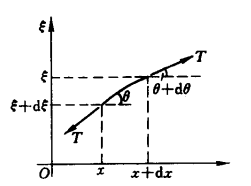
\includegraphics[height=90pt]{../assets/Vibration_of_String.png}
    \captionof{figure}{Demo of a string}
\end{center}

Consider the part of string in the picture Fig 4.1.

From Newton's Second Law of Motion (牛顿第二定律), we know that \[(\lambda \mathrm dx) {\partial^2 \xi \over \partial t^2 } = T \sin(\theta + \mathrm d\theta) - T \sin \theta.\]

Because \(\theta \ll 1\), we can approximate \(\sin \theta\) to \(\tan \theta\), and we can get: \begin{align*}
    (\lambda \mathrm dx) {\partial^2 \xi \over \partial t^2 } & = T \tan(\theta + \mathrm d\theta) - T \tan \theta \\
    & = T \left( \left. {\partial \xi \over \partial x} \right\vert _{x+\mathrm dx} - \left. {\partial \xi \over \partial x} \right \vert _x \right)\\
    & = T {\partial^2 \xi \over \partial x^2 } \mathrm dx,
\end{align*} and that brings us to \[\lambda {\partial^2 \xi \over \partial t^2 } = T {\partial^2 \xi \over \partial x^2 },\] \[{\lambda \over T} {\partial^2 \xi \over \partial t^2 } - {\partial^2 \xi \over \partial x^2 } = 0.\]

The velocity of the wave is \[c = \sqrt{T \over \lambda},\] and we can get \[{1 \over c^2} {\partial^2 \xi \over \partial t^2 } - {\partial^2 \xi \over \partial x^2 } = 0.\]

The equation above is on one dimension \(x\) only, and we can expand it to multiple dimensions \[{1 \over c^2} {\partial^2 \xi \over \partial t^2 } - \nabla ^2 \xi = 0,\] which is \[\left ( {1 \over c^2} {\partial^2 \over \partial t^2 } - \nabla ^2 \right ) \xi = \Box \xi = 0.\]

\section{Zero-Point Energy 零点能}\label{zero-point-energy-ux96f6ux70b9ux80fd}

\subsection*{(1) Simple Harmonic Oscillator 简谐振子}\label{simple-harmonic-oscillator-ux7b80ux8c10ux632fux5b50-1}

In classical mechanics we can have an SHO system, whose function can be written in the following ways:

\paragraph{Newtonian Mechanics 牛顿力学}\label{newtonian-mechanics-ux725bux987fux529bux5b66}

\[m \ddot x = -kx\] \[\ddot x + {k \over m } x =0 \] \[\ddot x + \omega^2 x =0, \ \omega=\sqrt{k \over m }.\]

\paragraph{Theoretical Mechanics 理论力学}\label{theoretical-mechanics-ux7406ux8bbaux529bux5b66}

\[L=T-V = {1 \over 2}m \dot x^2-{1 \over 2}k x^2\] \[{\partial L \over \partial \dot x} = m \dot x\] \[{\partial L \over \partial x} = -kx\]

From \[{\mathrm d \over \mathrm dt} {\partial L \over \partial \dot x}- {\partial L \over \partial x}=0,\] we know that \[{\mathrm d(m \dot x) \over \mathrm dt} - (-kx)=0, \] which is \[m \ddot x +kx = 0.\] \[\ddot x + \omega^2 x =0, \ \omega=\sqrt{k \over m }.\]

\subsection*{(2) Calculation of the zero-point energy 计算零点能}\label{calculation-of-the-zero-point-energy-ux8ba1ux7b97ux96f6ux70b9ux80fd}

Zero-point energy (ZPE) is the lowest possible energy that a quantum mechanical system may have.

Put the SHO system under quantum state (it becomes a \textbf{quantum harmonic oscillator} 量子谐振子), and we can get a minimum energy for it.

To calculate this ``minimum energy'', we start from Heisenberg Uncertainty Principle: \[\Delta x \cdot \Delta p \geq {\hbar \over 2}.\]

For the \textbf{lowest possible} energy, we need to have \[\Delta x \cdot \Delta p = {\hbar \over 2},\] which means \[\Delta p = {\hbar \over 2 \Delta x }.\]

From energy \[E = \dfrac{p^2}{2m}+ U = \dfrac{p^2}{2m} + {1 \over 2} m \omega^2 x^2,\] we can see that \begin{align*}
    \Delta E & = \dfrac{(\Delta p)^2}{2m} + {1 \over 2} m \omega^2 (\Delta x)^2 \\
    & = {{\left(\dfrac{\hbar}{ 2 \Delta x }\right)}^2 \over 2m} + {1 \over 2} m \omega^2 (\Delta x)^2 \\
    & = {\hbar^2 \over 8m(\Delta x)^2} + {1 \over 2} m \omega^2 (\Delta x)^2 \\
    & \geq 2 \sqrt{{\hbar^2 \over 8m(\Delta x)^2} \cdot {1 \over 2} m \omega^2 (\Delta x)^2} \\
    & = {\hbar \omega \over 2},
\end{align*} where \(=\) holds \textbf{if and only if} \[{\hbar^2 \over 8m(\Delta x)^2} = {1 \over 2} m \omega^2 (\Delta x)^2,\] that is, \[\Delta x = \sqrt{\hbar \over 2 m \omega}.\]

\emph{有些学着很聪明,以为什么都懂,但是其实他只懂了30\%。}
\emph{有些学者看起来呆头呆脑,但是呆头呆脑的人做研究做得踏实,这才是我们真正需要的大聪明。}

\section{Stationary Schrödinger Equation 定态薛定谔方程}\label{stationary-schruxf6dinger-equation-ux5b9aux6001ux859bux5b9aux8c14ux65b9ux7a0b}

We have the wave function \(\Psi(x, t)\).

We can perform \textbf{separation of variables (分离变量)} to the function and have \[\Psi(x, t) = \Phi(x) \cdot \mathcal{T}(t).\]

From \[-{ \hbar^2 \over 2m }{\partial^2 \Psi(x, t) \over \partial x ^2 } + U \Psi(x, t) =\mathrm i\hbar {\partial \Psi(x, t) \over \partial t},\] we can get \[-{ \hbar^2 \over 2m } \mathcal{T}(t){\mathrm d^2 \Phi(x) \over \mathrm d x ^2 } + U \Phi(x) \mathcal{T}(t) =\mathrm i\hbar \Phi(x) {\mathrm d \mathcal{T}(t) \over \mathrm d t}.\]

Put \(\Phi\) and \(x\) on one side and \(\mathcal{T}\) and \(t\) on the other, and we can get \[\dfrac{-\dfrac{ \hbar^2 }{2m}\dfrac{\mathrm d^2 \Phi(x)}{\mathrm d x ^2 } + U \Phi(x) }{\Phi(x)} = \dfrac{\mathrm i\hbar \dfrac{\mathrm d \mathcal{T}(t) }{\mathrm d t}}{\mathcal{T}(t)}.\]

Because \textbf{all \(\Phi\) and \(x\) are on the left side and all \(\mathcal{T}\) and \(t\) are on the right}, this equation can only hold \textbf{if this equation is equal to a constant}, that is, \[\dfrac{-\dfrac{ \hbar^2 }{2m}\dfrac{\mathrm d^2 \Phi(x)}{\mathrm d x ^2 } + U \Phi(x) }{\Phi(x)} = \dfrac{\mathrm i\hbar \dfrac{\mathrm d \mathcal{T}(t) }{\mathrm d t}}{\mathcal{T}(t)}=\mathrm{const}.\]

Perform dimensional analysis (量纲分析) on the equation above and we can see that the dimension of the constant is energy (\(\mathrm{M^1L^2T^{-2}}\)).

Let this constant be \(E\), and \(E\) is called the \textbf{eigenenergy} (能量的本征值).

Let's look at the two parts separately:

\subsection*{(1)\({\mathcal{T}(t)}\)}\label{mathcaltt}

The right part is equal to \(E\), which means that \begin{align*}
    \dfrac{\mathrm i\hbar \dfrac{\mathrm d \mathcal{T}(t) }{\mathrm d t}}{\mathcal{T}(t)} & =E \\
    \dfrac{\mathrm d \mathcal{T}(t) }{\mathcal{T}(t)} & = -{\mathrm iE \over \hbar}\mathrm dt \\
    \int {\dfrac{\mathrm d \mathcal{T}(t) }{\mathcal{T}(t)}} & = -{\mathrm iE \over \hbar} \int {\mathrm dt} \\
    \ln \mathcal{T}(t) & = -{\mathrm iE \over \hbar} t +C \\
    \mathrm e^{\ln \mathcal{T}(t)} & = \mathrm e^{- \mathrm iEt / \hbar +C} \\
    \mathcal{T}(t) & = \mathcal{T}_0 \cdot \mathrm e^{- \mathrm iEt / \hbar},
\end{align*} where \(C\) is the constant of integration (积分常数), and \(\mathrm e^C = \mathcal{T}_0\).

\subsection*{(2)\(\Phi(x)\)}\label{phix}

We can easily get this equation which does not include time \(t\) in it: \[-\dfrac{ \hbar^2 }{2m}\dfrac{\mathrm d^2 \Phi(x)}{\mathrm d x ^2 } + U \Phi(x) =E\Phi(x),\] which is called \textbf{Stationary Schrödinger Equation (定态薛定谔方程)}.

Under the SHO case, \(U=\dfrac{1}{2}m\omega^2x^2\), and we have \[-\dfrac{ \hbar^2 }{2m}\dfrac{\mathrm d^2 \Phi(x)}{\mathrm d x ^2 } + \dfrac{1}{2}m\omega^2x^2 \Phi(x) =E\Phi(x).\] Its general solution is \[\Phi^*(x) = C \exp(-{\alpha \over 2} x^2).\]

Find the first and second order derivatives for \(\Phi^*\):

\[{\mathrm d\Phi^*(x) \over \mathrm dx} = -\alpha x\cdot C \exp(-{\alpha \over 2} x^2) = -\alpha x \cdot \Phi^*(x)\]

\[{\mathrm d^2\Phi^*(x) \over \mathrm dx^2} = -\alpha (1-\alpha x^2) \cdot C \exp(-{\alpha \over 2} x^2) = -\alpha (1-\alpha x^2) \cdot \Phi^*(x)\]

And we have \[-\dfrac{ \hbar^2 }{2m}(-\alpha)(1-\alpha x^2)\cdot \Phi^*(x)+\dfrac{1}{2}m\omega^2x^2 \Phi^*(x)=E \Phi^*(x)\]

\[-\dfrac{ \hbar^2 }{2m}(-\alpha)(1-\alpha x^2)+\dfrac{1}{2}m\omega^2x^2 =E \]

\[\dfrac{\alpha \hbar^2 }{2m}(1-\alpha x^2) = E\left(1 - \dfrac{m\omega^2}{2E}x^2\right).\]

Compare the two forms and we know that \[\left \{
\begin {array}{l}
    \dfrac{\alpha \hbar^2 }{2m} = E, \\[1.5ex]
    \alpha = \dfrac{m\omega^2}{2E},
    \end {array}
    \right.\] and we get \[\left \{
    \begin {array}{l}
    E = \dfrac{\omega \hbar}{2}, \\[1.5ex]
    \alpha = \dfrac{m\omega}{\hbar}.
\end {array}
\right.\]

\chapter{2023/9/25}\label{20230925}

\section{Gravity and gravitational potential 引力和引力势}\label{gravity-and-gravitational-potential-ux5f15ux529bux548cux5f15ux529bux52bf}

The gravitational potential at \(r\) is \[U = - {GMm \over r},\] and the force there is \[\boldsymbol F(\boldsymbol r) = - \nabla U = - {GMm \over r^2} \hat {\boldsymbol r}.\]

\emph{为什么有\(r^2\)项?因为场是点源产生的球面场,场对应的力有\(r^2\)形式。}

We can integrate \(\boldsymbol F(\boldsymbol r)\) to get \(U(r_0)\): \[U(r_0) = \int^{+\infty}_{r_0} -{GMm \over r^2} \mathrm dr = \left.{GMm \over r} \right\vert^{+\infty}_{r_0} = -{GMm \over r_0}.\]

Near the ground of earth, at height \(h(h \ll R)\), we can have approximately \(U=mgh\). That's because \[U(R+h)- U(R)  = {GMm \over R} - {GMm \over R+h} = GMm \cdot {h \over R(R+h)} \approx {GMmh \over r^2} = mgh.\]

\section{The Great Debate for String, 1730\textasciitilde1780}\label{the-great-debate-for-string-17301780}

\begin{itemize}
\tightlist{}
\item
  Daniel Bernoulli: the first to propose a partial differential equation
  第一个提出偏微分方程的人
\item
  D'Alembert: superposition principle 叠加原理
\item
  Lagrange
\item
  Euler
\end{itemize}

John Bernoulli: the discretization of string vibration (弦振动的离散化), which sees the string as a string of beads (珠子).

\section{Gauss's theorem (electromagnetics) 高斯定理}\label{gausss-theorem-electromagnetics-ux9ad8ux65afux5b9aux7406}

\emph{The three most renowned mathematicians: Archimedes (阿基米德), Isaac Newton (伊萨克·牛顿), and \textbf{Gauss} (高斯).}

Differential form (微分形式): \[\nabla \cdot \boldsymbol E = {\rho \over \varepsilon_0}, \] or integral form (积分形式): \[\oiint_{\partial V} \boldsymbol E \cdot \mathrm d \boldsymbol S = {Q_{\mathrm{enc}} \over \varepsilon_0},\] in which ``\(\mathrm {enc}\)'' stands for \textbf{enclosed}.

\chapter{2023/9/27}\label{20230927}

\section{Quantum operators
量子算符}\label{quantum-operators-ux91cfux5b50ux7b97ux7b26}

\begin{itemize}
\tightlist{}
\item
  Momentum: \[\hat {\boldsymbol p} = - \mathrm i \hbar \nabla \]
\item
  Energy: \[\hat E = \mathrm i \hbar \dfrac{\partial}{\partial t} \]
\item
  Angular momentum: \begin{align*}
    \hat {\boldsymbol L} & = \boldsymbol r \times \hat {\boldsymbol p} \\ 
    & = (x \hat i + y \hat j + z \hat k) \times(- \mathrm i \hbar \nabla) \\
    & = \mathrm i \hbar\left[\left(z {\partial \over \partial y} - y {\partial \over \partial z} \right)\hat i + \left(x {\partial \over \partial z} - z {\partial \over \partial x} \right) \hat j + \left(y {\partial \over \partial x} - x {\partial \over \partial y} \right) \hat k \right]
    \end{align*}
\end{itemize}

\section{Vectors: flux and circulation
矢量:通量和环量}\label{vectors-flux-and-circulation-ux77e2ux91cfux901aux91cfux548cux73afux91cf}

\subsection*{(1) Definition 定义}\label{definition-ux5b9aux4e49}

\begin{itemize}
\tightlist{}
\item
  The flux (通量) of \(\boldsymbol A\) is defined as
  \[ \oiint_{\partial V} \boldsymbol A \cdot \mathrm d \boldsymbol S\]
  Gauss's divergence theorem (高斯散度定理):
  \[\iiint (\nabla \cdot \boldsymbol F) \mathrm dV = \oiint_{\partial V} \boldsymbol F \cdot \mathrm d \boldsymbol S\]
\item
  The circulation of \(\boldsymbol A\) is defined as
  \[\oint \boldsymbol A \cdot \mathrm d \boldsymbol l\] Stokes' theorem (斯托克斯公式):
  \[\oiint_{\partial V} (\nabla \times \boldsymbol A) \cdot \mathrm d \boldsymbol S = \oint \boldsymbol A \cdot \mathrm d \boldsymbol l.\]
\end{itemize}

\subsection*{(2) 3 equivalent conditions a conservative force field satisfies 保守立场满足的三个等价条件}\label{equivalent-conditions-a-conservative-force-field-satisfies-ux4fddux5b88ux7acbux573aux6ee1ux8db3ux7684ux4e09ux4e2aux7b49ux4ef7ux6761ux4ef6}

\begin{align*}
    \nabla \times \boldsymbol f = \boldsymbol 0 \quad(1) \\
    \oint \boldsymbol f \cdot \mathrm d \boldsymbol r = 0 \quad(2) \\
    \boldsymbol f = - \nabla \varphi \quad(3)
\end{align*}

Proof of equivalency 证明等价性:

\paragraph{\((1) \Rightarrow (2)\):}\label{rightarrow-2}

\[\oint \boldsymbol f \cdot \mathrm d \boldsymbol r = \oiint_{\partial V} (\nabla \times \boldsymbol f) \cdot \mathrm d \boldsymbol S = 0\]

\paragraph{\((2) \Rightarrow (3)\):}\label{rightarrow-3}

\[\mathrm dW = \boldsymbol f \cdot \mathrm d \boldsymbol r + \mathrm dU = 0\] \[\boldsymbol f \cdot \mathrm d \boldsymbol r = - \mathrm dU(\boldsymbol r) \] \[\boldsymbol f \cdot \mathrm d \boldsymbol r = - {\mathrm dU \over \mathrm d \boldsymbol r } \cdot \mathrm d \boldsymbol r \] \[\boldsymbol f = - {\mathrm dU \over \mathrm d \boldsymbol r } = - \nabla U \]

\paragraph{\((3) \Rightarrow (1)\): It's obvious. We skipped it.}\label{rightarrow-1-its-obvious.-we-skipped-it.}

\subsection*{(3) Examples:}\label{examples}

\paragraph{(1) In electromagnetics}\label{in-electromagnetics}

\[\boldsymbol J = \rho \boldsymbol v_d\] \[{\partial \rho \over \partial t} + \nabla \cdot \boldsymbol J = {\partial \rho \over \partial t}+\nabla \cdot (\rho \boldsymbol v_d) = 0\] In this, \(\nabla \cdot \boldsymbol J\) is a flux.

\paragraph{(2) Diffusion}\label{diffusion}

\[{\partial c \over \partial t} + \nabla \cdot \boldsymbol J = 0\] \[\boldsymbol J = - D \nabla c \text{\ \ (Fick's\  first\ law\ 菲克第一定律)}\] \[{\partial c \over \partial t} = - \nabla \cdot \boldsymbol J = D \nabla^2 c.\]

\section{Dimension homogeneity principle 量纲一致性原理}\label{dimension-homogeneity-principle-ux91cfux7eb2ux4e00ux81f4ux6027ux539fux7406}

In mechanics, there are only three dimensions involved: \(\mathrm{M}\) (mass), \(\mathrm{L}\) (length), and \(\mathrm{T}\) (time).

Dimension homogeneity principle includes three aspects: \begin{itemize}
\tightlist{}
\item Fundamental dimension 物理量
\item Rank 阶
\item Covariant and contravariant 协变和逆变
\end{itemize}

For example:

\emph{下面的大家自己推导量纲分析,5秒钟推不出来就是脑子有问题 (bushi)}

\begin{itemize}
\tightlist{}
\item
  Bernoulli's principle 伯努利原理
  \[p + {1 \over 2} \rho v^2 + \rho gh = \mathrm{const}\]
\item
  Navier-Stokes equations 纳维-斯托克斯方程
  \[ {\partial \boldsymbol v \over \partial t} +(\boldsymbol v \cdot \nabla) \boldsymbol v = - {1 \over \rho} \nabla p + \mu \nabla^2 \boldsymbol v + \boldsymbol g\]
\item
  Fourier's law of thermal conduction 傅里叶热传导定律
  \[\boldsymbol J = -k \nabla T\] \[\rho c {\partial T \over \partial t} + \nabla \cdot \boldsymbol J=0 \ \  (*)\]
\end{itemize}

\begin{quote}
作业:推导\((*)\)方程.
\end{quote}

\begin{quote}
作业:将欧姆定律写成通量形式.
\end{quote}

\begin{itemize}
\tightlist{}
\item
  Gravitational wave 引力波: \[\Box h_{\mu\nu} = \mathbf{0}.\]
\end{itemize}

\emph{In 1905, Poincaré deducted that the velocity of the gravitational wave is the speed of light.}

\begin{itemize}
\tightlist{}
\item
  Einstein field equations 爱因斯坦引力场方程
  \[R_{\mu\nu}+ {1 \over 2} g_{\mu\nu}R = {8 \pi G \over c^4} T_{\mu\nu}.\]
\item
  Riemann metric tensor 黎曼度规张量
  \[g_{\mu\nu} = \eta_{\mu\nu} + h_{\mu\nu},\] where \(g_{\mu\nu}\)
  stands for the curve part, \(\eta_{\mu\nu}\) for the flat part, and
  \(g_{\mu\nu}\) for the fluctuation (挠动) part.
\end{itemize}

\section{Black holes}\label{black-holes}

Black holes have three conservatives: mass, charge and angular momentum.

% \begin{longtable}[]{@{}ll@{}}
% \toprule\noalign{}
% Black holes & Dump holes (哑洞) \\
% \midrule\noalign{}
% \endhead
% \bottomrule\noalign{}
% \endlastfoot
% event horizon (事件视界) & acoustic horizon (声学界限) \\
% \end{longtable}

\begin{center}
    \begin{tabular}{|c|c|}
        \hline
        \textbf{Black holes} & \textbf{Dump holes (哑洞)} \\
        \hline
        event horizon (事件视界) & acoustic horizon (声学界限) \\
        \hline
    \end{tabular}
    \captionof{table}{Comparison of Black Holes and Dump Holes}
\end{center}

\begin{quote}
作业:哑洞是什么?
\end{quote}

Using dialectics (辩证法), we can know that things called ``white
holes'' should exist, and black and white holes are connected by
wormholes. There may exist parallel universes.

\begin{quote}
作业:什么是平行宇宙?
\end{quote}

\chapter{2023/10/9}\label{20231009}

\section{2023 Nobel Prize}\label{nobel-prize}

\subsection*{(1) The Nobel Prize in Physics
2023}\label{the-nobel-prize-in-physics-2023}

The Royal Swedish Academy of Sciences has decided to award the Nobel
Prize in Physics 2023 to:

\begin{itemize}
\tightlist{}
\item
  \textbf{Pierre Agostini} (The Ohio State University, Columbus, USA)
\item
  \textbf{Ferenc Krausz} (Max Planck Institute of Quantum Optics,
  Garching and Ludwig-Maximilians-Universität München, Germany)
\item
  \textbf{Anne L'Huillier} (Lund University, Sweden)
\end{itemize}

for \textbf{experimental methods that generate attosecond pulses of
light for the study of electron dynamics in matter}
(产生阿秒光脉冲用于研究物质中电子动力学的实验方法).
\[1 \ \mathrm{attosecond \ (as)} = 10^{-18} \mathrm{s}.\]

We can look at the scale of a hydrogen atom:
\[r \approx 5.3 \times 10^{-10} \ \mathrm{m},\]
\[v \approx 2.2 \times 10^{-6} \ \mathrm{m/s},\]
\[T = {2 \pi r \over v} = 1.52 \times 10^{-16} \ \mathrm{s} = 152 \ \mathrm{as}.\]

Another prize related: The Nobel Prize in Chemistry 1999 was awarded to
Ahmed H. Zewail ``for his studies of the transition states of chemical
reactions using femtosecond spectroscopy''
(利用飞秒光谱法对化学反应过渡态的研究).
\[1 \ \mathrm{femtosecond \ (fs)} = 10^{-15} \mathrm{s}.\]

\subsection*{(2) The Nobel Prize in Chemistry
2023}\label{the-nobel-prize-in-chemistry-2023}

The Royal Swedish Academy of Sciences has decided to award the Nobel
Prize in Chemistry 2023 to

\begin{itemize}
\tightlist{}
\item
  \textbf{Moungi G. Bawendi} Massachusetts Institute of Technology
  (MIT), Cambridge, MA, USA
\item
  \textbf{Louis E. Brus} Columbia University, New York, NY, USA
\item
  \textbf{Alexei I. Ekimov} Nanocrystals Technology Inc., New York, NY,
  USA
\end{itemize}

for \textbf{the discovery and synthesis of quantum dots}.

Confinement (限域效应)

\subsection*{(3) The Nobel Prize in Physiology or Medicine
2023}\label{the-nobel-prize-in-physiology-or-medicine-2023}

The Nobel Assembly at Karolinska Institutet has today decided to award
the 2023 Nobel Prize in Physiology or Medicine jointly to

\begin{itemize}
\tightlist{}
\item
  \textbf{Katalin Karikó}
\item
  \textbf{Drew Weissman}
\end{itemize}

for \textbf{their discoveries concerning nucleoside base modifications
that enabled the development of effective mRNA vaccines against
COVID-19}.

\section{Nondimensionalization
无量纲化}\label{nondimensionalization-ux65e0ux91cfux7eb2ux5316}

Advantages:
\begin{itemize}
\tightlist{}
\item Not restricted by unit systems
\item Guaranteed by similarity
\item Able to be applied widely
\end{itemize}

Take the nondimensionalization of the Navier-Stokes equations
纳维-斯托克斯方程:
\[ \underbrace{\partial \boldsymbol v \over \partial t}_{\text{Euler acceleration}} +\underbrace{(\boldsymbol v \cdot \nabla) \boldsymbol v}_{\text{Advective acceleration (non-linear)}} = -{1 \over \rho} \nabla p + \nu \nabla^2 \boldsymbol v\]

\begin{enumerate}
\def\labelenumi{\arabic{enumi}.}
\item
  Choose characteristic values:

  \begin{itemize}
\tightlist{}
  \item
    characteristic velocity 特征速度 \(V_0\)
  \item
    characteristic length 特征尺度 \(L_0\)
  \end{itemize}

  \begin{quote}
  作业:什么叫数量级 (order of magnitude)
  \end{quote}

  We can then use the values above to express the following:

  \begin{itemize}
\tightlist{}
  \item
    characteristic time 特征时间 \(T_0 = \dfrac{L_0}{V_0}\)
  \item
    characteristic pressure 特征压强 (temporarily unknown)
  \end{itemize}
\item
  Mark \textbf{dimensionless (or non-dimensional) values} with an
  asterisk (*) (无量纲的量用*作区分).
\item
  Replace the physical quantities in the original equation with
  dimensionless values.
\end{enumerate}

In this case, \(\boldsymbol v\) shall be replaced by
\(V_0 \cdot \boldsymbol v^*\), \(t\) by \(\dfrac{L_0}{V_0} t^*\),
\(\nabla\) by \(\dfrac{1}{L_0} \nabla^*\).

So the original equation \[{\partial \boldsymbol v \over \partial t} + (\boldsymbol v \cdot \nabla) \boldsymbol v = - {1 \over \rho} \nabla p + \nu \nabla^2 \boldsymbol v\] becomes:
\[ {\partial (V_0 \cdot \boldsymbol v^*) \over \partial \left(\dfrac{L_0}{V_0} t^*\right)} + \left[ (V_0 \cdot \boldsymbol v^*) \cdot \left( \dfrac{1}{L_0} \nabla^* \right) \right] (V_0 \cdot \boldsymbol v^*) = -{1 \over \rho} \left( \dfrac{1}{L_0} \nabla^* \right) p + \nu \cdot \left( \dfrac{1}{L_0} \nabla^* \right)^2 (V_0 \cdot \boldsymbol v^*)\]
\[{V_0^2 \over L_0} \left[{\partial \boldsymbol v^* \over \partial t^*} + (\boldsymbol v^* \cdot \nabla^*) \boldsymbol v^*\right] = - {1 \over \rho L_0}\nabla^* p + {\nu V_0 \over L_0^2} \nabla^{*2} \boldsymbol v^*\]
\[{\partial \boldsymbol v^* \over \partial t^*} + (\boldsymbol v^* \cdot \nabla^*) \boldsymbol v^* = - {1 \over \rho V_0^2}\nabla^* p + {\nu \over V_0 L_0} \nabla^{*2} \boldsymbol v^*.\]

Let \(\displaystyle p^* = {p \over \rho v_0^2}\), which fills the
\textbf{characteristic pressure} gap mentioned above, and Reynolds
number (雷诺数)
\[Re = {V_0L_0 \over \nu} = {\rho V_0L_0 \over \mu} \ (\nu = {\mu \over \rho}),\]
and the equation becomes
\[{\partial \boldsymbol v^* \over \partial t^*} + (\boldsymbol v^* \cdot \nabla^*) \boldsymbol v^* = - \nabla^* p^* + {1 \over Re} \nabla^{*2} \boldsymbol v^*.\]

\begin{quote}
作业:非线性项雷诺数的推导 (?)
\end{quote}

\section{Mass 质量}\label{mass-ux8d28ux91cf}

There are two types of masses:

\begin{itemize}
\tightlist{}
\item
  Inertia mass 惯性质量 \(m_i\) \[\boldsymbol F = m_i \boldsymbol a\]
\item
  Gravitational mass 引力质量 \(m_g\)
  \[\boldsymbol F = {GMm_g \over r^2} \hat{\boldsymbol r} \]
\end{itemize}

According to the equivalence principle (等效原理), it holds that
\[m_i \equiv m_g.\]

\begin{quote}
作业:什么是爱因斯坦的电梯思想实验?局域性指什么?
\end{quote}

There are two forms of the equivalence principle: the \textbf{weak}
equivalence principle (WEP for short) and the \textbf{strong}
equivalence principle.

We know that positive matter meets with WEP. But, does antimatter?

(27 September 2023 on 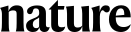
\includegraphics[height=10pt]{assets/Nature.png}: \emph{Observation of the effect of gravity on the motion of antimatter} (\url{https://doi.org/10.1038/s41586-023-06527-1}) and \emph{Free-falling antihydrogen reveals the effect of gravity on antimatter} (\url{https://doi.org/10.1038/d41586-023-02930-w}).)

\chapter{2023/10/11}\label{20231011}

\section{Phase an group velocity
相速度和群速度}\label{phase-an-group-velocity-ux76f8ux901fux5ea6ux548cux7fa4ux901fux5ea6}

Phase velocity (相速度) \(v_p\) is the velocity of a certain phase that
travels: \[v_p = {\omega \over k}.\]

Group velocity (群速度) \(v_g\) is the velocity with which the envelope
of the wave (波包) propagates through space:
\[v_g = {\Delta \omega \over \Delta k}.\]

Energy is transmitted through \emph{group velocity}, not \emph{phase
velocity}.

\begin{quote}
For more reference, you can see:
\url{https://www.zhihu.com/question/29444240/answer/1833520606}.
\end{quote}

\section{Order of magnitude
数量级}\label{order-of-magnitude-ux6570ux91cfux7ea7}

For a number \(N\), we usually define its order of magnitude as follows:

Write the number in the form \[N =a \times 10 ^ b,\] in which
\[\dfrac{1}{\sqrt{10}} \leq a \leq \sqrt{10}, b \in \mathbb{Q},\] and
\(b\) is the \textbf{order of magnitude} of the number. For example:

\begin{center}
    \begin{tabular}{|c|c|c|}
        \hline
        $N$ & Expression in $N =a \times 10^b$ & Order of magnitude $b$ \\
        \hline
        $0.2$ & $2 \times 10^{-1}$ & $-1$ \\
        $1$ & $1 \times 10^{0}$ & $0$ \\
        $5$ & $0.5 \times 10^{1}$ & $1$ \\
        $6$ & $0.6 \times 10^{1}$ & $1$ \\
        $31$ & $3.1 \times 10^{1}$ & $1$ \\
        $32$ & $0.32 \times 10^{2}$ & $2$ \\
        $999$ & $0.999 \times 10^{3}$ & $3$ \\
        $1000$ & $1 \times 10^{3}$ & $3$ \\
        \hline
    \end{tabular}
    \captionof{table}{Order of Magnitude Examples}
\end{center}

Some constants in physics:

\begin{itemize}
\tightlist{}
\item
  Avogadro constant \(N_A = 6.02 \times 10^{23} \ \mathrm{mol^{-1}}\)
\item
  Reduced Planck constant
  \(\hbar = 1.054 \times 10^{-34} \ \mathrm{J \cdot s}\)
\item
  Speed of light \(c = 2.99792 \times 10^{8} \ \mathrm{m/s}\)
\item
  Boltzmann constant
  \(k_\mathrm{B} = 1.38 \times 10^{-23} \ \mathrm{J/K}\)
\item
  Fundamental charge \(e = 1.602 \times 10^{-19} \ \mathrm{C}\)
\item
  Universal gravitational constant
  \(G = 6.672 \times 10^{-11} \ \mathrm{N \cdot m^2/kg^2}\)
\end{itemize}

Note: This definition is not absolute. For example, some people tend to
use \(0.5 \leq a \leq 5\) or other criteria.

\section{A particular model
某个模型}\label{a-particular-model-ux67d0ux4e2aux6a21ux578b}

Below (Fig 8.1) is a container with two sides connected to each other by a small
hole.

To get the two sides to balance, we need to have \[\left\{
    \begin{aligned}
        & p_1 = p_2; \quad  &\text{pressure} &\\
        & T_1 = T_2; &\text{temperature} &\\
        & \mu_1 = \mu_2. &\text{chemical potential (化学势)} &
    \end{aligned}
\right.\]

\begin{center}
    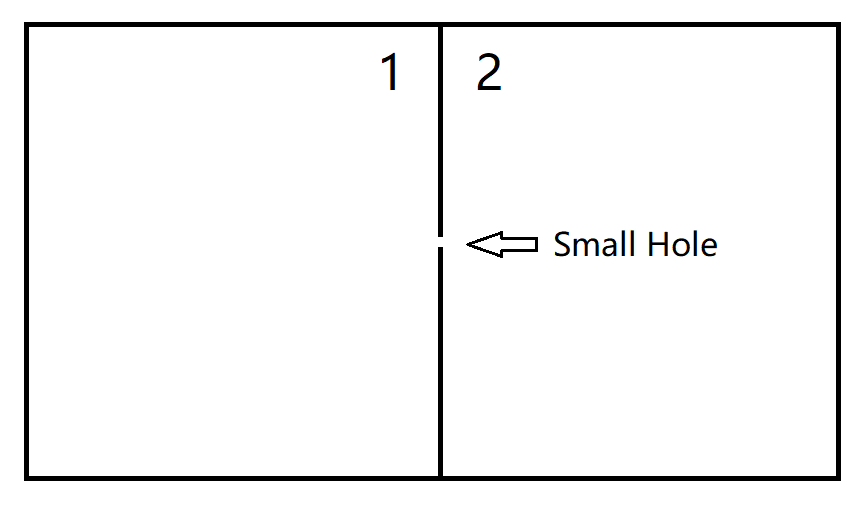
\includegraphics[height=100pt]{assets/Model_Two_sides.png}
    \captionof{figure}{A container with two sides}
\end{center}

Chemical potential \(\mu\) is defined as follows:

In a chemical system where there are \(n\) kinds of species (物种),
define \textbf{Gibbs free energy} (自由焓/吉布斯自由能) \[G=U-TS+pV\]
and the \textbf{chemical potential} (化学势) of species \(i\)
\[\mu_i = \left({\partial G \over \partial n_i}\right)_{T, p, n_j (j \neq i)}.\]

\section{About dimensional analysis and unit systems
关于量纲分析和单位制}\label{something-about-dimensional-analysis-and-unit-systems-ux4e00ux4e9bux5173ux4e8eux91cfux7eb2ux5206ux6790ux548cux5355ux4f4dux5236ux7684ux4e1cux897f}

Maxwell points out that:

\begin{enumerate}
\def\labelenumi{\arabic{enumi}.}
\item
  For a mechanical quantity (力学量), we only need three dimensions
  \(\mathrm{M, L, T}\) to form its unit and
\item
  Sometimes the dimensions of combined quantities (组合量的量纲) are
  more useful.
\end{enumerate}

There are two commonly-used unit systems in the world:

\begin{itemize}
\tightlist{}
\item \emph{Système
International} (SI) 国际单位制
\item Centimetre--gram--second system of units (CGS) 厘米--克--秒制
\end{itemize}

Let's look at a few examples.

\subsection*{(1) Coulomb's law
库仑定律}\label{coulombs-law-ux5e93ux4ed1ux5b9aux5f8b}

\[F = \left\{
\begin{aligned}
& \dfrac{q_1q_2}{4 \pi \varepsilon_0 r^2} & \text{(SI)} \\
& \dfrac{q_1q_2}{r^2} & \text{(CGS)}
\end {aligned}
\right.
\]

\subsection*{(2) Fine structure constant
精细结构常数}\label{fine-structure-constant-ux7cbeux7ec6ux7ed3ux6784ux5e38ux6570}

\[\alpha = \left\{
\begin{aligned}
& \dfrac{e^2}{4 \pi \varepsilon_0 \hbar c} & \text{(SI)} \\
& \dfrac{e^2}{\hbar c} & \text{(CGS)}
\end {aligned}
\right.
\approx {1 \over 137}.
\]

\emph{W. Pauli died in Room No.~137 in hospital. (地狱笑话了属于是)}

\subsection*{(3) Bohr radius
玻尔半径}\label{bohr-radius-ux73bbux5c14ux534aux5f84}

\[r_B = \left\{
\begin{aligned}
& \dfrac{4 \pi \varepsilon_0 \hbar^2}{m_e e^2} & \text{(SI)} \\
& \dfrac{\hbar^2}{m_ee^2} & \text{(CGS)}
\end {aligned}
\right.\]

\section{Planck units
普朗克单位}\label{planck-units-ux666eux6717ux514bux5355ux4f4d}

Planck units are a set of units that, by definition, are expressed using
these universal constants below, which, take the numeric value \(1\)
when expressed:

\begin{itemize}
\tightlist{}
\item
  the speed of light in vacuum \(c\)
\item
  the gravitational constant \(G\)
\item
  the reduced Planck constant \(\hbar\)
\item
  the Boltzmann constant \(k_\mathrm{B}\)
\end{itemize}

Typically we would use dimensional analysis to derive these units:
\[[c] = \mathrm{LT^{-1}};\]
\[[G] = {[F][r^2] \over [m_1m_2]} = \mathrm{\dfrac{ML}{T^2} \cdot L^2 \over M^2} = \mathrm{M^{-1}L^3T^{-2}};\]
\[[\hbar] = [E][t] = [mc^2][t] = \mathrm{ML^2T^{-1}};\]
\[[k_\mathrm{B}] = {[E] \over [T]} = {[mc^2] \over [T]} = \mathrm{ML^2T^{-2}\Theta^{-1}}.\]

\subsection*{(1) Planck length
普朗克长度}\label{planck-length-ux666eux6717ux514bux957fux5ea6}

\[\left[{G \hbar \over c^3}\right] = \mathrm{M^{-1}L^3T^{-2} \cdot ML^2T^{-1} \over (LT^{-1})^3} = \mathrm{L^2}.\]
\[l_P = \sqrt{G \hbar \over c^3}.\]

\subsection*{(2) Planck time
普朗克时间}\label{planck-time-ux666eux6717ux514bux65f6ux95f4}

\[t_P = {l_P \over c} = \sqrt{G \hbar \over c^5}.\]

\subsection*{(3) Planck mass
普朗克质量}\label{planck-mass-ux666eux6717ux514bux8d28ux91cf}

\[\left[{\hbar c \over G}\right]  = \mathrm{ML^2T^{-1} \cdot LT^{-1} \over M^{-1}L^3T^{-2}} = \mathrm{M^2}.\]
\[m_P = \sqrt{\hbar c\over G}.\]

\subsection*{(4) Planck temperature
普朗克温度}\label{planck-temperature-ux666eux6717ux514bux6e29ux5ea6}

\[\left[{\hbar c^5 \over Gk_\mathrm{B}^2}\right] = \mathrm{ML^2T^{-1} \cdot (LT^{-1})^5 \over M^{-1}L^3T^{-2} \cdot (ML^2T^{-2}\Theta^{-1})^2} = \mathrm{\Theta^2}.\]
\[T_P = \sqrt{\hbar c^5 \over Gk_\mathrm{B}^2}.\]

\subsection*{(5) Planck energy
普朗克能量}\label{planck-energy-ux666eux6717ux514bux80fdux91cf}

\[E_P = m_Pc^2 = \sqrt{\hbar c^5\over G}.\]

\subsection*{(6) Planck momentum
普朗克动量}\label{planck-momentum-ux666eux6717ux514bux52a8ux91cf}

\[p_P = m_Pc = \sqrt{\hbar c^3\over G}.\]

\subsection*{(7) Planck acceleration
普朗克加速度}\label{planck-acceleration-ux666eux6717ux514bux52a0ux901fux5ea6}

\[a_P = {c \over t_P} = \sqrt{c^7 \over \hbar G}.\]

\subsection*{(8) Planck force
普朗克力}\label{planck-force-ux666eux6717ux514bux529b}

\[F_P = m_P a_P = {c^4 \over G}.\]

Note that the Planck force can be \emph{hidden} in the Einstein
gravitational field equations: \[R_{\mu\nu} - {1 \over 2}g_{\mu\nu}R = 8 \pi \mathbf{G \over c^4}T_{\mu\nu} = {8 \pi \over \mathbf{F_P}} T_{\mu\nu}.\]

\emph{隐藏在引力方程中的力,被称为引力很合理吧?这恒河里!doge}

\subsection*{(9) Planck density
普朗克密度}\label{planck-density-ux666eux6717ux514bux5bc6ux5ea6}

\[\rho_P = {m_P \over {l_P}^3} = {c^5 \over \hbar G^2}.\]

\chapter{2023/10/16}\label{20231016}

\section{Something about dimension analysis and Planck units
一些关于量纲分析和普朗克单位的内容}\label{something-about-dimension-analysis-and-planck-units-ux4e00ux4e9bux5173ux4e8eux91cfux7eb2ux5206ux6790ux548cux666eux6717ux514bux5355ux4f4dux7684ux5185ux5bb9}

\subsection*{(1) Einstein radius
爱因斯坦角半径}\label{einstein-radius-ux7231ux56e0ux65afux5766ux89d2ux534aux5f84}

The Einstein radius, \(\theta_E\), is the radius of an Einstein ring,
and \[\theta_E = \sqrt{4GM \over c^2 \cdot D_r},\] where \(D_r\) is the
\emph{impact parameter} (the distance of nearest approach of the
lightbeam to the center of mass).

\subsection*{(2) Planck charge
普朗克电量}\label{planck-charge-ux666eux6717ux514bux7535ux91cf}

From the fine structure constant \(\alpha = \dfrac{e^2}{\hbar c}\)
(under \(\text{cgs}\) system), we can see that \[[e^2] = [\hbar c].\]
Therefore, we can define the Planck charge \[e_P = \sqrt{\hbar c}.\]

\section{Gauge transformation (by Hermann Weyl)
规范场变换}\label{gauge-transformation-by-hermann-weyl-ux89c4ux8303ux573aux53d8ux6362}

From the second equation of the Maxwell's equations \[\nabla \cdot \boldsymbol B = 0,\] we can see \(B\) as the curl of a certain vector \(\boldsymbol A\). We call this \(\boldsymbol A\)
\textbf{magnetic vector potential} (磁矢势), and
\[\boldsymbol B  = \nabla \times \boldsymbol A.\]

Because the curl of the gradient of a certain scalar (标量梯度的旋度) is zero, we can add the gradient of a scalar field \(\psi\): \[\boldsymbol A \mapsto \boldsymbol A + \nabla \psi, \quad  (*)\] and we get \[\boldsymbol B  = \nabla \times (\boldsymbol A + \nabla \psi).\]

Substitute \(\boldsymbol B\) in
\[\nabla \times \boldsymbol E = -{\partial \boldsymbol B \over \partial t},\]
and we can get
\[\nabla \times \boldsymbol E = - {\partial \over \partial t} \left( \nabla \times \boldsymbol A \right) = - \nabla \times {\partial \boldsymbol A \over \partial t}\]
\[\nabla \times \left(\boldsymbol E + {\partial \boldsymbol A \over \partial t} \right) = \boldsymbol 0.\]

From this, we can see
\(\boldsymbol E + \dfrac{\partial \boldsymbol A }{ \partial t}\) as the
negative of the gradient of a scalar field \(\varphi\) (标量场
\(\varphi\) 梯度的负), and
\[\boldsymbol E = - \dfrac{\partial \boldsymbol A }{ \partial t} - \nabla \varphi.\]

When we put in the \(\boldsymbol A\) shown by \((*)\), we can get:
\begin{align*}
    \boldsymbol E & = - \dfrac{\partial}{ \partial t}(\boldsymbol A + \nabla \psi) - \nabla \varphi \\
    & = - \dfrac{\partial \boldsymbol A }{ \partial t} - \nabla \left(\varphi + {\partial \psi \over \partial t}\right).
\end{align*}

This shows that, when we make the transformation below (\textbf{the gauge transformation} 规范变换) \[\left\{
    \begin{array} {l}
        \boldsymbol A \mapsto \boldsymbol A + \nabla \psi; \\
        \varphi \mapsto \varphi - \dfrac{\partial \psi}{\partial t}.
    \end{array}
\right.\]

We can ensure that the fields \(\boldsymbol B\) and \(\boldsymbol E\)
remain unchanged.

\section{The Kronecker Delta
克罗尼克符号}\label{the-kronecker-delta-ux514bux7f57ux5c3cux514bux7b26ux53f7}

We define the Kronecker Delta in this way: \[\delta_{ij} = \left\{
    \begin{aligned}
        1,\ \ &i = j \\
        0,\ \ &i \neq j
    \end{aligned}
\right.\]

Example of practical use:
\[\boldsymbol a \cdot \boldsymbol b = (a_i \boldsymbol e_i) \cdot (b_j \boldsymbol e_j) = a_ib_j \delta_{ij}.\]

\section{The Levi-Civita Symbol
列维-奇维塔符号}\label{the-levi-civita-symbol-ux5217ux7ef4-ux5947ux7ef4ux5854ux7b26ux53f7}

We define the Levi-Civita Symbol in this way:
\[\boldsymbol e_i \times \boldsymbol e_j = \varepsilon_{ijk} \boldsymbol e_k.\]
In other words, \[\varepsilon_{ijk} = \left\{
    \begin{aligned}
        1, & \ \ &\text{even permutation (偶置换)};  \\
        -1, & & \text{odd permutation (奇置换)};\\
        0, & & i=j \ \text{or} \ i = k \ \text{or} \ j = k \ \text{(有重合指标)}.
    \end{aligned}
\right.\]

In the following picture, the left is for even permutations, and the
right for odd permutations:

\begin{center}
    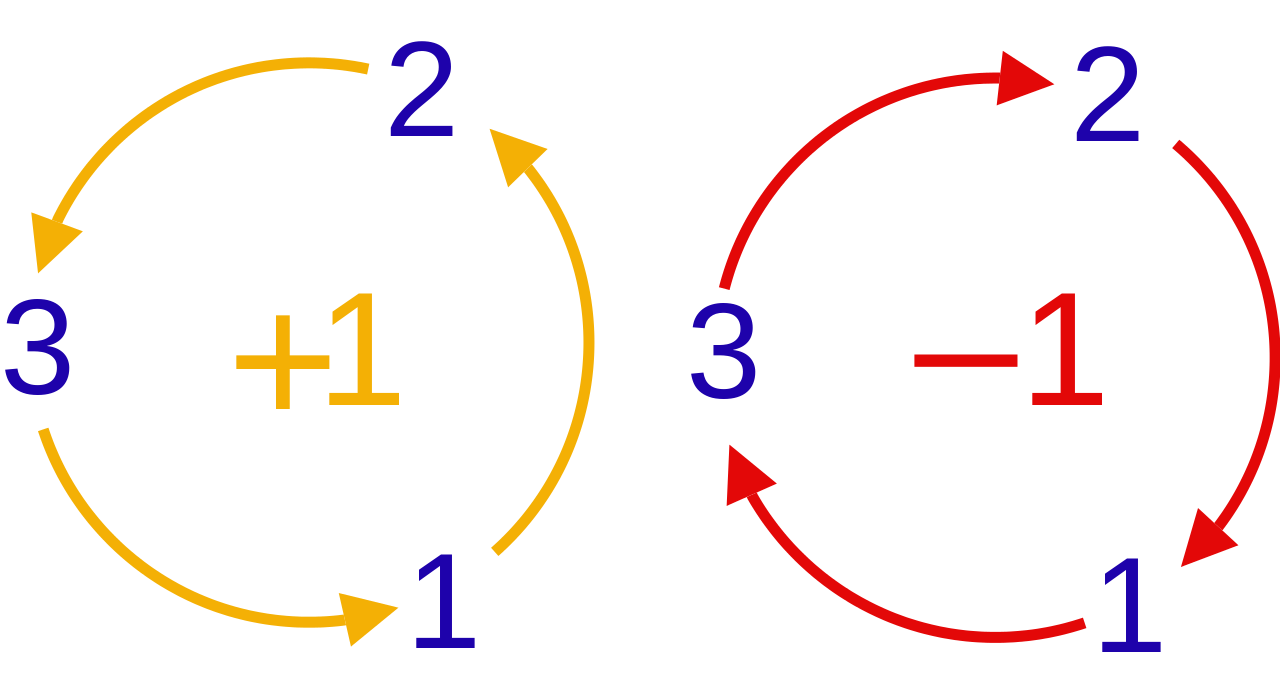
\includegraphics[height=80pt]{assets/Levi-Civita_Symbol.png}
    \captionof{figure}{Levi-Civita symbol (Source: Wikipedia)}
\end{center}

In word form, if \((i,j,k)\) is \((1,2,3)\), \((2,3,1)\) or \((3,1,2)\),
then \(\varepsilon_{ijk} = 1\). If \((i,j,k)\) is \((3,2,1)\),
\((1,3,2)\) or \((2,1,3)\), then \(\varepsilon_{ijk} = -1\).

Example of practical use:
\[\boldsymbol a \times \boldsymbol b = (a_i \boldsymbol e_i) \times (b_j \boldsymbol e_j) = a_ib_j \varepsilon_{ijk} \boldsymbol e_k.\]

\section{Einstein summation convention
爱因斯坦求和约定}\label{einstein-summation-convention-ux7231ux56e0ux65afux5766ux6c42ux548cux7ea6ux5b9a}

In this notation (标记法), when an index variable appears twice in a
single term and is not otherwise defined, it implies summation of that
term over all the values of the index.

For example, if index \(i\) ranges over the set \(\{1, 2, 3\}\), then \(y = c_ix^i\) means \[y = \sum_{i=1}^3 c_ix_i = c_1x_1 + c_2x_2 + c_3x_3.\]

An index that is summed over is a \textbf{summation index}, in this case
\(i\). It is also called a \textbf{dummy index (哑标)} since any symbol can
replace \(i\) without changing the meaning of the expression (provided
that it does not collide with other index symbols in the same term).

An index that is not summed over is a \textbf{free index} (自由指标) and
should appear only once per term. If such an index does appear, it
usually also appears in every other term in an equation. An example of a
free index is the \(i\) in the equation \(v_i = a_i b_j x^j\), which is
equivalent to the equation \(v_i = \sum_j(a_i b_j x^j)\).

Examples:

\subsection*{(1) Lorentz force}\label{lorentz-force}

\[\boldsymbol F = q(\boldsymbol E + \boldsymbol v \times \boldsymbol B)\]
\[F_k = q (E_k + v_i B_j \varepsilon_{ijk})\]

Dummy indices \(-\) \(i\), \(j\); Free index \(-\) \(k\)

\subsection*{(2) Maxwell's equations}\label{maxwells-equations}

\[\left\{
    \begin{aligned}
        &\dfrac{\partial E_i}{\partial x^i} = \dfrac{\rho}{\varepsilon_0} & \ \ &  i \text{ -- Dummy index}\\
        &\dfrac{\partial B_i}{\partial x^i} = 0 && i \text{ -- Dummy index}\\
        &\dfrac{\partial E_j}{\partial x_i}\varepsilon_{ijk} = - \dfrac{\partial B_k}{\partial t} && i, j \text{ -- Dummy indices;} \ k \text{ -- Free index}\\
        &\dfrac{\partial B_j}{\partial x_i}\varepsilon_{ijk} = \mu_0\left( j_k + \varepsilon_0\dfrac{\partial E_k}{\partial t}\right) && i, j \text{ -- Dummy indices;} \ k \text{ -- Free index}
    \end{aligned}
\right.\]

\chapter{2023/10/18}\label{20231018}

\section{Warming Up}\label{warming-up}

\subsection*{(1) In quantum mechanics:}\label{in-quantum-mechanics}

\[\hat {\boldsymbol L} = \boldsymbol r \times \hat {\boldsymbol p} = - \mathrm i \hbar \boldsymbol r \times \nabla = - \mathrm i \hbar (x_i \boldsymbol e_i) \times \left({\partial \over \partial x_j }\boldsymbol e_j\right)= - \mathrm i \hbar x_i {\partial \over \partial x_j } \varepsilon_{ijk} \boldsymbol e_k.\]

\subsection*{(2) Coriolis acceleration
科氏加速度}\label{coriolis-acceleration-ux79d1ux6c0fux52a0ux901fux5ea6}

\[a_\text{Cor} = 2 \boldsymbol \omega \times \boldsymbol v' = 2 \omega_i v_j' \varepsilon_{ijk} \boldsymbol e_k.\]

\section{Matrices and determinants
矩阵和行列式}\label{matrices-and-determinants-ux77e9ux9635ux548cux884cux5217ux5f0f}

\emph{(译者注:matrix的复数形式是matrices)}

Define matrix \(\mathbf A\): \[\mathbf A=
\begin{bmatrix}
    a_{11} & a_{12} & a_{13} \\
    a_{21} & a_{22} & a_{23} \\
    a_{31} & a_{32} & a_{33} \\
\end{bmatrix},\] where \(a_{rc}\) refers to the entry located in row
\(r\) and column \(c\).

For example, We can write the Kronecker delta in matrix form:
\[\delta_{ij} = \begin{bmatrix}
    1 & 0 & 0 & \ldots & 0 \\
    0 & 1 & 0 & \ldots & 0 \\
    0 & 0 & 1 & \ldots & 0 \\
    \vdots & \vdots & \vdots & \ddots & \vdots \\
    0 & 0 & 0 & \ldots & 1
\end{bmatrix} = \mathbf{I}.\]

And determinant (行列式) of \(\mathbf A\): \begin{align*}
    \det (\mathbf A) & =
    \begin{vmatrix}
        a_{11} & a_{12} & a_{13} \\
        a_{21} & a_{22} & a_{23} \\
        a_{31} & a_{32} & a_{33} \\
    \end{vmatrix} \\
    & = 
    a_{11} \begin{vmatrix}
        a_{22} & a_{23} \\
        a_{32} & a_{33} \\
    \end{vmatrix} + 
    a_{12} \begin{vmatrix}
        a_{23} & a_{21} \\
        a_{33} & a_{31} \\
    \end{vmatrix} + 
    a_{13} \begin{vmatrix}
        a_{21} & a_{22} \\
        a_{31} & a_{32} \\
    \end{vmatrix} \\
    & = a_{11}(a_{22}a_{33} - a_{23}a_{32}) + a_{12}(a_{23}a_{31} - a_{21}a_{33}) + a_{13}(a_{21}a_{32} - a_{22}a_{31} ) \\
    & = (a_{11}a_{22}a_{33} + a_{12}a_{23}a_{31} + a_{13}a_{21}a_{32}) - (a_{11}a_{23}a_{32} + a_{12}a_{21}a_{33} + a_{13}a_{22}a_{31}). \quad (*)
\end{align*}

In \((*)\), you can see that the first digit follows the even
permutation, and the second digit follows the even permutation (for
positive terms) and odd permutation (for negative terms).

We can put \(\det \mathbf A\) in \textbf{compact/component form}
(紧凑/指标形式):
\[\det(\mathbf{A}) = \varepsilon_{ijk} a_{1i} a_{2j} a_{3k} = \varepsilon_{\alpha \beta \gamma} a_{\alpha 1} a_{\beta 2} a_{\gamma 3}.\]

\section{The product of two Levi-Civita symbols
两个列维-奇维塔符号的乘积}\label{the-product-of-two-levi-civita-symbols-ux4e24ux4e2aux5217ux7ef4-ux5947ux7ef4ux5854ux7b26ux53f7ux7684ux4e58ux79ef}

The default situation, or one with no repeated indices is this:
\begin{align*}
    \varepsilon_{ijk}\varepsilon_{lmn} &= \begin{vmatrix}
        \delta_{i\ell} & \delta_{im} & \delta_{in} \\
        \delta_{j\ell} & \delta_{jm} & \delta_{jn} \\
        \delta_{k\ell} & \delta_{km} & \delta_{kn} \\
    \end{vmatrix} \\
    &= \delta_{i\ell}\left( \delta_{jm}\delta_{kn} - \delta_{jn}\delta_{km}\right) - \delta_{im}\left( \delta_{j\ell}\delta_{kn} - \delta_{jn}\delta_{k\ell} \right) + \delta_{in} \left( \delta_{j\ell}\delta_{km} - \delta_{jm}\delta_{k\ell} \right).
\end{align*}

Below, without special mentioning, we default to 3-dimensional
conditions.

\subsection*{(1) One repeated index
1个指标重复}\label{one-repeated-index-1ux4e2aux6307ux6807ux91cdux590d}

Let \(i=\ell\), and \begin{align*}
    \varepsilon_{ijk}\varepsilon^{imn} &= \begin{vmatrix}
        {\delta_i}^i & {\delta_i}^m & {\delta_i}^n \\
        {\delta_j}^i & {\delta_j}^m & {\delta_j}^n \\
        {\delta_k}^i & {\delta_k}^m & {\delta_k}^n \\
    \end{vmatrix} \\
    &= {\delta_i}^i \left( {\delta_j}^m {\delta_k}^n - {\delta_j}^n {\delta_k}^m \right) - {\delta_i}^m \left( {\delta_j}^i {\delta_k}^n - {\delta_j}^n {\delta_k}^i \right) + {\delta_i}^n \left( {\delta_j}^i {\delta_k}^m - {\delta_j}^m {\delta_k}^i \right) \\
    &= 3\left( {\delta_j}^m {\delta_k}^n - {\delta_j}^n {\delta_k}^m \right) - ({\delta_i}^m {\delta_j}^i) {\delta_k}^n + ({\delta_i}^m {\delta_k}^i) {\delta_j}^n + ({\delta_i}^n {\delta_j}^i) {\delta_k}^m - ({\delta_i}^n {\delta_k}^i) {\delta_j}^m \\
    &= 3\left( {\delta_j}^m {\delta_k}^n - {\delta_j}^n {\delta_k}^m \right) - {\delta_j}^m {\delta_k}^n + {\delta_k}^m {\delta_j}^n + {\delta_j}^n {\delta_k}^m - {\delta_k}^n {\delta_j}^m \\ 
    &= {\delta_j}^m {\delta_k}^n - {\delta_j}^n {\delta_k}^m.
\end{align*}

\emph{助记:正序 \(-\) 逆序}

Example: \begin{align*}
    \boldsymbol a \times \left(\boldsymbol b \times \boldsymbol c\right)
    & = \boldsymbol a \times \left(b_i\boldsymbol e_i \times c_j \boldsymbol e_j \right) \\
    & = \left(a_\ell \boldsymbol e_\ell \right) \times \left(b_i c_j \varepsilon_{ijk} \boldsymbol e_k \right) \\
    & = a_\ell b_i c_j \varepsilon_{ijk} \varepsilon_{\ell km} \boldsymbol e_m \\
    & = a_\ell b_i c_j \varepsilon_{ijk} \varepsilon_{m \ell k} \boldsymbol e_m \\
    & = a_\ell b_i c_j \left( \delta_{im}\delta_{j \ell} - \delta_{i \ell}\delta_{jm} \right) \boldsymbol e_m \\
    & = \underset{\text{Let } i = m,\ j = \ell}{\underline{a_j b_i c_j \boldsymbol e_i}} - \underset{\text{Let } i = \ell,\ j = m}{\underline{a_i b_i c_j \boldsymbol e_j}} \\
    & = \boldsymbol b  \left(\boldsymbol a \cdot \boldsymbol c \right) - \boldsymbol c \left(\boldsymbol a \cdot \boldsymbol b \right).
\end{align*}

\emph{助记:``back cab'' (后面的出租车)}

\subsection*{(2) Two repeated indices
2个指标重复}\label{two-repeated-indices-2ux4e2aux6307ux6807ux91cdux590d}

Let \(i=\ell, \ j = m\), and
\[\varepsilon_{ijk}\varepsilon^{ijn} = {\delta_j}^j {\delta_k}^n - {\delta_j}^n {\delta_k}^j = 3 {\delta_k}^n - {\delta_k}^n = 2 {\delta_k}^n.\]

\subsection*{(3) Three repeated indices
3个指标重复}\label{three-repeated-indices-3ux4e2aux6307ux6807ux91cdux590d}

Let \(i=\ell, \ j = m, \ k = n\), and
\[\varepsilon_{ijk}\varepsilon^{ijk} = 2 {\delta_k}^k = 6 = 3!.\]

Under \(n\) dimensions, where \(i_1, i_2, \cdots, i_n\) takes the values
\(1, 2, \cdots, n\), there is
\[\varepsilon_{i_1 i_2 \cdots i_n}\varepsilon^{i_1 i_2 \cdots i_n} = n!,\]
where the exclamation mark (\(!\)) denotes the factorial (阶乘).

\subsection*{(4) An example}\label{an-example}

A rigid body (刚体) is rotating at a constant angular velocity
\(\boldsymbol \omega_0\), and the velocity is
\[\boldsymbol v = \boldsymbol \omega_0 \times \boldsymbol r.\]

\begin{quote}
作业:用Levi-Civita符号展开上式。
\end{quote}

The curl of \(\boldsymbol v\) is \begin{align*}
    \nabla \times \left( \boldsymbol \omega_0 \times \boldsymbol r\right)
    & = {\partial \over \partial x_\ell} \boldsymbol e_\ell \times \left(\omega_{0, i} x_j \varepsilon_{ijk} \boldsymbol e_k \right) \\
    & = \omega_{0, i} {\partial x_j \over \partial x_\ell} \varepsilon_{ijk} \varepsilon_{lkm} \boldsymbol e_m \\
    & = \omega_{0, i} \delta_{j \ell} \varepsilon_{ijk} \varepsilon_{lkm} \boldsymbol e_m \\
    & = \omega_{0, i} \varepsilon_{ijk} \varepsilon_{jkm} \boldsymbol e_m \\
    & = \omega_{0, i} \varepsilon_{ijk} \varepsilon_{mjk} \boldsymbol e_m \\
    & = \omega_{0, i} \cdot 2 \delta_{im} \cdot \boldsymbol e_m \\
    & = 2 \omega_{0, i} \boldsymbol e_i \\
    & = 2 \boldsymbol \omega_0.
\end{align*}

\emph{This is ``Error in Beauty'' -- Sommerfeld}

\begin{quote}
作业:Feynman 的口诀:\begin{align*}
\nabla \times \left( \boldsymbol a \times \boldsymbol b \right) & = \nabla_{\boldsymbol a} \times \left( \boldsymbol a \times \boldsymbol b \right) + \nabla_{\boldsymbol b} \times \left( \boldsymbol a \times \boldsymbol b \right) \\
& = \boldsymbol a \left(\nabla_{\boldsymbol a} \cdot \boldsymbol b \right) - \boldsymbol b \left(\nabla_{\boldsymbol a} \cdot \boldsymbol a \right) + \boldsymbol a \left(\nabla_{\boldsymbol b} \cdot \boldsymbol b \right) - \boldsymbol b \left(\nabla_{\boldsymbol b} \cdot \boldsymbol a \right).
\end{align*}

表示上式。
\end{quote}

\chapter{2023/10/23}\label{20231023}

\begin{quote}
作业:黑洞熵是什么
\end{quote}

\emph{任正非:华为的自我批判性}

\section{Something about Levi-Civita symbols and matrices
关于列维-奇维塔符号和矩阵}\label{something-about-levi-civita-symbols-and-matrices-ux5173ux4e8eux5217ux7ef4-ux5947ux7ef4ux5854ux7b26ux53f7ux548cux77e9ux9635}

Consider a 3 by 3 matrix (\(3 \times 3\) 矩阵) \(\mathbf A\):
\[\mathbf A = \begin{bmatrix}
    a_{11} & a_{12} & a_{13} \\
    a_{21} & a_{22} & a_{23} \\
    a_{31} & a_{32} & a_{33} \\
\end{bmatrix}.\]

The determinant of \(\mathbf{A}\) is \begin{align*}
    \det (\mathbf A) & = \begin{vmatrix}
        a_{11} & a_{12} & a_{13} \\
        a_{21} & a_{22} & a_{23} \\
        a_{31} & a_{32} & a_{33} \\
    \end{vmatrix} \\
    & = \varepsilon_{\alpha \beta \gamma} a_{1 \alpha} a_{2 \beta} a_{3 \gamma} = \varepsilon_{\alpha \beta \gamma} a_{2 \alpha} a_{3 \beta} a_{1 \gamma} = \varepsilon_{\alpha \beta \gamma} a_{3 \alpha} a_{1 \beta} a_{2 \gamma} \\ 
    & = - \varepsilon_{\alpha \beta \gamma} a_{3 \alpha} a_{2 \beta} a_{1 \gamma} = - \varepsilon_{\alpha \beta \gamma} a_{1 \alpha} a_{3 \beta} a_{2 \gamma} = - \varepsilon_{\alpha \beta \gamma} a_{2 \alpha} a_{1 \beta} a_{3 \gamma}. \\ 
\end{align*}

Consider \((i, j, k)\) taking the following values, and \(\varepsilon_{ijk} \varepsilon_{\alpha \beta \gamma} a_{i \alpha} a_{j \beta} a_{k \gamma}\) will become respectively \begin{align*}
    \text{even} &
    \left\{
        \begin{aligned}
            (1, 2, 3) & \ \ \ & \varepsilon_{123} \varepsilon_{\alpha \beta \gamma} a_{1 \alpha} a_{2 \beta} a_{3 \gamma} & = \det (\mathbf A); \\
            (2, 3, 1) & \ \ \ & \varepsilon_{231} \varepsilon_{\alpha \beta \gamma} a_{2 \alpha} a_{3 \beta} a_{1 \gamma} & = \det (\mathbf A); \\
            (3, 1, 2) & \ \ \ & \varepsilon_{312} \varepsilon_{\alpha \beta \gamma} a_{3 \alpha} a_{1 \beta} a_{2 \gamma} & = \det (\mathbf A); \\
        \end{aligned}
    \right.
    \\
    \text{odd} &
    \left\{
        \begin{aligned}
            (3, 2, 1) & \ \ \ & \varepsilon_{321} \varepsilon_{\alpha \beta \gamma} a_{3 \alpha} a_{2 \beta} a_{1 \gamma} & = - \det (\mathbf A); \\
            (2, 1, 3) & \ \ \ & \varepsilon_{213} \varepsilon_{\alpha \beta \gamma} a_{2 \alpha} a_{1 \beta} a_{3 \gamma} & = - \det (\mathbf A); \\
            (1, 3, 2) & \ \ \ & \varepsilon_{132} \varepsilon_{\alpha \beta \gamma} a_{1 \alpha} a_{3 \beta} a_{2 \gamma} & = - \det (\mathbf A). \\
        \end{aligned}
    \right.
\end{align*}

Therefore, we can say
\[\det (\mathbf A) = {1 \over 6} \varepsilon_{ijk} \varepsilon_{\alpha \beta \gamma} a_{i \alpha} a_{j \beta} a_{k \gamma}.\]

\section{Deduction of electromagnetic wave equations
电磁波方程推导}\label{deduction-of-electromagnetic-wave-equations-ux7535ux78c1ux6ce2ux65b9ux7a0bux63a8ux5bfc}

In vacuum (真空), \(\rho = 0\) and
\(\boldsymbol j = \rho \boldsymbol v_d = \boldsymbol 0\), and Maxwell's
equations degenerate into the following form: \[\left \{
    \begin{array}{l} 
        \nabla \cdot \boldsymbol E = 0; \\
        \nabla \cdot \boldsymbol B = 0; \\
        \nabla \times \boldsymbol E = -\dfrac{\partial B}{\partial t}; \quad (*) \\[1.5ex]
        \nabla \times \boldsymbol B = \mu_0 \varepsilon_0 \dfrac{\partial \boldsymbol E}{ \partial t} = \dfrac{1}{c^2} \dfrac{\partial \boldsymbol E}{ \partial t}.
    \end{array} 
\right.\]

Get the curl of the left and right sides of \((*)\):

Left-hand side: \begin{align*}
    \nabla \times (\nabla \times \boldsymbol E) & = \nabla \times \left({\partial E_j \over \partial x_i} \varepsilon_{ijk} \boldsymbol e_k \right) \\
    & = \left({\partial \over \partial x_\ell} \boldsymbol e_\ell \right) \times \left({\partial E_j \over \partial x_i} \varepsilon_{ijk} \boldsymbol e_k \right) \\
    & = {\partial^2 E_j \over \partial x_i \partial x_\ell} \varepsilon_{ijk} \varepsilon_{\ell k m} \boldsymbol e_m \\
    & = {\partial^2 E_j \over \partial x_i \partial x_\ell} \varepsilon_{ijk} \varepsilon_{m \ell k} \boldsymbol e_m \\
\end{align*}
\begin{align*}
    & = {\partial^2 E_j \over \partial x_i \partial x_\ell} (\delta_{im}\delta_{j \ell} - \delta_{i \ell}\delta_{jm}) \boldsymbol e_m \\
    & = {\partial^2 E_j \over \partial x_i \partial x_j} \boldsymbol e_i - {\partial^2 E_j \over \partial x_i^2} \boldsymbol e_j \\
    & = \boldsymbol e_i {\partial \over \partial x_i}\left({\partial E_j \over \partial x_j}\right) - {\partial^2 \over \partial x_i^2} E_j \boldsymbol e_j \\
    & = \nabla (\nabla \cdot  \boldsymbol E) - \nabla^2 \boldsymbol E \\
    & = - \nabla^2 \boldsymbol E.
\end{align*}

Right-hand side: \begin{align*}
    \nabla \times \left(-\dfrac{\partial B}{\partial t} \right) & = -\dfrac{\partial}{\partial t} \left( \nabla \times \boldsymbol B \right) \\
    & = -\dfrac{\partial}{\partial t} \left(\dfrac{1}{c^2} \dfrac{\partial \boldsymbol E}{\partial t}\right) \\
    & = - \dfrac{1}{c^2} \dfrac{\partial^2 \boldsymbol E}{\partial t^2}.
\end{align*}

Consequently we have
\[ - \nabla^2 \boldsymbol E = - \dfrac{1}{c^2} \dfrac{\partial^2 \boldsymbol E}{\partial t^2},\]
\[\left(\dfrac{1}{c^2} \dfrac{\partial^2}{\partial t^2}- \nabla^2 \right) \boldsymbol E = \Box \boldsymbol E = \boldsymbol 0,\]
which is a 2nd order partial differential equation (二阶偏微分方程).

Similarly we have:

Left-hand side: \begin{align*}
    \nabla \times (\nabla \times \boldsymbol B) & = \nabla \times \left({\partial E_j \over \partial x_i} \varepsilon_{ijk} \boldsymbol e_k \right) \\
    & = \nabla (\nabla \cdot  \boldsymbol B) - \nabla^2 \boldsymbol B \\
    & = - \nabla^2 \boldsymbol B.
\end{align*}

Right-hand side: \begin{align*}
    \nabla \times \left(-\dfrac{\partial B}{\partial t} \right) & = \nabla \times \left(\dfrac{1}{c^2} \dfrac{\partial \boldsymbol E}{\partial t}\right) \\
    & = \dfrac{1}{c^2} \dfrac{\partial}{\partial t} (\nabla \times \boldsymbol E) \\
    & = - \dfrac{1}{c^2} \dfrac{\partial^2 \boldsymbol B}{\partial t^2}.
\end{align*}

\[\left(\dfrac{1}{c^2} \dfrac{\partial^2}{\partial t^2}- \nabla^2 \right) \boldsymbol B = \Box \boldsymbol B = \boldsymbol 0.\]

Electromagnetic wave equations: \[\left\{
    \begin{aligned}
        \left(\dfrac{1}{c^2} \dfrac{\partial^2}{\partial t^2}- \nabla^2 \right) \boldsymbol E = \boldsymbol 0, \\
        \left(\dfrac{1}{c^2} \dfrac{\partial^2}{\partial t^2}- \nabla^2 \right) \boldsymbol B = \boldsymbol 0.
    \end{aligned}
\right.\]

\emph{考试晕倒:国科大优秀传统}

\section{A second proof of some conclusions
一些结论的第二种证明}\label{a-second-proof-of-some-conclusions-ux4e00ux4e9bux7ed3ux8bbaux7684ux7b2cux4e8cux79cdux8bc1ux660e}

\subsection*{(1) The curl of the gradient of any scalar field is
always the zero vector field
梯度无旋}\label{the-curl-of-the-gradient-of-any-scalar-field-is-always-the-zero-vector-field-ux68afux5ea6ux65e0ux65cb}

\begin{align*}
    \nabla \times \left(\nabla \varphi \right) & = \nabla \times \left({\partial \varphi \over \partial x_i} \boldsymbol e_i \right) = {\partial \over \partial x_j} {\partial \varphi \over \partial x_i} \varepsilon_{jik} \boldsymbol e_k \\
    & \overset{\text{interchange} \ i \ \mathrm{\&} \ j }{=\!=\!=\!=\!=\!=\!=\!=\!=\!=} {\partial \over \partial x_i} {\partial \varphi \over \partial x_j} \varepsilon_{ijk} \boldsymbol e_k \\
    & \overset{\varphi \ \text{二阶光滑(二阶连续可导)}}{=\!=\!=\!=\!=\!=\!=\!=\!=\!=\!=\!=\!=\!=\!=} {1 \over 2} \left({\partial^2 \varphi \over \partial x_i \partial x_j} \varepsilon_{jik} + {\partial^2 \varphi \over \partial x_i \partial x_j} \varepsilon_{ijk} \right) \boldsymbol e_k = \boldsymbol 0.
\end{align*}

\subsection*{(2) The divergence of the curl of any vector field is
equal to zero
旋度无散}\label{the-divergence-of-the-curl-of-any-vector-field-is-equal-to-zero-ux65cbux5ea6ux65e0ux6563}

\begin{align*}
\nabla \cdot \left(\nabla \times \boldsymbol A \right) & = \nabla \cdot \left({\partial A_j \over \partial x_i} \varepsilon_{ijk} \boldsymbol e_k \right) = {\partial \over \partial x_\ell} {\partial A_j \over \partial x_i} \varepsilon_{ijk} \boldsymbol e_k \cdot \boldsymbol e_\ell \\
& \overset{\varphi \ \text{二阶光滑(二阶连续可导)}}{=\!=\!=\!=\!=\!=\!=\!=\!=\!=\!=\!=\!=\!=} {1 \over 2} \left({\partial^2 \varphi \over \partial x_i \partial x_j} \varepsilon_{jik} + {\partial^2 \varphi \over \partial x_i \partial x_j} \varepsilon_{ijk} \right) \boldsymbol e_k = \boldsymbol 0.
\end{align*}

\section{Vortices and vorticity
涡旋和涡量}\label{vortices-and-vorticity-ux6da1ux65cbux548cux6da1ux91cf}

\emph{(译者注:vortex的复数形式为vortices)}

Vorticity is defined as the curl of the velocity of the field
(速度场的旋度) \(\nabla \times \boldsymbol v\).

\begin{align*}
    \left(\nabla \times \boldsymbol v \right) \times \boldsymbol v
    & = \left({\partial v_j \over \partial x_i} \varepsilon_{ijk} \boldsymbol e_k \right) \times \left(v_\ell \boldsymbol e_\ell \right) \\
    & = v_\ell {\partial v_j \over \partial x_i} \varepsilon_{ijk} \varepsilon_{\ell mk} \boldsymbol e_m \\
    & = v_\ell {\partial v_j \over \partial x_i} (\delta_{i \ell}\delta_{jm} - \delta_{im}\delta_{j \ell}) \boldsymbol e_m \\
    & = v_i {\partial v_j \over \partial x_i} \boldsymbol e_j - v_j {\partial v_j \over \partial x_i} \boldsymbol e_i \\
    & = \left(v_i {\partial \over \partial x_i}\right) v_j \boldsymbol e_j - v_j {\partial v_j \over \partial x_i} \boldsymbol e_i \\
    & = \left(\boldsymbol v \cdot \nabla \right) \boldsymbol v - \nabla \left( {1 \over 2} \boldsymbol v \cdot \boldsymbol v \right) \\
    & = \left(\boldsymbol v \cdot \nabla \right) \boldsymbol v - \nabla \left( {1 \over 2} v^2 \right). \\
\end{align*}

The material derivative (物质导数) of \(\boldsymbol v\) is shown as
follows:
\[\boldsymbol a = {\mathrm D \boldsymbol v \over \mathrm Dt} \equiv {\partial \boldsymbol v \over \partial t} + \left(\boldsymbol v \cdot \nabla \right) \boldsymbol v = {\partial \boldsymbol v \over \partial t} + \left(\nabla \times \boldsymbol v \right) \times \boldsymbol v + \nabla \left( {1 \over 2} v^2 \right).\]

Consequently, the Navier-Stokes equations can be written as
\[ {\partial \boldsymbol v \over \partial t} + \left(\nabla \times \boldsymbol v \right) \times \boldsymbol v + \nabla \left( {1 \over 2} v^2 \right) = -{1 \over \rho} \nabla p + \mu \nabla^2 \boldsymbol v + \boldsymbol g,\]
where \(\boldsymbol g = - \nabla (gh).\)

\chapter{2023/10/25}\label{20231025}

\section{Rigid body rotation with constant angular
velocity \(\boldsymbol \omega_0\)
以恒角速度\(\boldsymbol \omega_0\)转动的刚体}\label{rigid-body-rotation-with-constant-angular-velocity-boldsymbol-omega_0-ux4ee5ux6052ux89d2ux901fux5ea6boldsymbol-omega_0ux8f6cux52a8ux7684ux521aux4f53}

\[\nabla \times \left( \boldsymbol \omega_0 \times \boldsymbol r\right) = 2 \omega_0\]

\section{Field theory 场论}\label{field-theory-ux573aux8bba}

\[\boldsymbol r = x \hat i + y \hat j + z \hat k\]

\[r = \sqrt{x^2 + y^2 + z^2}\]

Common conclusions in field theory:

\begin{itemize}
\tightlist{}
\item
  \(\nabla \cdot \boldsymbol r = 3\)
\item
  \(\nabla \times \boldsymbol r = \boldsymbol 0\)
\item
  \(\nabla r = \hat{\boldsymbol r}\)
\item
  \(\nabla^2 r = \dfrac{2}{r}\)
\item
  \(\nabla \boldsymbol r = \mathbf I\)
\end{itemize}

\section[Deriving Bernoulli's principle 推导伯努利原理]{From Navier-Stokes equations to Bernoulli's principle
从纳维-斯托克斯方程推导伯努利原理}\label{from-navier-stokes-equations-to-bernoullis-principle-ux4eceux7eb3ux7ef4-ux65afux6258ux514bux65afux65b9ux7a0bux63a8ux5bfcux4f2fux52aaux5229ux539fux7406}

The material derivative (物质导数) of \(\boldsymbol v\) is shown as
follows:

\[\boldsymbol a = {\mathrm D \boldsymbol v \over \mathrm Dt} \equiv \underbrace{\partial \boldsymbol v \over \partial t}_\text{Local/Euler acceleration} + \underset{\text{平流加速度 (非线性)}}{\underbrace{\left(\boldsymbol v \cdot \nabla \right) \boldsymbol v}_\text{advective acceleration}}.\]

Euler, 1750: infinitesimal 无穷小量

Why does this form occur?

Suppose we have a macroscopic tensor field (宏观张量场)
\(T = T(t, \boldsymbol r(t))\) with the sense that it depends only on
position and time coordinates:
\[{\mathrm dT \over \mathrm dt} = {\partial T \over \partial t} + {\partial T \over \partial \boldsymbol r} {\mathrm d \boldsymbol r \over \mathrm dt} = {\partial T \over \partial t} + \boldsymbol v {\partial T \over \partial \boldsymbol r} = \left({\partial \over \partial t} + \boldsymbol v \cdot {\partial \over \partial \boldsymbol r} \right) T = \left({\partial \over \partial t} + \boldsymbol v \cdot \nabla \right) T.\]

Using this, we can get: If
\(\boldsymbol v = \boldsymbol v(\boldsymbol r(t), t)\), then
\[\boldsymbol a = {\partial \boldsymbol v \over \partial t} + (\boldsymbol v \cdot \nabla) \boldsymbol v.\]

From the Navier-Stokes equations, we can get:
\[\boldsymbol a = - {1 \over \rho} \nabla p + \nu \nabla^2 \boldsymbol v + \boldsymbol g,\]
which become the Euler equations (fluid dynamics) when \(\nu = 0.\)

By using lamb vector
\[\left(\nabla \times \boldsymbol v \right) \times \boldsymbol v = (\boldsymbol v \cdot \nabla) \boldsymbol v - \nabla \left( {1 \over 2} v^2 \right),\]
we can get
\[{\partial \boldsymbol v \over \partial t} + \left(\nabla \times \boldsymbol v \right) \times \boldsymbol v + \nabla \left( {1 \over 2} v^2 \right) = -{1 \over \rho} \nabla p + \mu \nabla^2 \boldsymbol v + \boldsymbol g.\]

Under the following conditions:

\begin{itemize}
\tightlist{}
\item
  The fluid flows in steady state (定常流动):
  \(\dfrac{\partial \boldsymbol v}{\partial t} = 0\)
\item
  Inviscid fluid (无黏液体): \(\nu = 0\)
\item
  Under conservative force field \(\boldsymbol g = - \nabla (gh)\)
\item
  The fluid is incompressible (液体不可压缩)
\end{itemize}

We can get:
\[\left(\nabla \times \boldsymbol v \right) \times \boldsymbol v + \nabla \left( {1 \over 2} v^2 \right) = - \nabla \left({p \over \rho} \right) - \nabla (gh)\]
\[\left(\nabla \times \boldsymbol v \right) \times \boldsymbol v + \nabla \left({p \over \rho} + {1 \over 2} v^2 + gh \right) = \boldsymbol 0\]
\[{\boldsymbol v \over |\boldsymbol v|} \cdot \left[ \left(\nabla \times \boldsymbol v \right) \times \boldsymbol v + \nabla \left({p \over \rho} + {1 \over 2} v^2 + gh \right) \right] = 0\]
\[{\boldsymbol v \over |\boldsymbol v|} \cdot \left[ \left(\nabla \times \boldsymbol v \right) \times \boldsymbol v \right] + {\boldsymbol v \over |\boldsymbol v|} \cdot \nabla \left({p \over \rho} + {1 \over 2} v^2 + gh \right) = 0\]

Clearly,
\[{\boldsymbol v \over |\boldsymbol v|} \cdot \left[ \left(\nabla \times \boldsymbol v \right) \times \boldsymbol v \right] = 0,\]
because
\(\left(\nabla \times \boldsymbol v \right) \perp \boldsymbol v.\)

Here
\(\displaystyle {\boldsymbol v \over |\boldsymbol v|} \cdot \nabla\) is
a directional derivative (方向导数).

Integral along the streamline (沿流线积分), and we obtain
\[{p \over \rho} + {1 \over 2} v^2 + gh = \mathrm{const},\] which is
called the \textbf{Bernoulli's principle (伯努利原理)}.

Its other forms include: 

\begin{center}
    \begin{tabular}{|c|c|}
        \hline
        \textbf{Form} & \textbf{Name} \\
        \hline
        $\displaystyle \frac{p}{\rho} + \frac{1}{2} v^2 + gh = \mathrm{const}$ & Energy form (per unit mass) \\[1.5ex]
        \hline
        $\displaystyle p + \frac{1}{2} \rho v^2 + \rho g h = \mathrm{const}$ & Pressure form \\[1.5ex]
        \hline
        $\displaystyle \frac{p}{\rho g} + \frac{v^2}{2g} + h = \mathrm{const}$ & Head form (used in Hydraulic engineering) \\[1.5ex]
        \hline
    \end{tabular}
    \captionof{table}{Different forms of Bernoulli's principle}
\end{center}

\chapter{2023/10/30}\label{20231030}

\section{Lift 升力}\label{lift-ux5347ux529b}

\emph{Science American}: No One Can Explain Why Planes Stay in the Air
(by Ed Regis).

\emph{(Note: This article was originally published with the title ``The
Enigma of Aerodynamic Lift'' in Scientific American 322, 2, 44-51
(February 2020))}

\begin{quote}
作业:Einstein 如何解释河流的弯曲?
\end{quote}

\begin{quote}
作业:Einstein 的茶叶悖论是什么
\end{quote}

\section{Scalar triple product
标量三重积}\label{scalar-triple-product-ux6807ux91cfux4e09ux91cdux79ef}

\(\boldsymbol a, \boldsymbol b, \boldsymbol c\) can form a parallelepiped (可以组成平行六面体), as shown in Fig 13.1.

\begin{center}
    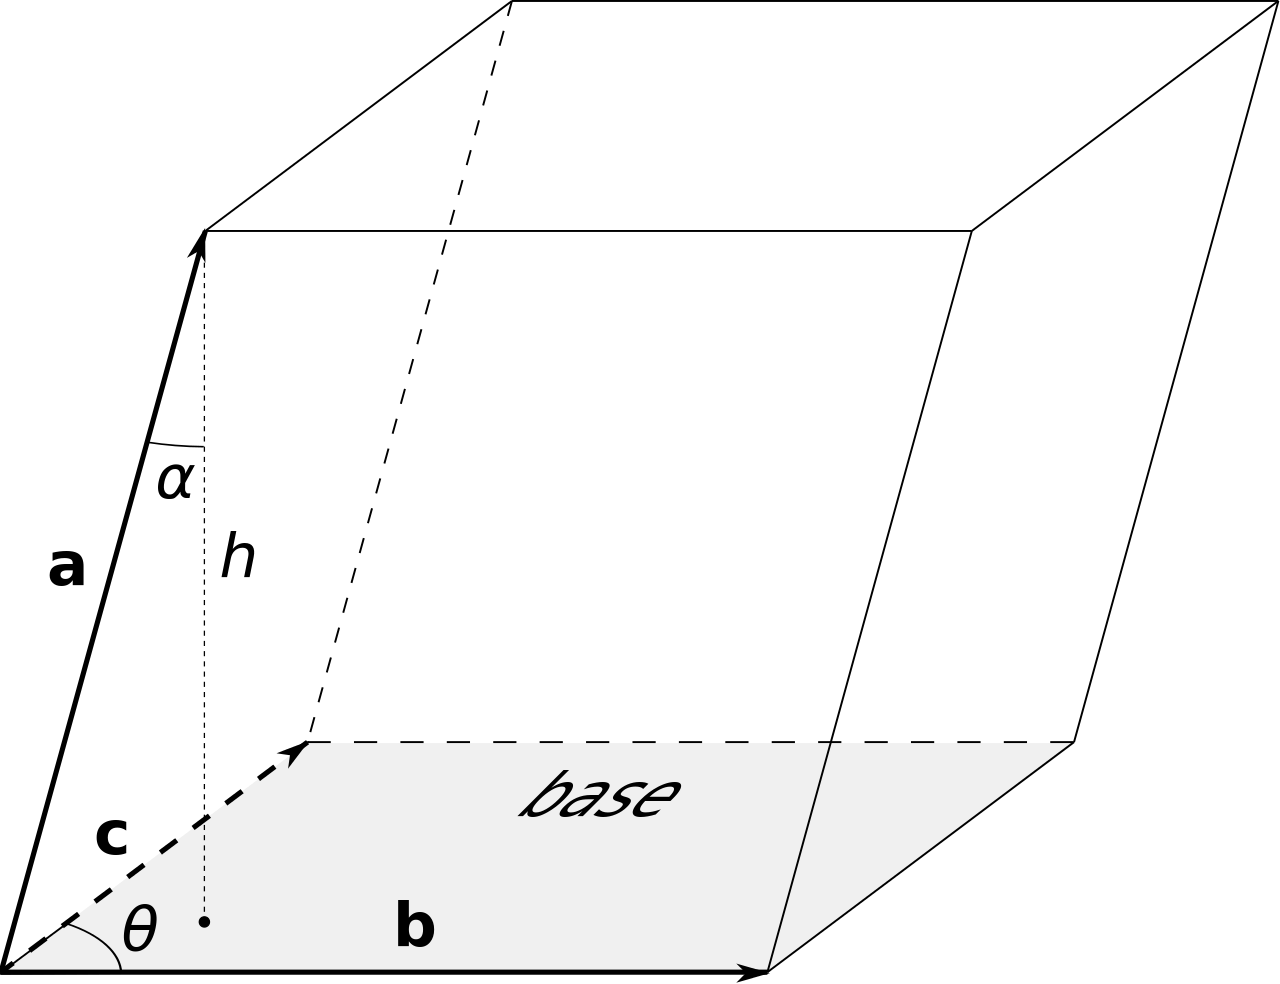
\includegraphics[height=120pt]{assets/Scalar_triple_product.png}
    \captionof{figure}{Scalar triple product}
\end{center}

The volume of this parallelepiped is
\[V = \boldsymbol a \cdot (\boldsymbol b \times \boldsymbol c) = \boldsymbol c \cdot (\boldsymbol a \times \boldsymbol b) = \boldsymbol b \cdot (\boldsymbol c \times \boldsymbol a).\]

Here,
\[\boldsymbol a \cdot (\boldsymbol b \times \boldsymbol c) = \boldsymbol a \cdot (b_i c_j \varepsilon_{ijk} \boldsymbol e_k) = b_i c_j a_k \varepsilon_{ijk},\]
\[\boldsymbol b \cdot (\boldsymbol c \times \boldsymbol a) = \boldsymbol b \cdot (c_i a_j \varepsilon_{ijk} \boldsymbol e_k) = c_i a_j b_k \varepsilon_{ijk},\]
\[\boldsymbol c \cdot (\boldsymbol a \times \boldsymbol b) = \boldsymbol c \cdot (a_i b_j \varepsilon_{ijk} \boldsymbol e_k) = a_i b_j c_k \varepsilon_{ijk},\]
where \(i\), \(j\) and \(k\) are all dumb indices (哑标).

We usually record \begin{align*}
    \begin{bmatrix} \boldsymbol a & \boldsymbol b & \boldsymbol c \end{bmatrix} & = \boldsymbol a \cdot (\boldsymbol b \times \boldsymbol c) = \boldsymbol c \cdot (\boldsymbol a \times \boldsymbol b) = \boldsymbol b \cdot (\boldsymbol c \times \boldsymbol a) \\
    & = \begin{vmatrix}
            a_1 & a_2 & a_3 \\
            b_1 & b_2 & b_3 \\
            c_1 & c_2 & c_3
    \end{vmatrix}.
\end{align*}

\section[Static equilibrium conditions 静力平衡条件]{Static equilibrium conditions (derived using virtual work)
(用虚功原理推导的)
静力平衡条件}\label{static-equilibrium-conditions-derived-using-virtual-work-ux7528ux865aux529fux539fux7406ux63a8ux5bfcux7684-ux9759ux529bux5e73ux8861ux6761ux4ef6}

In mechanics, there are two kinds of displacements (位移):

\begin{itemize}
\tightlist{}
\item real displacement 实位移
\item virtual displacement 虚位移
\end{itemize}

The static equilibrium conditions are:

\begin{itemize}
\tightlist{}
\item Resultant force 合力
    \[\sum_i \boldsymbol F_i = \boldsymbol 0\]
\item
    Resultant torque/moment 合力矩
    \[\sum_i \boldsymbol r_i \times \boldsymbol F_i = \sum_i \boldsymbol \tau_i = \boldsymbol 0\]
\end{itemize}

For a rigid body (刚体), there are 2 kinds of motion:

\begin{itemize}
\tightlist{}
\item translation 平动
\item rotation 转动
\end{itemize}

When calculating virtual work, we assume that we have 

\begin{itemize}
\tightlist{}
\item In translation: virtual displacement \(\delta \boldsymbol u_0\)
\item In rotation: virtual rotational angle \(\delta \boldsymbol \Theta\)
\end{itemize}

The resultant virtual displacement (总虚位移) is
\[\delta \boldsymbol u_i = \delta \boldsymbol u_0 + \delta \boldsymbol \Theta \times \boldsymbol r_i.\]

Virtual work is \begin{align*}
    \delta W & = \sum_i \boldsymbol F_i \cdot \delta \boldsymbol u_i \\
    & = \sum_i \left( \boldsymbol F_i \cdot \delta \boldsymbol u_0 \right) + \sum_i \left[ \boldsymbol F_i \cdot \left (\delta \boldsymbol \Theta \times \boldsymbol r_i \right) \right] \\
    & = \delta \boldsymbol u_0 \cdot \sum_i \boldsymbol F_i + \sum_i \left[ \delta \boldsymbol \Theta \cdot \left (\boldsymbol r_i \times \boldsymbol F_i \right) \right] \\
    & = \delta \boldsymbol u_0 \cdot \sum_i \boldsymbol F_i + \delta \boldsymbol \Theta \cdot \sum_i \left (\boldsymbol r_i \times \boldsymbol F_i \right).
\end{align*}

Because \(\delta \boldsymbol u_0\) and \(\delta \boldsymbol \Theta\) are
arbitrary (任意的,任取的), and work is positive definite
(功具有正定性), in equilibrium we have
\[\delta W = 0 \Rightarrow \left\{
    \begin{array}{ll}
        \delta \boldsymbol u_0 \cdot \sum_i \boldsymbol F_i = 0 & \Rightarrow  \sum_i \boldsymbol F_i = \boldsymbol 0
        \\[1.5ex]
        \delta \boldsymbol \Theta \cdot \sum_i \left (\boldsymbol r_i \times \boldsymbol F_i \right) = 0 & \Rightarrow  \sum_i \left (\boldsymbol r_i \times \boldsymbol F_i \right) = \boldsymbol 0.
    \end{array}
\right.\]

\chapter{2023/11/01}\label{20231101}

\emph{如果你对一个问题了解不深,但你仍去做科普,那么你很有可能造成误导的效果。}

\section{Tea leaf paradox
茶叶佯谬}\label{tea-leaf-paradox-ux8336ux53f6ux4f6fux8c2c}

When the fluid is stirred, stirring makes the primary flow (as shown in
the picture). It is easy to know that the surface of the water is a
paraboloid (抛物面), which is higher near the edge of the cup. Thus, the
pressure near the edge is greater than the center.

According to Bernoulli's principle, the greater the pressure, the less
the speed of flow.

Thus the centrifugal force is weaker near the bottom than higher up,
leading to a secondary flow (二次流) that goes outwards at the top, down
along the outer edge, inwards along the bottom, bringing the leaves to
the center, and then up again.

\begin{center}
    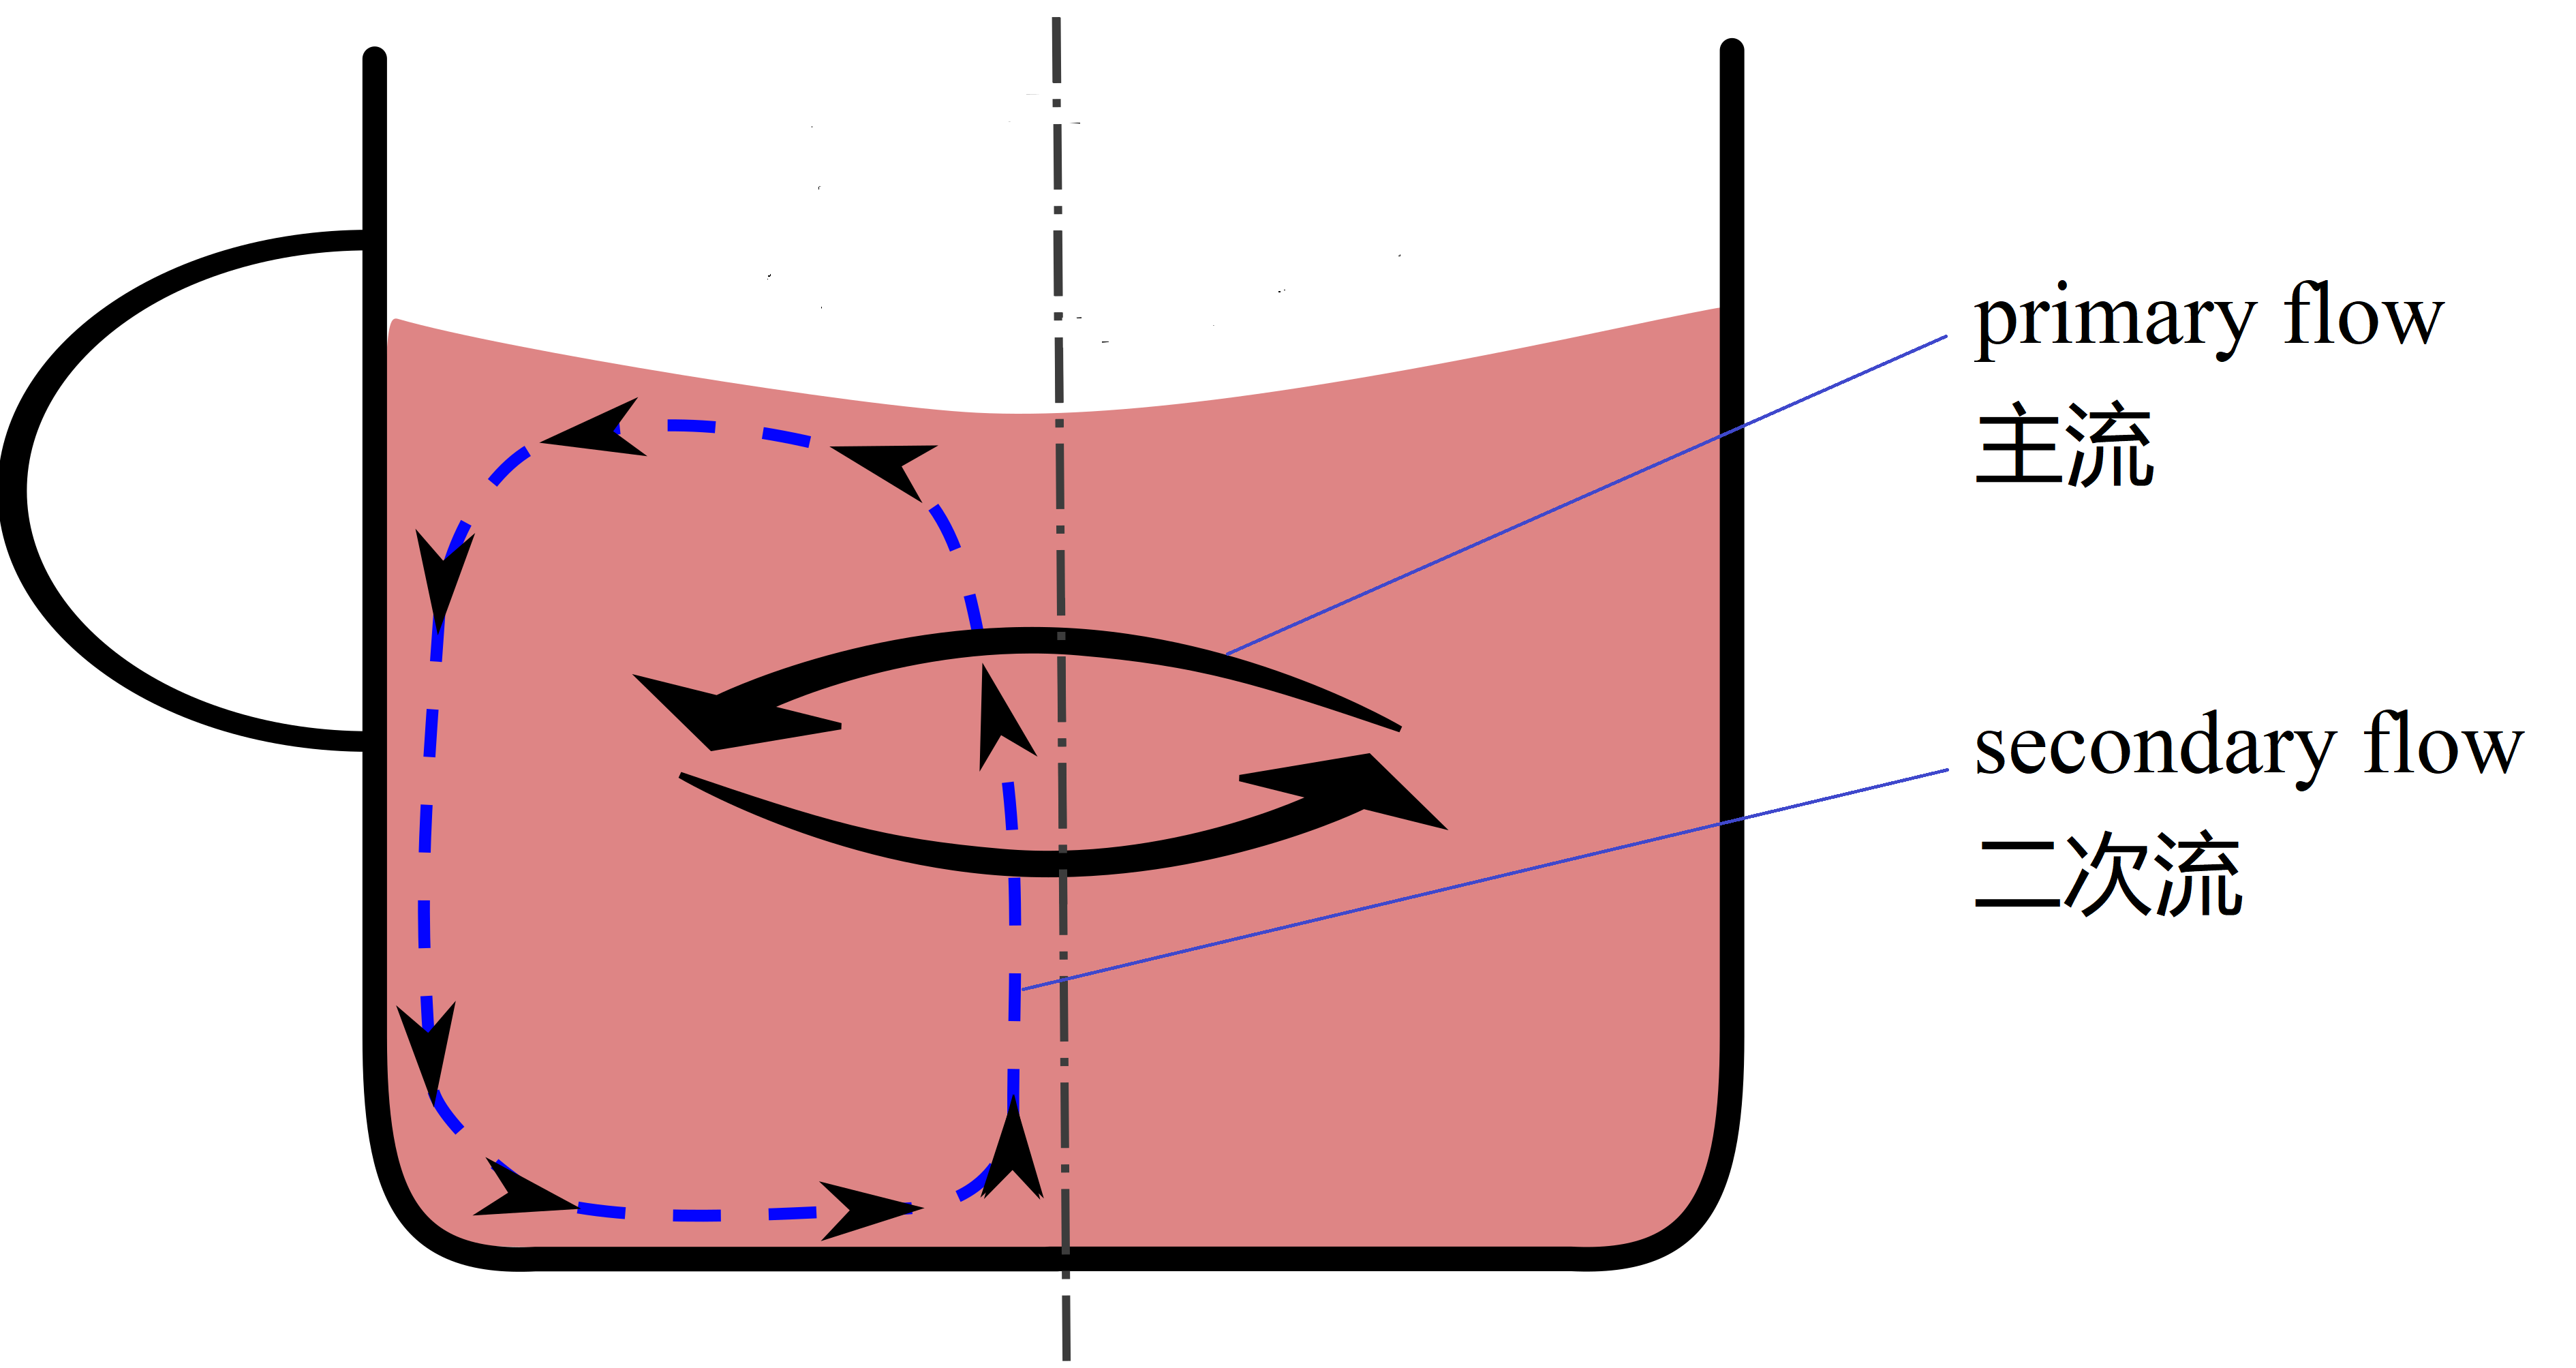
\includegraphics[height=100pt]{assets/Tea_leaf_paradox.png}
    \captionof{figure}{Primary and secondary flow in the tea leaf paradox}
\end{center}

\begin{quote}
作业:拜耳定律是什么?
\end{quote}

\section{Rotation system
旋转系统}\label{rotation-system-ux65cbux8f6cux7cfbux7edf}

\subsection*{(1) Special orthogonal group
特殊正交群}\label{special-orthogonal-group-ux7279ux6b8aux6b63ux4ea4ux7fa4}

The transformation between inertial frames \(S\) and \(S'\) (rotation by
an angle \(\theta\)) is \[\left\{
    \begin{array}{l}
        \hat i = \hat i' \cos \theta - \hat j' \sin \theta, \\
        \hat j = \hat i' \sin \theta + \hat j' \cos \theta.
    \end{array}
\right.\]

Put it in matrix form, and we get: \[\begin{pmatrix}
    \hat i \\
    \hat j
\end{pmatrix} =
\begin{pmatrix}
    \cos \theta & -\sin \theta \\
    \sin \theta & \cos \theta
\end{pmatrix}
\begin{pmatrix}
    \hat i' \\
    \hat j'
\end{pmatrix}.\]

Let \[\mathbf R(\theta) = 
\begin{pmatrix}
\cos \theta & -\sin \theta \\
\sin \theta & \cos \theta
\end{pmatrix},\] and we know that \(\mathbf R\) has the following
qualities:

\begin{enumerate}
\def\labelenumi{(\arabic{enumi})}
\item
  \(\det \mathbf R = 1.\) This means that \(\mathbf R\) is a
  \textbf{special orthogonal group (特殊正交群, SO)}, and one such group
  in dimension \(n\) is denoted \(\operatorname{SO}(n)\). In this case,
  \(\mathbf R\) is \(\operatorname{SO}(2)\) (二维特殊正交群).
\item
  \(\mathbf R^\mathrm{T}(\theta) = \mathbf R^{-1} (\theta).\) Here,
  \(\mathrm T\) is short for \textbf{transpose (转置)}, and \(-1\) for
  \textbf{inverse (逆)}.
\end{enumerate}

\[\mathbf R^\mathrm{T}(\theta) \mathbf R(\theta) = \mathbf R^{-1} (\theta) \mathbf R(\theta) = \mathbf I = \begin{pmatrix}
1 & 0 \\
0 & 1
\end{pmatrix}.\]

\begin{quote}
作业:什么是流形?
\end{quote}

A group has four kinds of properties:

\begin{enumerate}
\def\labelenumi{\arabic{enumi}.}
\setcounter{enumi}{1}
\item Closure 封闭性
\item Associative 结合性
\item Unitarity 幺正性
\item Inverse 有逆
\end{enumerate}

\begin{quote}
作业:阿贝尔群 (Abel Group) 是什么?

(满足可交换性的群,如旋转群
\(\mathbf R(\theta_2) \mathbf R(\theta_1) = \mathbf R(\theta_1) \mathbf R(\theta_2).\))
\end{quote}

\subsection*{(2) \(\operatorname U(1)\) Group ~
\(\operatorname U(1)\)
群}\label{operatorname-u1-group-operatorname-u1-ux7fa4}

Here \(\operatorname U(1)\) stands for ``unitarity (酉,幺正)''.

The form of the \(\operatorname U(1)\) group is
\[\operatorname U(\theta) = \mathrm e^{\mathrm i \theta} = \cos \theta + \mathrm i \sin \theta. \quad (*)\]

The conjugate (共轭) of \((*)\) is
\[\operatorname U^*(\theta) = \mathrm e^{- \mathrm i \theta} = \cos \theta - \mathrm i \sin \theta.\]

We can see that \(\operatorname{SO}(2)\) is an isomorphism (同构) of
\(\operatorname U(\theta)\):
\[\operatorname{SO}(2) \cong \operatorname U(\theta).\]

\begin{quote}
作业:什么是同构?

群 \(G\) 与 \(G'\) 是同构的,如果存在一个双射 \(\varphi: G \to G'\)
,满足 \(\varphi(xy) = \varphi(x)\varphi(y)\) ,其中 \(x, y \in G\)
。双射 \(\varphi\) 称为群 \(G\) 和 \(G'\) 的一个同构,记为
\(G \cong G'.\)
\end{quote}

\section[Acceleration in polar coordinates 极坐标加速度]{Acceleration decomposition in polar coordinates 极坐标下的加速度分解}\label{acceleration-decomposition-in-polar-coordinates-ux6781ux5750ux6807ux4e0bux7684ux52a0ux901fux5ea6ux5206ux89e3}

The transformation between inertial frames \(S'\) (rotation by an angle
\(\theta\)) and \(S\) is \[\left\{
    \begin{array}{l}
        \hat i' = \cos \theta \hat i + \sin \theta \hat j, \\
        \hat j' = - \sin \theta \hat i + \cos \theta \hat j.
    \end{array}
\right.\]

Take the derivative of the equations above and we get \[\left\{
    \begin{array}{l}
        \dfrac{\mathrm d \hat i'}{\mathrm d t} = (- \sin \theta \hat i + \cos \theta \hat j) \dot \theta = \dot \theta \hat j', \\
        \dfrac{\mathrm d \hat j'}{\mathrm d t} = (- \cos \theta \hat i - \sin \theta \hat j) \dot \theta = - \dot \theta \hat i'.
    \end{array}
\right.\]

Thus the radius vector is \[\boldsymbol r = r \hat i';\]

The velocity is
\[\boldsymbol v' = \dfrac{\mathrm d \boldsymbol r}{\mathrm dt} = \dfrac{\mathrm dr}{\mathrm dt} \hat i' + r \dfrac{\mathrm d \hat i'}{\mathrm dt} = \dfrac{\mathrm dr}{\mathrm dt} \hat i' + r \dot \theta \hat j' = v_r \hat i' + v_\theta \hat j';\]

The acceleration is \begin{align*}
    \boldsymbol a & = \dfrac{\mathrm d \boldsymbol v}{\mathrm dt} = \dfrac{\mathrm d}{\mathrm dt} \left( \dfrac{\mathrm dr}{\mathrm dt} \hat i' + r \dot \theta \hat j' \right) \\
    & = \dfrac{\mathrm d^2 r}{\mathrm dt^2} \hat i' + \dfrac{\mathrm dr}{\mathrm dt} \dot \theta \hat j' + \dfrac{\mathrm dr}{\mathrm dt} \dot \theta \hat j' +  r \ddot \theta \hat j' +  r \dot \theta (- \dot \theta \hat i') \\
    & = (\ddot r - r \dot \theta^2) \hat i' + (r \ddot  \theta + 2 \dot r \dot \theta) \hat j'.
\end{align*}

\emph{整理者附:这个推导好像跟科氏加速度没有半毛钱关系啊\ldots\ldots{}}

\emph{注:赵老师上课说的所谓``科氏加速度''指的是
\(2 \dot r \dot \theta \hat j'\) 一项}

\section{Transport theorem in a rotation system
旋转系的输运定理}\label{transport-theorem-in-a-rotation-system-ux65cbux8f6cux7cfbux7684ux8f93ux8fd0ux5b9aux7406}

\subsection*{(1) Derivation 推导}\label{derivation-ux63a8ux5bfc-1}

In a rotation system, we have the base factors \(\hat i'\) and
\(\hat j'\), we have
\[\dfrac{\mathrm d \hat r}{\mathrm dt} = \boldsymbol \omega \times \hat r,\]
where \(\boldsymbol \omega = (0, 0, \omega),\) and
\(\hat r = (\hat i', \hat j', \hat k')\).

Take the derivatives of \(\hat i'\) and \(\hat j'\), and we acquire
\[\dfrac{\mathrm d \hat i'}{\mathrm dt} = 
    \begin{vmatrix}
        \hat i' & \hat j' & \hat k' \\
        0 & 0 & \omega \\
        1 & 0 & 0
    \end{vmatrix}
= \omega \hat j';\]
\[\dfrac{\mathrm d \hat j'}{\mathrm dt} = \begin{vmatrix}
\hat i' & \hat j' & \hat k' \\
0 & 0 & \omega \\
0 & 1 & 0
\end{vmatrix}
= - \omega \hat i'.\]

Let \(\boldsymbol f = f_x \hat i' + f_y \hat j' + f_z \hat k'\), and
\begin{align*}
    \dfrac{\mathrm d \boldsymbol f}{\mathrm dt} & = \left( \dfrac{\mathrm df_x}{\mathrm dt} \right)_r \hat i' + \left( \dfrac{\mathrm df_y}{\mathrm dt} \right)_r \hat j' + \left( \dfrac{\mathrm df_z}{\mathrm dt} \right)_r \hat k' + f_x \dfrac{\mathrm d \hat i'}{\mathrm dt} + f_y \dfrac{\mathrm d \hat j'}{\mathrm dt} + f_z \dfrac{\mathrm d \hat k'}{\mathrm dt} \\
    & = \left( \dfrac{\mathrm d \boldsymbol f}{\mathrm dt} \right)_r + f_x \boldsymbol \omega \times \hat i' + f_y \boldsymbol \omega \times \hat j' + f_z \boldsymbol \omega \times \hat k' \\
    & = \left[ \left( \dfrac{\mathrm d}{\mathrm dt}\right)_r + \boldsymbol \omega \times \right] \boldsymbol f.
\end{align*}

Let \(\boldsymbol f = \boldsymbol r\), and we get
\[\boldsymbol v = \dfrac{\mathrm d \boldsymbol r}{\mathrm dt} = \left( \dfrac{\mathrm d \boldsymbol r}{\mathrm dt}\right)_r + \boldsymbol \omega;\]
\begin{align*}
    \boldsymbol a & = \dfrac{\mathrm d \boldsymbol v}{\mathrm dt} \\
    & = \left[ \left( \dfrac{\mathrm d}{\mathrm dt}\right)_r + \boldsymbol \omega \times \right] \left[ \left( \dfrac{\mathrm d \boldsymbol r}{\mathrm dt}\right)_r + \boldsymbol \omega \times \boldsymbol r \right] \\
    & = \left( \dfrac{\mathrm d^2 \boldsymbol r}{\mathrm dt^2}\right)_r + \left( \dfrac{\mathrm d \boldsymbol \omega}{\mathrm dt}\right)_r \times \boldsymbol r + 2 \boldsymbol \omega \times \left( \dfrac{\mathrm d \boldsymbol r}{\mathrm dt}\right)_r + \boldsymbol \omega \times (\boldsymbol \omega \times \boldsymbol r).
\end{align*}

\subsection*{(2) Example: Euler's equations in rigid body dynamics
刚体运动的欧拉方程}\label{example-eulers-equations-in-rigid-body-dynamics-ux521aux4f53ux8fd0ux52a8ux7684ux6b27ux62c9ux65b9ux7a0b}

Basically, if we have the angular momentum \(\boldsymbol L\), angular
velocity \(\boldsymbol \omega\) and moment of inertia tensor (惯性张量)
\(\mathbf I\), we will have
\[\boldsymbol L = \mathbf I \cdot \boldsymbol \omega.\]

According to the Angular Momentum Theorem, we have
\[\dfrac{\mathrm d \boldsymbol L}{\mathrm dt} = \boldsymbol M,\] where
\(\boldsymbol M\) is the external torque (外力矩). From this, we can get
\[\left[ \dfrac{\mathrm d (\mathbf I \boldsymbol \omega)}{\mathrm dt}\right]_r + \boldsymbol \omega \times (\mathbf I \boldsymbol \omega) = \boldsymbol M.\]

Because \(\mathbf I\) is a constant, we have
\[\mathbf I \left( \dfrac{\mathrm d \boldsymbol \omega}{\mathrm dt} \right)_r + \begin{vmatrix}
    \hat i & \hat j & \hat k \\
    \omega_1 & \omega_2 & \omega_3 \\
    \mathrm I_{11} \omega_1 & \mathrm I_{22} \omega_2 & \mathrm I_{33} \omega_3 \\
\end{vmatrix} =\begin{pmatrix}
    M_1 \\ M_2 \\ M_3
\end{pmatrix}.\]

In orthogonal principal axes of inertia coordinates
(惯性坐标的正交主轴), the equations become \begin{align*}
    \mathrm I_{11} \dfrac{\mathrm d \boldsymbol \omega_1}{\mathrm dt} + (\mathrm I_{33} - \mathrm I_{22}) \omega_2 \omega_3 & = M_1; \\
    \mathrm I_{22} \dfrac{\mathrm d \boldsymbol \omega_2}{\mathrm dt} + (\mathrm I_{11} - \mathrm I_{33}) \omega_1 \omega_3 & = M_2; \\
    \mathrm I_{33} \dfrac{\mathrm d \boldsymbol \omega_3}{\mathrm dt} + (\mathrm I_{22} - \mathrm I_{11}) \omega_1 \omega_2 & = M_3.
\end{align*}

\chapter{2023/11/06}\label{20231106}

\section{Real and virtual displacement
实位移和虚位移}\label{real-and-virtual-displacement-ux5b9eux4f4dux79fbux548cux865aux4f4dux79fb}

\emph{见附录B。}

\section{Something about tensors
一些关于张量的讨论}\label{something-about-tensors-ux4e00ux4e9bux5173ux4e8eux5f20ux91cfux7684ux8ba8ux8bba}

\subsection*{(1) Projection tensor
投影张量}\label{projection-tensor-ux6295ux5f71ux5f20ux91cf}

\begin{center}
    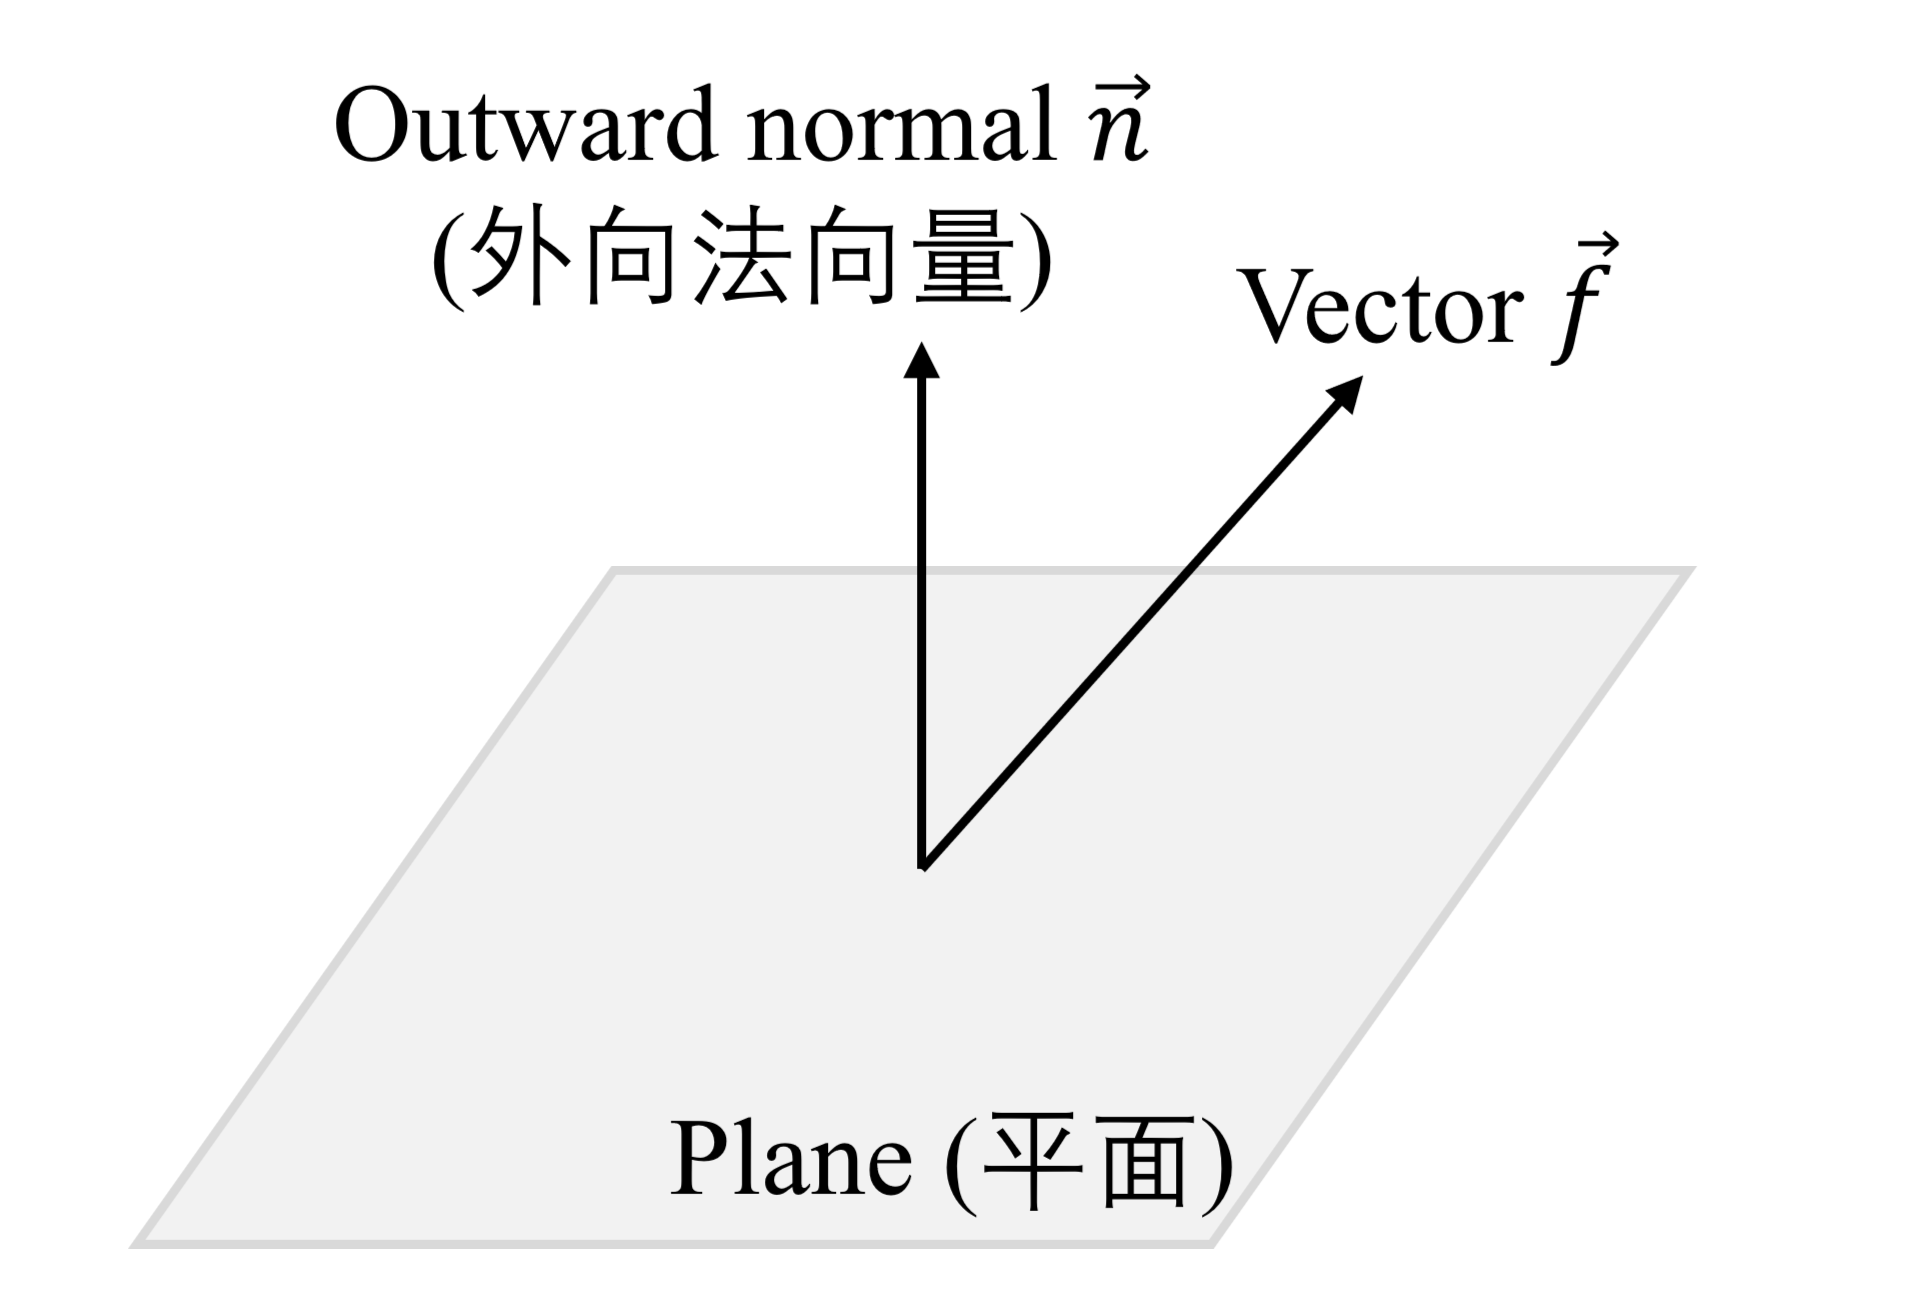
\includegraphics[height=120pt]{assets/Projection_Tensor.png}
    \captionof{figure}{Projection tensor}
\end{center}

Fig 15.1 shows a plain with an outward normal \(\boldsymbol n\)
(\(\boldsymbol n \cdot \boldsymbol n = \boldsymbol n^2 = 1\)), and we
can get the projection of the vector \(\boldsymbol f\):
\[\boldsymbol f_\perp = (\boldsymbol f \cdot \boldsymbol n) \boldsymbol n = \boldsymbol f \cdot (\boldsymbol n \otimes \boldsymbol n). \quad (*)\]

Thus we can get
\[\boldsymbol f_{/\!/} = \boldsymbol f - \boldsymbol f_\perp = \boldsymbol f - \boldsymbol f \cdot (\boldsymbol n \otimes \boldsymbol n) = \boldsymbol f \cdot (\mathbf e - \boldsymbol n \otimes \boldsymbol n).\]

Let \[\mathbf P = \mathbf e - \boldsymbol n \otimes \boldsymbol n,\] and
we call \(\mathbf P\) the \textbf{projection tensor of rank 2
(二阶投影张量)}. An interesting piece of quality of \(\mathbf P\) is:
\begin{align*}
    \mathbf P^2 & = (\mathbf e - \boldsymbol n \otimes \boldsymbol n)^2 \\
    & = \mathbf e^2 - 2 \boldsymbol n \otimes \boldsymbol n + (\boldsymbol n \otimes \boldsymbol n) \cdot (\boldsymbol n \otimes \boldsymbol n) \\
    & = \mathbf e - 2 \boldsymbol n \otimes \boldsymbol n + \boldsymbol n \otimes (\boldsymbol n \cdot \boldsymbol n) \otimes \boldsymbol n \\
    & = \mathbf e - 2 \boldsymbol n \otimes \boldsymbol n + \boldsymbol n \otimes \boldsymbol n\\
    & = \mathbf e - \boldsymbol n \otimes \boldsymbol n \\
    & = \mathbf P.
\end{align*}

Note:

\begin{enumerate}
\def\labelenumi{\arabic{enumi}.}
\tightlist{}
\item Above, \(\otimes\) stands for tensor product (张量积).
\item 
  The proof of \((*)\): \begin{align*}
   \boldsymbol f \cdot (\boldsymbol n \otimes \boldsymbol n) & = (f_k \boldsymbol e_k) \cdot (n_i n_j \boldsymbol e_i \otimes \boldsymbol e_j) \\
   & = (f_k \boldsymbol e_k \cdot n_i n_j \boldsymbol e_i) \boldsymbol e_j \\
   & = f_k n_i n_j \delta_{ik} \boldsymbol e_j \\
   & = f_i n_i n_j \boldsymbol e_j \\
   & = (\boldsymbol f \cdot \boldsymbol n) \boldsymbol n.
  \end{align*}
\end{enumerate}

\subsection*{(2) Moment of inertia tensor 惯性张量
\(\boldsymbol I\)}\label{moment-of-inertia-tensor-ux60efux6027ux5f20ux91cf-boldsymbol-i}

Angular momentum is \begin{align*}
    \boldsymbol L & = \int \boldsymbol r \times \mathrm d \boldsymbol p \\
    & = \int \boldsymbol r \times \rho \boldsymbol v \mathrm dV \\
    & = \rho \int \boldsymbol r_i \times (\boldsymbol \omega \times \boldsymbol r_i) \mathrm dV \\
\end{align*}
\begin{align*}
    & = \rho \int [\boldsymbol \omega (\boldsymbol r_i \cdot \boldsymbol r_i) - \boldsymbol r_i (\boldsymbol r_i \cdot \boldsymbol \omega)] \mathrm dV \\
    & = \rho \int [\boldsymbol \omega r_i^2 - (\boldsymbol r_i \otimes \boldsymbol r_i) \boldsymbol \omega] \mathrm dV \\
    & = \left[ \rho \int (r_i^2 \mathbf e - \boldsymbol r_i \otimes \boldsymbol r_i) \mathrm dV \right] \cdot \boldsymbol \omega.
\end{align*}

From \(\boldsymbol L = \boldsymbol I \cdot \boldsymbol \omega\), we can
see that
\[\boldsymbol I = \rho \int (r_i^2 \mathbf e - \boldsymbol r_i \otimes \boldsymbol r_i) \mathrm dV,\]
which, written in index form, is
\[I_{ij} = \rho \int \left[ (x^2 + y^2 + z^2) \delta_{ij} - x_ix_j \right]\mathrm dV.\]

Written in Cartesian coordinates are: \[\left\{
    \begin{array}{l}
        \displaystyle I_{xx} = \rho \int \left( y^2 + z^2 \right) \mathrm dV, \\
        \displaystyle I_{yy} = \rho \int \left( x^2 + z^2 \right) \mathrm dV, \\
        \displaystyle I_{zz} = \rho \int \left( x^2 + y^2 \right) \mathrm dV, \\
    \end{array}
\right.
\quad \text{and} \quad
\left\{
    \begin{array}{l}
        \displaystyle I_{xy} = \rho \int xy \mathrm dV, \\
        \displaystyle I_{yz} = \rho \int yz \mathrm dV, \\
        \displaystyle I_{xz} = \rho \int xz \mathrm dV. \\
    \end{array}
\right.\]

\section[The conservation of the LRL vector 拉普拉斯--龙格--楞次矢量守恒]{Two methods of deriving the conservation of the Laplace--Runge--Lenz (LRL) vector under a central force field that follows the inverse square law 两种推导平方反比有心力场下拉普拉斯--龙格--楞次矢量守恒的方法}\label{two-methods-of-deriving-the-conservation-of-the-laplacerungelenz-lrl-vector-under-a-central-force-field-that-follows-the-inverse-square-law-ux4e24ux79cdux63a8ux5bfcux5e73ux65b9ux53cdux6bd4ux6709ux5fc3ux529bux573aux4e0bux62c9ux666eux62c9ux65af-ux9f99ux683c-ux695eux6b21ux77e2ux91cfux5b88ux6052ux7684ux65b9ux6cd5}

The Laplace--Runge--Lenz (LRL) vector \(\boldsymbol A\) is
\[\boldsymbol A = \boldsymbol p \times \boldsymbol L - m \kappa \hat {\boldsymbol r}.\]

The following discussion is set under this specific central force field
(有心力场) \(U(r)\): \[U(r) = - {GMm \over r} = - {\kappa \over r}.\]

In this central force field, there are three conserved qualities
(守恒量):

\begin{itemize}
\tightlist{}
\item
  \(\displaystyle E = {p^2 \over 2m} - {\kappa \over r}\)
\item 
  \(\displaystyle \boldsymbol L = \boldsymbol r \times \boldsymbol p\)
\item
  \(\displaystyle \boldsymbol A = \boldsymbol p \times \boldsymbol L - m \kappa \hat {\boldsymbol r}\)
\end{itemize}

\subsection*{(1) Method 1}\label{method-1}

\[\boldsymbol A = \boldsymbol p \times \boldsymbol L - m \kappa \hat {\boldsymbol r}.\]

\[\dfrac{\mathrm d \boldsymbol A}{\mathrm dt} = \dot {\boldsymbol p} \times \boldsymbol L + \boldsymbol p \times \dot {\boldsymbol L} - m \kappa \dfrac{\mathrm d \hat {\boldsymbol r}}{\mathrm dt}.\]

Here, \(\boldsymbol L\) is conserved, and thus
\(\dot {\boldsymbol L} = \boldsymbol 0.\)

According to Newton's laws of motion, we have
\[\dot {\boldsymbol p} = \boldsymbol f = - {\kappa \over r^2} \hat {\boldsymbol r}.\]

Using transport theorem, we know that
\[\dfrac{\mathrm d \hat {\boldsymbol r}}{\mathrm dt} = \left( \dfrac{\mathrm d \hat {\boldsymbol r}}{\mathrm dt} \right)_r + \boldsymbol \omega \times \hat {\boldsymbol r} = \boldsymbol \omega \times \hat {\boldsymbol r}.\]

Thus, \begin{align*}
    \dfrac{\mathrm d \boldsymbol A}{\mathrm dt} & = \left(- {\kappa \over r^2} \hat {\boldsymbol r} \right) \times m r^2 \boldsymbol \omega - m \kappa (\boldsymbol \omega \times \hat {\boldsymbol r}) \\
    & = - m \kappa \hat {\boldsymbol r} \times\boldsymbol \omega - m \kappa \boldsymbol \omega \times \hat {\boldsymbol r} \\
    & = \boldsymbol 0.
\end{align*}

\subsection*{(2) Method 2}\label{method-2}

\begin{align*}
    \dfrac{\mathrm d \boldsymbol A}{\mathrm dt} & = \dot {\boldsymbol p} \times \boldsymbol L + \boldsymbol p \times \dot {\boldsymbol L} - m \kappa \dfrac{\mathrm d \hat {\boldsymbol r}}{\mathrm dt} \\
    & = \left(- {\kappa \over r^2} \hat {\boldsymbol r} \right) \times \left( \boldsymbol r \times m {\mathrm d \boldsymbol r \over \mathrm dt} \right) - m \kappa {1 \over r} {\mathrm d \boldsymbol r \over \mathrm dt} +a {m \kappa \over r^2} \boldsymbol r {\mathrm dr \over \mathrm dt} \\
    & = - {m \kappa \over r^3} \left[ \boldsymbol r \times \left( \boldsymbol r \times {\mathrm d \boldsymbol r \over \mathrm dt} \right) + r^2 {\mathrm d \boldsymbol r \over \mathrm dt} - \boldsymbol r r {\mathrm d r \over \mathrm dt} \right]\\
    & = - {m \kappa \over r^3}\left[ \boldsymbol r \left( \boldsymbol r \cdot {\mathrm d \boldsymbol r \over \mathrm dt} \right) - r^2 {\mathrm d \boldsymbol r \over \mathrm dt} + r^2 {\mathrm d \boldsymbol r \over \mathrm dt} - \boldsymbol r r {\mathrm d r \over \mathrm dt} \right]\\
    & = \boldsymbol 0.
\end{align*}

\chapter{2023/11/08}\label{20231108}

\textbf{\emph{划重点!划重点!}}

\textbf{\emph{本次课上,赵爹披露重大新闻,引起全班轰动!}}

\textbf{\emph{据悉,赵爹曾四次受到剑桥大学出版社邀请,将《力学讲义》译成英文出版!!他没有去!!}}

\section{Galilean invariance
伽利略不变性}\label{galilean-invariance-ux4f3dux5229ux7565ux4e0dux53d8ux6027}

\subsection*{(1) Basic forms}\label{basic-forms}

The basic foundation of Galilean invariance is \[\left\{
    \begin{array}{l}
        \boldsymbol r' = \boldsymbol r - \boldsymbol Vt, \\
        t' = t,
    \end{array}
\right.\] where \(\boldsymbol V\) is a constant vector (常矢量).

According to this foundation, we can know:
\[{\partial \over \partial t} = {\partial \over \partial t'}{\partial t' \over \partial t} + {\partial \over \partial \boldsymbol r'}{\partial \boldsymbol r' \over \partial t} = {\partial \over \partial t'} - \boldsymbol V \cdot \nabla';\]
\[{\partial \over \partial \boldsymbol r} = \nabla = {\partial \over \partial \boldsymbol r'}{\partial \boldsymbol r' \over \partial \boldsymbol r} = \nabla' \cdot \mathbf I = \nabla'.\]

\subsection*{(2) Three principal invariants of second-order tensors
二阶张量的三个主不变量}\label{three-principal-invariants-of-second-order-tensors-ux4e8cux9636ux5f20ux91cfux7684ux4e09ux4e2aux4e3bux4e0dux53d8ux91cf}

\begin{quote}
\emph{此话题似乎由课上一位同学指出的赵爹的一个拼写错误引起,和上下文没有大的关系。故译者另附表格,希望大家不要弄混:}
    \begin{center}
        \begin{tabular}{|c|l|}
            \hline
            \textbf{Word} & \textbf{Definition} \\
            \hline
            invariant & \textit{n.} 不变量; \textit{adj.} 不变的 \\
            \hline
            invariance & \textit{n.} 不变性 \\
            \hline
        \end{tabular}
    \end{center}
\end{quote}

Suppose we have a matrix \[\mathbf A = 
\begin{bmatrix}
    A_{11} & A_{12} &A_{13} \\
    A_{21} & A_{22} &A_{23} \\
    A_{31} & A_{32} &A_{33}
\end{bmatrix}.\]

If \(\mathbf A \cdot \boldsymbol v = \lambda \boldsymbol v\), then we
call \(\boldsymbol v\) the \textbf{eigenvector (特征矢量,本征矢量)} of
the linear transformation \(\mathbf A\), and \(\lambda\) the
\textbf{eigenvalue (特征值,本征值)} of \(\mathbf A\).

From this, we have
\[\mathbf A \cdot \boldsymbol v - \lambda \boldsymbol v = \boldsymbol 0,\]
and thus
\[(\mathbf A - \lambda \mathbf e) \cdot \boldsymbol v = \boldsymbol 0,\]
which is a homogeneous (齐次的) equation. In order for this equation to
have a non-trivial solution (非平凡解), we need to have
\[\det (\mathbf A - \lambda \mathbf e) = 0.\] That is, \[\begin{vmatrix}
    A_{11} - \lambda & A_{12} & A_{13} \\
    A_{21} & A_{22} - \lambda & A_{23} \\
    A_{31} & A_{32} & A_{33} - \lambda 
\end{vmatrix} = 0,\] \begin{align*}
    (A_{11} - \lambda)(A_{22} - \lambda)(A_{33} - \lambda) + A_{12}A_{23}A_{31} + A_{13}A_{21}A_{32} & \\
    - (A_{11} - \lambda)A_{23}A_{32} - A_{13}(A_{22} - \lambda)A_{31} - A_{12}A_{21}(A_{33} - \lambda) & = 0.
\end{align*}

Arrange this formula, and we get
\[\lambda ^3 - I_1 \lambda ^2 + I_2 \lambda - I_3 = 0,\] in which
\begin{align*}
    I_1 & = \operatorname{tr} \mathbf{A} = A_{11} + A_{22} + A_{33} = \lambda_1 + \lambda_2 + \lambda_3, \\
    I_2 & = \frac{1}{2} \left[ (\operatorname{tr} \mathbf{A})^2 - \operatorname{tr} \left( \mathbf{A}^2 \right) \right] \\
    & = A_{11} A_{22} + A_{22} A_{33} + A_{11} A_{33} - A_{12} A_{21} - A_{23} A_{32} - A_{13} A_{31} \\ & = \lambda_1 \lambda_2 + \lambda_1 \lambda_3 + \lambda_2 \lambda_3, \\
    I_3 & = \det (\mathbf{A}) \\ & = - A_{13} A_{22} A_{31} + A_{12} A_{23} A_{31} + A_{13} A_{21} A_{32} \\ & \quad - A_{11} A_{23} A_{32} - A_{12} A_{21} A_{33} +   A_{11} A_{22} A_{33} \\ & = \lambda_1 \lambda_2 \lambda_3.
\end{align*}

\subsection*{(3) The Galilean Invariance in the Navier-Stokes
equations
纳维-斯托克斯方程的伽利略不变性}\label{the-galilean-invariance-in-the-navier-stokes-equations-ux7eb3ux7ef4-ux65afux6258ux514bux65afux65b9ux7a0bux7684ux4f3dux5229ux7565ux4e0dux53d8ux6027}

The Navier-Stokes equations is
\[ {\partial \boldsymbol v \over \partial t} +(\boldsymbol v \cdot \nabla) \boldsymbol v = - {1 \over \rho} \nabla p + \mu \nabla^2 \boldsymbol v + \boldsymbol g.\]

Put it in a Galilean transformation, and we can get \begin{align*}
    \text{LHS} & = \left( {\partial \over \partial t'} - \boldsymbol V \cdot \nabla' \right)(\boldsymbol v' + \boldsymbol V) + [(\boldsymbol v' + \boldsymbol V) \cdot \nabla'](\boldsymbol v' + \boldsymbol V) \\
    & = {\partial \boldsymbol v' \over \partial t} + \boldsymbol 0 - (\boldsymbol V \cdot \nabla') \boldsymbol v' - \boldsymbol 0 + (\boldsymbol v' \cdot \nabla') \boldsymbol v' + (\boldsymbol V \cdot \nabla') \boldsymbol v' \\
    & = {\partial \boldsymbol v' \over \partial t} + (\boldsymbol v' \cdot \nabla') \boldsymbol v'; \\
    \text{RHS} & = - {1 \over \rho} \nabla' \left( p + {1 \over 2} \rho V^2 \right) + \mu \nabla'^2 (\boldsymbol v' + \boldsymbol V) + \boldsymbol g \\
    & = - {1 \over \rho} \nabla' p + \mu \nabla'^2 \boldsymbol v' + \boldsymbol g. \\
\end{align*}

When \(\boldsymbol g\) conforms to the Galilean invariance, the
Navier-Stokes equations shall conform to the Galilean invariance.

\section{Square-Cube law (1638)
平方-立方定律}\label{square-cube-law-1638-ux5e73ux65b9-ux7acbux65b9ux5b9aux5f8b}

Take \(L\) as the characteristic value (特征尺度), and the area
\(A \sim L^2\), whereas the volume \(V \sim L^3\), proportional to the
weight. Consequently, we have \[{V \over A} \sim L.\]

For the full story, please refer to the ``Philosophy of Science''
section.

\section{Virial Theorem
位力定理}\label{virial-theorem-ux4f4dux529bux5b9aux7406}

\emph{杨振宁:不会凑就不要做理论物理研究}

The kinetic energy is
\[T = \sum_i {1 \over 2}m_i v_i^2 = \sum_i {1 \over 2}m_i \boldsymbol v_i \cdot \boldsymbol v_i.\]

Take the derivative of \(T\) with respect to \(\boldsymbol v\), we get
\begin{align*}
    {\partial T \over \partial \boldsymbol v} & = \sum_i {1 \over 2} m_i {\partial \over \partial \boldsymbol v}(\boldsymbol v_i \cdot \boldsymbol v_i) \\
    & = \sum_i {1 \over 2} m_i (\mathbf I \cdot \boldsymbol v_i + \boldsymbol v_i \cdot \mathbf I) \\
    & = \sum_i {1 \over 2} m_i \cdot 2 \boldsymbol v_i = \sum_i m_i \boldsymbol v_i = \boldsymbol p.
\end{align*}

Also, we have \begin{align*}
    2T & = \sum_i m_i \boldsymbol v_i \cdot \boldsymbol v_i \\
    & = \sum_i \boldsymbol p_i \cdot \boldsymbol v_i \\
    & = \sum_i \boldsymbol p_i \cdot {\mathrm d \boldsymbol r_i \over \mathrm dt} \\
    & = {\mathrm d \over \mathrm dt} \sum_i \boldsymbol p_i \cdot \boldsymbol r_i - \sum_i {\mathrm d \boldsymbol p_i \over \mathrm dt} \cdot \boldsymbol r_i \\
    & = {\mathrm d \over \mathrm dt} \sum_i \boldsymbol p_i \cdot \boldsymbol r_i - \sum_i \underset{\text{位}}{\underline{\boldsymbol r_i}} \cdot \underset{\text{力}}{\underline{\boldsymbol F_i}}. \quad(*)
\end{align*}

According to definition, the average of \(g(t)\) over a period of time
(from \(0\) to \(\tau\)) can be written as follows:
\[\left \langle g(t) \right \rangle_\tau = \frac{1} \tau \int_0^\tau g(t) \mathrm dt.\]

Assuming that $g(t) = \dfrac{\mathrm d G(t)}{\mathrm dt}$, we have \[\left \langle g(t) \right \rangle_\tau = \frac{1} \tau \int_0^\tau g(t) \mathrm dt = \frac{1}{\tau} \int_{G(0)}^{G(\tau)} \mathrm dG = \frac{G(\tau) - G(0)}{\tau},\] and, if \(G\) is a bounded function (有界函数), when \(\tau \to + \infty\), we have \[\left \langle g(t) \right \rangle_\tau = \lim_{\tau \to + \infty} \frac{1} \tau \int_0^\tau g(t) \mathrm dt = \lim_{\tau \to + \infty} \frac{1}{\tau} \int_{G(0)}^{G(\tau)} \mathrm dG = \lim_{\tau \to + \infty} \frac{G(\tau) - G(0)}{\tau} = 0.\]

In the case of bounded movement (有界运动),
\(\boldsymbol p_i \cdot \boldsymbol r_i\) is bounded as well, and when we take the average of \((*)\) over time, we can get that \[\left \langle {\mathrm d \over \mathrm dt} \sum_i \boldsymbol p_i \cdot \boldsymbol r_i \right \rangle_\tau = \lim_{\tau \to + \infty} \frac{\boldsymbol p_i(\tau) \cdot \boldsymbol r_i(\tau) - \boldsymbol p_i(0) \cdot \boldsymbol r_i(0)}{\tau} = 0,\]
and thus
\[\left \langle 2T \right \rangle_\tau = - \left \langle \sum_i \boldsymbol r_i \cdot \boldsymbol F_i \right \rangle_\tau = - \sum_i \left \langle \boldsymbol r_i \cdot \boldsymbol F_i \right \rangle_\tau.\]

This brings us to Virial theorem:
\[\left \langle T \right \rangle = - {1 \over 2} \sum_i \left \langle \boldsymbol r_i \cdot \boldsymbol F_i \right \rangle,\]
where \(T\) is the total kinetic energy of the particles,
\(\boldsymbol F_i\) represents the force on the \(i\) th particle, which
is located at position \(\boldsymbol r_i\), and angle brackets
\(\langle \rangle\) represent the average over time of the enclosed quantity.

\chapter{2023/11/13}\label{20231113}

\section{A further derivation of the Virial theorem 位力定理的
更深入推导}\label{a-further-ux66f4ux6df1ux5165ux63a8ux5bfc}

\subsection*{(1) Euler's homogeneous function theorem
欧拉齐次函数定理}\label{eulers-homogeneous-function-theorem-ux6b27ux62c9ux9f50ux6b21ux51fdux6570ux5b9aux7406}

If a certain function \(f(x_1, x_2, \dots, x_n)\) satisfies
\[f(\lambda x_1, \lambda x_2, \dots, \lambda x_n) = \lambda ^m f(x_1, x_2, \dots, x_n),\]
we then call \(f(x_1, x_2, \dots, x_n)\) \textbf{the homogeneous
function of degree \(m\) (\(m\)次齐次函数)}.

For example,

\begin{center}
    \begin{tabular}{|c|c|c|c|c|}
        \hline
        Function & $T(\dot q) = \frac{1}{2} m \dot q^2$ & $U(h) = mgh$ & $U(x) = \frac{1}{2} kx^2$ & $U(r) = -\frac{\kappa}{r}$ \\
        \hline
        Degree $\lambda$ & $2$ & $1$ & $2$ & $-1$ \\
        \hline
    \end{tabular}
    \captionof{table}{Examples of homogeneous functions}
\end{center}

\subsection*{(2) Derivation of the Virial theorem again
位力定理的再次推导}\label{derivation-of-the-virial-theorem-again-ux4f4dux529bux5b9aux7406ux7684ux518dux6b21ux63a8ux5bfc}

Take the total differential with respect to \(\lambda\) of the left-hand
side, and we have
\[{\mathrm df \over \mathrm d \lambda} = {\partial f \over \partial (\lambda x_1)} {\mathrm d (\lambda x_1) \over \mathrm d \lambda} + {\partial f \over \partial (\lambda x_2)} {\mathrm d (\lambda x_2) \over \mathrm d \lambda} + \cdots + {\partial f \over \partial (\lambda x_n)} {\mathrm d (\lambda x_n) \over \mathrm d \lambda} = \sum _{i=1}^n x_i {\partial f \over \partial (\lambda x_i)}.\]

Take the differential with respect to \(\lambda\) on the right-hand
side, and we have
\[{\mathrm d (\lambda^m f) \over \mathrm d \lambda} = m \lambda^{m - 1} f.\]

Let \(\lambda = 1\), and we have
\[mf = \sum _{i=1}^n x_i {\partial f \over \partial x_i}.\]

As we have said last session,
\[{\partial T \over \partial \boldsymbol v} = {1 \over 2} m {\partial \over \partial \boldsymbol v}(\boldsymbol v \cdot \boldsymbol v) = {1 \over 2} m (\mathbf e \cdot \boldsymbol v + \boldsymbol v \cdot \mathbf e) = {1 \over 2} m_i \cdot 2 \boldsymbol v_i =  m_i \boldsymbol v_i = \boldsymbol p.\]

\begin{align*}
    2T & = \sum_i \boldsymbol v_i \cdot {\partial T \over \partial \boldsymbol v_i} \\
    & = \sum_i \boldsymbol p_i \cdot {\mathrm d \boldsymbol r_i \over \mathrm dt} \\
    & = {\mathrm d \over \mathrm dt} \sum_i \boldsymbol p_i \cdot \boldsymbol r_i - \sum_i {\mathrm d \boldsymbol p_i \over \mathrm dt} \cdot \boldsymbol r_i. \\
\end{align*}

In 1870, Clausius and Maxwell proposed that the average of the
derivative of a bounded function over a period of time to infinity is
zero. \emph{(整理者注:详见上节课笔记)}

Consequently we have
\[\overline{2T} = \overline{- \boldsymbol r_i \cdot \boldsymbol F_i}.\]

\subsection*{(3) Sundry 杂项}\label{sundry-ux6742ux9879}

Similarly, we have, for a rigid body,
\[T = \boldsymbol \omega \cdot \mathbf{I} \cdot \boldsymbol \omega,\]
\[\dfrac{\partial T}{\partial \boldsymbol \omega} = {1 \over 2} (\mathbf{e}^T \cdot \mathbf{I} \cdot \boldsymbol{\omega} + \omega^T \cdot \mathbf{I} \cdot \mathbf{e}) = {1 \over 2} (\omega \cdot \mathbf{I} + \omega \cdot \mathbf{I}) = \omega \cdot \mathbf{I}  = \boldsymbol{L}.\]

In relativity, we have the Lagrangian (拉格朗日量):
\[L = - m c^2 \sqrt{1 - \dfrac{v^2}{c^2}},\]
\[\dfrac{\partial L}{\partial \boldsymbol v} = - mc^2 \dfrac{- (\mathbf e \cdot \boldsymbol v + \boldsymbol v \cdot \mathbf e)}{2 \sqrt{1 - \dfrac{v^2}{c^2}}} {1 \over c^2} = \dfrac{m \boldsymbol{v}}{\sqrt{1 - \dfrac{v^2}{c^2}}}.\]

\section{Application of the Virial theorem
位力定理的应用}\label{application-of-the-virial-theorem-ux4f4dux529bux5b9aux7406ux7684ux5e94ux7528}

\subsection*{(1) Conservative force field
保守力场}\label{conservative-force-field-ux4fddux5b88ux529bux573a}

In a conservative field whose potential is \(U\),
\[\boldsymbol{F} = - \nabla U,\]
\[\overline{2T} = \overline{\sum \boldsymbol{r}_i \cdot \dfrac{\partial U}{\partial \boldsymbol{r}_i}} = \lambda U.\]

Also, we have \[\overline{U} + \overline{T} = E = \mathrm{const},\] and we
can get from here \[\left\{
    \begin{array}{l}
        \overline{U} = \dfrac{2}{\lambda + 2} E, \\[1.5ex]
        \overline{T} = \dfrac{\lambda}{\lambda + 2} E.
    \end{array}
\right.\]

If \(\lambda = 2\) (for example when \(U = \dfrac{1}{2}k x^2\)), we have
\(\overline{U} = \overline{T}\).

\subsection*{(2) Simple Harmonic Oscillator
简谐振子}\label{simple-harmonic-oscillator-ux7b80ux8c10ux632fux5b50-2}

The basic form of the SHO is \[\ddot{x} + \omega^2 x = 0,\] where
\(\omega = \sqrt{\dfrac{k}{m}}\).

The solution is \[x = x_0 \sin \omega t,\] and from this we can know
that \[\dot x = \omega x_0 \cos \omega t.\]

Left-hand side: \begin{align*}
    \overline{\cos ^2 \omega t} & = \dfrac{\omega}{2 \pi} \int_0^{2 \pi/\omega}  \cos^2 \omega t \mathrm{d}t \\
    & = \dfrac{1}{2 \pi} \int_0^{2 \pi} \cos^2 \omega t \mathrm{d} (\omega t) \\
    & = \dfrac{1}{2 \pi} \int_0^{2 \pi} \dfrac{1 + \cos 2 \omega t}{2} \mathrm{d} (\omega t) \\
    & = \dfrac{1}{2 \pi} \left( \int_0^{2 \pi} \dfrac{1}{2} \mathrm{d} (\omega t) + \int_0^{2 \pi} \dfrac{\cos 2 \omega t}{2} \mathrm{d} (\omega t) \right) \\
    & = \dfrac{1}{2 \pi} \left( \dfrac{1}{2} \cdot 2 \pi + \dfrac{1}{2} \cdot \dfrac{1}{2} \int_0^{4 \pi} \cos 2 \omega t \mathrm{d} (2 \omega t) \right) \\
    & = \dfrac{1}{2 \pi} \left( \dfrac{1}{2} \cdot 2 \pi + \left. \dfrac{1}{4} \sin 2 \omega t \right|_{0}^{4 \pi} \right) \\
    & = \dfrac{1}{2}.
\end{align*}
\[\overline{2T} = 2 \cdot \overline{\dfrac{1}{2}m \dot x^2} = m \omega^2 x_0^2 \overline{\cos ^2 \omega t} = \dfrac{1}{2} m \omega^2 x_0^2 = \dfrac{1}{2} k x_0^2.\]

Right-hand side:
\[\overline{- \sum \boldsymbol{F}_i \cdot \boldsymbol{r}_i} = - \overline{(- kx) \cdot x} = \dfrac{1}{2} k x_0^2.\]

\subsection*{(3) Universal gravitation field
万有引力场}\label{universal-gravitation-field-ux4e07ux6709ux5f15ux529bux573a}

The potential is \[U(r) = - {GMm \over r}.\]

Left-hand side:
\[- {GMm \over r^2} \hat{\boldsymbol{r}} = - m \omega^2 r \hat{\boldsymbol{r}}.\]
That is, \[{GMm \over r} = m \omega^2 r^2 = \overline{2T}.\]

Right-hand side:
\[\overline{- \boldsymbol{F} \cdot \boldsymbol{r}} = - \overline{\left( r \cdot \hat{\boldsymbol{r}} \right) \cdot \left(- {GMm \over r^2} \hat{\boldsymbol{r}} \right)} = {GMm \over r}.\]

\subsection*{(4) Ideal gas law
理想气体状态方程}\label{ideal-gas-law-ux7406ux60f3ux6c14ux4f53ux72b6ux6001ux65b9ux7a0b}

\begin{quote}
Experiment $\to$ Phenomenological model (唯象模型);
Theory $\to$ Mathematical Structure/framework.
\end{quote}

\emph{整理者注:赵老师上课用 \(n\)
表示了分子数和物质的量,存在不统一。在热学中一般用 \(n\)
表示粒子数密度。故以下,按照热学惯例,用 \(N\) 表示粒子数,\(\nu\)
表示物质的量。}

According to the equipartition theorem (能均分定理), for every degree of
freedom, the energy is \[\varepsilon = {1 \over 2} k_\mathrm{B}T.\]

Consider monatomic gas with the amount of substance \(\nu\)(物质的量为
\(\nu\) 单原子分子气体):
\[\overline{T} = {3 \over 2} N k_\mathrm{B} T = {3 \over 2} \nu N_\mathrm{A} k_\mathrm{B} T.\]

Right-hand side:
\[\mathrm{d} \boldsymbol{F} = - \boldsymbol{n} f \mathrm{d}A.\]
\[\overline{- \sum \boldsymbol{F}_i \cdot \boldsymbol{r}_i} = \overline{\sum_{i = 1}^{n} \boldsymbol{r}_i \cdot \boldsymbol{n} f \mathrm{d}A} \overset{\text{直接写成积分形式} }{=\!=\!=\!=\!=\!=\!=\!=\!=\!=} \oiint \boldsymbol{r}_i \cdot \boldsymbol{n} f \mathrm{d}A = p \oiint \boldsymbol{r}_i \cdot \boldsymbol{n} \mathrm{d}A.\]

According to Gauss's divergence theorem (高斯散度定理),
\[\iiint (\nabla \cdot \boldsymbol F) \mathrm dV = \oiint_{\partial V} \boldsymbol F \cdot \mathrm d \boldsymbol S,\]
we can have \[\overline{- \sum \boldsymbol{F}_i \cdot \boldsymbol{r}_i} = p \iiint \left( \nabla \cdot \boldsymbol{r}_i \right) \mathrm{d} V = p \iiint 3 \mathrm{d} V = 3pV.\]

Consequently, we have
\[3pV = 2 \cdot {3 \over 2} \nu N_\mathrm{A} k_\mathrm{B} T,\]
\[pV = \nu N_\mathrm{A} k_\mathrm{B} T = \nu RT.\]

\begin{quote}
作业1:查范德瓦尔斯 (van der Waals) 方程的形式。

附答案: \[\left( p + {a \over V_m^2} \right) (V_m - b) = RT,\] 其中
\(a = 4 V_0 \varepsilon_0 N_A^2, \ b = 4N_AV_0.\)
\end{quote}

\begin{quote}
作业2:了解范德瓦尔斯 (van der Waals) 和庞加莱 (Poincaré)
争夺诺贝尔奖的故事
\end{quote}

\chapter{2023/11/15}\label{20231115}

\section{Mechanical similarity
力学相对性}\label{mechanical-similarity-ux529bux5b66ux76f8ux5bf9ux6027}

From \emph{Mathematical Method in Classical Mechanics} by Vladimir
Igorevich Arnold (Russian: Влади́мир И́горевич Арно́льд,
中文:弗拉基米尔·伊戈列维奇·阿诺尔德).

\emph{上面这个人在19岁(1957年)时解决了希尔伯特第十三问题,名满天下!要向他学习!}

\begin{quote}
作业1:什么是希尔伯特第十三问题?是何时解决的?

答案:希尔伯特第十三问题是:\(f^7 + x f^3 +y f^2 + zf + 1 = 0\)
这个方程式的七个解\(f\),若表成\(x, y, z\)的函数,是否可以化成两个变量函数的组合
\(f \circ g\)。

1957年,阿诺尔德解决了这个问题,答案是``是''。
\end{quote}

\begin{quote}
作业2:为什么所有动物跳的高度都是同一量级?
\end{quote}

Assume that a potential energy in a system
\(U(\boldsymbol{r}_1, \boldsymbol{r}_2, \dots, \boldsymbol{r}_n)\) is a
homogeneous function of degree \(k\). This means that
\[U(\alpha \boldsymbol{r}_1, \alpha \boldsymbol{r}_2, \dots, \alpha \boldsymbol{r}_n) = \alpha^k U(\boldsymbol{r}_1, \boldsymbol{r}_2, \dots, \boldsymbol{r}_n).\]

Thus the Lagrangian (拉格朗日量) \(L\) is
\[L = T - U = \sum_{n} {1 \over 2} m {\mathrm{d} \boldsymbol{r}_i \over \mathrm{d} t} \cdot {\mathrm{d} \boldsymbol{r}_i \over \mathrm{d} t} - U(\boldsymbol{r}_1, \boldsymbol{r}_2, \dots, \boldsymbol{r}_n).\]

\begin{quote}
作业3:为什么拉格朗日量 \(L = T - U\)?
\end{quote}

Let \(\boldsymbol{r}_1' = \alpha \boldsymbol{r}_1\), \(t' = \beta t\),
and
\[L' = T' - U' = \left( {\alpha \over \beta} \right)^2 T - \alpha^k U.\]

To let the Euler--Lagrange equation
\[\frac{\partial L}{\partial q} - \frac{\mathrm{d}}{\mathrm{d}t}\frac{\partial L}{\partial \dot q} = 0\]
still hold, we need \[\left( {\alpha \over \beta} \right)^2 = \alpha^k\]
or \[{t' \over t} = \left( {l' \over l} \right)^{1 - k/2}.\]

Following this we can know some other physical quantities, for example:
\[{E' \over E} = {U' \over U} = \alpha^k;\]
\[{\boldsymbol{v}' \over \boldsymbol{v}} = {l'/t' \over l/t} = {\alpha \over \beta} = \alpha^{k/2};\]
\[{\boldsymbol{L}' \over \boldsymbol{L}} = {mv'l' \over mvl} = {\alpha^2 \over \beta} = \alpha^{1 + k/2}.\]

Some applications of this include:

\begin{enumerate}
\def\labelenumi{\arabic{enumi}.}
\item
  In the universal gravity field, \(k = -1\), and
  \[{t' \over t} = \left( {l' \over l} \right)^{3/2},\] which is in
  accordance with \textbf{Kepler's Third Law (开普勒第三定律)}.
\item
  For a string, \(k = 2\), and
  \[{t' \over t} = \left( {l' \over l} \right)^{0} = 1,\] which means
  that the period \(T\) is independent of the amplitude of the string
  \(A\).
\end{enumerate}

\begin{quote}
作业4:

\begin{enumerate}
\def\labelenumi{\arabic{enumi}.}
\item
  质量不同势能相同的质点沿着相同轨道运动,它们的运动时间满足什么关系?

  答案:\[{t' \over t} = \sqrt{m' \over m}\]
\item
  质点有相同的质量但势能相差一个常数因子,试求沿着相同轨道运动的时间之比?

  答案:\[{t' \over t} = \sqrt{U \over U'}\]
\end{enumerate}
\end{quote}

\begin{quote}
作业5:使用量纲分析多米诺骨牌倒下用时与相关物理量的关系
\end{quote}

From Newton's second law of motion, we know that
\[\boldsymbol{F} = \dfrac{\mathrm{d} \boldsymbol{p}}{\mathrm{d}t}.\]

Under a potential field \(U\), we have
\[\boldsymbol{F} = - {\partial U \over \partial q}\] and
\[\boldsymbol{p} = {\partial T \over \partial \dot{q}},\] and
consequently,
\[- {\partial U \over \partial q} = \dfrac{\mathrm{d}}{\mathrm{d}t} {\partial T \over \partial \dot{q}}.\]

Because \(U = U(q_1, q_2, \dots, q_n)\) and
\(T = T(\dot{q}_1, \dot{q}_2, \dots, \dot{q}_n)\), we have
\[{\partial U \over \partial \dot{q}} = 0\] and
\[{\partial T \over \partial q} = 0.\]

From these we can have
\[{\partial (T - U) \over \partial q} - \dfrac{\mathrm{d}}{\mathrm{d}t} {\partial (T - U) \over \partial \dot{q}} = 0,\]
\[{\partial L \over \partial q} - \dfrac{\mathrm{d}}{\mathrm{d}t} {\partial L \over \partial \dot{q}} = 0.\]

\section{Euler's equations in rigid body dynamics
刚体运动的欧拉方程}\label{eulers-equations-in-rigid-body-dynamics-ux521aux4f53ux8fd0ux52a8ux7684ux6b27ux62c9ux65b9ux7a0b}

\begin{quote}
作业6:拉格朗日量 \(L\) 为什么不写成 \(\ddot q\) 的函数?
\end{quote}

According to the angular momentum theorem (角动量定理), we have
\[\dfrac{\mathrm d \boldsymbol L}{\mathrm dt} = \boldsymbol M,\] where
\(\boldsymbol M\) is the external torque (外力矩) and
\(\boldsymbol L = \mathbf I \boldsymbol \omega\).

According to the transport theorem,
\[\dfrac{\mathrm d \boldsymbol L}{\mathrm dt} = \left[ \dfrac{\mathrm d (\mathbf I \boldsymbol \omega)}{\mathrm dt}\right]_r + \boldsymbol \omega \times (\mathbf I \boldsymbol \omega) = \boldsymbol M.\]

Because \(\mathbf I\) is a constant, we have
\[\mathbf I \left( \dfrac{\mathrm d \boldsymbol \omega}{\mathrm dt} \right)_r + \begin{vmatrix}
    \hat i & \hat j & \hat k \\
    \omega_1 & \omega_2 & \omega_3 \\
    \mathrm I_{11} \omega_1 & \mathrm I_{22} \omega_2 & \mathrm I_{33} \omega_3 \\
\end{vmatrix} =
\begin{pmatrix}
    M_1 \\ M_2 \\ M_3
\end{pmatrix}.\]

In orthogonal principal axes of inertia coordinates, the equations
become \[\left\{
    \begin{aligned}
        \mathrm I_{11} \dfrac{\mathrm d \boldsymbol \omega_1}{\mathrm dt} + (\mathrm I_{33} - \mathrm I_{22}) \omega_2 \omega_3 & = M_1; \\
        \mathrm I_{22} \dfrac{\mathrm d \boldsymbol \omega_2}{\mathrm dt} + (\mathrm I_{11} - \mathrm I_{33}) \omega_1 \omega_3 & = M_2; \\
        \mathrm I_{33} \dfrac{\mathrm d \boldsymbol \omega_3}{\mathrm dt} + (\mathrm I_{22} - \mathrm I_{11}) \omega_1 \omega_2 & = M_3.
    \end{aligned}
\right.\]

\section{Intermediate axis theorem
中间轴定理}\label{intermediate-axis-theorem-ux4e2dux95f4ux8f74ux5b9aux7406}

\begin{quote}
作业7:查一下礼炮七号发生的事故
\end{quote}

\emph{酒泉卫星发射中心:向航天强国奋力迈进}

The intermediate axis theorem is also called the tennis racket theorem
(网球拍定理) or Dzhanibekov effect (贾尼别科夫效应). Vladimir
Aleksandrovich Dzhanibekov (Russian: Владимир Александрович Джанибеков,
中文:弗拉基米尔·亚历山德罗维奇·贾尼别科夫) noticed a logical
consequence of this theorem in space in 1985.

Now we assume that, for a rigid body,
\(\mathrm I_{11} > \mathrm I_{22} > \mathrm I_{33}\), and:

\begin{itemize}
\tightlist{}
\item
  Case 1: rotation around \(\mathrm I_{11}\)

  Here we assume that \(\omega_1 = \Omega\), and
  \(\omega_2, \omega_3 \ll \Omega\), and according to the angular
  momentum theorem, we have \[\left\{
        \begin{aligned}
            \mathrm I_{11} \dfrac{\mathrm d \boldsymbol \omega_1}{\mathrm dt} & = (\mathrm I_{22} - \mathrm I_{33}) \omega_2 \omega_3 \approx 0; \\
            \mathrm I_{22} \dfrac{\mathrm d \boldsymbol \omega_2}{\mathrm dt} & = (\mathrm I_{33} - \mathrm I_{11}) \Omega \omega_3; \\
            \mathrm I_{33} \dfrac{\mathrm d \boldsymbol \omega_3}{\mathrm dt} & = (\mathrm I_{11} - \mathrm I_{22}) \Omega \omega_2.
        \end{aligned}
    \right.\]

  Take the time derivatives of these equations, and we get \[\left\{
        \begin{aligned}
            \mathrm I_{11} \dfrac{\mathrm d^2 \boldsymbol \omega_1}{\mathrm dt^2} & = 0; \\
            \mathrm I_{22} \dfrac{\mathrm d^2 \boldsymbol \omega_2}{\mathrm dt^2} & = (\mathrm I_{33} - \mathrm I_{11}) \Omega \dfrac{\mathrm d \boldsymbol \omega_3}{\mathrm dt} = \dfrac{(\mathrm I_{33} - \mathrm I_{11})(\mathrm I_{11} - \mathrm I_{22})}{\mathrm I_{33}} \Omega^2 \omega_2; \\
            \mathrm I_{33} \dfrac{\mathrm d^2 \boldsymbol \omega_3}{\mathrm dt^2} & = (\mathrm I_{11} - \mathrm I_{22}) \Omega \dfrac{\mathrm d \boldsymbol \omega_2}{\mathrm dt} = \dfrac{(\mathrm I_{33} - \mathrm I_{11})(\mathrm I_{11} - \mathrm I_{22})}{\mathrm I_{33}} \Omega^2 \omega_3.
        \end{aligned}
    \right.\]

  Here, we have (\(\omega_3\) is similar to \(\omega_2\))
  \[\ddot{\omega}_2 + \dfrac{(\mathrm I_{11} - \mathrm I_{33})(\mathrm I_{11} - \mathrm I_{22})}{\mathrm I_{22} \mathrm I_{33}} \Omega^2 \omega_2 = 0.\]

  Let \(\dfrac{(\mathrm I_{11} - \mathrm I_{33})(\mathrm I_{11} - \mathrm I_{22})}{\mathrm I_{22} \mathrm I_{33}} \Omega^2= \alpha_2\). Because \(\alpha_2 > 0\), the general solution is \[\omega_2 = C_1 \sin \left( \sqrt{\alpha_2}t \right) + C_2 \cos \left( \sqrt{\alpha_2}t \right).\]

  This is a periodic, bounded function (周期性有界函数), which means
  that the rotation of directions \(2\) and \(3\) can be kept within a
  certain range.
\item
  Case 2: rotation around \(\mathrm I_{22}\)

  Here we assume that \(\omega_2 = \Omega\), and
  \(\omega_1, \omega_3 \ll \Omega\).

  Similar to Case 1, we know that
  \[\ddot{\omega}_1 = \dfrac{(\mathrm I_{11} - \mathrm I_{22})(\mathrm I_{22} - \mathrm I_{33})}{\mathrm I_{11} \mathrm I_{33}} \Omega^2 \omega_1.\]

  Let
  \(\dfrac{(\mathrm I_{11} - \mathrm I_{22})(\mathrm I_{22} - \mathrm I_{33})}{\mathrm I_{11} \mathrm I_{33}} \Omega^2 = \alpha_1\).

  Because \(\alpha_1 > 0\), the general solution is
  \[\omega_1 = C_1 \exp \left( \sqrt{\alpha_1} t \right) + C_2 \exp \left( - \sqrt{\alpha_1} t \right).\]

  This is not a periodic, bounded function, which means that the
  rotation of direction \(1\) can be kept within a certain range.
\end{itemize}

\chapter{2023/11/20}\label{20231120}

\section{Something about simple harmonic oscillators (SHO)
简谐振子}\label{something-about-simple-harmonic-oscillators-sho-ux8c10ux632fux5b50}

Some basic things about SHO:

The basic function is \[\ddot x + \omega_0^2 x = 0,\] where
\(\omega_0 = \sqrt{\dfrac{k}{m}}\) and \(x\) is the direction the SHO is
on.

Solve this differential equation and we can get
\[x = A \cos (\omega_0 t + \varphi_0),\] where \(A\) is the amplitude
(振幅) and \(\varphi_0\) is the initial phase of the SHO movement.

Take the time derivative of this and
\[\dot x = - \omega_0 A \sin (\omega_0 t + \varphi_0).\]

The period is
\[T = \dfrac{2 \pi}{\omega_0} = 2 \pi \sqrt{\dfrac{m}{k}}.\]

\subsection*{(1) Relativistic SHO
相对论谐振子}\label{relativistic-sho-ux76f8ux5bf9ux8bbaux8c10ux632fux5b50}

Under relativity, we need to make corrections (修正) to the mass:
\[m = \dfrac{m_0}{\sqrt{1 - \dfrac{v^2}{c^2}}} = \gamma m_0,\] where
\(\gamma\) is the \textbf{Lorentz factor (洛伦兹因子)}.

When \(\dfrac{v}{c} \ll 1\), we expand the Taylor series of \(m\) to
degree 1 and we have
\[m = m_0 \left(1 - \dfrac{v^2}{c^2}\right)^{- 1/2} \approx m_0 \left(1 + \dfrac{v^2}{2c^2}\right),\]
and this partially explains time dilation (钟慢效应).

Let \(v = - \omega_0 A \sin (\omega_0 t + \varphi_0)\), and we have
\[m = m_0 \left[ 1 + \dfrac{ \left( - \omega_0 A \sin (\omega_0 t + \varphi_0) \right) ^2}{2c^2} \right] = m_0 \left[ 1 + \dfrac{ \omega_0^2 A^2 \sin^2 (\omega_0 t + \varphi_0)}{2c^2} \right].\]

Let \(\varepsilon = \dfrac{\dfrac{1}{2} k A^2}{m_0 c^2}\), and obviously
\(\varepsilon \ll 1\). Then we get
\[m = m_0 \left(1 + \varepsilon \sin^2 (\omega_0 t + \varphi_0) \right).\]

Take the time average of \(m\), and we get
\[\overline{m} = m_0 \left(1 + \overline{\sin^2 (\omega_0 t + \varphi_0)} \varepsilon \right) = m_0 \left(1 + \dfrac{1}{2} \varepsilon \right),\]
and thus we have
\[\overline{T} = 2 \pi \sqrt{\dfrac{\overline{m}}{k}} = T_0 \sqrt{1 + \dfrac{1}{2} \varepsilon} \approx T_0 \left( 1 + \dfrac{1}{4} \varepsilon \right).\]

Considering
\(\dfrac{\overline{T} - T_0}{T_0} = \dfrac{1}{4} \varepsilon\) is rather
close to other, more accurate results
\(\left( \dfrac{3}{8} \varepsilon \right)\), we can say that this is
already an acceptable approximation.

\subsection*{(2) Three methods of calculating SHO
计算简谐振子的三种方法}\label{three-methods-of-calculating-sho-ux8ba1ux7b97ux7b80ux8c10ux632fux5b50ux7684ux4e09ux79cdux65b9ux6cd5}

\begin{itemize}
\tightlist{}
\item
  Newtonian Mechanics 牛顿力学

  \[m \ddot x = -kx\] \[\ddot x + {k \over m } x =0 \] \[\ddot x + \omega_0^2 x =0\]

\item
  Conservation of energy 能量守恒方法

  It is clear that the energy of the SHO has this form:
  \[E = \dfrac{1}{2}kx^2 + \dfrac{1}{2} m \dot{x}^2.\]

  Under ideal conditions, \(E\) is conserved, which means that
  \[\dfrac{\mathrm{d} E}{\mathrm{d} t} = kx \dot{x} + m \dot{x} \ddot{x} = \dot{x} \left( kx + m \ddot{x} \right) \equiv 0.\]

  Because \(\dot{x}\) is not conserved, we have \[kx + m \ddot{x} = 0\]
  or \[\ddot x + \omega_0^2 x =0.\]
\item
  Lagrangian mechanics 拉格朗日力学

  \[L=T-V = {1 \over 2}m \dot x^2-{1 \over 2}k x^2\] \[{\partial L \over \partial \dot x} = m \dot x\] \[{\partial L \over \partial x} = -kx\]

  From
  \[{\mathrm d \over \mathrm dt} {\partial L \over \partial \dot x}- {\partial L \over \partial x}=0,\]
  we know that
  \[{\mathrm d(m \dot x) \over \mathrm dt} - (-kx)=0, \]which is
  \[m \ddot x +kx = 0.\] \[\ddot x + \omega_0^2 x =0.\]
\item
  Hamiltonian mechanics 哈密顿力学

  The Hamiltonian (哈密顿量)
  \[H = T + V = {p^2 \over 2m} + {1 \over 2} kx^2.\]

  From the Hamilton canonical equations (哈密顿正则方程) \[\left\{
    \begin{array} {l}
    \dfrac{\partial H}{\partial p_\alpha} = \dot q_\alpha, \\[2ex]
    \dfrac{\partial H}{\partial q_\alpha} = - \dot p_\alpha,
    \end{array}
    \right.\] we have
  \[\dfrac{\partial H}{\partial p} = {p \over m} = \dot{x} \quad \text{and} \quad \dfrac{\partial H}{\partial x} = kx = - \dot{p}.\]

  And thus we have
  \[kx + \dot{p} = kx + {\mathrm{d} \over \mathrm{d}t}\left( m \dot{x} \right) = kx + m \ddot{x} = 0.\]
\end{itemize}

\section{Introduction to Lagrangian Mechanics
拉格朗日力学入门}\label{introduction-to-lagrangian-mechanics-ux62c9ux683cux6717ux65e5ux529bux5b66ux5165ux95e8}

\subsection*{(1) Praise for Lagrangian mechanics
人们对拉格朗日力学的赞誉}\label{praise-for-lagrangian-mechanics-ux4ebaux4eecux5bf9ux62c9ux683cux6717ux65e5ux529bux5b66ux7684ux8d5eux8a89}

\emph{我不想打了!这里罢工!}

\subsection*{(2) Degree of freedom
自由度}\label{degree-of-freedom-ux81eaux7531ux5ea6}

In a mechanical system where there are \(n\) particles, we can determine
the state of the system through \(n\) position vectors
\(\boldsymbol{r}_1, \boldsymbol{r}_2, \dots, \boldsymbol{r}_n\), or a
series of Cartesian coordinates \(u_1, u_2, \dots, u_n\) where
\(u_i = (x_i, y_i, z_i)\).

If, in the system, the number of holonomic constraints (完整约束) is
\(h\), or \[f_i(u_1, u_2, \dots, u_n; t) = 0 \quad(i = 1, 2, ..., h),\]
then we can express \(h\) coordinates using the other \(s = n - h\)
coordinates.

That is to say, we can express the state of the whole system with only
\(s\) coordinates, or, for the sake of convenience, \(s\) independent
parameters. Or to write this in mathematical language,
\[u_i = f(q_1, q_2, \dots, q_s; t) \quad (i = 1, 2, \dots, n).\]

We call these parameters \(q_1, q_2, \dots, q_s\) \textbf{generalized
coordinates (广义坐标)}, and \(s\) \textbf{the degree of freedom (DOF,
自由度)}.

\subsection*{(3) Hamiltonian action
哈密顿作用量}\label{hamiltonian-action-ux54c8ux5bc6ux987fux4f5cux7528ux91cf}

\emph{这里肯定讲不清楚,大家可以参考理论力学课本中有关泛函、哈密顿作用量的有关内容}

The \textbf{Hamiltonian action (哈密顿作用量)} is defined as
\[S = \int_{t_1}^{t_2} L(q_i, \dot{q}_i, t) \mathrm{d}t.\]

This action has the dimension of the following forms:
\[\left[S\right] = \left[E\right] \cdot \left[t\right] = \left[p\right] \cdot \left[q\right] = \left[M\right] \cdot \left[ \theta \right].\]

From this we know that action has 3 conjugate pairs (共轭对): energy and
time (能量和时间), momentum and position (动量和位置), and momentum
torque and angle (动量矩和角度).

\subsection*{(4) 4 principles that the Lagrangian hold
拉格朗日量的4种性质}\label{principles-that-the-lagrangian-hold-ux62c9ux683cux6717ux65e5ux91cfux76844ux79cdux6027ux8d28}

\begin{itemize}
\tightlist{}
\item
  Additivity: When a system can be broken into several separate parts,
  the system's Lagrangian is the sum of the Lagrangian of the parts.
\item
  Not unique
\item
  When the Lagrangian is multiplied by any constant, the differential
  equation of motion still holds.
\item
  If two lagrangians \(L(q, \dot{q}, t)\) and \(L'(q, \dot{q}, t)\) have
  the form
  \[L'(q, \dot{q}, t) = L(q, \dot{q}, t) + {\mathrm{d} \over \mathrm{d} t}f(q, t),\]
  they will imply the same differential equations of motion. For
  example:

  Under Galilean transformation, we have
  \(\boldsymbol{r}' = \boldsymbol{r} - \boldsymbol{V}t\) and \(t' = t\).
  Then, we know \begin{align*}
        L'(\boldsymbol{r}', \dot{\boldsymbol{r}}', t') & = L'(\boldsymbol{r} - \boldsymbol{V}t, \dot{\boldsymbol{r}}' - \boldsymbol{V}, t) \\
        & = L(\boldsymbol{r}, \dot{\boldsymbol{r}}, t) + \dfrac{\partial L}{\partial \boldsymbol{r}} \cdot \left( - \boldsymbol{V} t \right) + \dfrac{\partial L}{\partial \dot{\boldsymbol{r}}} \cdot \left( - \boldsymbol{V} \right) \\
        & = L(\boldsymbol{r}, \dot{\boldsymbol{r}}, t) - {\mathrm{d} \over \mathrm{d} t} \dfrac{\partial L}{\partial \dot{\boldsymbol{r}}} \cdot \left( \boldsymbol{V} t \right) - \dfrac{\partial L}{\partial \dot{\boldsymbol{r}}} \cdot {\mathrm{d} \over \mathrm{d} t} \left( \boldsymbol{V} t \right) \\
        & = L(\boldsymbol{r}, \dot{\boldsymbol{r}}, t) - {\mathrm{d} \over \mathrm{d} t} \left[ \dfrac{\partial L}{\partial \dot{\boldsymbol{r}}} \cdot \left( \boldsymbol{V} t \right) \right].
    \end{align*}
\end{itemize}

\chapter{2023/11/22}\label{20231122}

\begin{quote}
作业:查咖啡环效应、``葡萄酒的眼泪''是什么
\end{quote}

\emph{将拉格朗日力学用于爱情,则 \(L = T - V\) 中, \(T\) 对应干劲,而
\(S\) 表示气场。气场的来源则可能是财力、官阶\ldots\ldots{}}

\section{Features of classical mechanics
经典力学的特性}\label{features-of-classical-mechanics-ux7ecfux5178ux529bux5b66ux7684ux7279ux6027}

\begin{center}
    \begin{tabular}{|c|c|c|c|c|}
        \hline
        \textbf{Person} & \textbf{Year} & \textbf{Main Work} & \textbf{Space} & \textbf{Geometry} \\
        \hline
        Newton & 1687 & \textit{the Principia} & Euclidean Space & Euclidean Geometry \\ 
        &  & 《自然哲学的数学原理》 & (欧氏空间) & (欧氏几何) \\
        \hline
        Lagrange & 1788 & Analytical mechanics & Configuration Space & Riemannian geometry \\ 
        &  & (分析力学) & (位形空间) & (黎曼几何) \\
        \hline
        Hamilton & 1834 & Analytical mechanics & Phase Space & Symplectic geometry \\ 
        &  & (分析力学) & (相空间) & (辛几何) \\
        \hline
    \end{tabular}
    \captionof{table}{Comparison between classical mechanics}
\end{center}

\emph{拉格朗日把欧拉视为他的``学术导师'',故
\(\displaystyle {\mathrm d \over \mathrm dt} {\partial L \over \partial \dot x}- {\partial L \over \partial x}=0\)
有欧拉-拉格朗日方程之名。}

\section[Galilean transformation in Lagrangian mechanics]{Galilean transformation in Lagrangian mechanics
拉格朗日力学中的伽利略变换}\label{galilean-transformation-in-lagrangian-mechanics-ux62c9ux683cux6717ux65e5ux529bux5b66ux4e2dux7684ux4f3dux5229ux7565ux53d8ux6362}

\subsection*{(1) The principle of least action
最小作用量原理}\label{the-principle-of-least-action-ux6700ux5c0fux4f5cux7528ux91cfux539fux7406}

1744, Maupertuis (莫培督) proposed \textbf{action (作用量, later known
as Hamiltonian action 哈密顿作用量)}:
\[S = \int L(q, \dot{q}, t) \mathrm{d} t.\]

In a mechanical system, we suppose that at instances \(t_1\) and
\(t_2\), the position of coordinates are respectively \(q^{(1)}\) and
\(q^{(2)}\). The condition is that the system shall move between these
positions in a way that the integral
\(\displaystyle S = \int_{t_1}^{t_2} L(q, \dot{q}, t) \mathrm{d} t\)
takes the least possible value.

This means that \(\delta q(t_1) = \delta q(t_2) = 0\).

At such a place, we have \(\delta S = 0.\)

Let \(L' = L + \dfrac{\mathrm{d}f}{\mathrm{d}t}\) where \(f = f(q, t)\),
and we get
\[S' = \int_{t_1}^{t_2} \left[ L(q, \dot{q}, t) + \dfrac{\mathrm{d}f(q, t)}{\mathrm{d}t} \right] \mathrm{d}t = S + f(q, t) \Big|_{t_1}^{t_2}\]

\subsection*{(2) Galilean transformation
伽利略变换}\label{galilean-transformation-ux4f3dux5229ux7565ux53d8ux6362}

In a Galilean transformation
\(\left\{\begin{array}{l}  \boldsymbol{r}' = \boldsymbol{r} - \boldsymbol{V}t \\  t' = t \end{array} \right.\)
where we assume that the potential energy \(U(q)\) is unchanged, we have
\(\boldsymbol{v}' = \boldsymbol{v} - \boldsymbol{V}\), and
\begin{align*}
    L' = T' - U' & = {1 \over 2}m \boldsymbol{v}' \cdot \boldsymbol{v}' - U \\
    & = {1 \over 2}m \left( \boldsymbol{v} - \boldsymbol{V} \right) \cdot \left( \boldsymbol{v} - \boldsymbol{V} \right) - U \\
    & = {1 \over 2}m \boldsymbol{v} \cdot \boldsymbol{v} - m \boldsymbol{v} \cdot \boldsymbol{V} + {1 \over 2}m \boldsymbol{V} \cdot \boldsymbol{V} - U \\
    & = T - m \dfrac{\mathrm{d} \boldsymbol{r}}{\mathrm{d}t} \cdot \boldsymbol{V} + {1 \over 2} mV^2 - U \\
    & = L - m \dfrac{\mathrm{d}}{\mathrm{d}t} \left( \boldsymbol{r} \cdot \boldsymbol{V} - {1 \over 2}V^2 t \right).
\end{align*}

This means that under Galilean transformations, the Lagrangian \(L\)
stays equivalent.

\section{Gauge Invariance 规范不变性
(考!)}\label{gauge-invariance-ux89c4ux8303ux4e0dux53d8ux6027-ux8003}

\subsection*{(1) Basic forms of gauge transformation
规范场变换的基本形式}\label{basic-forms-of-gauge-transformation-ux89c4ux8303ux573aux53d8ux6362ux7684ux57faux672cux5f62ux5f0f}

For this part, please refer to the notes on 2023/10/16.

\subsection*{(2) Gauge invariance in magnetic fields
电磁场中的规范不变性}\label{gauge-invariance-in-magnetic-fields-ux7535ux78c1ux573aux4e2dux7684ux89c4ux8303ux4e0dux53d8ux6027}

In a magnetic field with electric field (电场) \(\boldsymbol{E}\) and
electric potential (电势) \(\varphi\) we have the electromagnetic force
(电磁力) \begin{align*}
    \boldsymbol{F} & = q \left( \boldsymbol{E} + \boldsymbol{v} \times \boldsymbol{B} \right) \\
    & = q \left[ - \nabla \varphi - \dfrac{\partial \boldsymbol A }{\partial t} + \boldsymbol{v} \times \left( \nabla_{\boldsymbol{A}} \times \boldsymbol{A} \right) \right] \\
    & = q \left[ - \nabla \varphi - \dfrac{\partial \boldsymbol A }{\partial t} + \nabla_{\boldsymbol{A}} \left( \boldsymbol{v} \cdot \boldsymbol{A} \right) - \left( \boldsymbol{v} \cdot \nabla_{\boldsymbol{A}} \right) \boldsymbol{A} \right] \\
    & = q \left[ - \nabla \left( \varphi - \boldsymbol{v} \cdot \boldsymbol{A} \right) - \dfrac{\partial \boldsymbol A }{\partial t} - \left( \boldsymbol{v} \cdot \nabla_{\boldsymbol{A}} \right) \boldsymbol{A} \right] \\
    & = q \left( - \nabla U' - \dfrac{\mathrm{d} \boldsymbol{A}}{\mathrm{d}t} \right),
\end{align*} where \(\nabla_{\boldsymbol{A}}\) means the operator
\(\nabla\) operates exclusively on \(\boldsymbol{A}\).

(Here you should note that
\(\displaystyle {\partial \over \partial t} + \boldsymbol{v} \cdot \nabla = \frac{\mathrm{d}}{\mathrm{d}t}\).)

So the Lagrangian in the original field is
\[L = {1 \over 2} mv^2 - q(\varphi - \boldsymbol{v} \cdot \boldsymbol{A}),\]
and after the gauge transformation, we get \begin{align*}
    L' & = {1 \over 2} m v^2 - q(\varphi' - \boldsymbol{v} \cdot \boldsymbol{A}') \\
    & = {1 \over 2} m v^2 - q \left[ \varphi - {\partial \psi \over \partial t} - \boldsymbol{v} \cdot \left( \boldsymbol{A} + \nabla \psi \right) \right] \\
    & = {1 \over 2} m v^2 - q(\varphi - \boldsymbol{v} \cdot \boldsymbol{A}) - q \left( {\partial \psi \over \partial t} + (\boldsymbol{v} \cdot \nabla) \psi \right) \\
    & = L - q \frac{\mathrm{d} \psi}{\mathrm{d}t} \\
    & = L - \frac{\mathrm{d}}{\mathrm{d}t} (q \psi).
\end{align*}

Because \(- \dfrac{\mathrm{d}}{\mathrm{d}t} (q \psi)\) is a function of
\(q\) and \(t\), we can see that after a gauge transformation, the
Lagrangian stays equivalent (等价的) to before. That is to say, after
gauge transformations the principle of least action still holds, and we
call this feature \textbf{gauge invariance (规范不变性)}.

\section{Isochronic variation
等时变分}\label{isochronic-variation-ux7b49ux65f6ux53d8ux5206}

\emph{译者注:isochronic
variation这个翻译未经验证,不一定准确,仅供参考!}

The key information here is: \[\delta t = 0.\]

We can assume that \(\mathrm{d}\) and \(\partial\) can exchange
themselves --- that is,
\[\delta \left( \dfrac{\mathrm{d}x}{\mathrm{d}t} \right) = \dfrac{\mathrm{d} (\delta x)}{\mathrm{d}t}.\]

Let
\begin{align*} \delta \left( \dfrac{\mathrm{d}x}{\mathrm{d}t} \right) & = \dfrac{ \delta (\mathrm{d} x) \mathrm{d} t - \mathrm{d} x \delta (\mathrm{d} t)}{\mathrm{d} t^2} \\
    & = \dfrac{\mathrm{d} (\delta x) \mathrm{d} t}{\mathrm{d} t^2} - \dfrac{\mathrm{d} x \delta (\mathrm{d}t)}{\mathrm{d} t^2} \\
    & = \dfrac{\mathrm{d} (\delta x)}{\mathrm{d} t},
\end{align*} we can see that
\(\delta (\mathrm{d}t) = \mathrm{d} (\delta t) = 0\).

\[\delta q(t_1) = \delta q(t_2) = 0.\]

\emph{下面的部分内容与上方似乎无关。}

The Riemann metric tensor (黎曼度规张量) is \(\mathbf{g}\), and
\(\mathbf{g} = (g_{ij})\), where
\[g_{ij} = \dfrac{\partial \boldsymbol{r}_\alpha}{\partial q_i} \cdot \dfrac{\partial \boldsymbol{r}_\alpha}{\partial q_j},\]
and in Riemann geometry we have
\[a_{ij} = \sum_{\alpha} m_\alpha \dfrac{\partial \boldsymbol{r}_\alpha}{\partial q_i} \cdot \dfrac{\partial \boldsymbol{r}_\alpha}{\partial q_j} = \sum_{\alpha} m_\alpha g_{ij}.\]

\chapter{2023/11/27}\label{20231127}

\section{Metric tensors
度规张量}\label{metric-tensors-ux5ea6ux89c4ux5f20ux91cf-1}

\emph{Feynman去坐出租车,他不知道应该去哪个校区,于是他跟司机说:``去那个昨天有很多人去的地方,他们嘴上都说着什么
\(\mu\nu\) 之类的东西。''}

\subsection*{(1) Definition 定义}\label{definition-ux5b9aux4e49-1}

Define
\[\mathbf{g} = g_{\mu\nu} \boldsymbol{e}^{\mu} \otimes \boldsymbol{e}^{\nu} = \frac{\partial \boldsymbol{r}}{\partial x_\mu} \cdot \frac{\partial \boldsymbol{r}}{\partial x_\nu} \boldsymbol{e}^{\mu} \otimes \boldsymbol{e}^{\nu}.\]

\subsection*{(2) Examples 例子}\label{examples-ux4f8bux5b50}

\begin{itemize}
\tightlist{}
\item
  Lorentzian metrics from relativity 相对论的洛伦兹度量

  In this case, the space-time interval can be written as
  \[\mathrm{d} s^2 = c^2 \mathrm{d}t^2 - \mathrm{d} x^2 - \mathrm{d} y^2 - \mathrm{d} z^2 = g_{\mu\nu} \mathrm{d}x^{\mu} \mathrm{d}x^{\nu},\]
  where \(\mathrm{d} s^2\) stands for \((\mathrm{d} s)^2\).

  From this we can see \[\mathbf{g} = \begin{pmatrix}
        1 & 0 & 0 & 0 \\
        0 & -1 & 0 & 0 \\
        0 & 0 & -1 & 0 \\
        0 & 0 & 0 & -1
    \end{pmatrix}.\]

  Also from this we can have
  \begin{align*} \mathrm{d} s^2 & = c^2 \mathrm{d}t^2 \left[ 1 - \frac{1}{c^2} \left( \frac{\mathrm{d}x}{\mathrm{d}t} \right)^2 - \frac{1}{c^2} \left( \frac{\mathrm{d}y}{\mathrm{d}t} \right)^2 - \frac{1}{c^2} \left( \frac{\mathrm{d}z}{\mathrm{d}t} \right)^2 \right] \\
        & = c^2 \mathrm{d}t^2 \left( 1 - {v^2 \over c^2} \right) \\
        & = c^2 \mathrm{d} \tau^2,
    \end{align*} where \(\tau\) is the \textbf{proper time (固有时)},
  and
  \[\frac{\mathrm{d}t}{\mathrm{d} \tau} = \gamma = \frac{1}{\sqrt{1 - \dfrac{v^2}{c^2}}}.\]
\item
  Cartesian coordinates 笛卡尔坐标系

  In this situation we have \(\boldsymbol{r} = (x, y, z)\), and thus we
  have \[\frac{\partial \boldsymbol{r}}{\partial x} = (1, 0, 0),\]
  \[\frac{\partial \boldsymbol{r}}{\partial y} = (0, 1, 0),\]
  \[\frac{\partial \boldsymbol{r}}{\partial z} = (0, 0, 1).\]

  From this we know \[g_{xx} = g_{yy} = g_{zz} = 1, \] and
  \[g_{xy} = g_{yx} = g_{xz} = g_{zx} = g_{yz} = g_{yz} =0.\]

  \[\mathbf{g} = \begin{pmatrix}
        1 & 0 & 0 \\
        0 & 1 & 0 \\
        0 & 0 & 1
    \end{pmatrix}.\]
\item
  Cylindrical coordinates 柱坐标

  In this situation we have
  \(\boldsymbol{r} = (r \cos \theta, r \sin \theta, z)\), or
  \[\mathrm{d} s^2 = \mathrm{d}r^2 + r^2 \mathrm{d} \theta^2 + \mathrm{d} z^2 = g_{\mu\nu} \mathrm{d}x^{\mu} \mathrm{d}x^{\nu}.\]

  Thus, we have
  \[\frac{\partial \boldsymbol{r}}{\partial r} = (\cos \theta, \sin \theta, 0),\]
  \[\frac{\partial \boldsymbol{r}}{\partial \theta} = (-r \sin \theta, r \cos \theta, 0),\]
  \[\frac{\partial \boldsymbol{r}}{\partial z} = (0, 0, 1).\]

  From this we know \[g_{rr} = \cos^2 \theta + \sin^2 \theta = 1,\]
  \[g_{\theta \theta} = (-r \sin \theta)^2 + (r \cos \theta)^2 = r^2,\]
  \[g_{zz} = 1.\]

  \[\mathbf{g} = \begin{pmatrix}
        1 & 0 & 0 \\
        0 & r^2 & 0 \\
        0 & 0 & 1
    \end{pmatrix}.\]
\end{itemize}

\section[Tensor form of Lagrangian kinetic energy 拉格朗日动能的张量形式]{Tensor form of kinetic energy in Lagrangian systems 拉格朗日系统中动能的张量形式}\label{tensor-form-of-kinetic-energy-in-lagrangian-systems-ux62c9ux683cux6717ux65e5ux7cfbux7edfux4e2dux52a8ux80fdux7684ux5f20ux91cfux5f62ux5f0f}

Suppose we have \(N\) particles in the system, and the kinetic energy is
\[T = \sum_{i = 1}^{N} {1 \over 2} m_i \boldsymbol{v}_i \cdot \boldsymbol{v}_i.\]

Usually we have the position of a particle
\(\boldsymbol{r}_i = \boldsymbol{r}_i(q_1, q_2, \dots, q_n; t)\). Take
the total derivative (全微分) of \(\boldsymbol{r}_i\) and we have
\[\boldsymbol{v}_i = {\mathrm{d} \boldsymbol{r}_i \over \mathrm{d}t} = {\partial \boldsymbol{r}_i \over \partial t} + \sum_{\alpha = 1}^{n} {\partial \boldsymbol{r}_i \over \partial q_\alpha} {\mathrm{d} q_\alpha \over \mathrm{d}t}.\]

When the positions \(\boldsymbol{r}_i\) doesn't explicitly contain time
\(t\), we have \[{\partial \boldsymbol{r}_i \over \partial t} = 0\] and
\[\boldsymbol{v}_i =  \sum_{\alpha = 1}^{n} {\partial \boldsymbol{r}_i \over \partial q_\alpha} {\mathrm{d} q_\alpha \over \mathrm{d}t}.\]

Thus \begin{align*}
    T & = \sum_{i = 1}^{N} {1 \over 2} m_i \left( \sum_{\alpha = 1}^{n} {\partial \boldsymbol{r}_i \over \partial q_\alpha} {\mathrm{d} q_\alpha \over \mathrm{d}t} \right) \cdot \left( \sum_{\beta = 1}^{n} {\partial \boldsymbol{r}_i \over \partial q_\beta} {\mathrm{d} q_\beta \over \mathrm{d}t} \right) \\
    & = {1 \over 2} \sum_{\alpha, \beta = 1}^{n} \sum_{i = 1}^{N} m_i {\partial \boldsymbol{r}_i \over \partial q_\alpha} {\partial \boldsymbol{r}_i \over \partial q_\beta} {\mathrm{d} q_\alpha \over \mathrm{d}t} {\mathrm{d} q_\beta \over \mathrm{d}t} \\
    & = {1 \over 2} \sum_{\alpha, \beta = 1}^{n} a_{\alpha\beta} \dot{q}_\alpha \dot{q}_\beta \\
    & = {1 \over 2} \sum_{\alpha, \beta = 1}^{n} \dot{\boldsymbol{q}}_\alpha^{T} \cdot a_{\alpha \beta} \cdot \dot{\boldsymbol{q}}_\beta.
\end{align*}

\section{Rayleigh dissipation function
瑞利耗散函数}\label{rayleigh-dissipation-function-ux745eux5229ux8017ux6563ux51fdux6570}

Suppose we have \(f = - \mu \dot{x}\), and we define the Rayleigh
dissipation function
\[R = {1 \over 2} \mu \dot{x}^2 = {1 \over 2} |f| \dot{x}.\]

When \(R\) is added to the Euler-Lagrange equation, we acquire
\[{\mathrm{d} \over \mathrm{d}t} {\partial L \over \partial \dot q_\alpha} - {\partial L \over \partial q_\alpha} = - {\partial R \over \partial \dot q_\alpha}.\]

Also, in tensor form, we can have
\[R = {1 \over 2} \boldsymbol{q}^T \cdot \mathbf{\mu} \cdot \boldsymbol{q}.\]

The dimension of \(R\) is the same as that of power:
\[[R] = [F] \cdot [v] = [P].\]

\chapter{2023/11/29}\label{20231129}

\section{Derivation of the Euler-Lagrange equation using the
principle of least action
用最小作用量原理推导欧拉-拉格朗日方程}\label{derivation-of-the-euler-lagrange-equation-using-the-principle-of-least-action-ux7528ux6700ux5c0fux4f5cux7528ux91cfux539fux7406ux63a8ux5bfcux6b27ux62c9-ux62c9ux683cux6717ux65e5ux65b9ux7a0b}

According to the definition of action, we have
\[S = \int_{t_1}^{t_2} L(q, \dot{q}, t) \mathrm{d}t.\]

According to the principle of least action, we have \[\delta S = 0,\]
and under isochronic variation (等时变分, \(\delta t = 0\)) we get
\begin{align*}
    \delta S & = \delta \int_{t_1}^{t_2} L(q, \dot{q}, t) \mathrm{d}t \\
    & = \int_{t_1}^{t_2} \left( {\partial L \over \partial q} \delta q + {\partial L \over \partial \dot{q}} \delta \dot{q} \right) \mathrm{d}t.
\end{align*}

Because in this condition, we have
\(\delta \dot{q} = \dfrac{\mathrm{d}}{\mathrm{d}t} \delta q\). Perform
integration by parts, and we have
\[\delta S = {\partial L \over \partial \dot{q}} \delta q \Bigg|_{t_1}^{t_2} + \int_{t_1}^{t_2} \left( {\partial L \over \partial q} \delta q - \dfrac{\mathrm{d}}{\mathrm{d}t} {\partial L \over \partial \dot{q}} \delta q \right) \mathrm{d}t = 0.\]

Because
\(\displaystyle {\partial L \over \partial \dot{q}} \delta q \Bigg|_{t_1}^{t_2} = 0\),
\(\displaystyle \int_{t_1}^{t_2} \left( {\partial L \over \partial q} \delta q - \dfrac{\mathrm{d}}{\mathrm{d}t} {\partial L \over \partial \dot{q}} \delta q \right) \mathrm{d}t\)
should be \(0\) for any \(\delta q\). Consequently, for any coordinate,
there should hold
\[{\partial L \over \partial q} - \dfrac{\mathrm{d}}{\mathrm{d}t} {\partial L \over \partial \dot{q}} = 0,\]
which is the Euler-Lagrange equations.

\section{Cyclic/Ignorable coordinates
循环/可遗坐标}\label{cyclicignorable-coordinates-ux5faaux73afux53efux9057ux5750ux6807}

If the Lagrangian \(L\) does not depend on some coordinate \(q_\alpha\),
it follows immediately from the Euler--Lagrange equations that
\[{\mathrm{d} p_\alpha \over \mathrm{d}t} = {\mathrm{d} \over \mathrm{d}t}{\partial L \over \partial \dot{q}_\alpha} = {\partial L \over \partial q_\alpha} = 0.\]

Integrate this, and we know that \[p_\alpha = \mathrm{const}.\]

In this case, we call \(q_\alpha\) \textbf{cyclic/ignorable coordinates
(循环/可遗坐标)}, and the corresponding momentum is conserved.

In this case, generalized force is
\[{\partial L \over \partial q_\alpha} = - {\partial U \over \partial q_\alpha},\]
and generalized momentum is
\[{\partial L \over \partial \dot{q}_\alpha} = {\partial T \over \partial \dot{q}_\alpha}.\]

Two examples of cyclic coordinates:

\begin{itemize}
\tightlist{}
\item
  Kepler's problem 开普勒问题

  Suppose we have a central force field that follows the inverse square
  law (平方反比有心力场). In polar coordinates \(r\) and \(\theta\), we
  have the Lagrangian
  \[L = {1 \over 2} m \left( \dot{x}^2 + r^2 \dot{\theta}^2 \right) - \left( - {GMm \over r} \right).\]

  This Lagrangian does not include \(\theta\), and \(\theta\) is a
  cyclic/ignorable coordinate here.

  Thus, we now that the generalized momentum
  \[p_\theta = {\partial L \over \partial \dot{\theta}} = mr^2 \dot{\theta}\]
\item
  Motion of a particle in a gravitational field 重力场中粒子的运动

  We have the Lagrangian
  \[L = {1 \over 2} m \left( \dot{x}^2 + \dot{y}^2 + \dot{z}^2 \right) - mgz,\]
  which doesn't contain \(x\) and \(y\).

  From this we know that
  \[p_x = {\partial L \over \partial \dot{x}} = m \dot{x} = \mathrm{const}\]
  and
  \[p_y = {\partial L \over \partial \dot{y}} = m \dot{y} = \mathrm{const}.\]
\end{itemize}

\section{Metric tensors
度规张量}\label{metric-tensors-ux5ea6ux89c4ux5f20ux91cf-2}

\subsection*{(1) Minkowski spacetime
闵可夫斯基时空}\label{minkowski-spacetime-ux95f5ux53efux592bux65afux57faux65f6ux7a7a-1}

In Minkowski spacetime, the space-time interval can be written as
\begin{align*}
    \mathrm{d} s^2 & = g_{\mu\nu} \mathrm{d}x^{\mu} \mathrm{d}x^{\nu} = c^2 \mathrm{d}t^2 - \mathrm{d} x^2 - \mathrm{d} y^2 - \mathrm{d} z^2 \\
    & = c^2 \mathrm{d}t^2 \left[ 1 - \frac{1}{c^2} \left( \frac{\mathrm{d}x}{\mathrm{d}t} \right)^2 - \frac{1}{c^2} \left( \frac{\mathrm{d}y}{\mathrm{d}t} \right)^2 - \frac{1}{c^2} \left( \frac{\mathrm{d}z}{\mathrm{d}t} \right)^2 \right] \\
    & = c^2 \mathrm{d}t^2 \left( 1 - {v^2 \over c^2} \right) = c^2 \mathrm{d} \tau^2,
\end{align*}

where \(\mathrm{d} s^2\) stands for \((\mathrm{d} s)^2\).

From this we can see \[\mathbf{g} = \begin{pmatrix}
    1 & 0 & 0 & 0 \\
    0 & -1 & 0 & 0 \\
    0 & 0 & -1 & 0 \\
    0 & 0 & 0 & -1
\end{pmatrix}.\]

\subsection*{(2) Schwarzschild metric
史瓦西度规}\label{schwarzschild-metric-ux53f2ux74e6ux897fux5ea6ux89c4}

\emph{这个解是史瓦西在前线、在战壕里看爱因斯坦的文章学相对论时解出来的。}

The Schwarzschild metric is an exact solution to the Einstein field
equations (爱因斯坦场方程) that describes the gravitational field
outside a spherical mass:
\[R_{\mu\nu} - {1 \over 2} g_{\mu\nu} R = {8 \pi G \over c^4} T_{\mu\nu}.\]

The solution is
\[\mathrm{d}s^2 = \dfrac{1}{1 - \dfrac{r_s}{r}} \mathrm{d}r^2 + r^2 \mathrm{d} \theta^2 + r^2 \sin^2 \theta \mathrm{d} \varphi^2 - \left( 1 - \dfrac{r_s}{r} \right) c^2 \mathrm{d}t^2,\]
where \(r_s\) is the Schwarzschild radius. It meets
\(\displaystyle {1 \over 2} m v^2 - {GMm \over r_s} = 0\) at velocity \(v = c\). The
Schwarzschild radius is \(\displaystyle r_s = {2GM \over c^2}\).

Write the Schwarzschild metric in matrix form and we have
\[\mathbf{g} = (g_{\mu\nu}) = \begin{pmatrix}
    \dfrac{1}{1 - \dfrac{r_s}{r}} & 0 & 0 & 0 \\
    0 & r^2 & 0 & 0 \\
    0 & 0 & r^2 \sin^2 \theta & 0 \\
    0 & 0 & 0 & - \left( 1 - \dfrac{r_s}{r} \right) \\
\end{pmatrix}.\]

\subsection*{(3) Spherical coordinates
球坐标}\label{spherical-coordinates-ux7403ux5750ux6807}

In this situation we have
\(\boldsymbol{r} = (r \sin \theta \cos \varphi, r \sin \theta \sin \varphi, r \cos \theta)\),
or
\[\mathrm{d} s^2 = \mathrm{d}r^2 + r^2 \mathrm{d} \theta^2 + r^2 \sin^2 \theta \mathrm{d} \varphi^2 = g_{\mu\nu} \mathrm{d}x^{\mu} \mathrm{d}x^{\nu}.\]

Thus, we have
\[\frac{\partial \boldsymbol{r}}{\partial r} = (\sin \theta \cos \varphi, \sin \theta \sin \varphi, \cos \theta),\]
\[\frac{\partial \boldsymbol{r}}{\partial \theta} = (r \cos \theta \cos \varphi, r \cos \theta \sin \varphi, - r \sin \theta),\]
\[\frac{\partial \boldsymbol{r}}{\partial \varphi} = (- r \sin \theta \sin \varphi, r \sin \theta \cos \varphi, 0).\]

From this we know
\[g_{rr} = (\sin \theta \cos \varphi)^2 + (\sin \theta \sin \varphi)^2 + (\cos \theta)^2 = 1,\]
\[g_{\theta \theta} = (r \cos \theta \cos \varphi)^2 + (r \cos \theta \sin \varphi)^2 + (- r \sin \theta)^2 = r^2,\]
\[g_{\varphi \varphi} = r^2 \sin^2 \theta.\]

\[\mathbf{g} = (g_{\mu\nu}) = \begin{pmatrix}
    1 & 0 & 0 \\
    0 & r^2 & 0 \\
    0 & 0 & r^2 \sin^2 \theta
\end{pmatrix}.\]

\section{Mechanical--electrical analogy
力-电类比}\label{mechanicalelectrical-analogy-ux529b-ux7535ux7c7bux6bd4}

\begin{center}
    \includegraphics[height=120pt]{assets/Mechanical–electrical_analogy.png}
    \captionof{figure}{Mechanical--electrical analogy}
\end{center}

We put a form here to fully represent this.

\begin{center}
    \begin{tabular}{|c|c|c|c|}
        \hline
        Quantities \& Functions & Mechanical System & Electrical System & Analogy \\
        \hline
        Kinetic energy & $\displaystyle T = {1 \over 2} m \dot{x}^2$ & $\displaystyle T = {1 \over 2} L \dot{Q}^2$ & $\displaystyle m \Leftrightarrow L$ \\
        Potential energy & $\displaystyle V = {1 \over 2} kx^2$ & $\displaystyle V = {Q^2 \over 2C}$ & $\displaystyle k \Leftrightarrow {1 \over C}$ \\
        Lagrangian & $\displaystyle \mathcal{L}(x, \dot{x}) = {1 \over 2} m \dot{x}^2 - {1 \over 2} kx^2$ & $\displaystyle \mathcal{L}(Q, \dot{Q}) = {1 \over 2} L \dot{Q}^2 - {Q^2 \over 2C}$ & $\displaystyle x \Leftrightarrow Q$ \\ \hline
        Dissipation function & $\displaystyle \mathcal{R} = {1 \over 2} \eta \dot{x}^2$ & $\displaystyle \mathcal{R} = {1 \over 2} R \dot{Q}^2 = {1 \over 2} RI^2$ & $\displaystyle \eta \Leftrightarrow R$ \\
        & & & $\displaystyle \dot{x} \Leftrightarrow I = \dot{Q}$ \\
        \hline
        & $\displaystyle m \ddot{x} + \eta \dot{x} + kx = 0$ & $\displaystyle L \ddot{Q} + R \dot{Q} + {Q \over C} = 0$ & \\
        Kinetic equations & $\displaystyle \ddot{x} + c \dot{x} + \omega_0^2 x = 0$  &  $\displaystyle \ddot{Q} + \mu \dot{Q} + \omega_0^2 Q = 0$ & $\displaystyle c \Leftrightarrow \mu$ \\
        & $\displaystyle \left( c = {\eta \over m}, \omega_0 = \sqrt{k \over m} \right)$ & $\displaystyle \left( \mu = {R \over L}, \omega_0 = \sqrt{1 \over LC} \right)$ & \\
        \hline
        & & & $\displaystyle \eta \Leftrightarrow R$ \\
        Quality factors & $\displaystyle \mathcal{Q} = \frac{\sqrt{km}}{\mu}$ & $\displaystyle \mathcal{Q} = {1 \over R} \sqrt{L \over C}$ & $\displaystyle m \Leftrightarrow L$ \\
        & & & $\displaystyle k \Leftrightarrow {1 \over C}$ \\
        \hline
        \end{tabular}
        \captionof{table}{Analogies between Mechanical and Electrical Systems}
\end{center}

\chapter{2023/12/04}\label{20231204}

\section{Deduction of the operators of momentum, energy and angular
momentum
动量、能量、角动量算符的推导}\label{deduction-of-the-operators-of-momentum-energy-and-angular-momentum-ux52a8ux91cfux80fdux91cfux89d2ux52a8ux91cfux7b97ux7b26ux7684ux63a8ux5bfc}

\begin{itemize}
\tightlist{}
\item
  The wave function 波函数
  \[\psi = \mathrm e^{\mathrm i(\boldsymbol k \cdot \boldsymbol r - \omega t)} = \mathrm e^{\mathrm {i \over \hbar}(\boldsymbol p \cdot \boldsymbol r - E t)}\]

  Because the wave function is an indication of probability, it must
  exists that \[\iiint _{(V)} |\psi|^2 \mathrm d\tau=1.\]
\item
  The derivation of \(\hat p\) 推导动量算符 \(\hat p\)

  \[\nabla \psi = {\partial \psi \over \partial \boldsymbol r} = {\mathrm i \over \hbar}\boldsymbol p \psi\] \[\Rightarrow \boldsymbol p \psi = -\mathrm i \hbar \nabla \psi\] \[\Rightarrow \hat p = -\mathrm i \hbar \nabla\]

  From this we can see that momentum is linked with space
  (动量与空间相联系), and consequently, the conservation of momentum
  (动量守恒) is related to spatial translation invariance
  (空间平移不变性).
\item
  The derivation of \(\hat E\) 推导能量算符 \(\hat E\)

  \[{\partial \psi \over \partial t} = -{\mathrm i \over \hbar}E \psi\] \[\Rightarrow E \psi = \mathrm i \hbar {\partial \psi \over \partial t}\] \[\Rightarrow \hat E = \mathrm i \hbar {\partial \over \partial t}\]

  From this we can see that energy is linked with time
  (能量与时间相联系), and consequently, the conservation of energy
  (能量守恒) is related to time translation invariance (时间平移不变性).
\item
  The derivation of \(\hat{\boldsymbol{L}}\)
  推导角动量算符\(\hat{\boldsymbol{L}}\)

  From \(\hat p = -\mathrm i \hbar \nabla\), we know that
  \[\hat{\boldsymbol{L}} = \hat{\boldsymbol{r}} \times \hat{\boldsymbol{p}} = \hat{\boldsymbol{r}} \times \left( -\mathrm i \hbar \nabla \right) = -\mathrm i \hbar \hat{\boldsymbol{r}} \times \nabla.\]

  From this we can see that angular momentum is linked with space
  (角动量与时空相联系), and consequently, the conservation of angular
  momentum (角动量守恒) is related to spacial rotation invariance
  (时间平移不变性).
\end{itemize}

\section{Noether's theorem (1918)
诺特定理}\label{noethers-theorem-1918-ux8bfaux7279ux5b9aux7406}

by Emmy Noether (1882\textasciitilde1935)

\subsection*{(0) Introduction 引入}\label{introduction-ux5f15ux5165}

\emph{Freeman Dyson: Birds and Frogs (2009)}

\begin{itemize}
\tightlist{}
\item
  There are two kinds of scientists:

  \begin{itemize}
\tightlist{}
  \item
    \textbf{Birds}: they fly high, see the landscape and have delight in
    unifying
  \item
    \textbf{Frogs}: they reside in the mud and see the details
  \end{itemize}
\item
  Four jokes by nature:

  \begin{itemize}
\tightlist{}
  \item
    the square root of minus one that the physicist Erwin Schrödinger
    put into his wave equation when he invented wave mechanics
    被放入薛定谔波函数的-1的平方根
  \item
    the precise linearity of quantum mechanics, the fact that the
    possible states of any physical object form a linear space
    量子力学的精确线性,即物理对象的所有可能状态构成线性空间
  \item
    the existence of quasi-crystals 拟晶体的存在
  \item
    a similarity in behavior between quasi-crystals and the zeros of the
    Riemann Zeta function 拟晶体和黎曼 \(\zeta\) 函数在行为上的相似性
  \end{itemize}
\end{itemize}

\subsection*{(1) Contents 内容}\label{contents-ux5185ux5bb9-1}

\textbf{Every differentiable symmetry of the action of a physical system
with conservative forces has a corresponding conservation law.}

每个连续对称性都有着相应的守恒定律。

\subsection*{(2) Examples of Noether's theorem
诺特定理的例证}\label{examples-of-noethers-theorem-ux8bfaux7279ux5b9aux7406ux7684ux4f8bux8bc1}

We will focus on five pairs of conserved physical quantities and
symmetry:

\begin{center}
    \begin{tabular}{|c|c|}
        \hline
        \textbf{Physical quantities (物理量)} & \textbf{Corresponding symmetry (对应的对称性)} \\
        \hline
        Momentum (动量) & Spatial translation invariance (空间平移不变性) \\
        \hline
        Angular momentum (角动量) & Spatial rotation invariance (空间旋转不变性) \\
        \hline
        Energy (能量) & Time translation invariance (时间平移不变性) \\
        \hline
        Charge (电荷) & Gauge invariance (规范不变性) \\
        \hline
        Mass-Energy (质-能守恒) & Time translation invariance (时间平移不变性) \\
        \hline
    \end{tabular}
    \captionof{table}{Correspondence between Physical Quantities and Symmetry}
\end{center}

\paragraph{i. Momentum (动量) \(\Leftrightarrow\) Spatial
translation invariance
(空间平移不变性)}\label{momentum-ux52a8ux91cf-leftrightarrow-spatial-translation-invariance-ux7a7aux95f4ux5e73ux79fbux4e0dux53d8ux6027}

In a closed system, suppose we have a parallel infinitesimal
displacement (平行无穷小位移)
\(\boldsymbol{\varepsilon} = \delta q_\alpha\) (constant), and then we
know
\[\delta L = \sum_{\alpha} \frac{\partial L}{\partial q_\alpha} \delta \boldsymbol{q}_\alpha = \boldsymbol{\varepsilon} \cdot \sum_{\alpha} \frac{\mathrm{d}}{\mathrm{d}t} \frac{\partial L}{\partial q_\alpha} \delta \dot{\boldsymbol{q}}_\alpha = \boldsymbol{\varepsilon} \cdot \frac{\mathrm{d}}{\mathrm{d}t} \sum_{\alpha} p_\alpha = \boldsymbol{\varepsilon} \cdot \frac{\mathrm{d} \boldsymbol{p}}{\mathrm{d}t} = \boldsymbol{0}.\]

Because \(\boldsymbol{\varepsilon} \neq \boldsymbol{0}\), we have
\[\frac{\mathrm{d} \boldsymbol{p}}{\mathrm{d}t} = \boldsymbol{0},\]which
means that \(\boldsymbol{p}\) is conserved.

Through this, we have deducted momentum conservation from spatial
translation invariance.

\paragraph{ii. Angular Momentum (角动量)
\(\Leftrightarrow\) Spatial rotation invariance (空间旋转不变性) /
isotropy
(各向同性)}\label{angular-momentum-ux89d2ux52a8ux91cf-leftrightarrow-spatial-rotation-invariance-ux7a7aux95f4ux65cbux8f6cux4e0dux53d8ux6027-isotropy-ux5404ux5411ux540cux6027}

Suppose we have a infinitesimal rotation angle (无穷小旋转角)
\(\delta \boldsymbol{\varphi}\) (constant), and then we know
\[\delta \boldsymbol{r}_\alpha = \delta \boldsymbol{\varphi} \times \boldsymbol{r}_\alpha,\]
and
\[\delta \boldsymbol{v}_\alpha = \delta \dot{\boldsymbol{r}}_\alpha = \delta \boldsymbol{\varphi} \times \dot{\boldsymbol{r}}_\alpha.\]

\begin{align*}
    \delta L & = \sum_{\alpha} \left( \frac{\partial L}{\partial \boldsymbol{r}_\alpha} \cdot \delta \boldsymbol{r}_\alpha + \frac{\partial L}{\partial \dot{\boldsymbol{r}}_\alpha} \cdot \delta \dot{\boldsymbol{r}}_\alpha \right) \\
    & = \sum_{\alpha} \dot{\boldsymbol{p}}_\alpha \cdot \left( \delta \boldsymbol{\varphi} \times \boldsymbol{r}_\alpha \right) + \sum_{\alpha} \boldsymbol{p}_\alpha \cdot \left( \delta \boldsymbol{\varphi} \times \dot{\boldsymbol{r}}_\alpha \right) & \quad (1)\\
    & = \delta \boldsymbol{\varphi} \cdot \left[ \sum_{\alpha} \left( \dot{\boldsymbol{r}}_\alpha \times \boldsymbol{p}_\alpha + \boldsymbol{r}_\alpha \times \dot{\boldsymbol{p}}_\alpha \right) \right] & \quad (2)\\
    & = \delta \boldsymbol{\varphi} \cdot \left[ \sum_{\alpha} \frac{\mathrm{d}}{\mathrm{d}t} (\boldsymbol{r}_\alpha \times \boldsymbol{p}_\alpha) \right] \\
    & = \delta \boldsymbol{\varphi} \cdot \frac{\mathrm{d} \boldsymbol{M}}{\mathrm{d}t} \\
    & = \boldsymbol{0}.
\end{align*}

Note: From \((1)\) to \((2)\), we used the equation
\(\boldsymbol a \cdot (\boldsymbol b \times \boldsymbol c) = \boldsymbol c \cdot (\boldsymbol a \times \boldsymbol b) = \boldsymbol b \cdot (\boldsymbol c \times \boldsymbol a).\)

Because \(\delta \boldsymbol{\varphi} \neq \boldsymbol{0}\), we have
\[\frac{\mathrm{d} \boldsymbol{M}}{\mathrm{d}t} = 0,\] which means that
\(\displaystyle \boldsymbol{M} = \sum_{\alpha} \boldsymbol{r}_\alpha \times \boldsymbol{p}_\alpha\)
is conserved. This indicates spatial rotation invariance
(空间旋转不变性).

\paragraph{iii. Energy (能量) \(\Leftrightarrow\) Time
translation invariance
(时间平移不变性)}\label{energy-ux80fdux91cf-leftrightarrow-time-translation-invariance-ux65f6ux95f4ux5e73ux79fbux4e0dux53d8ux6027}

Suppose there is a time-translation-invariant system, where
\(L(q, \dot{q}, t) = L(q, \dot{q})\) doesn't depend on time \(t\)
explicitly. Then we have \begin{align*}
    \frac{\mathrm{d} L}{\mathrm{d}t} & = \sum_{\alpha} \left( \frac{\partial L}{\partial q_\alpha} \dot{q}_\alpha + \frac{\partial L}{\partial \dot q_\alpha} \ddot{q}_\alpha \right)  = \sum_{\alpha} \left( \frac{\mathrm{d}}{\mathrm{d}t} \frac{\partial L}{\partial \dot q_\alpha} \dot{q}_\alpha + \frac{\partial L}{\partial \dot q_\alpha} \ddot{q_\alpha} \right) = \frac{\mathrm{d}}{\mathrm{d}t} \sum_{\alpha} \left( \frac{\partial L}{\partial \dot q_\alpha} \dot{q}_\alpha \right) \\
    & = \frac{\mathrm{d}}{\mathrm{d}t} \sum_{\alpha} \left( \frac{\partial T}{\partial \dot q_\alpha} \dot{q}_\alpha \right) = \frac{\mathrm{d}}{\mathrm{d}t} \sum_{\alpha} \left( m \dot{q}_\alpha \dot{q}_\alpha \right) = \frac{\mathrm{d}}{\mathrm{d}t} (2T).
\end{align*}

From this, we know that
\[\frac{\mathrm{d} L}{\mathrm{d}t} = \frac{\mathrm{d} (2T)}{\mathrm{d}t},\]
and
\[\frac{\mathrm{d} (2T - L)}{\mathrm{d}t} = \frac{\mathrm{d} [2T - (T - V)]}{\mathrm{d}t} = \frac{\mathrm{d} (T + V)}{\mathrm{d}t} = \frac{\mathrm{d} E}{\mathrm{d}t} = 0.\]

That is to say, energy \(E\) is conserved, and we have the energy
conservation law.

\paragraph{iv. Charge (电荷) \(\Leftrightarrow\) Gauge
symmetry
(规范对称性)}\label{charge-ux7535ux8377-leftrightarrow-gauge-symmetry-ux89c4ux8303ux5bf9ux79f0ux6027}

\emph{Fusion: Education + Research}

In 2022, \emph{Physical Review Letters} (PRL) published \emph{Machine Learning Hidden Symmetries} (\url{https://doi.org/10.1103/PhysRevLett.128.180201}).

In \emph{More is different} (\url{https://doi.org/10.1126/science.177.4047.393}) by P. W. Anderson (1923-2020)*: ``It is only slightly overstating the case to say that physics is the study of symmetry.''

\emph{译者注:赵爹上课没写only这个词,于是整句话意思完全不一样了(笑哭)}

\begin{itemize}
\tightlist{}
\item
  Derivation of charge conservation 电荷守恒的导出

  From the Maxwell's equations we know that
  \[\nabla \cdot \boldsymbol E = \dfrac{\rho}{\varepsilon_0}\] and
  \[\nabla \times \boldsymbol{B} = \mu_0 \left( \boldsymbol{j} + \varepsilon_0 \frac{\partial \boldsymbol{E}}{\partial t} \right).\]

  The divergence of a curl is zero (旋度无散), and we have
  \begin{align*}
        \nabla \cdot \left( \nabla \times \boldsymbol{B} \right) & = \mu_0 \nabla \cdot \boldsymbol{j} + \mu_0 \varepsilon_0 \nabla \cdot \frac{\partial \boldsymbol{E}}{\partial t} \\
        & = \mu_0 \left[ \nabla \cdot \boldsymbol{j} + \varepsilon_0 \frac{\partial \left( \nabla \cdot \boldsymbol{E} \right)}{\partial t} \right] \\
        & = \mu_0 \left[ \nabla \cdot \boldsymbol{j} + \varepsilon_0 \frac{\partial}{\partial t} \left( \frac{\rho}{\varepsilon_0} \right) \right] \\
        & = \mu_0 \left[ \nabla \cdot \boldsymbol{j} + \frac{\partial \rho}{\partial t} \right] \\
        & = 0.
    \end{align*}

  Thus we have
  \[\nabla \cdot \boldsymbol{j} + \frac{\partial \rho}{\partial t} = 0,\]
  which is called \textbf{the charge density continuity equation
  (电荷连续性方程).}

  Written in covariant and contravariant (协变和逆变) form is
  \[\partial_{\mu} J^{\mu} = 0.\]

  Here,
  \[\partial_{\mu} = \left( \frac{1}{c} \frac{\partial}{\partial t}, \frac{\partial}{\partial x}, \frac{\partial}{\partial y}, \frac{\partial}{\partial z} \right),\]
  and \[J^{\mu} = \left( c \rho, v_x \rho, v_y \rho, v_z \rho \right).\]
\item
  Gauge invariance 规范不变性

  For this part, please refer to the notes on 2023/10/16.
\item
  One-dimensional manifold 一维流形 \(\operatorname U(1)\)

  Here \(\operatorname U(1)\) stands for \textbf{unitarity 酉(或幺正)}.

  \[\operatorname U(\theta) = \mathrm{e}^{\mathrm{i} \theta} = \cos \theta + \mathrm{i} \sin \theta \quad (*)\]

  The conjugate (共轭) of \((*)\) is
  \[\operatorname U^*(\theta) = \mathrm{e}^{- \mathrm{i} \theta} = \cos \theta - \mathrm{i} \sin \theta.\]

  Note that this is a multiply-connected region (多连通域).

  \emph{译者注:这里赵老师的板书是multiply region,经查似乎有误。}
\end{itemize}

\paragraph{v. Mass-Energy (质-能守恒) \(\Leftrightarrow\)
Time translation invariance
(时间平移不变性)}\label{mass-energy-ux8d28-ux80fdux5b88ux6052-leftrightarrow-time-translation-invariance-ux65f6ux95f4ux5e73ux79fbux4e0dux53d8ux6027}

According to relativity theory,
\[E = \gamma mc^2 = \frac{mc^2}{\sqrt{1 - v^2 / c^2}}.\]

Expand the Taylor series of the above equation (对上式做泰勒展开), and
we get
\[E = mc^2 \left( 1 + \frac{1}{2} \frac{v^2}{c^2} \right) = mc^2 + \frac{1}{2} mv^2.\]

This is a hidden math conservation.

Mass conservation has a similar form to charge conservation, but here
\(\boldsymbol{J}\) is the mass flow:
\[\nabla \cdot \boldsymbol{J} + \frac{\partial \rho}{\partial t} = 0,\]
and it can also be written in covariant and contravariant form:
\[\partial_{\mu} J^{\mu} = 0.\]

\chapter{2023/12/06}\label{20231206}

\emph{本科教育应给同学们``发现美的眼睛''。}

\emph{GNoME (AI): (11.29 ``Nature'')
发现220万晶体模型,如果人类来做可能需要800年}

\section{SHO again
再谈简谐振子}\label{sho-again-ux518dux8c08ux7b80ux8c10ux632fux5b50}

\subsection*{(1) The phase space of SHO
简谐振子的相空间}\label{the-phase-space-of-sho-ux7b80ux8c10ux632fux5b50ux7684ux76f8ux7a7aux95f4}

We can express \((x, p)\) in phase space (相空间):

The energy of a SHO is the sum of its potential energy and kinetic
energy: \[E = {1 \over 2} kx^2 + {p^2 \over 2m}.\]

Write let the left-hand side be \(1\), and we have
\[{p^2 \over 2mE} + {x^2 \over 2E / k} = 1,\] which is an ellipse
(椭圆).

According to this we have \textbf{phase flow (相流)} and \textbf{phase trajectory (相轨道)}.

\begin{center}
    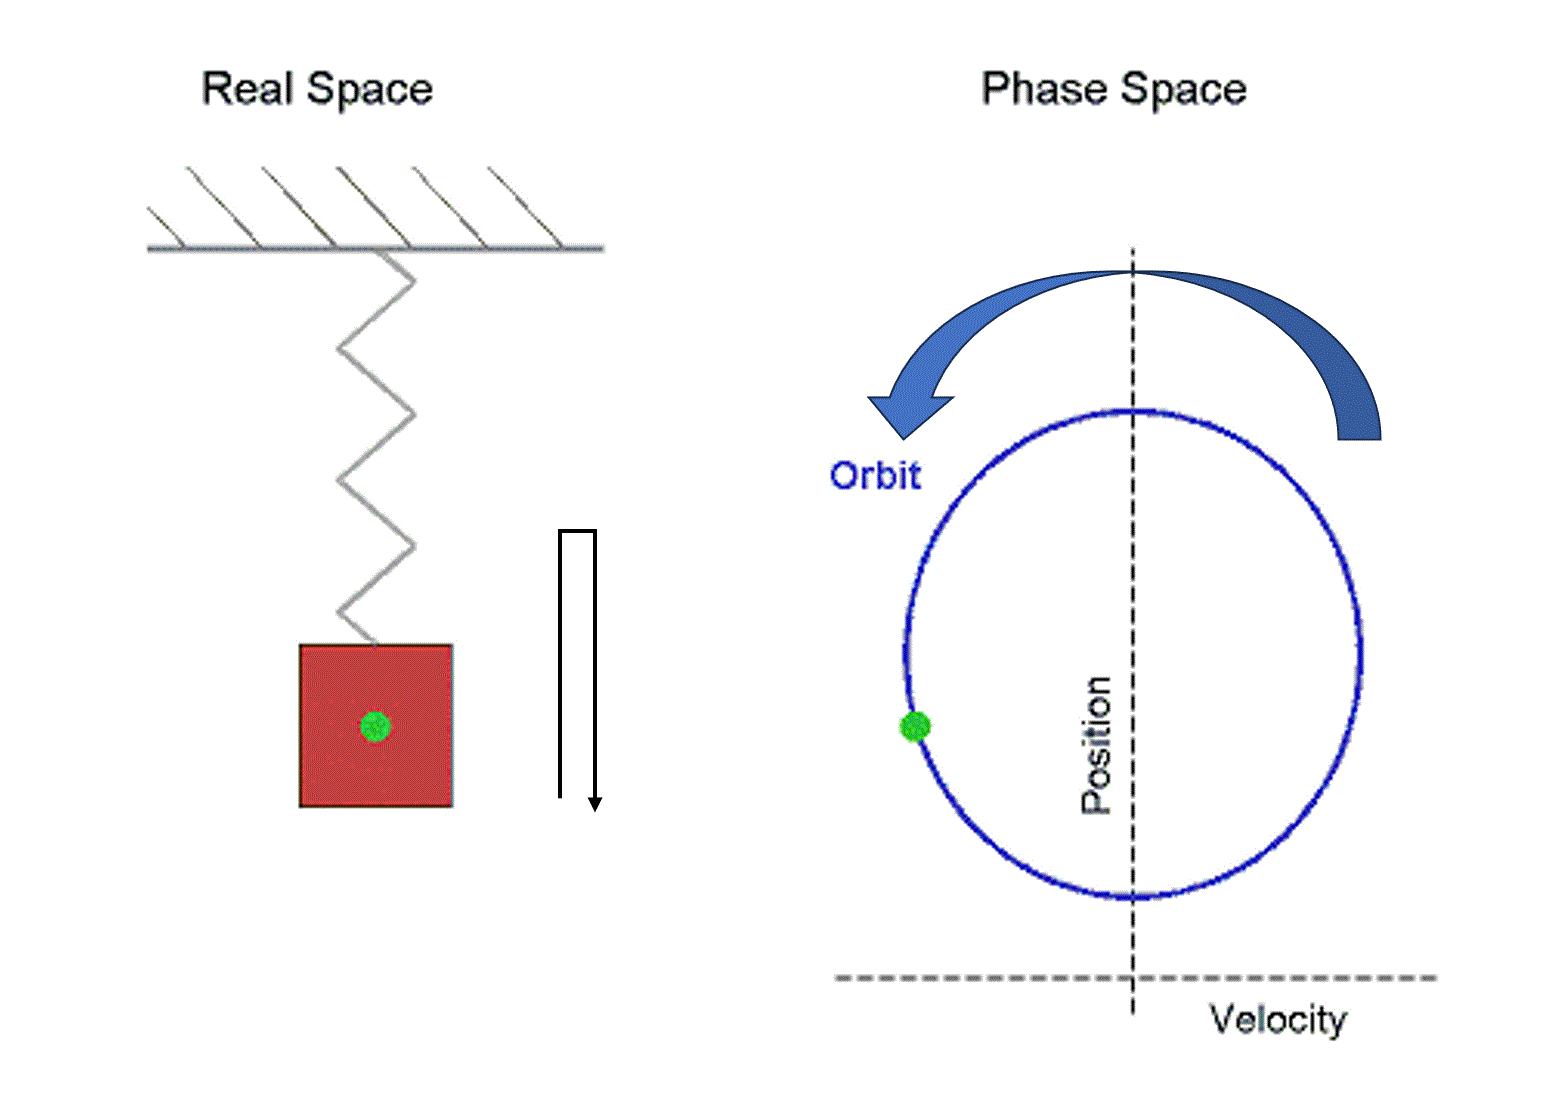
\includegraphics[height=180pt]{assets/Simple_Harmonic_Motion_Orbit.png}
    \captionof{figure}{Phase space of SHO}
\end{center}

\subsection*{(2) Using boundary conditions to find a solution
用边界条件计算简谐振子的解}\label{using-boundary-conditions-to-find-a-solution-ux7528ux8fb9ux754cux6761ux4ef6ux8ba1ux7b97ux7b80ux8c10ux632fux5b50ux7684ux89e3}

The basic function is \(\ddot{x} + \omega_0^2 x = 0\). Its general
solution is \[x = C_1 \cos \omega_0 t + C_2 \sin \omega_0 t.\]

To figure out the values of \(C_1\) and \(C_2\), we need boundary
conditions (边界条件) (for example, initial conditions), for example,
when \(t = 0\), \(x = x_0\) and
\(\displaystyle \frac{\mathrm{d}x}{\mathrm{d}t} = 0\).

In this scenario, when \(t = 0\):
\begin{itemize}
    \item \(x = C_1 = x_0\);
    \item \(\displaystyle \left. \frac{\mathrm{d}x}{\mathrm{d}t} \right|_{t = 0} = - \omega_0 C_1 \sin \omega_0 t + \omega_0 C_2 \cos \omega_0 t \Big|_{t = 0} = C_2 \omega_0 = 0\).
\end{itemize}

That is, \(C_1 = x_0\), and \(C_2 = 0\).

From \(C_2 = 0\), we can simplify \(x\) to \[x = x_0 \cos \omega_0 t.\]
Thus, we have
\[\frac{\mathrm{d}x}{\mathrm{d}t} = - \omega_0 x_0 \sin \omega_0 t\] and
\[\frac{\mathrm{d}^2 x}{\mathrm{d}t^2} = - \omega_0^2 x_0 \cos \omega_0 t = - \omega_0^2 x,\]
where \(\displaystyle \omega_0 = \sqrt{k \over m}.\)

\subsection*{(3) A general method to calculate the
equation of motion of a particle with known potential energy \(U(x)\)
and conserved energy \(E\)
解已知势能和守恒的总能量的质点的运动方程的一种通法}\label{a-general-method-to-calculate-the-equation-of-motion-of-a-particle-with-known-potential-energy-ux-and-conserved-energy-e-ux89e3ux5df2ux77e5ux52bfux80fdux548cux5b88ux6052ux7684ux603bux80fdux91cfux7684ux8d28ux70b9ux7684ux8fd0ux52a8ux65b9ux7a0bux7684ux4e00ux79cdux901aux6cd5}

The general method (under any given potential energy \(U(x)\)) is:
\[E = {1 \over 2} m \dot{x}^2 + U(x).\] From this, we can get
\[\frac{\mathrm{d}x}{\mathrm{d}t}  = \pm \sqrt{\frac{2}{m}[E - U(x)]}.\]
Integrate this, we can get
\[\int_{0}^{t} \mathrm{d}t = \int_{x_0}^{x} \pm \frac{\mathrm{d}x}{\sqrt{\dfrac{2}{m}[E - U(x)]}},\]
from which we can acquire the equation of motion.

\textbf{An example of using this method to solve the equation of motion
of SHO 用这种方法解出简谐振子方程的示例:}

In the particular case of SHO, we know the energy of the particle is
\[E = {1 \over 2} k x_0^2\] and the potential energy is
\[U(x) = {1 \over 2} k x^2.\]

Substitute \(E\) and \(U(x)\) in the equation above, and we have
\[\int_{0}^{t} \mathrm{d}t = \int_{x_0}^{x} \pm \frac{\mathrm{d}x}{\sqrt{\dfrac{2}{m}\left( \dfrac{1}{2} k x_0^2 - \dfrac{1}{2} k x^2 \right)}} = \int_{x_0}^{x} \pm \frac{\mathrm{d}x}{\omega_0 \sqrt{\left( x_0^2 - x^2 \right)}}\]
\[t = \pm {1 \over \omega_0} \arccos \left( {x \over x_0} \right)\]
\[\cos (\mp \omega_0 t) = {x \over x_0}\]
\[x = x_0 \cos \left( \mp \omega_0 t \right) = x_0 \cos \omega_0 t,\]
which is the equation of motion of the SHO.

\subsection*{(4) Series expansion of the equation of motion of the SHO
简谐振子运动方程的级数展开}\label{series-expansion-of-the-equation-of-motion-of-the-sho-ux7b80ux8c10ux632fux5b50ux8fd0ux52a8ux65b9ux7a0bux7684ux7ea7ux6570ux5c55ux5f00}

The basic form of the series expansion of \(x(t)\) is
\[x(t) = a_0 + a_1 t + a_2 t^2 + \cdots + a_n t^n + \cdots = a_0 + \sum_{i = 1}^{\infty} a_i x^i.\]

When \(t = 0\), \(x = x_0\), and therefore \(a_0 = x_0\).

Take the first derivative of \(x\), and we get
\[\frac{\mathrm{d}x}{\mathrm{d}t} = a_1 + 2a_2 t + \cdots + n a_n t^{n - 1} + \cdots.\]

When \(t = 0\), \(\displaystyle \frac{\mathrm{d}x}{\mathrm{d}t} = 0\),
and thus \(a_1 = 0\).

Take the second derivative of \(x\), and we get
\[\frac{\mathrm{d}^2x}{\mathrm{d}t^2} = 2a_2 + 6 a_3 t + 12 a_4 t^2 + \cdots + n(n - 1) a_n t^{n - 2} + \cdots.\]
Also, we know
\(\ddot{x} = - \omega_0^2 x = - \omega_0^2 \left( a_0 + a_1 t + a_2 t^2 + \cdots + a_n t^n + \cdots \right)\).
Therefore, we have \(6a_3 = - \omega_0^2 a_1\), and \(a_3 = a_1 = 0\).

Take more derivatives of \(x\), and in similar ways, we will know that
\[a_1 = a_3 = a_5 = \cdots = a_{2n + 1} = 0.\]

This conclusion can be verified by the series expansion of the cosine
function:
\[x = x_0 \cos \omega_0 t = x_0 \sum_{n = 0}^{\infty} \frac{(-1)^n x^{2n}}{(2n)!} = x_0 \left( 1 - \frac{x^2}{2} + \frac{x^4}{4!} - \frac{x^6}{6!} + \cdots \right).\]

\begin{quote}
作业:托尔斯泰《战争与和平》中的微积分体现在哪里?

比如人之将死,就是积分到了上限;期末考试积分的是你的所有的60个学时的努力。
\end{quote}

\emph{托尔斯泰的伟大可见一斑。}

\section{Features of an inertial coordinate system
惯性系的特征}\label{features-of-an-inertial-coordinate-system-ux60efux6027ux7cfbux7684ux7279ux5f81}

According to Landau, an inertial coordinate system has 3 aspects:

\begin{enumerate}
\def\labelenumi{\arabic{enumi}.}
\tightlist{} 
\item 
  Space:

  \begin{enumerate}
  \def\labelenumii{(\arabic{enumii})}
  \item
    Homogeneity (homogeneous) 空间同质性
    \[{\partial L \over \partial \boldsymbol{r}_\alpha} = \boldsymbol{0}\]
  \item
    Isotropy (isotropic) 空间各向同性
    \[\boldsymbol{v} \cdot \boldsymbol{v}, \boldsymbol{v}^4, \boldsymbol{v}^6, \cdots, \boldsymbol{v}^{2n}, \cdots \quad L(\boldsymbol{v} \cdot \boldsymbol{v}, t)\]
  \end{enumerate}
\item
  Time: Homogeneity 时间同质性
  \[L(\boldsymbol{v} \cdot \boldsymbol{v})\]
\item
  Simplicity 简单性
\end{enumerate}

\section{Galilean group
伽利略群}\label{galilean-group-ux4f3dux5229ux7565ux7fa4}

\emph{编者注:写这里的时候参考了\url{https://en.wikipedia.org/wiki/Galilean_transformation\#Galilean_transformations}.}

Here we use \((t, \boldsymbol{r})\) to express a general point in
spacetime (时空中任意一点).

The Galilean symmetries can be uniquely written as the composition of a
uniform motion of spacetime, a translation and a rotation:

\begin{enumerate}
\def\labelenumi{\arabic{enumi}.}
\item
  Uniform motion with velocity \(\boldsymbol{V}\)
  (速度为\(\boldsymbol{V}\)的匀速运动变换)

  \[g_1(t, \boldsymbol{r}) = (t, \boldsymbol{r} - \boldsymbol{V}t)\]

  This transformation has 3 dimensions.
\item
  Spatial and time translation (时间和空间平移变换)

  \[g_2(t, \boldsymbol{r}) = (t + \tau, \boldsymbol{r} + \boldsymbol{s})\]

  This transformation has 4 dimensions and is called an \textbf{affine
  transformation} (仿射变换).
\item
  Rotation (旋转变换)

  \[g_3(t, \boldsymbol{r}) = (t, \mathbf{R} \cdot \boldsymbol{r})\]

  This transformation has 3 dimensions.
\end{enumerate}

As a Lie group, the group of Galilean transformations has dimension
\(10 \ (3 + 4 + 3 = 10)\).

The Galilean Group is a highly generalized representation of Newtonian
mechanics. Newtonian mechanics is a group that holds under Galilean
transformations.
(伽利略群是对牛顿力学的高度概括。牛顿力学是伽利略变换不变的群。)

\chapter{2023/12/11}\label{20231211}

\emph{场论由 Faraday 于 1865
年提出,第一次运用是在笔记中出现了``field''这个词}

\emph{7岁学习微积分的陶哲轩大神:``直觉'' (intuition)}

\section{Two paradigms for classical mechanics
经典力学的两大范式}\label{two-paradigms-for-classical-mechanics-ux7ecfux5178ux529bux5b66ux7684ux4e24ux5927ux8303ux5f0f}

\textbf{Paradigm I:} Newton's 1st principle (第一性原理)

\textbf{Paradigm II:} Kepler's big data (大数据)

Kepler's big data established paradigms for all subjects.

\section{Data-driven (re)discovery of partial differential equations
数据驱动下对偏微分方程的(重)发现}\label{data-driven-rediscovery-of-partial-differential-equations-ux6570ux636eux9a71ux52a8ux4e0bux5bf9ux504fux5faeux5206ux65b9ux7a0bux7684ux91cdux53d1ux73b0}

From \emph{Science Advances}, \emph{Data-driven discovery of partial differential equations} (\url{https://doi.org/10.1126/sciadv.1602614}).

Examples:
\begin{itemize}
    \tightlist{}
    \item Navier-Stokes equations 纳维-斯托克斯方程 \[ {\partial \boldsymbol v \over \partial t} +(\boldsymbol v \cdot \nabla) \boldsymbol v = - {1 \over \rho} \nabla p + \mu \nabla^2 \boldsymbol v + \boldsymbol g\]
    \item Schrödinger Equation 薛定谔方程
    \[-{ \hbar^2 \over 2m } \nabla ^2 \psi + U \psi =i\hbar {\partial \psi \over \partial t}\]
    \item Korteweg--De Vries equation 科特韦赫-德弗里斯方程 / KdV方程
    \[\partial_t \phi + \partial^3_x \phi - 6 \phi \partial_x \phi =0\]
\end{itemize}

\section{Four paradigms
四种范式}\label{four-paradigms-ux56dbux79cdux8303ux5f0f}

For future reference, you can see the book
\emph{The Fourth Paradigm: Data-intensive Scientific Discovery} (2009) (\url{https://www.microsoft.com/en-us/research/uploads/prod/2009/10/Fourth_Paradigm.pdf}).

\begin{center}
    \begin{tabular}{|c|c|c|}
        \hline
        \textbf{Order} & \textbf{Contents} & \textbf{Base} \\
        \hline
        1st Paradigm & Experimental-based empirical science & Experiments \\
        \hline
        2nd Paradigm & Model-based theoretical science & Theoretical derivation \\
        \hline
        3rd Paradigm & Simulation-based numerical science & Computer simulations \\
        \hline
        4th Paradigm & Data-driven AI science & AI \\
        \hline
    \end{tabular}
    \captionof{table}{Four Paradigms in Science}
\end{center}

\begin{quote}
思考:第三点和第四点有什么区别?
\end{quote}

\section{AI for science
汤超院士:AI的三个层次}\label{ai-for-science-ux6c64ux8d85ux9662ux58ebaiux7684ux4e09ux4e2aux5c42ux6b21}

For the full text of Tang Chao's speech, please turn to the webpage \emph{2022科学智能峰会回顾|汤超院士:关于AI for Science的几层意思} (\url{http://www.aais.pku.edu.cn/news/shownews.php?id=1493}) for reference.

\emph{译者注:此部分先放中文在放英文,是因为原文为中文}

Tang Chao pointed out that there are 3 levels of AI application
nowadays:

\begin{enumerate}
\def\labelenumi{\arabic{enumi}.}
\item
  将深度学习技术用于各个学科中的科研、技术创新、成果转化等

  Applying deep learning technology to scientific research,
  technological innovation, and achievement transformation in various
  disciplines
\item
  利用AI来发现``new science''

  Using AI to discover ``new science''
\item
  AI背后的科学原理

  Science of AI
\end{enumerate}

Articles like \emph{Rediscovering orbital mechanics with machine learning} (\url{https://doi.org/10.1088/2632-2153/acfa63}) have pointed out that machine learning can be used to analyze big data and rediscover theorems in classical mechanics.

Researchers in the classical mechanics field should pay attention to
such advancements in AI and not stay away from them.

\section{Physical pendulum
物理摆}\label{physical-pendulum-ux7269ux7406ux6446}

\subsection*{(1) Random-shaped physical pendulum
一般的摆}\label{random-shaped-physical-pendulum-ux4e00ux822cux7684ux6446}

\begin{center}
    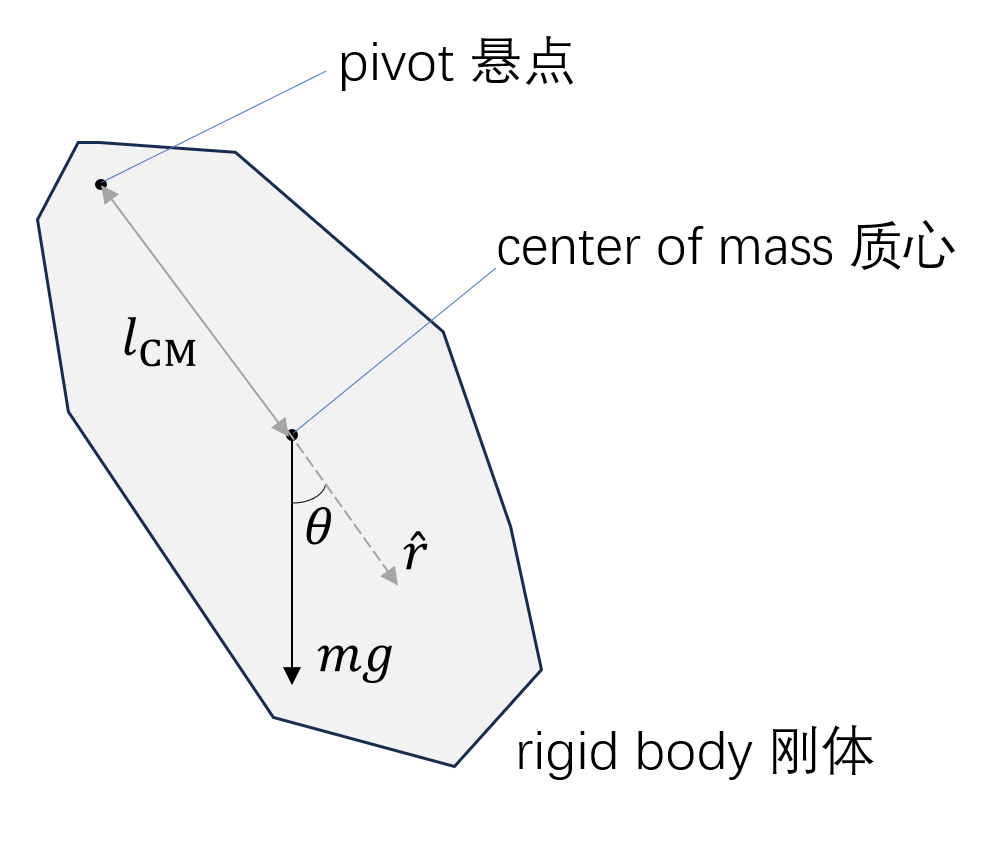
\includegraphics[height=150pt]{assets/Physical_pendulum.png}
    \captionof{figure}{Physical pendulum}
\end{center}

The gravity of the pendulum is
\[m\boldsymbol{g} = mg (\cos \theta \hat{\boldsymbol{r}} - \sin \theta \hat{\boldsymbol{\theta}}).\]

The torque is \begin{align*}
    \boldsymbol{M} & = \boldsymbol{r} \times m \boldsymbol{g} \\
    & = l_{\text{CM}} \hat{\boldsymbol{r}} \times mg (\cos \theta \hat{\boldsymbol{r}} - \sin \theta \hat{\boldsymbol{\theta}}) \\
    & = - l_{\text{CM}} mg \sin \theta \hat{\boldsymbol{k}}.
\end{align*}

According to the angular momentum theorem, we have
\[\boldsymbol{M} = - l_{\text{CM}} mg \sin \theta \hat{\boldsymbol{k}} = I \frac{\mathrm{d}^2 \theta}{\mathrm{d}t^2} \hat{\boldsymbol{k}}\]
\[I \ddot{\theta} + mgl_{\text{CM}} \sin \theta = 0.\]

When \(\theta \ll 1\),
\[\ddot{\theta} + \frac{mgl_{\text{CM}}}{I} \theta = 0.\]

\subsection*{(2) Torsional pendulum
扭摆}\label{torsional-pendulum-ux626dux6446}

\emph{编者吐槽:这图不会画}

Let the equilibrium position be \(\theta = 0\), and we know the torque
\[M = - k \theta.\]

Also, according to the angular momentum theorem,
\(M = I \ddot{\theta}\), and we have \[I \ddot{\theta} + k \theta = 0\]
\[\ddot{\theta} + \frac{k}{I} \theta = 0.\]

\section{Principle of virtual work/displacement
虚功/位移原理}\label{principle-of-virtual-workdisplacement-ux865aux529fux4f4dux79fbux539fux7406}

In a system with \(s\) degrees of freedom, we can write the position of
a particle \[\boldsymbol{r} = \boldsymbol{r}(q_1, q_2, \dots, q_s; t).\]

Take the time derivative of \(\boldsymbol{r}\) and we get
\[\boldsymbol{v} = \frac{\mathrm{d} \boldsymbol{r}}{\mathrm{d}t} = \frac{\partial \boldsymbol{r}}{\partial t} + \sum_{j = 1}^{s} \frac{\partial \boldsymbol{r}}{\partial q_j} \frac{\mathrm{d} q_j}{\mathrm{d}t}.\]

For a mechanical system at equilibrium, we know that
\[\delta W = \sum_{i = 1}^{n} \boldsymbol{F}_i \cdot \delta \boldsymbol{r}_i = \sum_{i = 1}^{n} \boldsymbol{F}_i \cdot \left( \sum_{j = 1}^{s} \frac{\partial \boldsymbol{r}_i}{\partial q_j} \delta q_j \right) = 0,\]
where \(n\) is the number of external forces applied on the system.

For each degree of freedom, there is a corresponding generalized force
\[Q_j = \sum_{i = 1}^{n} \boldsymbol{F}_i \cdot \frac{\partial \boldsymbol{r}_i}{\partial q_j}.\]

Also, we know that there are two types of forces: \textbf{active forces
(主动力)} and \textbf{constraint forces (约束力)}:
\[\boldsymbol{F}_i = \boldsymbol{F}_i^{\text{(a)}} + \boldsymbol{F}_i^{\text{(c)}},\]
and we can break \(\delta W\) into 2 parts:
\[\delta W = \sum_{i = 1}^{n} \sum_{j = 1}^{s} \boldsymbol{F}_i^{\text{(a)}} \cdot \frac{\partial \boldsymbol{r}_i}{\partial q_j} \delta q_j + \underline{\sum_{i = 1}^{n} \sum_{j = 1}^{s} \boldsymbol{F}_i^{\text{(c)}} \cdot \frac{\partial \boldsymbol{r}_i}{\partial q_j} \delta q_j}.\]

The underlined part (the work of the constraint forces) is usually
\(0\), and we only need to calculate the first part. That is,
\[\sum_{i = 1}^{n} \sum_{j = 1}^{n} \boldsymbol{F}_i^{\text{(a)}} \cdot \frac{\partial \boldsymbol{r}_i}{\partial q_j} \delta q_j = 0.\]

\chapter{2023/12/13}\label{20231213}

\emph{Elon Musk (1971\textasciitilde{} ): First-principle thinking
第一性原理思考:从某一体系的物理本质思考问题}

\emph{越南在明朝之前是中国领土。之后官员搜刮民脂民膏导致当地造反,官员将此事瞒了下来。这是不符合第一性原理的!}

\section{D'Alembert's principle (1743)
达朗贝尔原理}\label{dalmberts-principle-1743-ux8fbeux6717ux8d1dux5c14ux539fux7406}

\subsection*{(1) Contents 内容}\label{contents-ux5185ux5bb9-2}

This principle is hailed as the first principle of theoretical mechanics
(理论力学的第一性原理).

In the system, there are \(s\) particles, and for particle \(i\), its
position vector is
\[\boldsymbol{r}_i = \boldsymbol{r}_i (q_1, q_2, \dots, q_s; t).\]

Particle \(i\) can make real displacements (实位移):
\[\mathrm{d} \boldsymbol{r}_i = \frac{\partial \boldsymbol{r}_i}{\partial t} \mathrm{d}t + \sum_{j = 1}^{s} \frac{\partial \boldsymbol{r}_i}{\partial q_j} \mathrm{d}q_j\]
and we can know its virtual displacement (虚位移):
\[\delta \boldsymbol{r}_i = \sum_{j = 1}^{s} \frac{\partial \boldsymbol{r}_i}{\partial q_j} \delta q_j.\]

From real displacement \(\mathrm{d} \boldsymbol{r}_i\), we can know the
real velocity (实速度) of particle \(i\):
\[\boldsymbol{v}_i = \frac{\mathrm{d} \boldsymbol{r}_i}{\mathrm{d}t} = \frac{\partial \boldsymbol{r}_i}{\partial t} + \sum_{j = 1}^{s} \frac{\partial \boldsymbol{r}_i}{\partial q_j} \frac{\mathrm{d}q_j}{\mathrm{d}t} = \frac{\partial \boldsymbol{r}_i}{\partial t} + \sum_{j = 1}^{s} \frac{\partial \boldsymbol{r}_i}{\partial q_j} \dot{q}_j.\]

From this, we can know that
\[\frac{\partial \boldsymbol{v}_i}{\partial \dot{q}_j} = \sum_{j = 1}^{s} \frac{\partial \boldsymbol{r}_i}{\partial q_j}.\]

Through this, we have reduced a dynamic problem to a static one
(化动为静).

According to the principle of virtual work, we can know
\[\sum_{i = 1}^{n} \boldsymbol{F}_i \cdot \delta \boldsymbol{r}_i = \boldsymbol{0}.\]
According to the Newton's 2nd law of motion, we know that
\[\boldsymbol{F}_i = \frac{\mathrm{d} \boldsymbol{p}_i}{\mathrm{d}t}.\]
From the two equations above, we know that
\[\sum_{i = 1}^{n} \left( \boldsymbol{F}_i - \frac{\mathrm{d} \boldsymbol{p}_i}{\mathrm{d}t} \right) \cdot \delta \boldsymbol{r}_i = 0.\]

This is the \textbf{D'Alembert's principle (达朗贝尔原理)}. It can also
be written in this form:
\[\sum_{i = 1}^{n} \left( \boldsymbol{F}_i - m_i \ddot{\boldsymbol{r}}_i \right) \cdot \delta \boldsymbol{r}_i = 0.\]

\subsection*{(2) Using D'Alembert's principle to derive the
Euler-Lagrange equation
用达朗贝尔原理推导欧拉-拉格朗日方程}\label{using-dalmberts-principle-to-derive-the-euler-lagrange-equation-ux7528ux8fbeux6717ux8d1dux5c14ux539fux7406ux63a8ux5bfcux6b27ux62c9-ux62c9ux683cux6717ux65e5ux65b9ux7a0b}

Generalized force \(Q_j\) is defined as follows:
\[\sum_{i = 1}^{n} \boldsymbol{F}_i \cdot \delta \boldsymbol{r}_i = \sum_{i = 1}^{n} \boldsymbol{F}_i \cdot \left( \sum_{j = 1}^{s} \frac{\partial \boldsymbol{r}_i}{\partial q_j} \delta q_j \right) = \sum_{j = 1}^{s} Q_j \delta q_j = 0. \quad(1)\]

Also, we have \begin{align*}
    \sum_{i = 1}^{n} \boldsymbol{F}_i \cdot \delta \boldsymbol{r}_i & = \sum_{i = 1}^{n} \frac{\mathrm{d} \boldsymbol{p}_i}{\mathrm{d}t} \cdot \left( \sum_{j = 1}^{s} \frac{\partial \boldsymbol{r}_i}{\partial q_j} \delta q_j \right) = \sum_{i = 1}^{n} \sum_{j = 1}^{s}  m_i \frac{\mathrm{d}^2 \boldsymbol{r}}{\mathrm{d}t^2} \cdot \frac{\partial \boldsymbol{r}_i}{\partial q_j} \delta q_j \\
    & = \sum_{i = 1}^{n} \sum_{j = 1}^{s}  m_i \frac{\mathrm{d}}{\mathrm{d}t} \left( \frac{\mathrm{d} \boldsymbol{r}_i}{\mathrm{d}t} \right) \cdot \frac{\partial \boldsymbol{r}_i}{\partial q_j} \delta q_j \\
\end{align*}
\begin{align*}    
    & = \sum_{i = 1}^{n} \sum_{j = 1}^{s}  \left[ \frac{\mathrm{d}}{\mathrm{d}t} \left( m_i \frac{\mathrm{d} \boldsymbol{r}_i}{\mathrm{d}t} \cdot \frac{\partial \boldsymbol{r}_i}{\partial q_j} \right) - m_i \frac{\mathrm{d} \boldsymbol{r}_i}{\mathrm{d}t} \cdot \frac{\mathrm{d}}{\mathrm{d}t} \left( \frac{\partial \boldsymbol{r}_i}{\partial q_j} \right) \right] \delta q_j \\
    & = \sum_{i = 1}^{n} \sum_{j = 1}^{s}  \left[ \frac{\mathrm{d}}{\mathrm{d}t} \left( m_i \boldsymbol{v}_i \cdot \frac{\partial \boldsymbol{v}_i}{\partial \dot{q}_j} \right) - m_i \boldsymbol{v}_i \cdot \frac{\partial}{\partial q_j} \left( \frac{\mathrm{d} \boldsymbol{r}_i}{\mathrm{d}t} \right) \right] \delta q_j \\
    & = \sum_{i = 1}^{n} \sum_{j = 1}^{s}  \left[ \frac{\mathrm{d}}{\mathrm{d}t} \frac{\partial}{\partial \dot{q}_j} \left( {1 \over 2} m_i  {v}_i^2 \right) - \frac{\partial}{\partial q_j} \left( {1 \over 2} m_i  {v}_i^2 \right) \right] \delta q_j \\
    & = \sum_{i = 1}^{n} \sum_{j = 1}^{s}  \left( \frac{\mathrm{d}}{\mathrm{d}t} \frac{\partial T}{\partial \dot{q}_j} - \frac{\partial T}{\partial q_j} \right) \delta q_j \\
    & = 0. \quad(2)
\end{align*}

\emph{编者:精髓就是:凑,就硬凑}

\((1) - (2)\), and we get:
\[\sum_{j = 1}^{s} \left( Q_j - \frac{\mathrm{d}}{\mathrm{d}t} \frac{\partial T}{\partial \dot{q}_j} + \frac{\partial T}{\partial q_j} \right) \delta q_j = 0.\]

Because \(\delta q_j\) ia arbitrary (随意选取的), we need
\[ Q_j - \frac{\mathrm{d}}{\mathrm{d}t} \frac{\partial T}{\partial \dot{q}_j} + \frac{\partial T}{\partial q_j} = 0, \quad(*)\]
where \(Q_j\) is conservative, generalized force (保守的广义力).

Correspondingly, we have a pair of work conjugates (功的共轭):
\[\text{Work conjugate}
\left\{
\begin{array}{ll}
    \boldsymbol{F} & \mathrm{d} \boldsymbol{r} \\
    Q & \delta q
\end{array}
\right.\]

Also we know that \[\frac{\partial V}{\partial \dot{q}_j} = 0\] and
\[Q_j = - \frac{\partial V}{\partial q_j}.\] Substitute these two
equations in \((*)\), and we get
\[- \frac{\partial V}{\partial q_j} - \frac{\mathrm{d}}{\mathrm{d}t} \frac{\partial (T - V)}{\partial \dot{q}_j} + \frac{\partial T}{\partial q_j} = 0\]
\[\frac{\partial (T - V)}{\partial q_j} - \frac{\mathrm{d}}{\mathrm{d}t} \frac{\partial (T - V)}{\partial \dot{q}_j} = 0\]
\[\frac{\partial L}{\partial q_j} - \frac{\mathrm{d}}{\mathrm{d}t} \frac{\partial L}{\partial \dot{q}_j} = 0,\]
where \(L\) is the Lagrangian. This is the Euler-Lagrange equation.

\section{Vibration of a string
弦的振动}\label{vibration-of-a-string-ux5f26ux7684ux632fux52a8}

\emph{编者按:此部分涉及到欧拉-拉格朗日方程的多变量推广。具体的推导可以参考这篇文章:【变分计算2】多变量系统下的变分方程
(\url{https://zhuanlan.zhihu.com/p/357217956})。}

Suppose there is an infinitesimal movement \(u(x, t)\) on a piece of
string whose length is \(L\).

The kinetic energy (动能) of the string is
\[E_k = \int_{0}^{L} {1 \over 2} \mu \left( \frac{\partial u}{\partial t} \right)^2 \mathrm{d}x,\]
where \(\displaystyle \mu = \frac{m}{L}\) is the linear mass density
(质量线密度).

For an infinitesimal length on the string from \(x\) to
\(x + \mathrm{d}x\), when vibrating, its length becomes
\[\mathrm{d}l' = \sqrt{1 + \left( \frac{\partial u}{\partial x} \right)^2} \mathrm{d}x,\]
and the change in length is
\[\mathrm{d}l' - \mathrm{d}x = \left( \sqrt{1 + \left( \frac{\partial u}{\partial x} \right)^2} - 1 \right) \mathrm{d}x \approx \left[ 1 + \frac{1}{2} \left( \frac{\partial u}{\partial x} \right)^2 - 1 \right] = \frac{1}{2} \left( \frac{\partial u}{\partial x} \right)^2 \mathrm{d}x.\]

The potential energy is
\[U = - W = \int T (\mathrm{d}l' - \mathrm{d}x) = \int_{0}^{L} \frac{1}{2} T \left( \frac{\partial u}{\partial x} \right)^2 \mathrm{d}x.\]

The Lagrangian is
\[L = E_k - U = \int_{0}^{L} \frac{1}{2} \left[ \mu \left( \frac{\partial u}{\partial t} \right)^2 - T \left( \frac{\partial u}{\partial x} \right)^2 \right] \mathrm{d}x = \int_{0}^{L} \mathcal{L} \mathrm{d}x,\]
where \(\mathcal{L}\) is the Lagrangian density (拉格朗日量密度).

\(\mathcal{L}\) can be written in this form:
\[\mathcal{L} = \mathcal{L} \left( u, \frac{\partial u}{\partial x}, \frac{\partial u}{\partial t}; x, t \right).\]

Because the Lagrangian is a functional (泛函) of \(u(x, t)\), we can
expand the Euler-Lagrange equation to
\[\frac{\partial}{\partial t} \frac{\partial \mathcal{L}}{\partial (\partial u / \partial t)} + \frac{\partial}{\partial x} \frac{\partial \mathcal{L}}{\partial (\partial u / \partial x)} - \frac{\partial \mathcal{L}}{\partial u} = 0. \quad(*)\]

Here,
\(\displaystyle \mathcal{L} = \frac{1}{2} \left[ \mu \left( \frac{\partial u}{\partial t} \right)^2 - T \left( \frac{\partial u}{\partial x} \right)^2 \right]\)
does not depend on \(u\), and thus \(u\) is a cyclic coordinate
(循环坐标).

Substitute \(\mathcal{L}\) into \((*)\), and we get
\[\mu \frac{\partial^2 u}{\partial t^2} - T \frac{\partial^2 u}{\partial x^2} = 0,\]
\[\left( \frac{1}{c^2} \frac{\partial^2}{\partial t^2} - \frac{\partial^2}{\partial x^2} \right) u = \Box u = 0.\]
Here \(\Box\) is called the \textbf{d'Alembert or quabla operator
(达朗贝尔算符)}:
\[\Box = \frac{1}{c^2} \frac{\partial^2}{\partial t^2}- \nabla^2.\]

\section{Vibration of a membrane
膜的振动}\label{vibration-of-a-membrane-ux819cux7684ux632fux52a8}

Suppose the membrane has an area density (质量面密度) of
\(\varLambda = \rho h\) (where \(h\) is the thickness of the membrane),
and its surface tension coefficient (表面张力系数, surface tension per
unit length) is \(\sigma\).

Similar to the vibration of strings, we have the Lagrangian density
\[\mathcal{L} = \frac{1}{2} \left\{ \varLambda \left( \frac{\partial u}{\partial t} \right)^2 - T \left[ \left( \frac{\partial u}{\partial x} \right)^2 + \left( \frac{\partial u}{\partial y} \right)^2 \right] \right\}\]
and equation of movement
\[\frac{\partial}{\partial t} \frac{\partial \mathcal{L}}{\partial (\partial u / \partial t)} + \frac{\partial}{\partial x} \frac{\partial \mathcal{L}}{\partial (\partial u / \partial x)} + \frac{\partial}{\partial y} \frac{\partial \mathcal{L}}{\partial (\partial u / \partial y)} - \frac{\partial \mathcal{L}}{\partial u} = 0\]
and solution
\[\left( \frac{1}{c^2} \frac{\partial^2}{\partial t^2} - \frac{\partial^2}{\partial x^2} - \frac{\partial^2}{\partial y^2} \right) u = \Box u = 0.\]

\begin{quote}
作业:Arnold《经典力学的数学方法》书中,为什么说所有生物跳的高度是同一量级?
\end{quote}

\chapter{2023/12/18}\label{20231218}

\section{Vibration of a one-dimensional semi-infinite rod
一维半无限长杆的振动}\label{vibration-of-a-one-dimensional-semi-infinite-rod-ux4e00ux7ef4ux534aux65e0ux9650ux957fux6746ux7684ux632fux52a8}

\begin{center}
    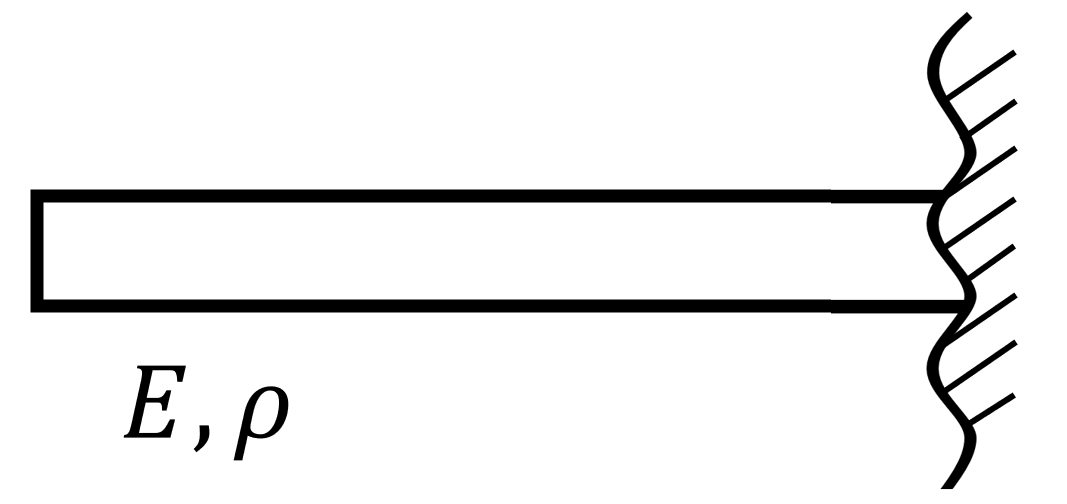
\includegraphics[height=40pt]{assets/One-dimensional_semi-infinite_rod.png}
    \captionof{figure}{One-dimensional semi-infinite rod}
\end{center}

As shown in Fig 27.1, we assume that the rod has density \(\rho\) and Young's modulus
(杨氏模量) \(E\).

\subsection*{(1) Dimensional analysis
量纲分析}\label{dimensional-analysis-ux91cfux7eb2ux5206ux6790}

The dimension of density and Young's modulus are
\[[E] = \frac{[F]}{[A]} = \frac{\mathrm{MLT^{-2}}}{\mathrm{L^2}} = \mathrm{ML^{-1}T^{-2}}\]
and \[[\rho] = \mathrm{ML^{-3}}.\]
\[\left[ \frac{E}{\rho} \right] = \mathrm{L^2 T^{-2}} = [c^2],\] and
thus we know \[c \sim \sqrt{\frac{E}{\rho}}.\]

\subsection*{(2) Lagrangian mechanics
拉格朗日力学}\label{lagrangian-mechanics-ux62c9ux683cux6717ux65e5ux529bux5b66}

The kinetic energy, written as the integral of a segment of the rod from
\(x\) to \(x + \mathrm{d}x\) is
\[T = \int_{0}^{+\infty} \frac{1}{2} \rho A \mathrm{d}x \left( \frac{\partial u}{\partial t} \right)^2,\]
and the potential energy is
\[U = \int_{0}^{+\infty} \frac{1}{2} EA \left( \frac{\partial u}{\partial x} \right)^2 \mathrm{d}x.\]

Write \(L = T - U\) as
\[L = \int_{0}^{+\infty} \mathcal{L} \mathrm{d}x,\] and we have
\[\mathcal{L} = \frac{1}{2} \left[ \rho \left( \frac{\partial u}{\partial t} \right)^2 - E \left( \frac{\partial u}{\partial x} \right)^2 \right]A.\]

According to the expanded Euler-Lagrangian equations, putting \(x\) and
\(t\) in the same position, we know
\[\frac{\partial}{\partial t} \frac{\partial \mathcal{L}}{\partial (\partial u / \partial t)} + \frac{\partial}{\partial x} \frac{\partial \mathcal{L}}{\partial (\partial u / \partial x)} - \frac{\partial \mathcal{L}}{\partial u} = 0,\]
and we get
\[\left( \frac{1}{c^2} \frac{\partial^2}{\partial t^2} - \frac{\partial^2}{\partial x^2} \right) u = \Box u = 0,\]
where \[c = \sqrt{\frac{E}{\rho}}.\]

\section[Deriving Hamilton's canonical equations 推导哈密顿正则方程]{Derivation of Hamilton's canonical equations
哈密顿正则方程的推导}\label{derivation-of-hamiltons-canonical-equations-ux54c8ux5bc6ux987fux6b63ux5219ux65b9ux7a0bux7684ux63a8ux5bfc}

\subsection*{(1) Conjugate variable pairs
共轭变量对}\label{conjugate-variable-pairs-ux5171ux8f6dux53d8ux91cfux5bf9}

\begin{itemize}
\tightlist{}
\item
  Thermodynamics

  In thermodynamics, we have conjugate pairs
  \(\left\{ \begin{array}{l}T \\ S \end{array} \right.\),
  \(\left\{ \begin{array}{l} p \\ V \end{array} \right.\) and
  \(\left\{ \begin{array}{l} \mu \\ N \end{array} \right.\), and
  correspondingly we have the \textbf{fundamental thermodynamic relation
  (热力学基本方程)}:
  \[\mathrm{d}U = T \mathrm{d}S - p \mathrm{d}V + \sum_i \mu_i \mathrm{d}N_i.\]

  \emph{编者注:课上赵老师写的是
  \(\mathrm{d}F = \mathrm{d}U - T \mathrm{d}S + p \mathrm{d}V + \mu \mathrm{d}n\),查询热力学教材、维基百科等资料发现疑似有误。}
\item
  Work conjugate

  In analytical mechanics, we have one famous conjugate pair of force
  and generalized force \[\left\{
        \begin{array}{ll}
            \boldsymbol{F} & \mathrm{d} \boldsymbol{r} \\
            Q & \delta q
        \end{array}
    \right.\] and they have the relation
  \[\sum_{i = 1}^{n} \boldsymbol{F}_i \cdot \delta \boldsymbol{r}_i = \sum_{i = 1}^{n} \boldsymbol{F}_i \cdot \left( \sum_{j = 1}^{s} \frac{\partial \boldsymbol{r}_i}{\partial q_j} \delta q_j \right) = \sum_{j = 1}^{s} \left( \sum_{i = 1}^{n} \boldsymbol{F}_i \cdot \frac{\partial \boldsymbol{r}_i}{\partial q_j} \right) \delta q_j = \sum_{j = 1}^{s} Q_j \delta q_j.\]
\item
  Generalized coordinates conjugate

  \[\left\{
    \begin{array}{ll}
        \displaystyle Q_j = \frac{\partial L}{\partial q_j} \quad \quad & \delta q_j  \\[1.5ex]
        \displaystyle p_j = \frac{\partial L}{\partial \dot{q_j}} & \dot{q_j}
    \end{array}
    \right.\]
\end{itemize}

\subsection*{(2) Advantages and drawbacks of Lagrangian mechanics
拉格朗日力学的优势和缺陷}\label{advantages-and-drawbacks-of-lagrangian-mechanics-ux62c9ux683cux6717ux65e5ux529bux5b66ux7684ux4f18ux52bfux548cux7f3aux9677}

\begin{itemize}
\tightlist{}
\item
  Advantage:

  Newtonian mechanics is a kind of mechanics illustrated graphically,
  while Lagrangian mechanics utilizes the energy method (使用能量方法)
  and stands at a higher level.
\item
  Drawbacks:

  \begin{enumerate}
  \def\labelenumi{\arabic{enumi}.}
  \tightlist{}
  \item
    From
    \(\displaystyle {\partial L \over \partial{q}_j} = {\mathrm{d} \over \mathrm{d}t} {\partial L \over \partial \dot{q}_j}\),
    we can see that \({q}_j\) and \(\dot{q}_j\) are not equal.
  \item
    The dimension system is complicated. For example, if \(q_1\) has a
    length dimension, then \(q_1 \dot{q}_1\) has a dimension of
    \(\mathrm{L^2T^{-1}}\); if \(q_2\) has an angle dimension, then
    \(q_1 \dot{q}_1\) has a dimension of \(\mathrm{T^{-1}}\). These two
    don't match.
  \end{enumerate}

  Hamiltonian mechanics uses \(q_j\) and \(p_j\) as its basic
  coordinates, and we know that \(q_j p_j\) has the dimension of action:
  \[[q_j p_j] = [E] \cdot [t].\]

  \emph{所以说,哈密顿力学比拉格朗日力学更美,是经典力学美的高峰。}
\end{itemize}

\subsection*{(3) Mathematical form of Legendre transformation
勒让德变换的数学形式}\label{mathematical-form-of-legendre-transformation-ux52d2ux8ba9ux5fb7ux53d8ux6362ux7684ux6570ux5b66ux5f62ux5f0f}

Suppose we have a function \(f = f(x, y)\).

Take the total differential of \(f\), and we acquire
\[\mathrm{d}f = \frac{\partial f}{\partial x} \mathrm{d}x + \frac{\partial f}{\partial y} \mathrm{d}y.\]

Here, we let \(\displaystyle u = \frac{\partial f}{\partial x}\) and
\(\displaystyle v = \frac{\partial f}{\partial y}\). Introduce a new
function \(g = ux - f\), and the differential of \(g\) is
\[\mathrm{d}g = u \mathrm{d}x + x \mathrm{d}u - \mathrm{d}f = x \mathrm{d}u - v \mathrm{d}y.\]

\subsection*{(4) Using Legendre transformation to derive the
Hamilton's canonical equations
用勒让德变换推导哈密顿正则方程}\label{using-legendre-transformation-to-derive-the-hamiltons-canonical-equations-ux7528ux52d2ux8ba9ux5fb7ux53d8ux6362ux63a8ux5bfcux54c8ux5bc6ux987fux6b63ux5219ux65b9ux7a0b}

In the derivation above, let \(f\) be the Lagrangian \(L\), \(g\) be the
Hamiltonian \(H\), \(x\) be the generalized velocity \(\dot{q}\) and
\(y\) be the generalized coordinate \(q\). Substitute this in, and we
get \[H = \dot{p} \dot{q} - L.\]

According to this, we can present the \textbf{Legendre transformation
(勒让德变换)} in analytical mechanics. In a system with \(n\) particles
and \(s\) generalized coordinates,
\[H = \sum_{j = 1}^{s} p_j \dot{q}_j - L.\]

Take the differential of both sides ,and we get
\[\mathrm{d}H = \sum_{j = 1}^{s} \left( p_j \mathrm{d} \dot{q}_j + \dot{q}_j \mathrm{d} p_j \right) - \mathrm{d}L. \quad(1)\]

Take the total derivative of \(L = L(q_j, \dot{q}_j, t)\), and we know
that \begin{align*}
    \mathrm{d}L & = \frac{\partial L}{\partial t} \mathrm{d}t + \sum_{j = 1}^{s} \left( \frac{\partial L}{\partial q_j} \mathrm{d}q_j + \frac{\partial L}{\partial \dot{q}_j} \mathrm{d} \dot{q}_j \right) \\
    & = \frac{\partial L}{\partial t} \mathrm{d}t + \sum_{j = 1}^{s} \left( \dot{p}_j \mathrm{d}q_j + {p}_j \mathrm{d} \dot{q}_j \right). \quad(2)
\end{align*}

Substitute \((2)\) into \((1)\), and we get
\[\mathrm{d}H = \sum_{j = 1}^{s} \dot{q}_j \mathrm{d} p_j - \sum_{j = 1}^{s} \dot{p}_j \mathrm{d}q_j - \frac{\partial L}{\partial t} \mathrm{d}t. \quad(3)\]

Also, because \(H = H(q_j, p_j, t)\), take the full derivative of \(H\)
and we get
\[\mathrm{d}H = \frac{\partial H}{\partial t} \mathrm{d}t + \sum_{j = 1}^{s} \left( \frac{\partial H}{\partial q_j} \mathrm{d}q_j + \frac{\partial H}{\partial p_j} \mathrm{d} p_j \right). \quad(4)\]

Compare equations \((3)\) and \((4)\) to observe that \[\left\{
    \begin{aligned}
        \frac{\partial H}{\partial q_j} &= -\dot{p}_j, \\
        \frac{\partial H}{\partial p_j} &= \dot{q}_j,
    \end{aligned}
\right.\] which are the \textbf{Hamiltonian Canonical equations
(哈密顿正则方程)}.

\subsection*{(5) SHO example
以简谐振子为例}\label{sho-example-ux4ee5ux7b80ux8c10ux632fux5b50ux4e3aux4f8b}

Use the displacement from the equilibrium point \(x\) as the generalized
coordinate, and the Hamiltonian and Lagrangian of the SHO are
\[H = \frac{p^2}{2m} + U(x)\] and
\[L = \frac{1}{2} m \dot{x}^2 - \frac{1}{2} kx^2.\]

Using Legendre transformation, we acquire
\[H = p \dot{x} - L = m \dot{x}^2 - \left( \frac{1}{2} m \dot{x}^2 - \frac{1}{2} kx^2 \right) = \frac{1}{2} m \dot{x}^2 + \frac{1}{2} kx^2 = \frac{p^2}{2m} + \frac{1}{2} kx^2.\]

Substitute \(H\) into the Hamiltonian Canonical equations, and we
acquire \[- \dot{p} = \frac{\partial H}{\partial x} = kx\] and
\[\dot{x} = \frac{\partial H}{\partial p} = \frac{p}{m}.\]

Take the time derivative of \(\displaystyle \dot{x} = \frac{p}{m}\),
substitute the result into \(-\dot{p} = kx\), and we get
\[m \ddot{x} = - kx,\] \[\ddot{x} + \frac{k}{m} x = 0,\]
\[\ddot{x} + \omega^2_0 x = 0.\]

Also, we can put the SHO into phase space (相空间) \((x, p)\) and we can
get an ellipse (椭圆). Every dot in the phase space represents a
possible state of the SHO. All the dots in the phase space, i.e.~all
possible states of the SHO, form the ellipse known as the \textbf{phase
trajectory (相轨道)}. The direction of the phase flow (相流) is
clockwise (顺时针).

\begin{center}
    \begin{tikzpicture}[scale=1.5]
        \draw[->] (-2, 0) -- (2,0) node[below] {$x$};
        \draw[->] (0, -2) -- (0,2) node[left] {$p$};
          
        \node at (1.5, 0) [above right] {$\sqrt{2E / k}$};
        \node at (0, 1) [above left] {$\sqrt{2mE}$};
        
        \draw[->] (1.299, -0.5) arc (330:-30:1.5 and 1);
        
        \node at (1.7, 1.3) {Phase trajectory};
        \node at (1.3, -0.5)[below right] {Direction of phase flow};
    \end{tikzpicture}
    \captionof{figure}{Phase space of SHO}
\end{center}

Suppose the initial phase (初相位) of the SHO is \(\varphi_0\), and we know
\[x = \sqrt{\frac{2E}{k}} \cos \left( \sqrt{\frac{k}{m}} t + \varphi_0 \right)\]
and
\[p = - \sqrt{2mE} \sin \left( \sqrt{\frac{k}{m}} t + \varphi_0 \right).\]

\subsection*{(6) The conservation of the Hamiltonian
哈密顿量的守恒}\label{the-conservation-of-the-hamiltonian-ux54c8ux5bc6ux987fux91cfux7684ux5b88ux6052}

When we look again at equations \((3)\) and \((4)\), we can see that
\[- \frac{\partial L}{\partial t} = \frac{\partial H}{\partial t}.\]

When Lagrangian \(L\) does not depend on \(t\),
\(\displaystyle \frac{\partial L}{\partial t} = 0\), and thus
\(\displaystyle \frac{\partial H}{\partial t} = 0\).

Using \((4)\), we can get \begin{align*}
    \frac{\mathrm{d}H}{\mathrm{d}t} & = \frac{\partial H}{\partial t} + \sum_{j = 1}^{s} \left( \frac{\partial H}{\partial q_j} \frac{\mathrm{d}q_j}{\mathrm{d}t} + \frac{\partial H}{\partial p_j} \frac{\mathrm{d} p_j}{\mathrm{d}t} \right) \\
    & = \frac{\partial H}{\partial t} + \sum_{j = 1}^{s} \left( - \dot{p}_j \dot{q}_j + \dot{q}_j \dot{p}_j \right) \\
    & = 0,
\end{align*} and this suggests that the Hamiltonian \(H\) is
conserved.

\begin{quote}
作业:哈密顿信奉的科学哲学是什么?
\end{quote}

\chapter{2023/12/20}\label{20231220}

\emph{做出任何选择都要进行风险评估。可能的风险包括但不限于政策风险、技术风险、资金风险等。}

\section{Earthquakes 地震}\label{earthquakes-ux5730ux9707}

\emph{编者按:据中国地震台网消息,2023年12月18日23时59分,甘肃省临夏回族自治州积石山保安族东乡族撒拉族自治县发生6.2级地震。习近平总书记对此作出重要指示:全力开展搜救,妥善安置受灾群众。}

In 1997, \emph{Science} published \emph{Earthquakes
Cannot Be Predicted (\url{https://doi.org/10.1126/science.275.5306.1616})}, and till this day, no one has raised any
objections against the viewpoint.

\emph{地震局的人,坐在宽敞的办公室,吃饭睡觉写文章,写出的文章也只能引用美国研究的观点,但也不能成功预报出地震。}

The happening of earthquakes is a chaotic system (混沌系统), and thus
difficult to predict. The abstract of the article above states:

\begin{quote}
Can the time, location, and magnitude of future earthquakes be predicted
reliably and accurately? In their Perspective, Geller et al.'s answer is
``no.'' \textbf{Citing recent results from the physics of nonlinear
systems ``chaos theory,'' they argue that any small earthquake has some
chance of cascading into a large event. According to research cited by
the authors, whether or not this happens depends on unmeasurably fine
details of conditions in Earth's interior.} Earthquakes are therefore
inherently unpredictable. Geller et al.~suggest that controversy over
prediction lingers because prediction claims are not stated as
objectively testable scientific hypotheses, and due to overly optimistic
reports in the mass media.
\end{quote}

In 2018, \emph{Nature} published \emph{Deep learning of aftershock patterns following large earthquakes} (\url{https://doi.org/10.1038/s41586-018-0438-y}), marking a new era of earthquake studies using AI technology.

\emph{聪明的人已经在做数据库来让AI学习了!}

\section{Phase space 相空间}\label{phase-space-ux76f8ux7a7aux95f4}

\[H = \sum_{j = 1}^{s} \frac{\partial L}{\partial \dot{q}_j} \dot{q}_j - L = 2T - (T - V) = T + V.\]

\emph{编者按:不知道这个式子跟上下两个部分有什么关系,随便找个地方写一下(doge)}

\subsection*{(1) Introduction 简介}\label{introduction-ux7b80ux4ecb}

\emph{Arnold: Phase space is one of the most powerful
inventions of modern science (相空间是现代科学最强的发明之一).}

In the theory of phase space, there are a couple of concepts:

\begin{itemize}
\tightlist{}
\item
  Phase space (\(\Gamma\)-space, Phasenraum, 相空间): a space of \(2s\) dimensions (\(s\) generalized coordinates \(q_j\) and \(s\) generalized momentums \(p_j\)) (以体系的 \(s\) 个广义坐标 \(q_j\) 和 \(s\) 个广动量\(p_j\) 为坐标轴的 \(2s\) 维假想的空间).
\item
  Phase point (\(\Gamma\)-point, 相点): a particular point in the phase
  space, representing a state of the object studied.
\item
  Phase plane (相平面): a phase space of only \(2\) dimensions.
\item
  Phase volume (相体积): similar to the definition of volume in real
  space. A unit volume of the phase space is
  \[\mathrm{d}\varGamma = \mathrm{d}q_1 \mathrm{d}q_2 \dots \mathrm{d}q_s \mathrm{d}p_1 \mathrm{d}p_2 \dots \mathrm{d}p_s.\]
\item
  Phase area (相面积): phase volume of space with only 2 dimensions.
\end{itemize}

\subsection*{(2) Liouville's theorem
刘维尔定理}\label{liouvilles-theorem-ux5218ux7ef4ux5c14ux5b9aux7406}

\textbf{Liouville's theorem (刘维尔定理)} states that the phase volume
of a phase space of a conservative system is conserved
(保守系统的相体积守恒). We provide the proof below:

For a phase point \(x(q, p)\) in a 2-dimensional phase space, we can get
its phase velocity
\[\frac{\mathrm{d}x}{\mathrm{d}t} = (\dot{q}, \dot{p}) = \left( \frac{\partial H}{\partial p}, - \frac{\partial H}{\partial q} \right).\]

According to the Gauss's divergence theorem (高斯散度定理)
\[\iiint (\nabla \cdot \boldsymbol{F}) \mathrm{d}V = \oiint_{\partial V} \boldsymbol{F} \cdot \mathrm{d} \boldsymbol{S},\]
we know that
\[\oint \frac{\mathrm{d}x}{\mathrm{d}t} \cdot \mathrm{d}A = \iint \operatorname{div} \frac{\mathrm{d}x}{\mathrm{d}t} \mathrm{d}V.\]

On the basis that \(H\) is 2nd-order smooth, we have
\[\operatorname{div} \frac{\mathrm{d}x}{\mathrm{d}t} = \frac{\partial}{\partial q} \frac{\partial H}{\partial p} + \frac{\partial}{\partial p} \left( - \frac{\partial H}{\partial q} \right) = \frac{\partial^2 H}{\partial q \partial p} - \frac{\partial^2 H}{\partial p \partial q} = 0.\]

Similarly, for a \(2s\)-dimensional phase space, we have
\(x = x(q_1, p_1; q_2, p_2; \dots; q_n, p_n)\), and \begin{align*}
    \operatorname{div} \frac{\mathrm{d}x}{\mathrm{d}t} & = \sum_{j = 1}^{s} \left[ \frac{\partial}{\partial q_j} \frac{\partial H}{\partial p_j} + \frac{\partial}{\partial p_j} \left( - \frac{\partial H}{\partial q_j} \right) \right] \\
    & = \sum_{j = 1}^{s} \left( \frac{\partial^2 H}{\partial q_j \partial p_j} - \frac{\partial^2 H}{\partial p_j \partial q_j} \right) \\
    & \overset{\text{2nd-order smooth}}{=\!=\!=\!=\!=\!=\!=\!=\!=\!=\!=} 0.
\end{align*}

\emph{做研究要靠的是你的思想,而不能只靠文献。课题要从生活中来,就像
Feynman 提出的``三段式意大利面''一样,但不能从文献中来。}

\section{Lorentz transformation
洛伦兹变换}\label{lorentz-transformation-ux6d1bux4f26ux5179ux53d8ux6362}

\subsection*{(1) Basic forms
基本形式}\label{basic-forms-ux57faux672cux5f62ux5f0f}

The basic form of the Lorentz transformation is \[\left\{
    \begin{array}{l}
        \displaystyle x' = \gamma \left( x - vt \right), \\
        \displaystyle y' = y, \\
        \displaystyle z' = z, \\
        \displaystyle t' = \gamma \left( t - \frac{vx}{c^2} \right),
    \end{array}
\right.\] where
\(\displaystyle \gamma=\frac{1}{\sqrt{1 - \displaystyle \frac{v^2}{c^2}}}\).

Also from this we can have \begin{align*}
    \mathrm{d} s^2 & = c^2 \mathrm{d}t^2 - \mathrm{d} x^2 - \mathrm{d} y^2 - \mathrm{d} z^2 = g_{\mu\nu} \mathrm{d}x^{\mu} \mathrm{d}x^{\nu} \\
    & = c^2 \mathrm{d}t^2 \left( 1 - \frac{\dot{x}^2 + \dot{y}^2 + \dot{z}^2}{c^2} \right) \\
    & = c^2 \mathrm{d}t^2 \left( 1 - {v^2 \over c^2} \right) \\
    & = c^2 \mathrm{d} \tau^2,
\end{align*} where \(\tau\) is the \textbf{proper time (固有时)}, and
\[\frac{\mathrm{d}t}{\mathrm{d} \tau} = \gamma = \frac{1}{\sqrt{1 - \dfrac{v^2}{c^2}}}.\]

\subsection*{(2) Lorentz inverse transformation
洛伦兹反变换}\label{lorentz-inverse-transformation-ux6d1bux4f26ux5179ux53cdux53d8ux6362}

\emph{译者注:应为inverse,赵老师上课错写成reverse。}

Lorentz inverse transformation is the transformation from \(S'\) back to
\(S\), different from the Lorentz transformation above (\(S\) to
\(S'\)). According to the principle of relativity (相对性原理), the form
of the Lorentz reverse transformation can be acquired by mapping
\(v \mapsto -v\) and exchanging \(x\), \(y\), \(z\), \(t\) and \(x'\),
\(y'\), \(z'\), \(t\). The form is: \[\left\{
    \begin{array}{l}
        \displaystyle x = \gamma \left( x' + vt' \right), \\
        \displaystyle y = y', \\
        \displaystyle z = z', \\
        \displaystyle t = \gamma \left( t' + \frac{vx'}{c^2} \right).
    \end{array}
\right.\]

\subsection*{(3) Length contraction
尺缩效应}\label{length-contraction-ux5c3aux7f29ux6548ux5e94}

We measure the positions of 2 points in reference frame (参考系) \(S'\)
simultaneously (同时地) and compare them to that in reference frame
\(S\).

From the inverse transformation, we have
\[x_2 - x_1 = \gamma \left[ x_2' - x_1' + v(t_2' - t_1') \right].\]

In this scenario, because the measurement is made at the same time, we
have \(t_1' = t_2'\), and
\(x_2 - x_1 = \gamma \left( x_2' - x_1' \right)\).

Let the length in reference frame \(S\) and \(S'\) be \(L_0\) and \(L\)
respectively. And thus we have
\[L = \frac{1}{\gamma} L_0 = L_0 \sqrt{1 - \frac{v^2}{c^2}}.\]

This shows us that \textbf{length contraction (尺缩效应)} happens along
the moving direction and not on directions perpendicular to the moving
direction.

\subsection*{(4) Metrics about the Ehrenfest paradox
埃伦费斯特悖论相关的度规}\label{metrics-about-the-ehrenfest-paradox-ux57c3ux4f26ux8d39ux65afux7279ux6096ux8bbaux76f8ux5173ux7684ux5ea6ux89c4}

From length contraction, Paul Ehrenfest proposed the \textbf{Ehrenfest
paradox (埃伦费斯特悖论)} in 1909:

\begin{quote}
Imagine a disk of radius \(R\) rotating with constant angular velocity
\(\omega\), as shown by Fig 28.1.

The reference frame is fixed to the stationary center of the disk. Then
the magnitude of the relative velocity of any point in the circumference
of the disk is \(\omega R\). So the circumference should undergo length
contraction by a factor of \(\sqrt{1-(\omega R)^2/c^2}\).

\begin{center}
    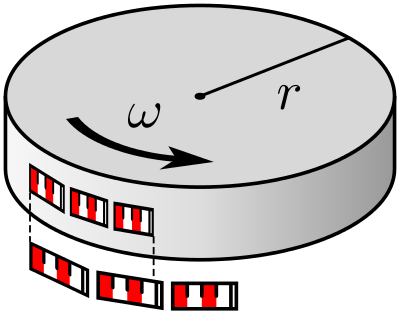
\includegraphics[height=80pt]{assets/Ehrenfest-paradox-disk.png}
    \captionof{figure}{Ehrenfest
    paradox disk}
\end{center}

However, since the radius is perpendicular to the direction of motion,
it will not undergo any contraction. So
\[\frac{\mathrm{circumference}}{\mathrm{diameter}}=\frac{2\pi R \sqrt{1-(\omega R)^2/c^2}}{2R} = \pi \sqrt{1-(\omega R)^2/c^2}.\]
This is paradoxical, since in accordance with Euclidean geometry, it
should be exactly equal to \(\pi\).
\end{quote}

The description above is taken from \emph{Wikipedia: Ehrenfest paradox}\newline (\url{https://en.wikipedia.org/w/index.php?title=Ehrenfest_paradox&oldid=1182372365}).

We can use another metric (张量) to analyze the Ehrenfest paradox. The
metric is
\[\mathrm{d}s^2 = \mathrm{d}r^2 + r^2 \mathrm{d}\theta^2 - c^2 \mathrm{d}t^2.\]

Substitute the relationship between reference frames \(S\) and \(S'\)
\[\left\{
    \begin{array}{l}
        r' = r, \\
        \theta' = \theta - \omega t, \\
        t' = t
    \end{array}
\right.\] in, and we get \begin{align*}
    \mathrm{d}s^2 & = \mathrm{d}r'^2 + r'^2 \left( \mathrm{d}\theta' + \omega \mathrm{d}t \right)^2 - c^2 \mathrm{d}t'^2 \\
    & = \mathrm{d}r'^2 + r'^2 \mathrm{d}\theta'^2 + 2 \omega r'^2 \mathrm{d}\theta' \mathrm{d}t - c^2 \left( 1 - \frac{r'^2 \omega^2}{c^2} \right) \mathrm{d}t'^2.
\end{align*}

Write this in tensor form, and we get
\[\mathrm{d} s^2 = g_{\mu\nu} \mathrm{d}x^{\mu} \mathrm{d}x^{\nu},\]
where \[\mathbf{g} = (g_{\mu\nu}) = \begin{pmatrix}
    1 & 0 & 0 \\
    0 & r'^2 & 2 \omega r'^2 \\
    0 & 0 & - c^2 \left( 1 - \dfrac{r'^2 \omega^2}{c^2} \right)
\end{pmatrix}.\]

\subsection*{(5) Minkowski spacetime
闵可夫斯基时空}\label{minkowski-spacetime-ux95f5ux53efux592bux65afux57faux65f6ux7a7a-2}

In Minkowski spacetime, we express a point within it in this form:
\[\boldsymbol{r} = (ct, x, y, z).\] This is an expression of the world
line (世界线), which is the path that an object traces in 4-dimensional
spacetime.

From \(\boldsymbol{r}\) we can calculate its velocity
\[\boldsymbol{v} = \frac{\mathrm{d} \boldsymbol{r}}{\mathrm{d} \tau} = \frac{\mathrm{d} \boldsymbol{r}}{\mathrm{d}t} \frac{\mathrm{d}t}{\mathrm{d} \tau} = \gamma \frac{\mathrm{d} \boldsymbol{r}}{\mathrm{d}t} = \gamma (c, \dot{x}, \dot{y}, \dot{z}),\]
and thus acceleration \begin{align*}
    \boldsymbol{a} & = \frac{\mathrm{d} \boldsymbol{v}}{\mathrm{d} \tau} = \frac{\mathrm{d} \boldsymbol{v}}{\mathrm{d}t} \frac{\mathrm{d}t}{\mathrm{d} \tau} = \gamma \frac{\mathrm{d} \boldsymbol{v}}{\mathrm{d}t} \\
    & = \gamma \frac{\mathrm{d}}{\mathrm{d}t} \Big[ \gamma \left( c, \dot{x}, \dot{y}, \dot{z} \right) \Big] \\
    & = \gamma \left[ \gamma (0, \ddot{x}, \ddot{y}, \ddot{z}) + \left( c, \dot{x}, \dot{y}, \dot{z} \right) \frac{\mathrm{d} \gamma}{\mathrm{d}t} \right].
\end{align*}

Here, \begin{align*}
    \frac{\mathrm{d} \gamma}{\mathrm{d}t} & = \frac{\mathrm{d}}{\mathrm{d}t} \left( 1 - \frac{\dot{x}^2 + \dot{y}^2 + \dot{z}^2}{c^2} \right)^{- 1/2} \\
    & = - \frac{1}{2} \left( 1 - \frac{\dot{x}^2 + \dot{y}^2 + \dot{z}^2}{c^2} \right)^{- 3/2} \left( - \frac{2 \dot{x} \ddot{x} + 2 \dot{y} \ddot{y} + 2 \dot{z} \ddot{z}}{c^2} \right) \\
    & = \frac{\dot{x} \ddot{x} + \dot{y} \ddot{y} + \dot{z} \ddot{z}}{c^2} \gamma^3.
\end{align*}

Substitute \(\displaystyle \frac{\mathrm{d} \gamma}{\mathrm{d}t}\) into
acceleration, and we acquire \begin{align*}
    \boldsymbol{a} ={} & \gamma^2 (0, \ddot{x}, \ddot{y}, \ddot{z}) + \left( c, \dot{x}, \dot{y}, \dot{z} \right)\frac{\dot{x} \ddot{x} + \dot{y} \ddot{y} + \dot{z} \ddot{z}}{c^2} \gamma^4 \\
    ={} & \biggl(  \frac{\dot{x} \ddot{x} + \dot{y} \ddot{y} + \dot{z} \ddot{z}}{c} \gamma^4, \gamma^2 \ddot{x} + \frac{\dot{x} \ddot{x} + \dot{y} \ddot{y} + \dot{z} \ddot{z}}{c^2} \gamma^4 \dot{x}, \\
    & \gamma^2 \ddot{y} + \frac{\dot{x} \ddot{x} + \dot{y} \ddot{y} + \dot{z} \ddot{z}}{c^2} \gamma^4 \dot{y}, \gamma^2 \ddot{z} + \frac{\dot{x} \ddot{x} + \dot{y} \ddot{y} + \dot{z} \ddot{z}}{c^2} \gamma^4 \dot{z} \biggr).
\end{align*}

From this, we can get 4-dimensional force \begin{align*}
    \boldsymbol{F} = m \boldsymbol{a} = m & \biggl(  \frac{\dot{x} \ddot{x} + \dot{y} \ddot{y} + \dot{z} \ddot{z}}{c} \gamma^4, \gamma^2 \ddot{x} + \frac{\dot{x} \ddot{x} + \dot{y} \ddot{y} + \dot{z} \ddot{z}}{c^2} \gamma^4 \dot{x}, \\
    & \gamma^2 \ddot{y} + \frac{\dot{x} \ddot{x} + \dot{y} \ddot{y} + \dot{z} \ddot{z}}{c^2} \gamma^4 \dot{y}, \gamma^2 \ddot{z} + \frac{\dot{x} \ddot{x} + \dot{y} \ddot{y} + \dot{z} \ddot{z}}{c^2} \gamma^4 \dot{z} \biggr).
\end{align*}

\subsection*{(6) Deduction of relativistic Lagrangian
相对论拉格朗日量的推导}\label{deduction-of-relativistic-lagrangian-ux76f8ux5bf9ux8bbaux62c9ux683cux6717ux65e5ux91cfux7684ux63a8ux5bfc}

Generalized momentum is
\[p = m \frac{\mathrm{d} \boldsymbol{q}}{\mathrm{d} \tau} = \gamma m \dot{q} = \frac{m \dot{q}}{\sqrt{1 - \dot{q}^2 / c^2}}. \quad(1)\]

By definition we know that
\[p \equiv \frac{\partial L}{\partial \dot{q}}.\]

Considering that: (a) \(L = T - V\), (b) \(V(q_1, q_2, \dots, q_s)\)
does not depend on \(\dot{q}_j\) and (c)
\(T(\dot{q}_1, \dot{q}_2, \dots, \dot{q}_s)\) does not depend on
\(q_j\), we can say that
\[p \equiv \frac{\partial \left( L + V \right)}{\partial \dot{q}} = \frac{\partial T}{\partial \dot{q}} = \frac{\mathrm{d} T}{\mathrm{d} \dot{q}}. \quad(2)\]

From \((1)\) and \((2)\), we can acquire an equation for Lagrangian
\(L\):
\[\frac{\mathrm{d} T}{\mathrm{d} \dot{q}} = \frac{m \dot{q}}{\sqrt{1 - \dot{q}^2 / c^2}}.\]

Solve this:
\[\mathrm{d} T = \frac{m \dot{q} \mathrm{d} \dot{q}}{\sqrt{1 - \dot{q}^2 / c^2}} = \frac{m \mathrm{d}\left( \dot{q}^2 \right)}{2 \sqrt{1 - \dot{q}^2 / c^2}} = - \frac{1}{2} mc^2 \mathrm{d} \left( 2 \sqrt{1 - \frac{\dot{q}^2}{c^2}} \right) = - mc^2 \mathrm{d} \sqrt{1 - \frac{\dot{q}^2}{c^2}}.\]

Integrate this, we can get
\[T = - mc^2 \sqrt{1 - \frac{\dot{q}^2}{c^2}}.\]

Thus the Lagrangian
\[L = T - V = - mc^2 \sqrt{1 - \frac{\dot{q}^2}{c^2}} - V.\]

\begin{quote}
作业:推导 \(H = \gamma mc^2 + V\).

答案:\begin{align*}
H & = p \dot{q} - L \\
& = \frac{m \dot{q}}{\sqrt{1 - \dot{q}^2 / c^2}} \dot{q} - \left( - mc^2 \sqrt{1 - \frac{\dot{q}^2}{c^2}} - V \right) \\
& = \frac{m \dot{q}^2}{\sqrt{1 - \dot{q}^2 / c^2}} + \frac{mc^2 \left( 1 - \dfrac{\dot{q}^2}{c^2} \right)}{\sqrt{1 - \dot{q}^2 / c^2}} + V \\
& = \frac{m c^2}{\sqrt{1 - \dot{q}^2 / c^2}} + V \\
& = \gamma mc^2 + V.
\end{align*}
\end{quote}

\chapter{2023/12/25}\label{20231225}

\section{Relationships between events in Minkowski spacetime
闵可夫斯基时空中的事件关系}\label{relationships-between-events-in-minkowski-spacetime-ux95f5ux53efux592bux65afux57faux65f6ux7a7aux4e2dux7684ux4e8bux4ef6ux5173ux7cfb}

Suppose in Minkowski spacetime, we have 2 events, for example,
\((ct_1, x_1, y_1, z_1)\) and \((ct_2, x_2, y_2, z_2)\). Then, the
spacetime interval (时空间隔) between the two events is
\[\Delta s^2 = (c \Delta t)^2 - \Delta x^2 - \Delta y^2 - \Delta z^2 = c^2 \Delta t^2 - \Delta \boldsymbol{r}^2,\]
where \(\Delta \boldsymbol{r}\) is the three-dimensional spatial
distance between the events, the time interval is \(c\Delta t\) and the
three spatial intervals are \(\Delta x\), \(\Delta y\), \(\Delta z\).

In that case, comparing \(\Delta s^2\) with \(0\) seems to be comparing
the distance light travels between the occurrence of the events with
their spatial separation. We now have the following definitions:

\begin{itemize}
\tightlist{}
\item
  If \(\Delta s^2 > 0\), or
  \(c^2 \Delta t^2 > \Delta \boldsymbol{r}^2\), the spatial separation
  is less than the distance light travels and the interval is called
  \textbf{timelike}.
\item
  If \(\Delta s^2 = 0\), or
  \(c^2 \Delta t^2 = \Delta \boldsymbol{r}^2\), the spatial separation
  is equal to the distance light travels and the interval is called
  \textbf{lightlike}.
\item
  If \(\Delta s^2 < 0\), or
  \(c^2 \Delta t^2 < \Delta \boldsymbol{r}^2\), the spatial separation
  is greater than the distance light travels and the interval is called
  \textbf{spacelike}.
\end{itemize}

Fig 29.1 is an illustration of the timelike, spacelike, and lightlike
regions in Minkowski spacetime. In the illustration, the \(z\)-axis is
eliminated for the convenience of drawing.

\begin{center}
    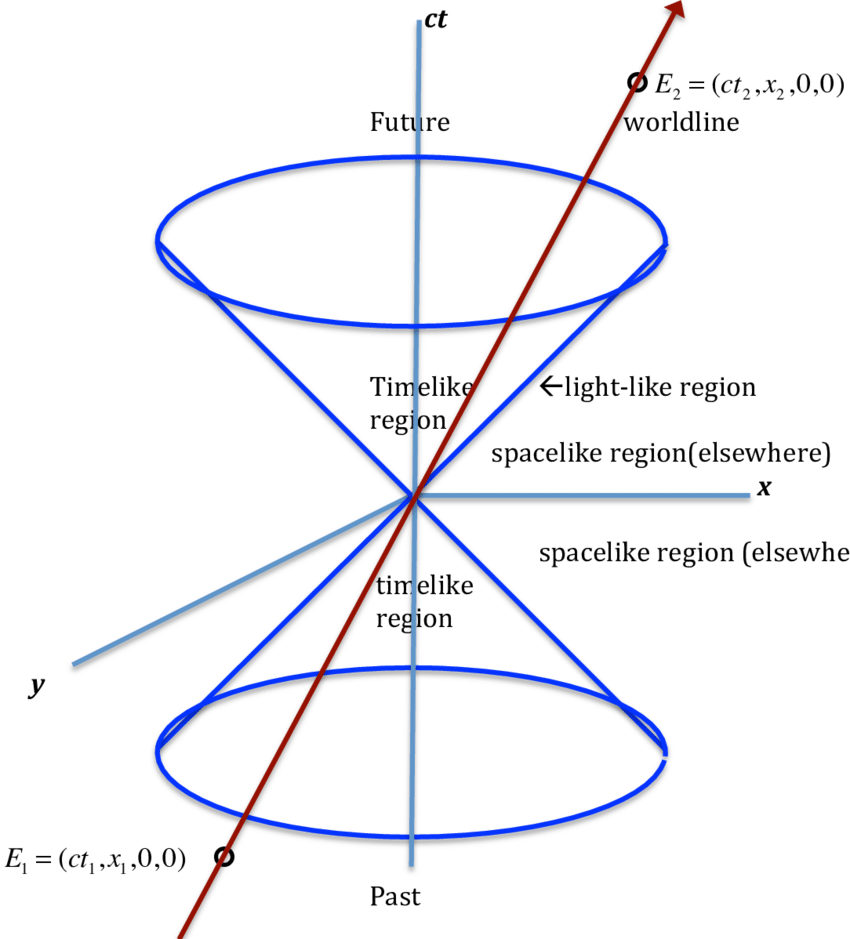
\includegraphics[height=320pt]{assets/Minkowski_spacetime.png}
    \captionof{figure}{Minkowski spacetime and relationships between events}
\end{center}

\emph{相对论的建立中,洛伦兹、庞加莱、闵可夫斯基等人都有杰出贡献,但最终认为爱因斯坦才是相对论的代表性人物,因为只有他形成了相对论中全链条的理论体系。}

\section{Further into relativity
相对论的进一步探讨}\label{further-into-relativity-ux76f8ux5bf9ux8bbaux7684ux8fdbux4e00ux6b65ux63a2ux8ba8}

\subsection*{(1) Postulates in special relativity
狭义相对论的公设}\label{postulates-in-special-relativity-ux72edux4e49ux76f8ux5bf9ux8bbaux7684ux516cux8bbe}

An \textbf{axiom (公理)} or \textbf{postulate (公设)} is a statement
that is taken to be true, to serve as a premise or starting point for
further reasoning and arguments. The difference between these two is
that axioms are statements taken to be true in \textbf{all subjects},
while postulates are statements taken to be true in \textbf{only a
particular subject}.

The two postulates in Einstein's special relativity are:

\begin{enumerate}
\def\labelenumi{\arabic{enumi}.}
\tightlist{}
\item
  The laws of physics have the same form in all inertial reference
  frames.
\item
  Light propagates through empty space with a definite speed \(c\)
  independent of the speed of the observer (or source).
\end{enumerate}

Last time, we talked about length contraction, which states that
\[L = L_0 \sqrt{1 - \frac{v^2}{c^2}}.\]

\begin{quote}
作业:贝尔飞船佯谬是什么?
\end{quote}

Max Born (波恩) put up with the problem of \textbf{Born rigidity}: if
the length of a rigid body would contract at high speeds, why is it a
rigid body?

There is strain (应变) as its definition
\[\varepsilon \overset{\text{def}}{=\!=} \frac{L - L_0}{L_0} = \sqrt{1 - \frac{v^2}{c^2}} - 1 \overset{v \ll c}{=\!=\!=} - \frac{v^2}{2 c^2},\]
and stress (应力) is \[\sigma = \varepsilon E = - E \frac{v^2}{2 c^2},\]
where \(E\) is the Young's modulus of the material.

\emph{从这里可以看出,这里应该是有力的,那么这到底是不是刚体?赵爹说,这是个科学哲学问题,下节课找两个同学辩论一下。}

\subsection*{(2) Time dilation
时间膨胀}\label{time-dilation-ux65f6ux95f4ux81a8ux80c0}

We suppose that there are 2 frames of reference \(S\) and \(S'\), and
\(S'\) is moving at a velocity \(\boldsymbol{v}\) relative to \(S\).

Consider 2 events at the same location in \(S\) happening at
\((t_1, x_1)\) and \((t_2, x_2)\), where \(x_1 = x_2\).

According to the Lorentz transformations, we have
\[t' = \gamma \left( t - \frac{vx}{c^2} \right),\] and with these two
events we get
\[t_2' - t_1' = \gamma \left[ t_2 - t_1 - \frac{v(x_2 - x_1)}{c^2} \right] = \gamma (t_2 - t_1).\]

Here \(\Delta \tau = t_2 - t_1\) is called \textbf{proper time
(固有时)}, and it means the time lapse between the two events in a frame
of reference (stationary frame) in which the two events happen at the
same location. The time measured in a frame of reference which has a
velocity relative to the stationary frame is greater than the proper
time. Thus the duration of the clock cycle of a moving clock is found to
be increased: it is measured to be ``running slow'', and that's where
the name ``time dilation'' comes from.

\section{Symplectic matrices
辛矩阵}\label{symplectic-matrices-ux8f9bux77e9ux9635}

\subsection*{(1) Comparing different formulations of classical
mechanics
对比经典力学的不同表述}\label{comparing-different-formulations-of-classical-mechanics-ux5bf9ux6bd4ux7ecfux5178ux529bux5b66ux7684ux4e0dux540cux8868ux8ff0}

\begin{center}
    \begin{tabular}{|c|c|c|}
        \hline
        \textbf{Formulations} & \textbf{Physical contrast} & \textbf{Mathematical contrast} \\
        \hline
        \rule{0pt}{20pt}
        \textbf{Newtonian mechanics} & $\displaystyle \boldsymbol{F} = \frac{\mathrm{d}p}{\mathrm{d}t}$ & Euclidean geometry \\
        \hline
        \rule{0pt}{20pt}
        \textbf{Lagrangian mechanics} & $\displaystyle \frac{\partial L}{\partial q_j} - \frac{\mathrm{d}}{\mathrm{d}t} \frac{\partial L}{\partial \dot{q}_j} = 0$ & Riemann geometry \\
        \hline
        \rule{0pt}{35pt}
        \textbf{Hamiltonian mechanics} & $\displaystyle \left\{ \begin{aligned} \frac{\partial H}{\partial q_j} &= -\dot{p}_j, \\ \frac{\partial H}{\partial p_j} &= \dot{q}_j \end{aligned} \right.$ & Symplectic geometry \\
        \hline
        \textbf{Equivalency} & Physically equivalent & Mathematically not equivalent \\
        & (物理上等价) & (数学上不等价) \\
        \hline
    \end{tabular}
    \captionof{table}{Comparing different formulations of classical mechanics}
\end{center}

\subsection*{(2) Symplectic matrix
辛矩阵}\label{symplectic-matrix-ux8f9bux77e9ux9635}

Hermann Weyl developed the theory of \textbf{symplectic matrices
(辛矩阵)}, which write the Hamiltonian canonical equations (as shown in
the table above) in matrix form (one-degree): \[\begin{pmatrix}
    \dot{q} \\
    \dot{p}
\end{pmatrix} = \begin{pmatrix}
    0 & 1 \\
    -1 & 0
\end{pmatrix} \begin{pmatrix}
    \displaystyle \frac{\partial H}{\partial q} \\[1.5ex]
    \displaystyle \frac{\partial H}{\partial p}
\end{pmatrix}.\]

If there are \(n\) generalized coordinates, the form of the symplectic
matrix would be \begin{align*}
    \begin{pmatrix}
        \dot{q}_1 \\
        \dot{q}_2 \\
        \vdots \\
        \dot{q}_n \\
        \dot{p}_1 \\
        \dot{p}_2 \\
        \vdots \\
        \dot{p}_n
    \end{pmatrix} & = \begin{pmatrix}
        0 & 0 & \cdots & 0 & 1 & 0 & \cdots & 0 \\
        0 & 0 & \cdots & 0 & 0 & 1 & \cdots & 0 \\
        \vdots & \vdots & \ddots & \vdots & \vdots & \vdots & \ddots & \vdots \\
        0 & 0 & \cdots & 0 & 0 & 0 & \cdots & 1 \\
        -1 & 0 & \cdots & 0 & 0 & 0 & \cdots & 0 \\
        0 & -1 & \cdots & 0 & 0 & 0 & \cdots & 0 \\
        \vdots & \vdots & \ddots & \vdots & \vdots & \vdots & \ddots & \vdots \\
        0 & 0 & \cdots & -1 & 0 & 0 & \cdots & 0 \\
    \end{pmatrix}_{2n \times 2n} \begin{pmatrix}
        \partial H / \partial q_1 \\
        \partial H / \partial q_2 \\
        \vdots \\
        \partial H / \partial q_n \\
        \partial H / \partial p_1 \\
        \partial H / \partial p_2 \\
        \vdots \\
        \partial H / \partial p_n \\
    \end{pmatrix}  \\
    & = \begin{pmatrix}
        \mathbf{0}_n & \mathbf{I}_n \\
        - \mathbf{I}_n & \mathbf{0}_n
    \end{pmatrix} \begin{pmatrix}
        \partial H / \partial q_1 \\
        \partial H / \partial q_2 \\
        \vdots \\
        \partial H / \partial q_n \\
        \partial H / \partial p_1 \\
        \partial H / \partial p_2 \\
        \vdots \\
        \partial H / \partial p_n \\
    \end{pmatrix}.  \\
\end{align*}

Here, $\begin{pmatrix}
        \mathbf{0}_n & \mathbf{I}_n \\
        - \mathbf{I}_n & \mathbf{0}_n
    \end{pmatrix}$ is the symplectic matrix.

\section{Relativistic energy-time relationships
能量-动量关系}\label{relativistic-energy-time-relationships-ux80fdux91cf-ux52a8ux91cfux5173ux7cfb}

\subsection*{(1) Hamiltonian under relativistic conditions
相对论条件下的哈密顿量}\label{hamiltonian-under-relativistic-conditions-ux76f8ux5bf9ux8bbaux6761ux4ef6ux4e0bux7684ux54c8ux5bc6ux987fux91cf}

From last class, we know that
\[L = T - V = - mc^2 \sqrt{1 - \frac{\dot{q}^2}{c^2}} - V.\]

Thus, using Legendre transformation, we get \begin{align*}
    H & = p \dot{q} - L \\
    & = \frac{m \dot{q}}{\sqrt{1 - \dot{q}^2 / c^2}} \dot{q} - \left( - mc^2 \sqrt{1 - \frac{\dot{q}^2}{c^2}} - V \right) \\
    & = \frac{m \dot{q}^2}{\sqrt{1 - \dot{q}^2 / c^2}} + \frac{mc^2 \left( 1 - \dfrac{\dot{q}^2}{c^2} \right)}{\sqrt{1 - \dot{q}^2 / c^2}} + V \\
    & = \frac{m c^2}{\sqrt{1 - \dot{q}^2 / c^2}} + V = \gamma mc^2 + V.
\end{align*}

Let the potential energy \(V\) be \(0\), and we get the form of the
Hamiltonian under relativistic conditions: \[H = \gamma mc^2.\]

\subsection*{(2) Dirac energy-motion relation
狄拉克动量-能量关系}\label{dirac-energy-motion-relation-ux72c4ux62c9ux514bux52a8ux91cf-ux80fdux91cfux5173ux7cfb}

If the mass of a particle when stationary (invariant/proper mass,
固有质量) is \(m_0\), then under relativistic conditions its mass would
become \(m = \gamma m_0\). Thus, the total energy of the particle is
\begin{align*}
    E^2 & = m^2 c^4 = \gamma^2 m_0^2 c^4 = \frac{m_0^2 c^4}{1 - \dfrac{v^2}{c^2}} \\
    & = \frac{\displaystyle m_0^2 c^4 \left( 1 - \frac{v^2}{c^2} + \frac{v^2}{c^2} \right)}{1 - \dfrac{v^2}{c^2}} = m_0^2 c^4 + \frac{m_0^2 c^2 v^2}{1 - \dfrac{v^2}{c^2}} \\
    & = m_0^2 c^4 + \left( \frac{m_0 v}{\sqrt{1 - v^2 / c^2}} \right)^2 c^2 = m_0^2 c^4 + p^2 c^2,
\end{align*} which is the energy-momentum relation.

\subsection*{(3) Klein-Gordon equation
克莱因-戈尔登方程}\label{klein-gordon-equation-ux514bux83b1ux56e0-ux6208ux5c14ux767bux65b9ux7a0b}

We already know the momentum and energy operators in quantum mechanics:
\[\hat{\boldsymbol{p}} = - \mathrm{i} \hbar \nabla \quad \text{and} \quad \hat{E} = \mathrm{i} \hbar \frac{\partial}{\partial t}.\]

Operatorize the energy-momentum relation, and we get
\[E^2 \psi = (m_0^2 c^4 + p^2 c^2) \psi\]
\[\hat{E}^2 \psi = (m_0^2 c^4 + \hat{\boldsymbol{p}} \cdot \hat{\boldsymbol{p}} c^2) \psi\]
\[\left( \mathrm{i} \hbar \frac{\partial}{\partial t} \right)^2 \psi = \left[ \left( {i} \hbar \nabla \cdot {i} \hbar \nabla \right) c^2 + m_0^2 c^4 \right] \psi\]
\[- \hbar^2 \frac{1}{c^2} \frac{\partial^2 \psi}{\partial t^2} = \left( - \hbar^2 \nabla^2 + m_0^2 c^2 \right) \psi\]
\[\left( \frac{1}{c^2} \frac{\partial^2 }{\partial t^2} - \nabla^2 \right) \psi + \left( \frac{m_0c}{\hbar} \right)^2 \psi = 0.\]

Substitute
\(\displaystyle \frac{1}{c^2} \frac{\partial^2 }{\partial t^2} - \nabla^2 = \Box\)
and \(\displaystyle \frac{m_0c}{\hbar} = \mu\) in, and we get
\[\left( \Box + \mu^2 \right) \psi = 0.\]

The Klein-Gordon equation can reflect relativistic effects
(能反映相对论效应), but the second-order derivative with respect to time
contained in it makes it unable to reflect quantum behavior
(反映量子行为).

\emph{薛定谔:这个方程里面有时间的二阶导、没有虚数单位
\({\mathrm{i}}\),我不喜欢,我不发表。}

\emph{克莱因、戈尔登:你嫌弃,我们喜欢啊!于是发表。}

\section[Classical mechanics VS. special
relativity 对比经典力学和狭义相对论]{Comparison between classical mechanics and special
relativity
经典力学和狭义相对论的对比}\label{comparison-between-classical-mechanics-and-special-relativity-ux7ecfux5178ux529bux5b66ux548cux72edux4e49ux76f8ux5bf9ux8bbaux7684ux5bf9ux6bd4}

Below, we compare classical mechanics and special relativity:

\begin{center}
    \begin{tabular}{|c|c|c|}
        \hline
        & Classical mechanics & Special relativity \\
        \hline
        Trait & Stays invariant under & Stays invariant under \\ & Galilean transformations & Lorentz transformations \\
        \hline
        Related Group & Galilean group& Poincaré group \\
        & 伽利略群 & 庞加莱群 \\
        \hline
        Dimension of Group & 10 & 10 \\
        群的维数 & & \\
        \hline
    \end{tabular}
    \captionof{table}{Comparison of Classical Mechanics and Special Relativity}
\end{center}

\paragraph{Poincaré group: 10 dimensions}
\begin{itemize}
\tightlist{}
    \item 4: translation through time or space, one per dimension (时空维度的平移)
    \item 6: Lorentz group:
    \begin{itemize}
\tightlist{}
        \item 3: reflection through a plane, the freedom in orientation of this plane (关于三个平面的反射)
        \item 3: a "boost" in any of the three spatial directions (三个方向的递升)
    \end{itemize}
\end{itemize}

\paragraph{Galilean group: 10 dimensions}
\begin{itemize}
\tightlist{}
    \item 3: translation with uniform velocity (平移变换)
    \item 4: spatial and time translation (时空仿射变换)
    \item 3: rotation (旋转变换)
\end{itemize}

\emph{12月6日的笔记中有更详细的伽利略群的说明。}

\chapter{2023/12/27}\label{20231227}

\section{Dirac equation (1927)
狄拉克方程}\label{dirac-equation-1927-ux72c4ux62c9ux514bux65b9ux7a0b}

\subsection*{(1) The background to proposing the Dirac equation
提出狄拉克方程的背景}\label{the-background-to-proposing-the-dirac-equation-ux63d0ux51faux72c4ux62c9ux514bux65b9ux7a0bux7684ux80ccux666f}

Previously, we have the \textbf{Schrödinger Equation}
\[- { \hbar^2 \over 2m} \nabla^2 \psi + U \psi = \mathrm{i} \hbar {\partial \psi \over \partial t},\]
which can show quantum behavior but not relativistic effects. It
contains the first derivative with respect to time and the second
derivative with respect to space, and thus it does not satisfy Lorentz
invariance.

Later, there was the Klein-Gordon equation
\[\left( \frac{1}{c^2} \frac{\partial^2 }{\partial t^2} - \nabla^2 \right) \psi + \left( \frac{m_0c}{\hbar} \right)^2 \psi = 0,\]
which can show relativistic effects but not quantum behavior.

On this basis, Dirac wanted to put forward an equation containing both
the first derivative with respect to time and space, thus satisfying
both Galilean and Lorentz invariance.

\subsection*{(2) Partial derivation
部分推导}\label{partial-derivation-ux90e8ux5206ux63a8ux5bfc}

We still begin from the momentum and energy operators in quantum
mechanics:
\[\hat{\boldsymbol{p}} = - \mathrm{i} \hbar \nabla \quad \text{and} \quad \hat{E} = \mathrm{i} \hbar \frac{\partial}{\partial t}.\]

Noticing that the deformation (变形) of the energy-momentum relation is
\[E = \sqrt{m_0^2 c^4 + p^2 c^2}, \quad (*)\] and it contains both the
first derivative with respect to time and space, the only thing left to
do for Dirac was to extract the root.

Considering that \(\boldsymbol{p} = (p_x, p_y, p_z)\), we can suppose
the form of the root as
\[\sqrt{a^2 + b^2 + c^2 + d^2} = \alpha_1 a + \alpha_2 b + \alpha_3 c + \beta d.\]
This means that
\[a^2 + b^2 + c^2 + d^2 = \left( \alpha_1 a + \alpha_2 b + \alpha_3 c + \beta d \right)^2,\]
which leads us to \[\left\{
    \begin{array}{l}
        \alpha_i \alpha_j + \alpha_j \alpha_i = 2 \delta_{ij}, \\
        \alpha_i\beta + \beta\alpha_i = 0, \\
        \alpha_i^2 = \beta^2 = 1, \\
    \end{array}
\right.\] where \(i = 1, 2, 3\).

Obviously, for \(\alpha_1, \alpha_2, \alpha_3, \beta\) to have
solutions, these should be matrices. Rewrite these, and we get \[\left\{
    \begin{array}{l}
        \boldsymbol{\alpha}_i \boldsymbol{\alpha}_j + \boldsymbol{\alpha}_j \boldsymbol{\alpha}_i = 2 \delta_{ij} \mathbf{I}, \\
        \boldsymbol{\alpha}_i \boldsymbol{\beta} + \boldsymbol{\beta} \boldsymbol{\alpha}_i = \mathbf{0}, \\
        \boldsymbol{\alpha}_i^2 = \boldsymbol{\beta}^2 = \mathbf{I}. \\
    \end{array}
\right.\]

Here we give the solutions of
\(\boldsymbol{\alpha}_1, \boldsymbol{\alpha}_2, \boldsymbol{\alpha}_3, \boldsymbol{\beta}\)
without proof:
\[\boldsymbol{\beta} = \begin{pmatrix} 1 & 0 & 0 & 0 \\ 0 & 1 & 0 & 0 \\ 0 & 0 & -1 & 0 \\ 0 & 0 & 0 & -1 \end{pmatrix}, \quad \boldsymbol{\alpha}_1 = \begin{pmatrix} 0 & 0 & 0 & 1 \\ 0 & 0 & 1 & 0 \\ 0 & 1 & 0 & 0 \\ 1 & 0 & 0 & 0 \end{pmatrix},\]
\[\boldsymbol{\alpha}_2 = \begin{pmatrix} 0 & 0 & 0 & - \mathrm{i} \\ 0 & 0 & \mathrm{i} & 0 \\ 0 & - \mathrm{i}& 0 & 0 \\ \mathrm{i} & 0 & 0 & 0 \end{pmatrix}, \quad \boldsymbol{\alpha}_3 = \begin{pmatrix} 0 & 0 & 1 & 0 \\ 0 & 0 & 0 & -1 \\ 1 & 0 & 0 & 0 \\ 0 & -1 & 0 & 0 \end{pmatrix}.\]

And the equation \((*)\) becomes
\[\mathrm{i} \hbar \frac{\partial \psi}{\partial t} = \left( - \mathrm{i} \hbar \boldsymbol{\boldsymbol{\alpha}} \cdot \nabla c + \boldsymbol{\beta} mc^2 \right) \psi,\]
where
\(\boldsymbol{\alpha} = (\boldsymbol{\alpha}_1, \boldsymbol{\alpha}_2, \boldsymbol{\alpha}_3)\).
This is the form of Dirac equation. And in natural units, with Feynman
slash notation, we get \[(i\partial \!\!\!/ - m) \psi = 0.\]

This equation can reflect both relativistic and quantum effects, and is
considered one of the most beautiful formulas in theoretical physics.

\section{Hamilton-Jacobi equation
哈密顿-雅克比方程}\label{hamilton-jacobi-equation-ux54c8ux5bc6ux987f-ux96c5ux514bux6bd4ux65b9ux7a0b}

\subsection*{(1) Derivation 推导}\label{derivation-ux63a8ux5bfc-2}

Suppose that we have generalized coordinates \(q_1, q_2, \dots, q_s\).

We already know the Lagrangian \(L(q_j, \dot{q}_j, t)\) and the
Hamiltonian action (哈密顿作用量)
\(S[q(t)] = \int_{t_1}^{t_2} L(q_j, \dot{q}_j, t) \mathrm{d}t\), which
is a functional (泛函) of \(q\).

Maupertuis's principle (莫培督原理) states that the Hamiltonian action
\[S = \int \boldsymbol{p} \cdot \mathrm{d} \boldsymbol{q}.\]

Take the total derivative of \(S\) with respect to time, and we get
\[\frac{\mathrm{d}S}{\mathrm{d}t} = \frac{\partial S}{\partial t} + \sum_{j = 1}^{s} \frac{\partial S}{\partial q_j} \dot{q}_j = \frac{\partial S}{\partial t} + \sum_{j = 1}^{s} p_j \dot{q}_j.\]

Also, because \(\mathrm{d}S = L \mathrm{d}t\) according to the
definition of \(S\), we know that
\[L = \frac{\mathrm{d}S}{\mathrm{d}t} = \frac{\partial S}{\partial t} + \sum_{j = 1}^{s} p_j \dot{q}_j,\]
\[\frac{\partial S}{\partial t} + \sum_{j = 1}^{s} p_j \dot{q}_j - L = 0,\]
\[\frac{\partial S}{\partial t} + H = 0.\]

Also, from above we know that
\(\displaystyle p = \frac{\partial S}{\partial q_j}\), and expressing
the Hamiltonian as
\(\displaystyle H = H \left( q_j, \frac{\partial S}{\partial q_j}, t \right)\),
we get the Hamilton-Jacobi equation:

\[\frac{\partial S}{\partial t} + H \left( q_j, \frac{\partial S}{\partial q_j}, t \right) = 0.\]

\subsection*{(2) Deriving SHO using the Hamilton-Jacobi equation
用哈密顿-雅克比方程推导简谐振子}\label{deriving-sho-using-the-hamilton-jacobi-equation-ux7528ux54c8ux5bc6ux987f-ux96c5ux514bux6bd4ux65b9ux7a0bux63a8ux5bfcux7b80ux8c10ux632fux5b50}

The Hamiltonian of the SHO is
\[H = \frac{p^2}{2m} + \frac{1}{2} kx^2 = \frac{1}{2m} \left( \frac{\partial S}{\partial x} \right)^2 + \frac{1}{2} \omega^2 x^2 = E. \quad (1)\]

From the Hamilton-Jacobi equation, we can get
\[\frac{\partial S}{\partial t} = - H = - E.\]

Adding a function \(W(E, x)\) which does not depend on \(t\), we get
\[S(x, E, t) = - Et + W(E, x). \quad (2)\]

Using \((1)\), we get
\[\frac{\partial S}{\partial x} = \sqrt{2m \left( E - \frac{1}{2}m \omega^2 x^2 \right)};\]
and using \((2)\), we get
\[\frac{\partial S}{\partial x} = \frac{\mathrm{d}W}{\mathrm{d}x},\] and
we get
\[\frac{\mathrm{d}W}{\mathrm{d}x} = \sqrt{2m \left( E - \frac{1}{2}m \omega^2 x^2 \right)},\]
\[\mathrm{d}W = \sqrt{2m \left( E - \frac{1}{2}m \omega^2 x^2 \right)} \mathrm{d}x.\]

Take the partial differential with respect to \(E\), and we get
\begin{align*}
    \frac{\partial W}{\partial E} & = \sqrt{2m} \int \frac{\mathrm{d}x}{2 \sqrt{E - \dfrac{1}{2}m \omega^2 x^2}} \\
    & = \sqrt{\frac{m}{2E}} \int \frac{\mathrm{d}x}{\sqrt{1 - \dfrac{m \omega^2 x^2}{2E}}} \\
    & = \sqrt{\frac{m}{2E}} \sqrt{\frac{2E}{m \omega^2}} \arcsin \left( \sqrt{\frac{m \omega^2}{2E}} x \right) \\
    & = \frac{1}{\omega} \arcsin \left( \sqrt{\frac{m \omega^2}{2E}} x \right).
\end{align*}

According to dimensional analysis, we have
\[\frac{\partial W}{\partial E} - t = \tau,\]
\[\frac{\partial W}{\partial E} = t + \tau = \frac{1}{\omega} \arcsin \left( \sqrt{\frac{m \omega^2}{2E}} x \right),\]
\[x = \sqrt{\frac{2E}{m \omega^2}} \sin \left( \omega t + \varphi_0 \right),\]
where \(\varphi_0 = \omega \tau\).

\section{Poisson bracket
泊松括号}\label{poisson-bracket-ux6ccaux677eux62ecux53f7}

\subsection*{(1) Definition 定义}\label{definition-ux5b9aux4e49-2}

In phase space, we define the Poisson brackets: If we have two functions
\(f(p_j, q_j, t)\) and \(g(p_j, q_j, t)\), then
\[[f, g] = \sum_{j = 1}^{s} \left( \frac{\partial f}{\partial q_j} \frac{\partial g}{\partial p_j} - \frac{\partial f}{\partial p_j} \frac{\partial g}{\partial q_j} \right).\]

Note that many sources also write the Poisson brackets with curly brackets $\{\}$. 

For a random function \(f(p_j, q_j, t)\), we can take the derivative
with respect to time:
\[\frac{\mathrm{d}f}{\mathrm{d}t} = \frac{\partial f}{\partial t} + \sum_{j = 1}^{s} \left( \frac{\partial f}{\partial q_j} \dot{q}_j + \frac{\partial f}{\partial p_j} \dot{p}_j \right).\]

Substitute the Hamiltonian
\(\left\{  \begin{array} {l}  \dfrac{\partial H}{\partial p_j}=\dot q_j \\[1.5ex]  \dfrac{\partial H}{\partial q_j}=-\dot p_j  \end{array} \right.\)
in, and we get
\[\frac{\mathrm{d}f}{\mathrm{d}t} = \frac{\partial f}{\partial t} + \sum_{j = 1}^{s} \left( \frac{\partial f}{\partial q_j} \dfrac{\partial H}{\partial p_j} - \frac{\partial f}{\partial p_j} \dfrac{\partial H}{\partial q_j} \right) = \frac{\partial f}{\partial t} + [f, H].\]

On the occasion that \(f\) does not depend on \(t\), then
\(\dfrac{\partial f}{\partial t} = 0\), and thus
\(\dfrac{\mathrm{d}f}{\mathrm{d}t} = [f, H]\).

\subsection*{(2) Proving Liouville's theorem using
刘维尔定理}\label{proving-liouvilles-theorem-using-ux5218ux7ef4ux5c14ux5b9aux7406}

An equivalent formulation of Liouville's theorem is that
\(\rho(q_j, p_j)\), which is the density of phase points at some point
\((q_j, p_j)\) is conserved, or, in mathematical form,
\[\frac{\mathrm{d} \rho}{\mathrm{d}t} = 0.\]

Take the total derivative of \(\rho\), and we get \begin{align*}
    0 = \frac{\mathrm{d} \rho}{\mathrm{d}t} & = \frac{\partial \rho}{\partial t} + \sum_{j = 1}^{s} \left( \frac{\partial \rho}{\partial q_j} \dot{q}_j + \frac{\partial \rho}{\partial p_j} \dot{p}_j \right) \\
    & = \frac{\partial \rho}{\partial t} + \sum_{j = 1}^{s} \left( \frac{\partial \rho}{\partial q_j} \dfrac{\partial H}{\partial p_j} - \frac{\partial \rho}{\partial p_j} \dfrac{\partial H}{\partial q_j} \right) \\
    & = \frac{\partial \rho}{\partial t} + [\rho, H].
\end{align*}

From this, we know an equivalent formulation of Liouville's theorem:
\[\frac{\partial \rho}{\partial t} + [\rho, H] = 0.\]

\subsection*{(3) Properties 性质}\label{properties-ux6027ux8d28}

There are several properties of the Poisson bracket:

\begin{itemize}
\tightlist{}
\item
  \([f, g] = - [g, f]\);
\item
  \([f, f] = 0\) and \([f, c] = 0\) where \(c = \mathrm{const}\);
\item
  \([f_1 + f_2, g] = [f_1, g] + [f_2, g]\);
\item
  \([f_1 f_2, g] = f_1 [f_2, g] + f_2 [f_1, g]\);
\item
  \(\displaystyle \frac{\partial}{\partial t} [f, g] = [\frac{\partial f}{\partial t}, g] + [f, \frac{\partial g}{\partial t}]\);
\item
  \([q_j, q_j] = [p_j, p_j] = 0\) and \([q_j, p_k] = \delta_{jk}\);
\item
  \([f, [g, h]] + [g, [h, f]] + [h, [f, g]] = 0\).
\end{itemize}

\section{Conclusion and summing up 总结和回顾}\label{conclusion-ux7ed3ux8bba}

\subsection*{(1) ``One''s:}\label{ones}

\begin{itemize}
\tightlist{}
\item
  One center: the beauty of classical mechanics
\item
  One main line: the multiple ways to derive the Simple Harmonic
  Oscillator (SHO)

  \begin{itemize}
\tightlist{}
  \item
    \(\displaystyle \frac{\mathrm{d}E}{\mathrm{d}t} = 0\)
  \item
    the Euler-Lagrange equation
  \item
    the Hamiltonian canonical equations
  \item
    Series expansion
  \item
    Relativistic oscillator (time dilation)
  \item
    Quantum harmonic oscillator
  \item
    Torsional pendulum
  \item
    Physical pendulum
  \end{itemize}
\end{itemize}

\subsection*{(2) ``Two''s:}\label{twos}

\begin{itemize}
\tightlist{}
\item
  Two parts:

  \begin{itemize}
\tightlist{}
  \item
    Newtonian mechanics
  \item
    Analytical mechanics

    \begin{itemize}
\tightlist{}
    \item
      Lagrangian mechanics
    \item
      Hamiltonian mechanics
    \end{itemize}
  \end{itemize}
\end{itemize}

\subsection*{(3) ``Three''s:}\label{threes}

\begin{itemize}
\tightlist{}
\item
  Three geometries:

  \begin{itemize}
\tightlist{}
  \item
    Euclidean geometry
  \item
    Riemann geometry
  \item
    Symplectic geometry
  \end{itemize}
\end{itemize}

\subsection*{(4) ``Four''s:}\label{fours}

\begin{itemize}
\tightlist{}
\item
  Four transformations:

  \begin{itemize}
\tightlist{}
  \item
    Galilean transformation
  \item
    Legendre transformation
  \item
    Lorentz transformation
  \item
    Gauge transformation
  \end{itemize}
\item
  Four basic properties of classical field theory

  \begin{itemize}
\tightlist{}
  \item
    The divergence of the curl of any vector field is equal to zero
  \item
    The curl of the gradient of any scalar field is always the zero
    vector field
  \item
    ``Back Cab''
  \item
    Product operation of Levi-Civita symbols
  \end{itemize}
\item
  Four conserved quantities

  \begin{itemize}
\tightlist{}
  \item
    Energy
  \item
    Momentum
  \item
    Angular momentum
  \item
    Laplace--Runge--Lenz vector
  \end{itemize}
\item
  Four major spaces

  \begin{itemize}
\tightlist{}
  \item
    Euclidean space
  \item
    Configuration space
  \item
    Phase space
  \item
    Minkowski space-time
  \end{itemize}
\item
  Four invariances

  \begin{itemize}
\tightlist{}
  \item
    Galilean invariance
  \item
    Gauge invariance
  \item
    Lorentz invariance
  \item
    Time reversal invariance
  \end{itemize}
\end{itemize}

\subsection*{(5) ``Five''s:}\label{fives}

\begin{itemize}
\tightlist{}
\item
  Five principles

  \begin{itemize}
\tightlist{}
  \item
    The principle of least action
  \item
    Heisenberg's uncertainty principle
  \item
    Virtual work principle
  \item
    D'Alembert's principle
  \item
    Maupertuis's principle
  \end{itemize}
\end{itemize}

\subsection*{(6) ``Six''s:}\label{sixs}

\begin{itemize}
\tightlist{}
\item
  Six major paradoxes

  \begin{itemize}
\tightlist{}
  \item
    Zeno's paradoxes
  \item
    Newton's bucket argument
  \item
    Elevator paradox
  \item
    Twin paradox
  \item
    Bell's spaceship paradox
  \item
    Ehrenfest paradox
  \end{itemize}
\end{itemize}

\subsection*{(7) ``Seven''s:}\label{sevens}

\begin{itemize}
\tightlist{}
\item
  Seven laws

  \begin{itemize}
\tightlist{}
  \item
    Newton's laws of motion (3)
  \item
    Kepler's laws of planetary motion (3)
  \item
    Hooke's law
  \end{itemize}
\end{itemize}

\subsection*{(8) ``Eight''s:}\label{eights}

\begin{itemize}
\tightlist{}
\item
  Eight major groups

  \begin{itemize}
\tightlist{}
  \item
    SO(2)
  \item
    Abel group
  \item
    Lie group
  \item
    Galilean group
  \item
    Poincaré group
  \item
    Lorentz group
  \item
    Space-time translation group
  \item
    Unitary group U(1)
  \end{itemize}
\end{itemize}

\subsection*{(9) ``Nine''s:}\label{nines}

\begin{itemize}
\tightlist{}
\item
  Nine major equations

  \begin{itemize}
\tightlist{}
  \item
    Newton's second law of motion
    \(\displaystyle \boldsymbol{F} = \frac{\mathrm{d}p}{\mathrm{d}t}\)
  \item
    Maxwell's equations
  \item
    Euler--Lagrange equation
  \item
    Hamilton's canonical equation
  \item
    Hamilton--Jacobi equation
  \item
    Navier--Stokes equations
  \item
    Bernoulli's equation
  \item
    Schrödinger equation
  \item
    Klein--Gordon equation
  \end{itemize}
\end{itemize}

\subsection*{(10) ``Ten''s:}\label{tens}

\begin{itemize}
\tightlist{}
\item
  Top ten theorems

  \begin{itemize}
\tightlist{}
  \item
    Noether's theorem
  \item
    Virial theorem
  \item
    Euler's homogeneous function theorem
  \item
    Liouville's theorem
  \item
    Transport theorem in a rotation system
  \item
    Intermediate axis theorem
  \item
    Angular Momentum Theorem
  \item
    König's theorem (柯尼希定理)
  \item
    Gauss's divergence theorem
  \item
    Stokes' theorem
  \end{itemize}
\end{itemize}

\section{Professor Zhao's words
赵爹寄语}\label{professor-zhaos-words-ux8d75ux7239ux5bc4ux8bed}

长江后浪推前浪,世上新人赶旧人。


\appendix % 附录

\newpage
\addcontentsline{toc}{chapter}{Appendix 附录}

\chapter{Philosophy of Science
科学哲学}\label{philosophy-of-science-ux79d1ux5b66ux54f2ux5b66}

\emph{这个部分整理者没什么好说的,只放一下关于这个概念的维基百科页面的机翻或其他相关的文章。}

\section{Self-reference 自指}\label{self-reference-ux81eaux6307}

\emph{Ascending and Descending} by M. C. Escher:

\begin{center}
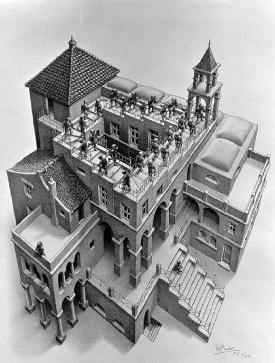
\includegraphics[height=200pt]{../assets/Ascending_and_Descending.jpg}
\captionof{figure}{Ascending and Descending}
\end{center}

Below is the Google translate of \textit{Wikipedia: Self-reference} (\url{https://en.wikipedia.org/w/index.php?title=Self-reference&oldid=1178832976}):

\begin{quote}
自我参照是一个涉及到自己或自己的属性、特征或行为的概念。
它可以发生在语言、逻辑、数学、哲学等领域。

在自然或形式语言中,当句子、想法或公式引用自身时,就会发生自引用。
引用可以直接表达------通过一些中间句子或公式------或者通过一些编码。

在哲学中,自我指涉也指主体能够讲述或指称自身的能力,即具有英语中第一人称单数主格代词``我''所表达的那种思想。

自我参照在数学、哲学、计算机编程、二阶控制论、语言学以及幽默中得到研究和应用。
自我指涉陈述有时是自相矛盾的,也可以被认为是递归的。

\textbf{逻辑、数学和计算}

在古典哲学中,悖论是由自我指涉的概念造成的,例如全能悖论,即询问是否有可能存在一个如此强大的存在,以至于它可以创造出一块它无法举起的石头。
埃皮米尼德悖论``所有克里特岛人都是骗子'',由古希腊克里特岛人说出,是最早有记录的版本之一。
当代哲学有时采用同样的技术来证明一个假定的概念是无意义的或定义不明确的。

在数学和可计算性理论中,自参照(也称为不可预测性)是证明许多系统局限性的关键概念。
哥德尔定理用它来表明,没有任何形式一致的数学系统可以包含所有可能的数学真理,因为它无法证明有关其自身结构的一些真理。
计算理论中的暂停问题等价物表明,总是存在一些计算机无法执行的任务,即推理自身。
这些证明涉及数学悖论的悠久传统,例如罗素悖论和贝里悖论,并最终涉及经典哲学悖论。

在博弈论中,当两个玩家必须模拟彼此的心理状态和行为时,可能会发生未定义的行为,从而导致无限倒退。

在计算机编程中,自引用发生在反射中,程序可以像任何其他数据一样读取或修改自己的指令。
将自引用从潜在的自相矛盾的概念``驯服''为行为良好的递归是计算机科学的伟大成功之一,并且现在经常用于使用``元语言''ML
编写编译器等。 使用编译器来编译自身称为引导。 可以使用汇编程序和 Lisp
等函数式语言来编写自修改代码(对自身进行操作的程序),但在实际编程中通常不鼓励这样做。
计算硬件在触发器中充分利用了自引用,触发器是数字存储器的基本单元,它通过随着时间的推移扩展其术语,将潜在的矛盾逻辑自关系转换为存储器。
以自我引用的方式思考是程序员文化中普遍存在的一部分,许多程序和缩写词都以自我引用的方式命名作为一种幽默形式,例如
GNU(``GNU's not Unix'')和 PINE(``Pine is not Elm'') 。 GNU Hurd
是以一对相互自指的缩写词命名的。

塔珀的自指公式是一种数学好奇心,它绘制了自己公式的图像。

\textbf{生物学}

自我复制的生物学是自我参照的,正如 DNA 和 RNA 复制机制所体现的那样。
康威的生命游戏中发现了自我复制模型,并启发了自我复制 3D 打印机 RepRap
等工程系统。

\textbf{在艺术领域}

当作者在作品本身的背景下引用他或她自己的作品时,文学和电影中就会出现自我指涉。
例如米格尔·德·塞万提斯的《堂吉诃德》、莎士比亚的《仲夏夜之梦》、《暴风雨》和《第十二夜》、丹尼斯·狄德罗的《宿命论者雅克和主人》、伊塔洛·卡尔维诺的《如果在冬夜是一个旅人》、尼古拉·果戈理的许多故事、《迷失在欢乐屋》
约翰·巴特 (John Barth) 的著作、路易吉·皮兰德娄 (Luigi Pirandello)
的《寻找作者的六个人物》(Six Characters in Searching of an
Author)、费德里科·费里尼 (Federico Fellini) 的《8½》和布莱恩·福布斯
(Bryan Forbes) 的《L 形房间》。
推理小说作家塞缪尔·R·德拉尼在他的小说《新星》和《达尔格伦》中利用了这一点。
在前者中,卡廷(一位太空小说家)对一个长期存在的诅咒保持警惕,即小说家在完成任何特定作品之前就去世了。
诺瓦在句子中结束,从而证实了诅咒,并认识到小说家就是故事的作者;
同样,在《达尔格伦》中,德拉尼有一个主角,简称为``基德''(或在某些部分称为``基德''),他的生活和工作是他们自己和小说本身的镜像。
在科幻恶搞电影《太空球》中,导演梅尔·布鲁克斯加入了一个场景,其中邪恶角色正在观看自己故事的录像带副本,其中显示他们无限地``看着自己''。
也许最早的例子是荷马的《伊利亚特》,其中特洛伊的海伦哀叹道:``对于尚未出生的世代/我们将生活在歌曲中''(出现在歌曲本身中)。

艺术中的自我参照与打破第四堵墙和元参照等概念密切相关,后者往往涉及到自我参照。
豪尔赫·路易斯·博尔赫斯的短篇小说在很多方面都运用了自我参照和相关的悖论。
塞缪尔·贝克特的《克拉普的最后一盘磁带》完全由主角聆听并制作自己的录音组成,其中大部分是关于其他录音的。
在 20 世纪 90 年代和 2000
年代,电影自我参照是橡胶现实运动中流行的一部分,特别是在查理·考夫曼的电影《成为约翰·马尔科维奇》和《改编》中,后者在试图描绘自己的创作时,可以说将这一概念推向了突破点。
德罗斯特效应的戏剧化版本。

各种创世神话都援引自我参照来解决创造者的创造物问题。
例如,埃及创世神话中有一位神吞下自己的精液来创造自己。
衔尾蛇是一条神话中的龙,它会吃自己。

《古兰经》包含许多自我参照的例子。

超现实主义画家雷内·马格里特以其自我指涉的作品而闻名。
他的画作《图像的背叛》中包含``这不是烟斗''的字样,其真实性完全取决于``ceci''(英语中的``这个'')一词是指所描绘的烟斗,还是指绘画或文字
或句子本身。 MC 埃舍尔的艺术还包含许多自我指涉的概念,例如手绘本身。

\textbf{用语言}

描述自身的词称为自体词(或自义词)。 这通常适用于形容词,例如
sesquipedalian(即``sesquipedalian''是一个 sesquipedalian
词),但也可以应用于其他词类,例如 TLA,作为``三字母缩写''的三字母缩写。

列出自己的字母和标点符号的句子称为自写字母。

元句子有一种特殊情况,其中元语言中的句子内容与目标语言中的句子内容相同。
这样的一句话本身就是指的。 然而,这种类型的一些元句子可能会导致悖论。
``这是一句话。'' 可以被认为是一个明显正确的自我指涉元句子。
然而,``这句话是假的''是一个元句子,导致了自我指涉悖论。
这样的句子可能会导致问题,例如在法律中,使法律成立的陈述可能相互矛盾或相互矛盾。
库尔特·哥德尔在入籍仪式上声称在美国宪法中发现了这样一个悖论。

当媒体需要报道自己时,偶尔会出现自我引用,例如 BBC 报道 BBC 裁员。
著名的百科全书可能需要包含有关其自身的文章,例如维基百科关于维基百科的文章。

Fumblerules
是一系列良好语法和写作的规则,通过违反这些规则的句子来展示,例如``避免像瘟疫一样的陈词滥调''和``不要使用双重否定''。
该术语是由 William Safire 在已发布的此类规则列表中创造的。

循环定义是一种自我引用,其中术语或概念的定义显式或隐式地包括术语或概念本身。
循环定义被认为是错误的,因为它们仅根据术语本身来定义术语。
这种类型的自我引用可能在论证中有用,但可能导致沟通不够清晰。

副词``特此''以自我指涉的方式使用,例如在``我特此宣布你们为夫妻''这句话中。

\textbf{在流行文化中}

\begin{itemize}
\tightlist{}
\item
  道格拉斯·霍夫施塔特 (Douglas Hofstadter) 的著作,尤其是《Metamagical
  Themas》和《哥德尔》、《埃舍尔》、《巴赫》,运用了许多自我参照的概念,在将这些概念带入
  20 世纪 80 年代的主流知识文化方面具有很大影响力。
  霍夫施塔特定律指出``即使考虑到霍夫施塔特定律,它所花费的时间总是比您预期的要长'',这是自引用格言的一个例子。
  霍夫施塔特还提出了``本书评论''的概念,即一本仅包含其自身评论的书,此后已使用维基和其他技术实现了这一概念。
  霍夫施塔特的``奇怪循环''形而上学试图将意识映射到自我参照上,但在心灵哲学中属于少数派立场。
\item
  ``递归科幻小说''或元小说的子类型现在非常广泛,以至于在新英格兰科幻小说协会的网站上形成了由粉丝维护的参考书目;
  其中一些是关于科幻小说迷的,一些是关于科幻小说及其作者的。
\end{itemize}
\end{quote}

\section{Mathematical structuralism
数学结构主义}\label{mathematical-structuralism-ux6570ux5b66ux7ed3ux6784ux4e3bux4e49}

Emmy Noether (1882\textasciitilde1935)

Mathematical structuralism: 数学结构主义

Mathematical structuralist: 数学结构主义者

Frank Wilczek (2004 Nobel Prize in Physics): ``That theorem (Noether's \newline
theorem) has been a guiding star to 20th and 21st century physics.''

Below is the Google translate of \textit{Wikipedia: Structuralism (philosophy of mathe- \newline matics)} (\url{https://en.wikipedia.org/wiki/Structuralism_(philosophy_of_mathematics)}):

\begin{quote}
\textbf{结构主义(数学哲学)}

结构主义是数学哲学中的一种理论,认为数学理论描述数学对象的结构。数学对象是通过它们在这种结构中的位置来详尽定义的。因此,结构主义认为数学对象不具有任何内在属性,而是由它们在系统中的外部关系定义。例如,结构主义认为,在自然数理论的结构中,数字1被详尽地定义为0的后继者。通过这个例子的推广,任何自然数都是由它在该理论中各自的位置来定义的。数学对象的其他示例可能包括几何中的线和平面,或抽象代数中的元素和运算。

结构主义是一种认识论现实主义观点,它认为数学陈述具有客观的真值。然而,它的中心主张只涉及数学对象是什么类型的实体,而不涉及数学对象或结构具有什么样的存在(换句话说,不涉及它们的本体论)。数学对象的存在类型取决于它们所嵌入的结构的存在类型。结构主义的不同分支在这方面提出了不同的本体论主张。

数学哲学中的结构主义与保罗·贝纳塞拉夫、杰弗里·赫尔曼、迈克尔·雷斯尼克、斯图尔特·夏皮罗和詹姆斯·富兰克林特别相关。

\textbf{历史动机}

结构主义发展的历史动力源于本体论的一个基本问题。自中世纪以来,哲学家们一直在争论数学本体论是否包含抽象对象。在数学哲学中,抽象对象传统上被定义为一个实体:(1)独立于心灵而存在;
(2)独立于经验世界而存在;
(3)具有永恒、不变的特性。传统数学柏拉图主义认为,某些数学元素的集合------自然数、实数、函数、关系、系统------就是这样的抽象对象。相反,数学唯名论否认数学本体论中任何此类抽象对象的存在。

19世纪末20世纪初,一些反柏拉图主义的纲领开始流行。其中包括直觉主义、形式主义和谓语主义。然而,到了
20
世纪中叶,这些反柏拉图主义理论也存在一些自身的问题。这随后导致人们对柏拉图主义的兴趣重新兴起。正是在这种历史背景下,结构主义的动机得以发展。1965
年,Paul Benacerraf
发表了一篇改变范式的文章,题为``数字不可能是什么''。贝纳塞拉夫基于两个主要论点得出结论,集合论柏拉图主义作为数学哲学理论不可能成功。

首先,贝纳塞拉夫认为柏拉图式的方法没有通过本体论检验。他提出了反对集合论柏拉图主义本体论的论证,该论证现在历史上被称为贝纳塞拉夫的认同问题。贝纳塞拉夫指出,存在基本等效的集合论方法将自然数与纯集合联系起来。然而,如果有人要求将自然数与纯集合相关联的``真实''恒等声明,那么当这些基本等价的集合关联在一起时,不同的集合论方法会产生矛盾的恒等声明。这产生了集合论的错误。因此,贝纳塞拉夫推断,这种集合论的错误表明,不可能有任何柏拉图式的方法将数简化为集合来揭示任何抽象对象。

其次,贝纳塞拉夫认为柏拉图式的方法没有通过认识论的检验。贝纳塞拉夫认为,不存在访问抽象对象的经验或理性方法。如果数学对象不是空间或时间的,那么贝纳塞拉夫推断这些对象无法通过知识的因果理论获得。因此,柏拉图主义者提出了一个基本的认识论问题,即提供一个合理的解释,说明具有有限的、经验性思维的数学家如何能够准确地获得独立于思维、独立于世界的永恒真理。正是出于这些考虑,本体论论证和认识论论证,贝纳塞拉夫的反柏拉图批判推动了数学哲学中结构主义的发展。

\textbf{品种}

斯图尔特·夏皮罗将结构主义分为三大思想流派。这些学派被称为前物(ante
rem)、内物(in re)和后物(post rem)。

\textbf{前物结构主义}(``事物之前''),或\textbf{抽象结构主义}或\textbf{抽象主义}(特别与
Michael Resnik、Stewart Shapiro、Edward N. Zalta 和 Øystein Linnebo
相关)有一个
与柏拉图主义相似的本体论(另见模态新逻辑主义)。结构被认为具有真实但抽象和非物质的存在。因此,正如贝纳塞拉夫所指出的,它面临着标准的认识论问题,即解释这种抽象结构与有血有肉的数学家之间的相互作用。

\textbf{内物结构主义}(``在事物中''),或\textbf{模态结构主义}(特别与杰弗里·赫尔曼相关),相当于亚里士多德的实在论(真值的实在论,但关于抽象对象的反实在论
在本体论中)。结构被认为是存在的,因为某些具体系统体现了它们。这会带来常见的问题,即一些完全合法的结构可能会意外地不存在,并且有限的物理世界可能不够``大''以容纳一些其他合法的结构。詹姆斯·富兰克林的亚里士多德实在论也是一种重构主义,认为对称性等结构特性在物理世界中被实例化并且是可感知的。在回答未实例化的结构太大而无法融入物理世界的问题时,富兰克林回答说,其他科学也可以处理未实例化的共性;
例如,颜色科学可以处理任何真实物体上都不会出现的蓝色阴影。

\textbf{后物结构主义}(``事物之后''),或\textbf{取消结构主义}(特别与保罗·贝纳塞拉夫相关),是关于结构的反实在论,其方式与唯名论相似。与唯名论一样,后物方法否认抽象数学对象的存在,其属性除了它们在关系结构中的位置之外。根据这种观点,数学系统是存在的,并且具有共同的结构特征。如果某件事对于一个结构来说是正确的,那么对于所有体现该结构的系统来说也是如此。然而,谈论系统之间``共有''的结构只是有帮助的:它们实际上没有独立存在。
\end{quote}

\section{Square-Cube law
平方-立方定律}\label{square-cube-law-ux5e73ux65b9-ux7acbux65b9ux5b9aux5f8b}

In his twenties, Galileo was asked to calculate hell's exact dimensions, based on Dante's description. Below is the translation of an excerpt from \emph{Galileo, Dante Alighieri, and how to calculate the dimensions of hell} (\url{https://www.abc.net.au/listen/programs/ockhamsrazor/galileo-mapped-dimensions-dante-inferno-hell/7164468}):

\begin{quote}
    \emph{年轻的伽利略·伽利莱被邀请计算地狱的确切尺寸时,他完全搞错了。Len Fisher解释了这个错误——以及伽利略随后的修正——如何奠定了现代科学的基础。}
    
    但丁·阿利吉耶里把地狱想象成地球上一个巨大冰淇淋锥的洞。
    
    地狱的尖端位于地球中心,由地球表面上的拱形屋顶覆盖——就像冰淇淋上的一层巧克力。
    
    伽利略自找麻烦——结果是终身软禁。
    
    屋顶下的空间分为九个层次,最深处为最恶劣的罪犯保留。
    
    14世纪意大利的学术和教会机构字面上解释了但丁对地狱的描绘。
    
    甚至佛罗伦萨学院请来了一个名叫伽利略·伽利莱的年轻博学者,根据但丁的描述计算其精确尺寸。
    
    这对这位24岁的年轻人来说是个绝佳的机会,他开始认真研究。
    
    我们仍然有伽利略宣布结果的两场讲座的记录。它们非常值得一读,比今天许多科学论文更为清晰。
    
    它们也成为了一个明显的警告:对诗意意象的字面解释可能导致最荒谬的结果。
    
    伽利略的第一项任务是计算地狱拱顶有多宽。他知道屋顶的中心位于耶路撒冷,因为但丁在他对炼狱之旅的描述中这样说过:
    
    \begin{quote}
    \emph{太阳已经与地平线相连}
    
    \emph{其子午圈覆盖}
    
    \emph{耶路撒冷的最高点}
    \end{quote}
    
    \begin{center}
        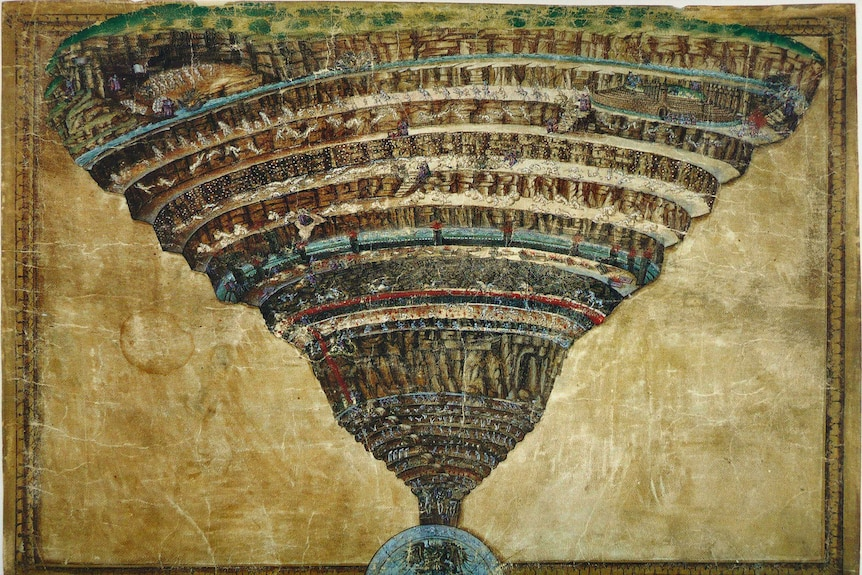
\includegraphics[height=120pt]{assets/Picture_of_Hell.png}
        \captionof{figure}{Hypothesized illustration of Hell}
    \end{center}
    
    但这个子午圈有多宽呢?冰淇淋有多大?
    
    为了证明但丁描述的太阳“与地平线相连”是真实的,伽利略认为诗意意象表明地狱圆顶的直径必须等于地球的半径。
    
    这意味着屋顶的边界将通过法国马赛的西侧和今天的乌兹别克斯坦的塔什干的东侧。
    
    这使得地狱的屋顶成为一个相当大的穹顶——但是,它必须足够大,以容纳现在和将来的居民。
    
    伽利略的下一个问题是计算屋顶的厚度,以防止其坍塌并压垮下面的囚犯。
    
    在这一点上,他又有了一个聪明的想法。伽利略知道佛罗伦萨著名的圣母百花大教堂(今天仍然屹立不倒)宽45米,但只有3米厚。
    
    通过放大比例,他计算出地狱的屋顶必须厚600公里。伽利略最终意识到,这个数字是他计算中的致命错误的产物。但在他注意到之时,他错误的数学描绘地狱的画面已经使他获得了比萨大学的数学讲席。
    
    伽利略没有承认他的错误,也许是为了不失去他的声望和地位,他紧闭双唇,继续思考正确的解决方案。
    
    不过,他在其他事情上可没闷声不响。关于伽利略公开反对教会地球是宇宙中心的观点的故事众所周知,同样众所周知的是这给他惹来了麻烦。
    
    当他在他的《论两大世界系统的对话》中发表他关于日心宇宙的观点时,伽利略犯下了另一个错误。
    
    它采用了对话的形式,其中一个叫Salviati的角色(这就是伽利略自己),一个叫Sagredo的聪明外行(代表现代可能听到RN的人物),以及一个迟钝的回答者叫Simplicio,伽利略关心压制他无思考的观点的人。
    
    伽利略并非完全缺乏政治智慧,他接受了教会当局的指示,将他的日心说称为“假设”,并在他的对话中融入教皇的意见。
    
    他的错误在于把教皇的观点放在Simplicio的口中。伽利略自找麻烦——结果是终身软禁。
    
    在软禁期间,伽利略写了他的另一部著名著作,名为《论两种新科学的对话》。
    
    在这里,他回到了地狱的问题,并最终公开承认了他的第二大错误——地狱穹顶的厚度。
    
    伽利略最初认为屋顶的宽度和厚度可以以相同的方式进行放大——宽度加倍时,他认
    
    为厚度也需要加倍。
    
    那时这是有道理的,但他现在承认自己错了:为了保持结构的强度,厚度必须比宽度更快地增加。
    
    他得出的规则是厚度的立方除以跨度的平方必须保持恒定。
    
    这被称为伽利略的平方立方定律,今天工程师仍在使用。它表明,像梁和屋顶这样的物体在变大时,如果要保持它们的强度,它们必须变得不成比例地更厚。
    
    这甚至适用于动物骨骼,解释了为什么动物的大小存在限制,因为超过一定大小后,它们的骨骼将变得不可能太厚。
    
    它也适用于地狱。当伽利略使用平方立方定律重复他的计算时,他发现屋顶必须如此之厚,以至于几乎没有足够空间容纳所有那些死去的灵魂。
    
    他没有告诉任何人。这可能会让他失去声望和工作。只有在他生命的最后,当他被软禁时,他才把这一切写了下来。
    
    他把地狱及其尺寸的问题转化为现代科学和工程的基础之一。
    
    通过这样做,伽利略确立了一种至今仍然占主导地位的科学方法——坚持将你的信仰与现实相对照。
    
    说到现实:当然,地狱的存在仍然在某些地方存在争议(尽管如果我们使用伽利略的平方立方定律,骨骼能够达到的大小是有限的)。

    \begin{center}
        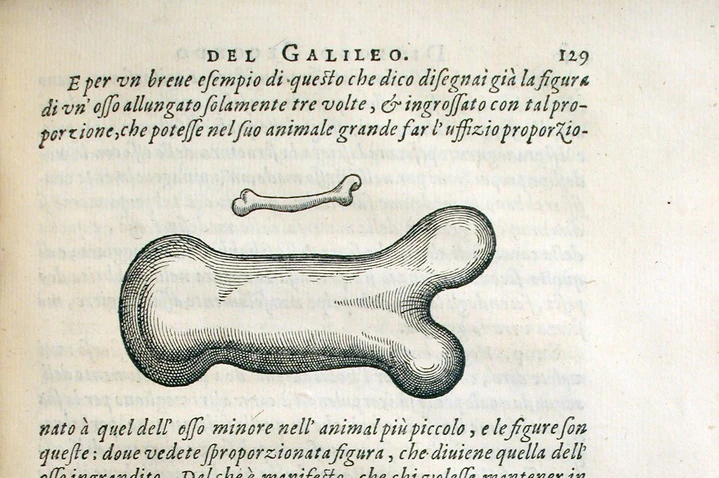
\includegraphics[height=200pt]{assets/The_Bone_in_Square-Cube_law.png}
        \captionof{figure}{The bone in the square-cube law}
    \end{center}
\end{quote}

\newcommand{\wf}{\mathrm{d}}
\newcommand{\e}{\mathrm{e}}
\newcommand{\curl}{\nabla\times}
\newcommand{\divi}{\nabla\cdot}

\chapter{虚位移简介}

\emph{编者注:本节作者为施杰亨。\\\\}

虚位移是分析力学的重要基本概念之一,
一般会在二秋学期的理论力学课程中系统学习,
为使行文不至于太长了(虽然已经很长了),
我们以下仅挑部分简单介绍,完整请参考《理论力学》。
(另外,也可以到赵爹书上看,但不推荐)

\section{约束}

大多数情况下,质点系的运动,除了外力影响外,
还会受内部的一些条件约束。\par
比如,一个单摆,摆锤的位置坐标需要满足\(x^2+y^2=l^2\),这是对位置的几何条件约束;
又如,纯滚条件\(\dot{\varphi} r=\dot{x}\),
这是与速度也有关的约束,称为运动约束,
当然这个条件可以通过积分变成只与位置有关的约束\(R\varphi=x\)。\par
一般的,我们可以把一个由\(n\)个质点组成的力学系统的约束条件表示为
\[f_l(\boldsymbol{r}_1,\boldsymbol{r}_2,
\dots,\boldsymbol{r}_n; \dot{\boldsymbol{r}}_1,
\dot{\boldsymbol{r}}_2,\dots,\dot{\boldsymbol{r}}_n;t)=0,
\quad l=1,2,3,\dots\]
\par
以下我们考虑理想约束,
可以把速度通过积分化为几何约束(可积分的运动约束和几何约束被称为完整约束),
即约束表达式中不含速度
\[f(\boldsymbol{r}_1,\boldsymbol{r}_2,\dots,\boldsymbol{r}_n;t)=0\]
\par
如果约束不直接依赖于时间,
其数学表达式不显含时间,
称为稳定约束;
如果约束明显依赖于时间,
其数学表达式显含时间,
称为不稳定约束。
比如前面提到的单摆即稳定约束。
但是如果我们把摆绳从固定点匀速释放,则约束条件化为
\(x^2+y^2-(l_0+vt)^2=0\),显含时间,是不稳定约束。
\par
当然我们还可以通过广义坐标来表示约束条件。
\[f(q_1,q_2,\dots,q_s;t)=0\]
另外,一个\(n\)自由度的系统,含\(m\)个理想约束,
则独立的广义坐标数为\(s=n-m\)。

\section{变分}

\subsection*{定义}
泛函:设\(C\)是函数(形式)的集合,\(B\)是实数的集合,
如果对\(C\)中每一个函数(形式)都有\(B\)中的实数与之对应,
则称\(F\)是\(q(t)\)的泛函,记为\(F[q(t)]\)。
可以认为泛函是函数的函数,\(q(t)\)是\(F[q(t)]\)的自变量。\par
泛函的变分:如果函数\(q(t)\)是泛函\(F[q(t)]\)定域内一任意函数,
如果\(q(t)\)变化为定域内另一新函数\(\bar{q}(t)\),
则\(\bar{q}(t)\)与\(q(t)\)的差\(\delta q(t)=\bar{q}(t)-q(t)\)是函数\(q(t)\)的变分。

区分以下概念:
\begin{itemize}
    \item 函数的值:取决于自变量的值和函数对应关系(函数形式) \(q(t)\)
    \item 函数的微分:自变量的值的微小改变量引起的函数值的改变量 \(\wf q=\dot{q}\wf t\)
    \item 函数的变分:同一\(t\)时,函数形式的微小改变引起的函数值的变化 \[\delta q(t)=\bar{q}(t)-q(t),\quad\quad\bar{q}(t)=q(t)+\delta q(t)\]
\end{itemize}

\subsection*{举例:}
\subsubsection*{1. \(q(t)=at^2,\,\bar{q}(t)=(a+\delta a)t^2\):}

\[\wf q=2at\wf t\]
\[\delta q=\bar{q}(t)-q(t)=\delta at^2\]

\subsubsection*{2. \(q(t)=t^a,\,\bar{q}(t)=t^{a+\delta a}\):}

\[\wf q=at^{a-1}\wf t\]
\[\delta q=\bar{q}(t)-q(t)=t^a\left(t^{\delta a}-1\right)\]
  
\section{虚位移}

\subsection*{定义}

质点在一个时间间隔\(\wf t\)内\textbf{实际}发生的位移,叫实位移。
用微分符号\(\wf\)表示,即
\[\wf\boldsymbol{r}=\wf x\hat{i}+\wf y\hat{j}+\wf z\hat{k}=\dot{\boldsymbol{r}}\wf t,\]
用广义坐标表示为
\[\wf\boldsymbol{r}=\sum\dfrac{\partial \boldsymbol{r}}{\partial q_i}\wf q_i+\dfrac{\partial \boldsymbol{r}}{\partial t}\wf t.\]

在某时刻\(t\),
在约束条件允许的情况下,
“想象”质点发生了一个极小的位移,就是虚位移,
用一个变分符号\(\delta\)表示。
注意:虚位移不是由时间变化引起的,
只取决于该时刻质点的位置和质点所受的约束条件。即:
\[\delta\boldsymbol{r}=\delta x\hat{i}+\delta y\hat{j}+\delta z\hat{k}, \quad (\delta t=0)\]
用广义坐标表示为
\[\delta\boldsymbol{r}=\sum\dfrac{\partial \boldsymbol{r}}{\partial q_i}\delta q_i.\]

下面考虑约束条件对实位移和虚位移的作用:

\subsubsection*{实位移}

\(\boldsymbol{r}\)和\(\boldsymbol{r}+\wf\boldsymbol{r}\)满足约束条件
\[\begin{cases}
    f(x,y,z,t)=0,\\
    f(x+\wf x,y+\wf y,z+\wf z,t+\wf t)=0
\end{cases}\]
作差
\[\dfrac{\partial f}{\partial x}\wf x+\dfrac{\partial f}{\partial y}\wf y+\dfrac{\partial f}{\partial z}\wf z+\dfrac{\partial f}{\partial t}\wf t=0\]
即
\[\wf f(\boldsymbol{r},t)=\nabla f\cdot\wf\boldsymbol{r}+\dfrac{\partial f}{\partial t}\wf t=0\]

\subsubsection*{虚位移}

\(\boldsymbol{r}\)和\(\boldsymbol{r}+\delta\boldsymbol{r}\)满足约束条件
\[\begin{cases}
    f(x,y,z,t)=0,\\
    f(x+\delta x,y+\delta y,z+\delta z,t)=0,\quad(\delta t=0)
\end{cases}\]
作差得到
\[\dfrac{\partial f}{\partial x}\delta x+\dfrac{\partial f}{\partial y}\delta y+\dfrac{\partial f}{\partial z}\delta z=0\]
即
\[\delta f(\boldsymbol{r},t)=\nabla f\cdot\delta\boldsymbol{r}=0\]
此即约束条件对虚位移的约束。

\subsection*{实位移和虚位移的关系}

实位移是由动力学方程决定的实际发生位移,是唯一确定的。
实位移连接运动轨迹上\(t\)和\(t+\wf t\)对应的两点,\(\wf\boldsymbol{r}\)沿运动轨迹的切向。
\par
虚位移则不需要满足动力学方程,可以有无穷多个。
虚位移连接两个可能的运动轨迹在某一时刻的对应点,
\(\delta \boldsymbol{r}\)使轨迹改变为\(\boldsymbol{r}+\delta\boldsymbol{r}\)。
虚位移需满足几何条件\(\nabla f\cdot\delta\boldsymbol{r}=0\)。
\par
简单地说,二者的区别是:实位移需满足运动方程,虚位移只需满足约束条件。
\par
对稳定约束,实位移是多个虚位移中的一个。
比如前面提到的单摆,
满足约束的虚位移沿圆周切向,有向左或向右两种可能;
而它的实位移还有该时刻的速度方向确定,只能是其中一个方向。
\par
对不稳定约束,实位移与虚位移不一定一致。
比如前面提到的摆绳变长的摆,
虚位移与普通单摆相同,但是实位移还有沿摆绳径向的分量。

\section{虚功原理的应用}

上课例题:如下图,有一根刚性长杆斜靠在墙角,长度为$2l$,与竖直方向的夹角为$\theta$,平衡时水平地面的摩擦力与弹力的比值为$\mu$,竖直墙面光滑。求平衡时的夹角$\theta$的值。

\begin{center}
    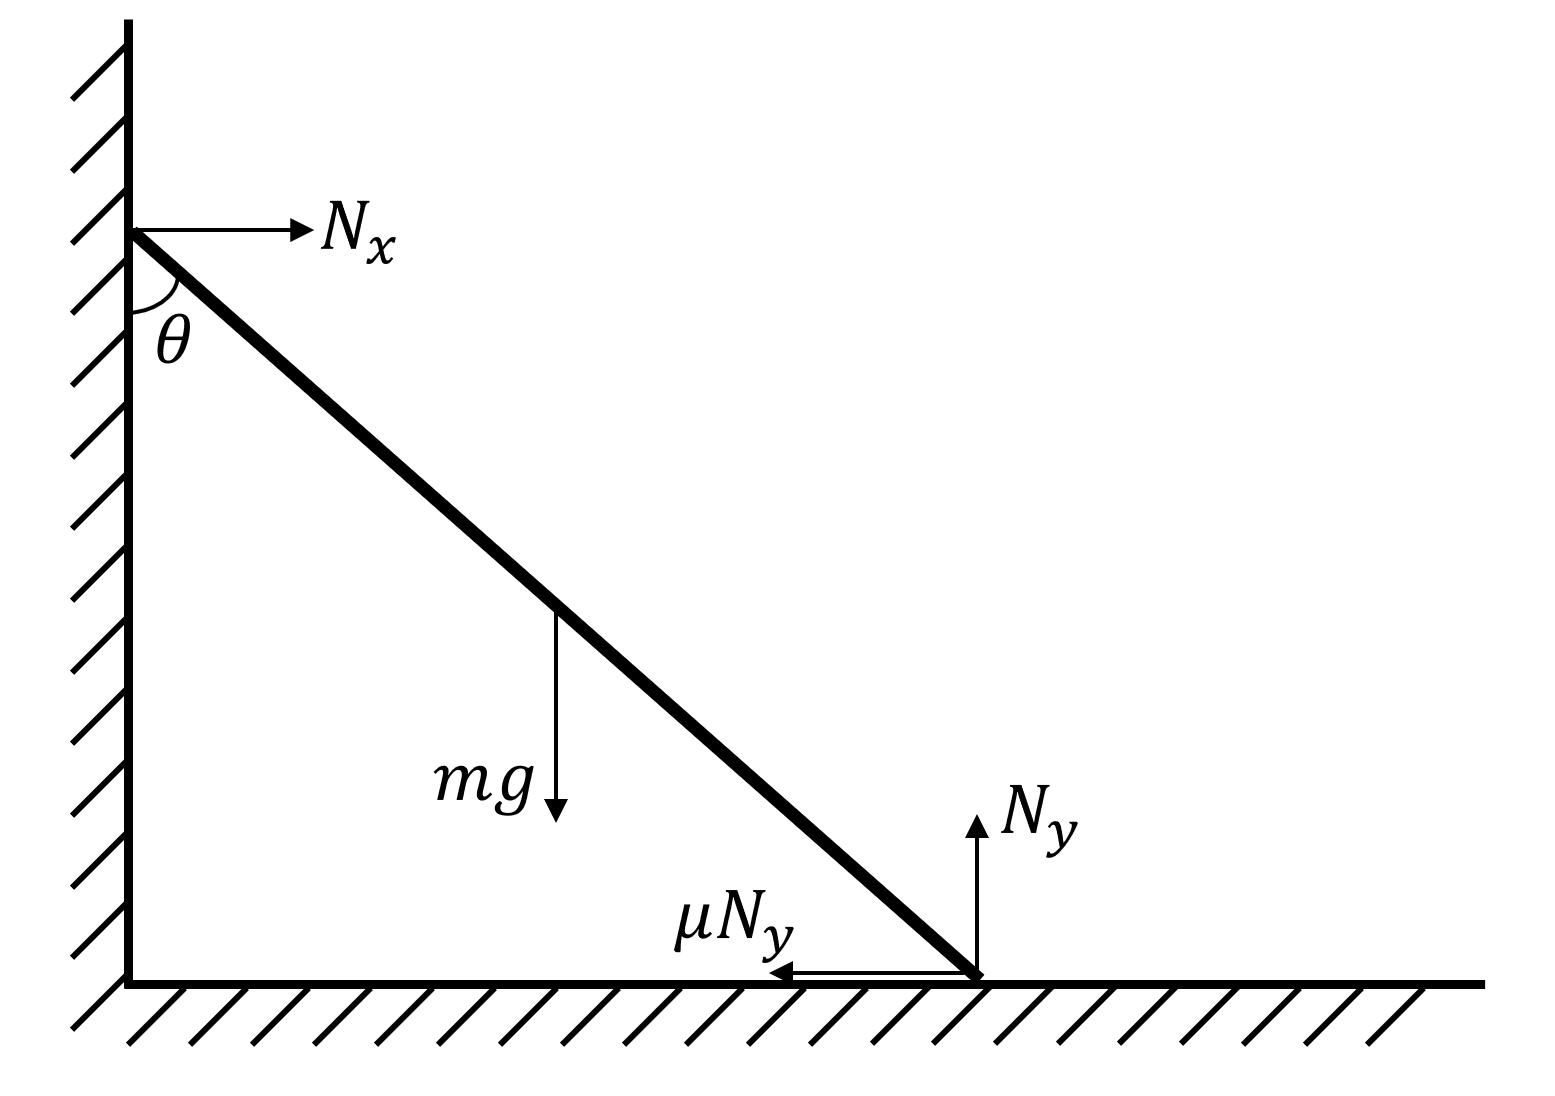
\includegraphics[height=120pt]{assets/Virtual_Displacement_Example.png}
\end{center}

容易发现系统只有一个自由度,
选取广义坐标\(\theta\),则
\[\begin{aligned}
    x_A&=2l\sin\theta,\\
    y_C&=l\cos\theta
\end{aligned}.\]

(此处在使用三角函数时,约束条件已经自动满足,如\(y_A=0,\,x_B=0\)。)

虚位移为
\begin{align*}
    \delta x_A&=2l\cos\theta\delta\theta,\\
    \delta y_C&=-l\sin\theta\delta\theta.
\end{align*}

平衡条件下各主动力总虚功为零
\[\delta W=0,\]
即
\[(-\mu N_Y)\delta x_A-Mg\delta y_C=0.\]

显然\(N_Y=Mg\)
\[(2\mu\cos\theta-\sin\theta)\delta\theta=0.\]
解得
\[\theta=\arctan2\mu.\]

\subsubsection*{}

本题只是虚功原理的简单应用,
我们并不能很好的感受到虚功原理对处理复杂问题的简化。
实际上,虚功原理的主要意义在于简化了约束反力对问题的影响。
我们可以从虚位移满足的条件中看到,约束反力在虚位移上不做功,
即虚功原理只需要处理主动力的做功,这大大简化了运算。


\backmatter % 后记部分

\chapter{后记}

读了这么久的英文,终于又看到中文了。

感谢你能够看到这里。

快乐的时光总是短暂的。在上完赵爹的《力学》课程后,我们还要“重修”《热学》《理论力学》《电动力学》《量子力学》中与本课重合的部分内容。在此,编者认为有义务敬告大家,赵爹的课程覆盖面广是毋庸置疑的,但在仅仅60个课时中试图吃透如此广而多的内容,其内容不深、不精,也是必然的后果。

当初想做这一套笔记只是一个无心之举,并没有想过有朝一日,这套笔记会变成纸质跟大家在现实中见面。感谢大家对编者的厚爱。希望这套笔记,或是能对你的复习起一些帮助,或是在多年后能勾起你对本科的一门课程的回忆。

编者在此祝大家课程满绩,前程似锦!

\begin{flushright}
    陈昱萌

    2024年1月2日于玉泉路
\end{flushright}


\end{document}
